\documentclass[a4paper, 12pt, twoside, openright]{book}
%Options: Sonny, Lenny, Glenn, Conny, Rejne, Bjarne, Bjornstrup
\usepackage[Lenny]{fncychap}

\usepackage[english]{babel}
\usepackage[utf8x]{inputenc}
\usepackage[T1]{fontenc}
\usepackage{amsmath}
\usepackage{amssymb}
\usepackage{slashed}
\usepackage{amsfonts}
\usepackage{fancyhdr}
\usepackage{transparent}
\pagestyle{fancy}
\fancyhf{}
\fancyhead[LE,RO]{\leftmark}
\fancyfoot[C]{\thepage}
\fancyfoot[L]{Gianmarco Tiddia}
\fancyfoot[R]{}
\renewcommand{\headrulewidth}{1pt}
\renewcommand{\footrulewidth}{1.1pt}
\usepackage{hyperref}
\usepackage{subfig}
\usepackage{float}
\usepackage{floatflt}
\usepackage{mathrsfs}
\usepackage{braket}
\usepackage[rightcaption]{sidecap}
\usepackage{wrapfig}
\usepackage[nottoc]{tocbibind}
\usepackage{ucs}
\usepackage{setspace}
\usepackage{afterpage}
\usepackage{graphicx}
\usepackage{emptypage}
\usepackage{wrapfig}
\usepackage{listings}
\usepackage[table,xcdraw,svgnames]{xcolor}
\usepackage{booktabs}% http://ctan.org/pkg/booktabs
\usepackage[nottoc]{tocbibind}
\usepackage{tcolorbox}
\usepackage{charter}
\usepackage{enumitem}
\usepackage[a4paper, top=3.0cm, bottom=3.0cm, headheight=14pt]{geometry}
\geometry{inner=3.5cm,outer=2.5cm}
\newcommand{\HRule}{\rule{\linewidth}{0.8mm}}

\setlength{\headwidth}{\textwidth}

\usepackage{titlesec}
\titleformat{\part}[display]
  {\fontsize{60}{62}\usefont{OT1}{ptm}{m}{n}\selectfont}{Part\ \thepart}{8pt}  
  {\titlerule[0.1pt]\vskip5pt\titlerule[0.5mm]\vskip20pt\Huge\bfseries\filleft}
  %[\vskip20pt\titlerule\vskip5pt\titlerule]


\newcommand{\popI}{\mathcal{P}_1}
\newcommand{\popII}{\mathcal{P}_2}
\newcommand{\popinh}{\mathcal{P}_i}
\newcommand{\NI}{\mathcal{N}_1}
\newcommand{\NII}{\mathcal{N}_2}
\newcommand{\PI}{\text{P}_1}
\newcommand{\PII}{\text{P}_2}
\newcommand{\T}{\mathcal{T}}
\newcommand{\rh}{\nu_\text{h}}
\newcommand{\rl}{\nu_{\ell}}
\newcommand{\rhI}{\nu_\text{h,1}}
\newcommand{\rlI}{\nu_{\ell,1}}
\newcommand{\rhII}{\nu_\text{h,2}}
\newcommand{\rlII}{\nu_{\ell,2}}
\newcommand{\rt}{\nu_\text{t}}
\newcommand{\rtI}{\nu_\text{t,1}}
\newcommand{\rtII}{\nu_\text{t,2}}
\newcommand{\C}{\mathcal{C}}
\newcommand{\Wb}{\mathcal{W}_\text{b}}
\newcommand{\Wc}{\mathcal{W}_\text{c}}
\newcommand{\WIE}{\mathcal{W}_\text{IE}}
\newcommand{\SII}{\mathcal{S}_\text{2}}
\newcommand{\Sb}{\mathcal{S}_\text{b}}
\newcommand{\varSb}{\sigma^{2}_\text{b}}

\newcommand{\ms}{\,\text{ms}}
\newcommand{\MOhm}{\,\text{M}\Omega}
\newcommand{\mV}{\,\text{mV}}
\newcommand{\nS}{\,\text{nS}}
\newcommand{\pA}{\,\text{pA}}
\newcommand{\pF}{\,\text{pF}}
\newcommand{\sps}{\,\text{spikes/s}}

\newcommand{\CM}{C_\text{m}}

\newcommand{\drvd}[1]{\textcolor{gray}{#1}} %% font style for derived parameters
\newcommand{\diff}{\ensuremath{\text{d}}}
\newcommand{\dtsim}{\Delta t}
\newcommand{\Epop}{\mathcal{E}} %% set (hence caligraphic) of excitatory neurons
\newcommand{\Epopsel}{\mathcal{E}_{\text{s}}}
\newcommand{\Epopselfirst}{\mathcal{E}_{\text{s'}}}
\newcommand{\Epopnonsel}{\mathcal{E}_{\text{ns}}}
\newcommand{\exc}{\text{E}}     %% label for ``excitatory'
\newcommand{\ext}{\text{X}}   %% label for ``external''
\newcommand{\inh}{\text{I}}     %% label for ``inhibitory''
\newcommand{\Ipop}{\mathcal{I}} %% set (hence caligraphic) of inhibitory neurons
\newcommand{\leak}{\text{L}}              %% label for ``external''
\newcommand{\RM}{R_\text{m}}
\newcommand{\Stimulus}{\mathcal{S}} %% set (hence caligraphic) of external spike-train generators
\newcommand{\tauM}{\tau_\text{m}}
\newcommand{\tauR}{\tau_\text{ref}}
\newcommand{\tauS}{\tau_\text{s}}
\newcommand{\tauD}{\tau_\text{d}}
\newcommand{\tauF}{\tau_\text{f}}
\newcommand{\note}[1]{\textcolor{red}{[\it #1]}}
\newcommand{\Xpop}{\mathcal{X}} %% set (hence caligraphic) of external spike sources

%\renewcommand{\thefootnote}{\textasteriskcentered}

\def\marg{2pt}
\setlength{\parindent}{2pt}

\begin{document}
\thispagestyle{empty}
\begin{center}
\textbf{\LARGE UNIVERSIT\`A DEGLI STUDI DI CAGLIARI}
\end{center}\par
\rule{\textwidth}{0.1pt}\par
\rule[+0.1\baselineskip]{\textwidth}{0.8mm}
\begin{wrapfigure}{l}{0.01\textwidth} %this figure will be at the right
    
\includegraphics[scale=0.27]{Logo_UNICA.png}
\end{wrapfigure}
\begin{flushright}
\textbf{\Large Faculty of Science}\vspace{5mm}\\
\textbf{\Large Department of Physics}\vspace{5mm}\\
{\Large PhD school of Physics}\vspace{5mm}\\
{\Large Cycle: XXXVI}
\end{flushright}
\begin{flushright}
    \rule{0.5\textwidth}{0.8mm}\par
    \rule[+0.1\baselineskip]{0.5\textwidth}{0.1pt}
\end{flushright}
\vspace{0.8cm}
\begin{center}
{\large THESIS FOR THE DEGREE OF DOCTOR OF PHILOSOPHY}\vspace{0.8 cm}\\
\textbf{\LARGE Large-scale spiking neural networks: from simulation technology to the study of plasticity-driven cognitive processes}
\end{center}
\vspace{0.5cm}
\begin{center}
{\LARGE Gianmarco Tiddia}\vspace{0.5cm}\\
{\Large matr: 200/1053/65055}
\end{center}\par
\rule[+0.1\baselineskip]{\textwidth}{0.1mm}\\
\vspace{-1 cm}
\begin{wrapfigure}{r}{0.61\textwidth} %this figure will be at the right
    {\transparent{0.3}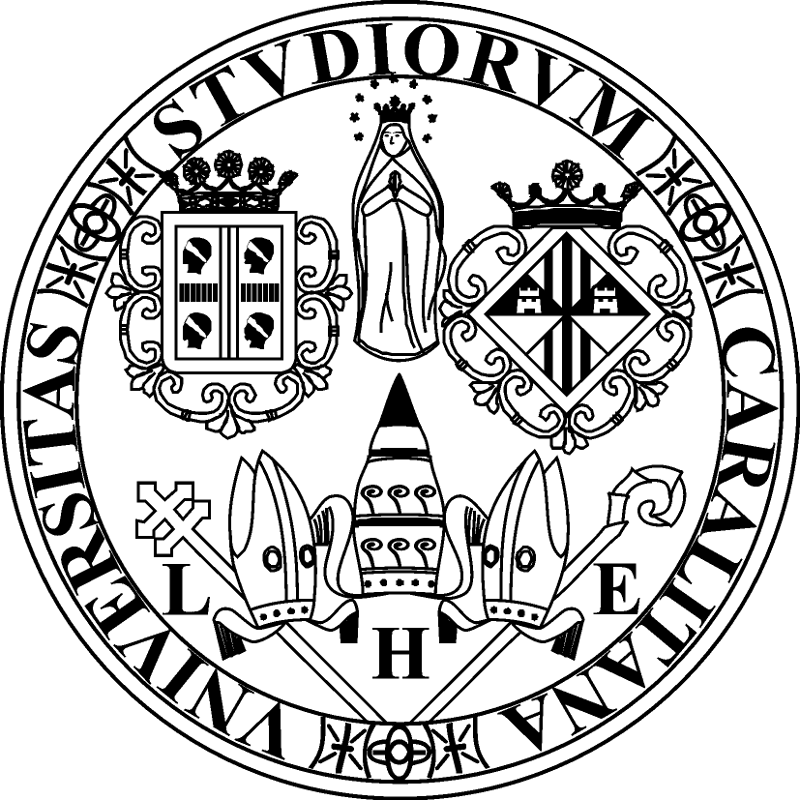
\includegraphics[scale=6.8]{Logo_Unica_BW_transparent.png}}
\end{wrapfigure}
\vspace{1.2 cm}\par
\textbf{\large Academic Advisors}\par\vspace{0.3 cm}
{\large Prof. Bruno Golosio}\par
{\large Dott. Pier Stanislao Paolucci}\par
\vspace{2cm}\par
{\large Submitted 2022/2023}


\fancyfoot[C]{\thepage}
\fancyfoot[L]{Gianmarco Tiddia}
\fancyfoot[R]{}

\mainmatter
\chapter*{Index}
\makeatletter
\@starttoc{toc}
\makeatother
%\listoffigures
\newcommand{\fncyblank }{\fancyhf{}}
%\listoftables
%\renewcommand{\chaptermark}[1]{\markboth{\chaptername \thechapter.\ #1}{\chaptername \thechapter.\ #1}}

%\chapter*{\textbf{Short Abstract}}
%\markboth{ShortAbstract}{ShortAbstract}


\chapter*{List of Publications}
\addcontentsline{toc}{chapter}{List of Publications}
\markboth{ListofPub}{ListofPub}
Publications discussed in this thesis:
\begin{itemize}
    \item \cite{Golosio2021} Golosio B, \textbf{Tiddia G}, De Luca C, Pastorelli E, Simula F and Paolucci PS (2021) Fast Simulations of Highly-Connected Spiking Cortical Models Using GPUs. Front. Comput. Neurosci. 15:627620. doi: \url{https://doi.org/10.3389/fncom.2021.627620}
    \item \cite{Tiddia2022} \textbf{Tiddia G}, Golosio B, Albers J, Senk J, Simula F, Pronold J, Fanti V, Pastorelli E, Paolucci PS and van Albada SJ (2022) Fast Simulation of a Multi-Area Spiking Network Model of Macaque Cortex on an MPI-GPU Cluster. Front. Neuroinform. 16:883333. doi: \url{https://doi.org/10.3389/fninf.2022.883333}
    \item \cite{Tiddia2022_WM} \textbf{Tiddia G}, Golosio B, Fanti V and Paolucci PS (2022) Simulations of working memory spiking networks driven by short-term plasticity. Front. Integr. Neurosci. 16:972055. doi: \url{https://doi.org/10.3389/fnint.2022.972055}
    \item \cite{Golosio2023} Golosio B, Villamar J, \textbf{Tiddia G}, Pastorelli E, Stapmanns J, Fanti V, Paolucci PS, Morrison A and Senk J (2023) Runtime Construction of Large-Scale Spiking Neuronal Network Models on GPU Devices. Appl. Sci. 13(17):9598. doi: \url{https://doi.org/10.3390/app13179598}
    \item \cite{Tiddia2023} \textbf{Tiddia G}, Sergi L and Golosio B (2023) A theoretical framework for learning through structural plasticity.  arXiv:2307.11735 [q-bio.NC]. doi: \url{https://doi.org/10.48550/ARXIV.2307.11735}
\end{itemize}

Additional publications:

\begin{itemize}
    \item \cite{Golosio2021-ThaCo} Golosio B, De Luca C, Capone C, Pastorelli E, Stegel G, \textbf{Tiddia G}, De Bonis G and Paolucci PS (2021) Thalamo-cortical spiking model of incremental learning combining perception, context and NREM-sleep. PLOS Comp. Bio. 17(6): e1009045. doi: \url{https://doi.org/10.1371/journal.pcbi.1009045}
    \item \cite{DeLuca2023} De Luca C, Tonielli L, Pastorelli E, Capone C, Simula F, Lupo C, Bernava I, De Bonis G, \textbf{Tiddia G}, Golosio B and Paolucci PS (2022) NREM and REM: cognitive and energetic gains in thalamo-cortical sleeping and awake spiking model.  	arXiv:2211.06889 [q-bio.NC]. doi: \url{https://doi.org/10.48550/ARXIV.2211.06889} 
\end{itemize}





\chapter*{\textbf{Abstract}}
\addcontentsline{toc}{chapter}{Abstract}
\markboth{ABSTRACT}{Introduction}
The brain is one of the most intricate systems and the quest for simulating the neuronal dynamics has led to the development of several approaches and simulation tools able to represent the behavior of portions of the brain with different levels of detail. Among the different techniques that we can adopt to shed light on neuronal dynamics, mean-field models and spiking neural networks are two of the most relevant, and are introduced in Part \ref{part:intro} of this doctoral thesis. In particular, spiking neural network models have become an effective tool to study brain functions as they capture several aspects of natural neural networks, with every neuron being characterized by a membrane potential and a mechanism to emit electrical pulses for communication with other neurons. While mean-field approaches are suitable for the simulations of models of the entire brain with population resolution, spiking neural networks are able to simulate portions of the brain at cellular level. However, recent computing technologies are paving the way for large-scale simulations through the usage of cutting-edge supercomputer clusters, and it is of fundamental importance for computational neuroscientists to have tools able to take advantage of these technologies. In recent years, Graphical Processing Units (GPUs) established themselves as promising hardware to be employed for such simulations, thanks to their high degree of parallelism, and several GPU-based simulation codes have been developed. In Part \ref{part:I} of this thesis, we describe the GPU code for spiking neural network simulations NEST GPU. Included in the NEST Initiative, it is able to efficiently exploit GPU hardware spanning from consumer GPUs to data-center cards employed in MPI-GPU clusters. The thesis is devoted both to evaluate the performance of such a simulator in the simulation of neuroscientifically relevant models, and, most importantly, to validate the results of the neuronal dynamics with respect to established spiking network simulators such as NEST.


To better understand the link between brain functioning and high-level cognitive processes with low-level neuronal activity, there is the need to provide realistic models both for the neurons and the synapses. Indeed, there is broad consensus in the neuroscientific community that synaptic mechanisms, such as short-term synaptic plasticity and structural synaptic plasticity underlie cognitive processes like working memory and learning. Part \ref{part:II} of this thesis is devoted to the development of simulation and theoretical frameworks able to shed light on the possible relation between these synaptic mechanisms and the previously mentioned cognitive processes. In particular, Chapter \ref{chapter:STP_WM_model} focuses on the simulation of a working memory spiking network driven by short-term plasticity (STP), which is believed to be responsible for the activity-silent mechanisms that characterize working memory networks, while Chapter \ref{chapter:structural_plasticity_theory} presents a theoretical framework able to describe a learning process mediated by structural synaptic plasticity, evaluating the memory capacity of the network as a function of the simulation parameters.


This thesis aims to start facing the challenge of the study of high-level cognitive processes through simulations of large-scale neuronal networks. In a framework in which computing technologies are opening to the realm of large-scale simulations through the usage of GPU clusters, there is a need for simulators capable of exploiting this fast-growing hardware being efficient and, more importantly, reliable. Additionally, modeling neuron and synaptic scale mechanisms can shed light on their impact on high-level cognitive processes such as learning and memory and, together with large-scale simulations at neuron resolution, it would be possible to estimate the relation of these mechanisms and the dynamics of neuronal networks representing a significant portion of the brain. These works are oriented toward the development of more detailed network models, which will pave the way for the usage of these tools in medicine as support for novel therapies.


\part{Introduction}
\label{part:intro}

\fancyfoot[C]{\thepage}
\fancyfoot[L]{Gianmarco Tiddia}
\fancyfoot[R]{Part \thepart}

\chapter{\textbf{Modeling neurons and network dynamics}}
\label{chapter:lif_adex_intro}
%MidnightBlue
\begin{tcolorbox}[colback=white,colframe=DarkRed,title=\textbf{Summary}]
This chapter introduces the topic of neuron modeling and provides the equations of neuronal dynamics used in the thesis to perform spiking network simulations. The chapter, starting from a brief description of the biological neuron and the first neuron modeling approaches, introduces one of the most simple spiking neuron, i.e., the leaky integrate-and-fire neuron model (LIF). Moreover, it will be described the way we can model synapses, distinguishing from current and conductance-based approaches. Finally, firing rate models will be briefly introduced.
\end{tcolorbox}

\section{Biological neurons and how to model them}
In order to model neuron dynamics, we have to be aware of how a neuron works and what mechanisms it exploits to communicate with other neurons.
Neurons are cells which make up the neural tissue, which, together with glial cells, is the main component of the nervous system. They are the elementary units of such a system, and are of large number indeed: a human brain contains around $86\times 10^{9}$ neurons \cite{Azevedo2009}. Each neuron is provided with thousands of synapses to communicate with other neurons\footnote{It is estimated that neurons of the cerebral cortex have, on average $10^{4}$--$10^5$ synapses each \cite{Cragg1975, Alonso-Nanclares2008}.}, forming intricate networks. Neurons communicate using a combination of electrical and chemical signals which are delivered to all the neurons they are connected with. This peculiar communication method requires a likewise peculiar cell structure. Indeed, neurons are composed of three basic structures such as the \textit{soma}, which is the cell body, and extensions such as the \textit{axon} and the \textit{dendrites}, which have the role of transmitting or receiving signals, respectively. Axon and dendrites are not simple extensions of the body cell, since some cellular components are only located in the latter, and also the cellular membrane itself has different characteristics.\\
The effect of the electric pulses exchanged between neurons result in a change of the neuronal membrane electric potential.
Indeed, a resting neuron shows a membrane electric potential because of a difference of concentration of certain ions between the inside and the outside of the membrane, which leads to a difference in the membrane electric potential according to the Goldman equation. The main ions involved in this process are sodium ($Na^+$) and potassium ($K^+$), with a resting membrane potential of around $-70$\,mV. A neuron emits a short and intense signal called \textit{action potential} (or \textit{spike}) when the membrane is sufficiently depolarized. Indeed, a depolarization of the membrane opens voltage-gated channels leading to a flux of sodium ions towards the outside of the neuron. A sufficiently depolarized membrane (around $-55$\,mV) leads to a positive feedback mechanism and to the emission of an action potential that propagates towards the axon to be transmitted to other neurons. After that, the membrane potential is restored to the resting value through specific ion pumps.\\
In order to provide detailed neuron models able to explain the dynamics of a neuron membrane potential we can adopt a relatively simple yet powerful approach, based on the construction of a so-called \textit{equivalent circuit}, which has the aim of capturing the main aspects of the mechanisms briefly discussed above that describe the neuronal dynamics. Next, it will be shown one of the most famous neuron models, based on the design of an equivalent circuit, i.e., the Hodgkin-Huxley model. This model has not been employed for the aims of this thesis, but it is of fundamental importance since it represents the first neuron model with a high predictive power.

\subsection{Modeling using equivalent circuits}
The idea of describing the neuronal membrane and its dynamics using equivalent circuits comes from a phenomenological approximation for the description of membrane and ion channels. First of all, the membrane in such a models is described as a capacitor, since its impermeability prevents ions from passing through it and the charge is represented by the ion concentrations in proximity of the inside and outside of the membrane. The only elements that enable an ion flux through the membrane are the ion channels, which can be modeled using variable resistors and voltage generators to describe the ion flux based on the membrane potential.\\
The following is a typical example of neuron model described by an equivalent circuit. Developed in 1952, the Hodgkin-Huxley (HH) model \cite{Hodgkin1952} is a semi-empirical model which takes into account the dynamics of sodium and potassium ions, together with a non-voltage dependent leakage channel, which takes into account minor contributions driven from the rest of ion species.
Figure \ref{fig:HH_circuit_scheme} shows the circuit scheme of the model. Supposing that an input current $I$ arrives from the outside of the membrane, we can use the conservation of charge to derive an differential equation on the membrane potential $V_{\text{m}}$. The equation will have the form $C_{\text{m}}\dot{V_{\text{m}}}=I-I_{\text{K}}-I_{\text{Na}}-I_{\text{L}}$, and the ion currents can be modeled using channel conductance.

\begin{figure}[H]
    \centering
    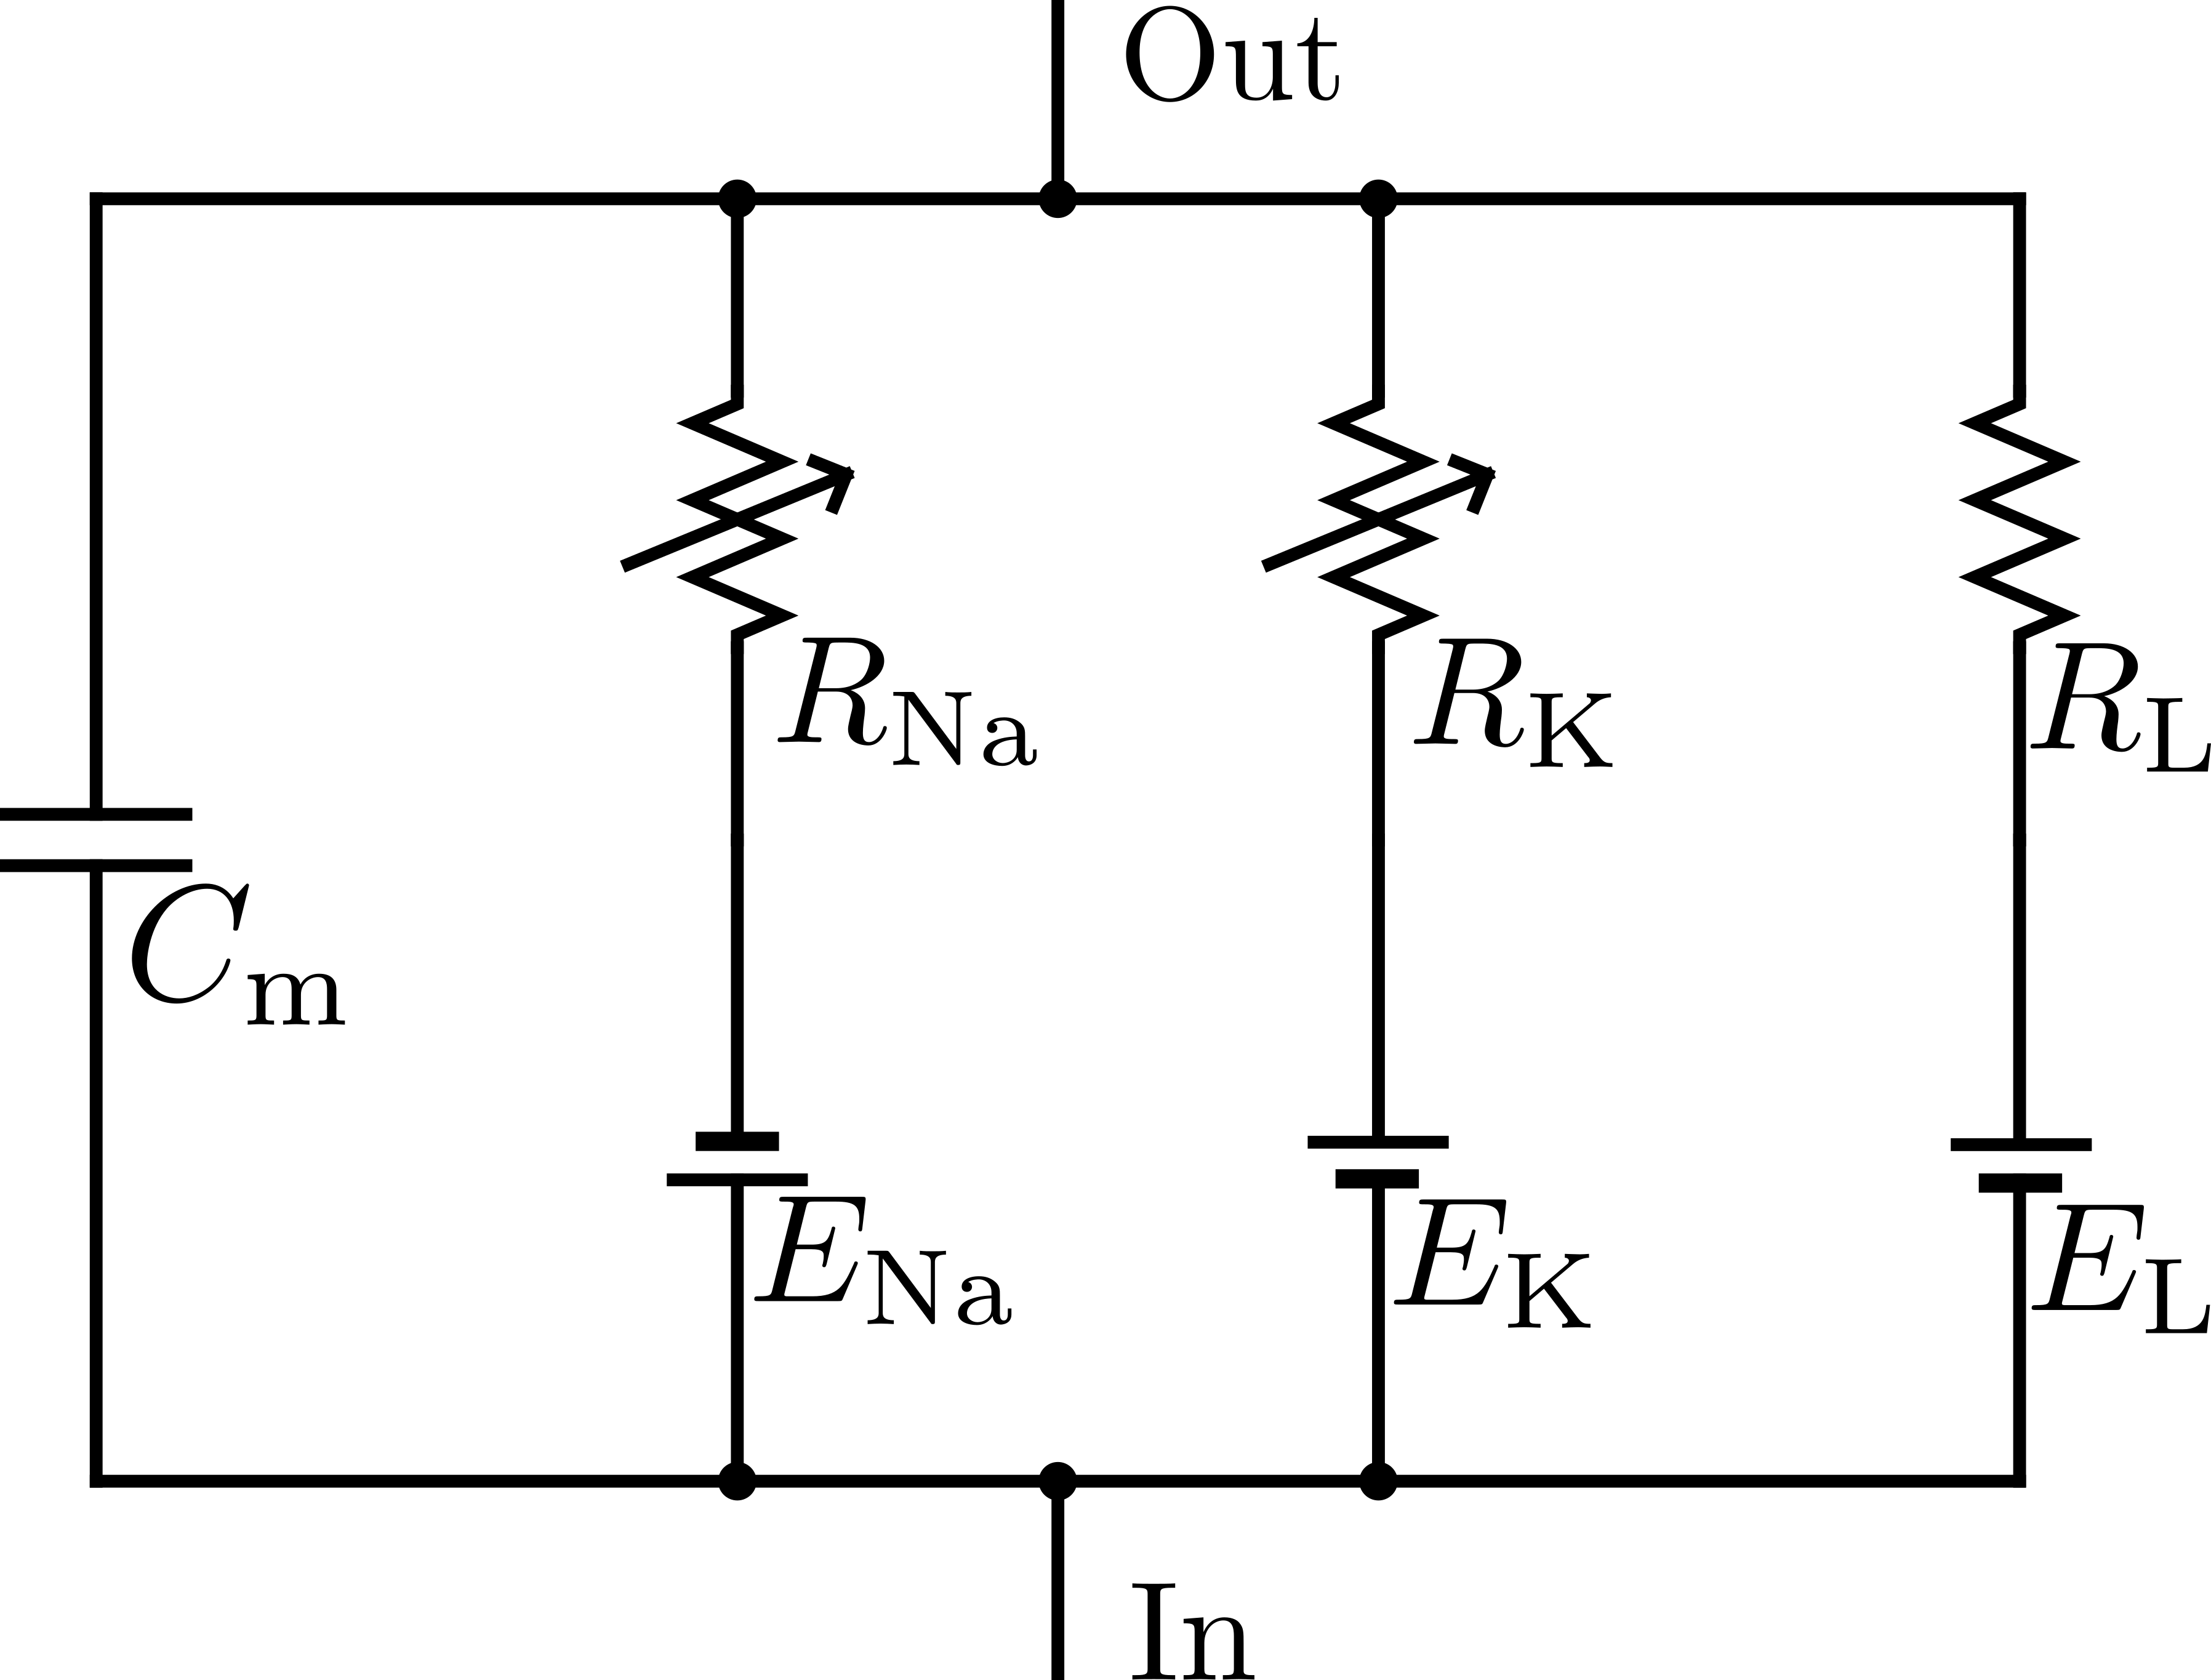
\includegraphics[width=0.5\columnwidth]{figures/HH_circuit.png}
    \caption{Equivalent circuit for the Hodgkin-Huxley model. Out and In represent, respectively, the outside and the inside of the neuron. Generator and resistive element represent sodium (Na), potassium (K) and leakage (L) channels.}
    \label{fig:HH_circuit_scheme}
\end{figure}

The complete set of equations describing the HH model is
\begin{equation}
    \begin{split}
        C_{\text{m}}\dot{V_{\text{m}}} &= I - g_{\text{K}}(V_{\text{m}}-E_{\text{K}}) - g_{\text{Na}}(V_{\text{Na}}-E_{\text{Na}}) - g_{\text{L}}(V_{\text{m}} - E_{\text{L}})\\
        &= I - g_{\text{K}\infty}n^4(V_{\text{m}}-E_{\text{K}}) - g_{\text{Na}\infty}m^3h(V_{\text{Na}}-E_{\text{Na}}) - g_{\text{L}}(V_{\text{m}} - E_{\text{L}})\\
        \dot{n} =& \alpha_{n}(V_{\text{m}}) (1-n) - \beta_{n}(V_{\text{m}})n\\
        \dot{m} =& \alpha_{m}(V_{\text{m}}) (1-m) - \beta_{m}(V_{\text{m}})m\\
        \dot{h} =& \alpha_{h}(V_{\text{m}}) (1-h) - \beta_{h}(V_{\text{m}})h
    \end{split}
\end{equation}
where the $\alpha$ and $\beta$ functions represent the nonlinear voltage dependence and are obtained through experimental observations. The interesting part is the fact that, using the variables $n,m,h$ we are able to provide the description of sodium and potassium channel dynamics: $n$ and $m$ are defined as \textit{potassium activation gate} and \textit{sodium activation gate} since their value changes as a function of the membrane potential. The variable $h$ is called \textit{sodium inactivation gate} and regulates the dynamics of the channel as soon as the action potential is emitted. This variable leads to a short time period, called \textit{refractory period}, during which the neuron is not able to depolarize the membrane.\\
Such a model is able to describe in detail the dynamics of the membrane potential of a neuron and the mechanism of spike emission by modeling the dynamics of the most relevant ion channels. However, we can guess that simulating a large-scale networks of HH neurons can be arduous, since to compute the dynamics of each neuron a system of four differential equations has to be solved numerically. Thus, there would be the need for simpler neuron models in order to pave the way for large-scale simulation within a reasonable computing time, still capturing the main aspects of the dynamics of a neural network. These neuron models are described in the next section.

\section{Integrate-and-fire neuron models}
Although the Hodgkin-Huxley model provides a detailed description of the dynamics of a neuron membrane potential, and several models taking account of diverse ionic current have been developed during the last decade, the non linearity of their differential equations can result in computationally expensive simulations when a large number of neurons is employed. For this reason, large-scale spiking neural network simulations rarely employ this model. Indeed, the need for building large-scale networks of neurons within a reasonable time-to-solution time requires a compromise on the single neuron modeling. In this regard, \textit{integrate-and-fire} models were introduced to provide a simplified yet computationally efficient description for the dynamics of single neurons. Starting from the work of Lapicque in 1907 \cite{Brunel2007_lapique} and developed around the 1960s (see \cite{Brunel2007} for a nice report), integrate-and-fire models describe the relationship between current inputs received by the neuron and its membrane potential using differential equations (or systems of differential equations), with membrane potential changed that can be modeled in different ways depending of a \textit{voltage threshold}, a parameter that is not present in models such as the HH. When the membrane potential is below the threshold, if the neuron is not injected by a current, the membrane behaves passively acting like a discharging capacitor tending towards a resting membrane potential value. When the threshold is reached (ergo when the neuron has received enough current input), the model \textit{fires} a spike and suddenly after resets the membrane potential to a baseline level. Thus, there is no modeling of the ion channel dynamics that lead to the emission of the action potential, neither to the dynamics that takes place after the emission during which ion concentration are restored before the neuron is able to fire again. The latter is simply modeled defining a \textit{refractory time}, during which the model does not integrates any input.\\
Thus, integrate-and-fire models are able to provide us only the time at which the spike is fired. Indeed, these models assume that, since the shape of the action potential is approximately the same among all the spikes fired by neurons, the information to be transmitted to other neurons is not contained in the shape itself, rather by the time at which spikes are emitted. Ergo, the description of the action potential can be discarded and only the spike time can be considered as a relevant quantity able to make neurons communicate with each other.

Next sections describe some of the most used integrate-and-fire models, such as the leaky integrate-and-fire and the adaptive exponential integrate-and-fire neuron models, mainly following the text Neuronal Dynamics \cite{Gerstner2014}.

\subsection{Leaky integrate-and-fire (LIF)}
\label{sec:lif_description}
The leaky integrate-and-fire model (LIF) is the most simple model of this kind of neurons and is described by the most simple equivalent circuit for the neuronal membrane, i.e., an RC circuit. The circuit is also provided with a voltage source to have a defined resting membrane potential. Following figure provides a scheme of the model.

\begin{figure}[H]
    \centering
    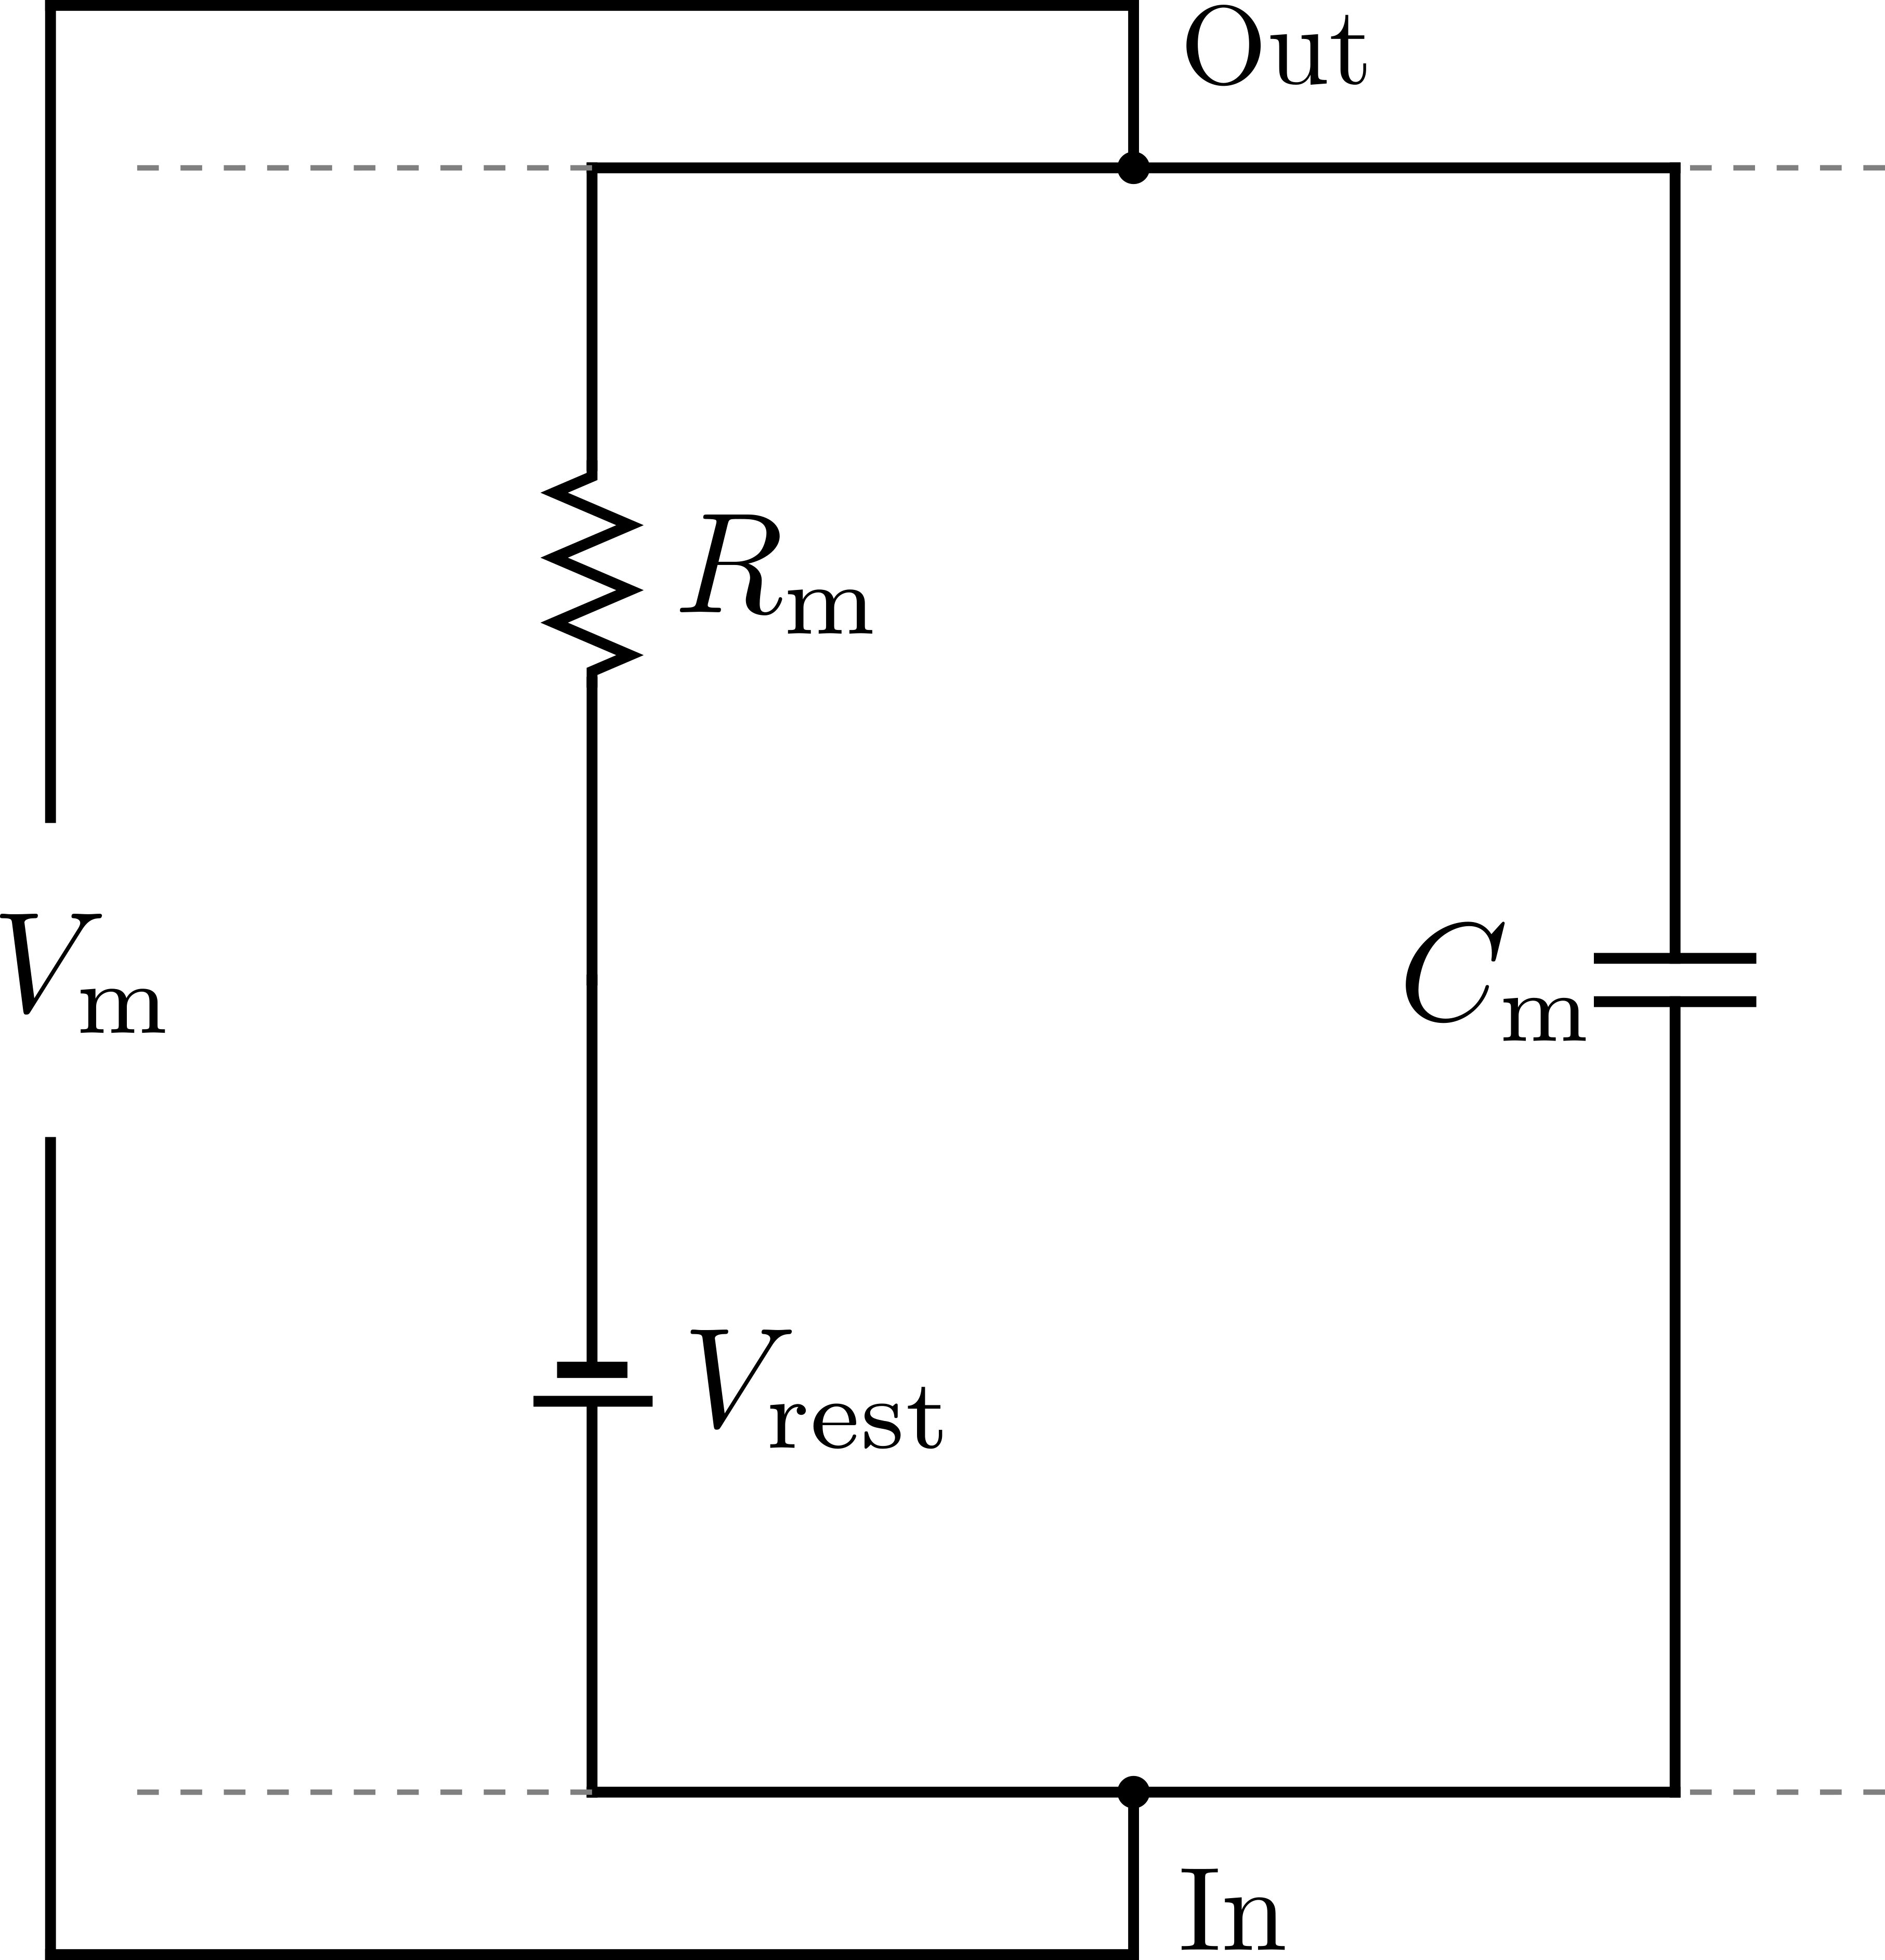
\includegraphics[width=0.3\columnwidth]{figures/LIF_RC_circuit.png}
    \caption{Leaky integrate-and-fire neuron model equivalent circuit. The circuit comprises a capacity ($C_{\text{m}}$), a resistance ($R_{\text{m}}$) and a generator with voltage $V_{\text{rest}}$.
    The membrane potential $V_{\text{m}}$ measured between the inside and the outside of the membrane. The gray lines indicate that this circuit represents a portion of the whole neuronal membrane.}
    \label{fig:RC_circuit_LIF}
\end{figure}

To derive the equations describing the dynamic of the LIF neuron model we have to consider an input current $I(t)$ which, using the law of current conservation, can be split as follows:
\begin{equation}
    I(t) = I_{R_{\text{m}}} + I_{C_{\text{m}}} = \dfrac{V_{\text{m}} - V_{\text{rest}}}{R_{\text{m}}} + C_{\text{m}}\dot{V}_{\text{m}}
    \label{eq:lif_RC}
\end{equation}
where $\dot{V}_{\text{m}}$ is the derivative of the membrane potential with respect to the time $t$. Calling $\tau_{\text{m}}= R_{\text{m}} C_{\text{m}}$ and $\Delta V = V_{\text{m}} - V_{\text{rest}}$ we have that
\begin{equation}
    \tau_{\text{m}}\dot{V}_{\text{m}} = - \Delta V + R_{\text{m}} I(t)
\end{equation}
From the equation above we derive the description of the behavior of the membrane below the voltage threshold $V_{\text{th}}$
\begin{equation}
    V_{\text{m}}(t) = V_{\text{rest}} + \Delta V \exp{\Bigl( \frac{t-t_0}{\tau_{\text{m}}} \Bigr)}
    \label{eq:lif_subthreshold}
\end{equation}
when $t>t_0$ and using the initial condition $V_{\text{m}}(t_0) = V_{\text{rest}} + \Delta V$. Thus, according to Equation \eqref{eq:lif_subthreshold}, if no additional input is provided after $t_0$, the membrane potential of the neuron decays exponentially with a time constant $\tau_{\text{m}}$ reaching the resting value $V_{\text{rest}}$.\\
If the input signal received by the neuron is sufficient for it to reach the potential threshold $V_{\text{th}}$, ad discussed before, 
the membrane potential drops to a reset value $V_{\text{reset}}$ suddenly after the time of spike emission $t_{f}$
\begin{equation}
    \lim_{\epsilon \rightarrow 0^+} V(t_{f} + \epsilon) = V_{\text{reset}}
\end{equation}
and remains clamped at this value after the spike emission for a time $t_{\text{ref}}$, which is the refractory time.\\
This model has been employed in large-scale models such as the cortical microcircuit of \cite{Potjans2012}, in particular for its simplicity and the fact that it can be integrated using efficient integration methods such as \cite{Rotter1999}. Moreover, it is possible to obtain closed form expressions to derive, for instance, the external current needed to elicit a defined change in the membrane potential. We see some additional calculations on this model later in this chapter, to support the description of the spiking network models presented in this thesis.\\
However, such an elementary model has some limits. For example the linearity of the model makes the response of an input independent from the value of the membrane potential, and in case of spike emission, after the neuron membrane potential is reset, all the information related to the previous activity is lost.
Indeed, it has been shown that neurons have some mechanisms related to the possibility of keeping a "memory" of their previous synaptic activity, since repetitive stimulus leads to a lower response over time. This mechanism is called \textit{adaptation}, and can be added into integrate-and-fire neuron models with non linearity. Thus, instead of having a neuron model described by a linear differential equations we can have something like
\begin{equation}
    \tau_{\text{m}}\dot{V}_{\text{m}} = f(V_{\text{m}}) + R_{\text{m}} I(t)
\end{equation}
with $f(V_{\text{m}})$ being a non-linear term. An example of a integrate-and-fire model able to describe this mechanism is called Adaptive exponential integrate-and-fire (AdEx) \cite{Brette2005}. Such a model is able, after appropriate parameter tuning, to show a voltage trace compatible with the HH model when the same input current is given, meaning that an integrate-and-fire model, despite the simplicity related to the threshold mechanism and the need of a compromise between computational cost and realistic behavior, can be able to reproduce analogous results of a more detailed semi-empirical model.\\
For the purpose of this thesis we employ leaky integrate-and-fire neurons, in particular because of the possibility of finding close form solutions for a proper choice of the inputs to be given to the neurons. In this regard, some examples will be shown later in this chapter.
The next section shows how to model synaptic response, i.e. how we can model the shape of the postsynaptic potential (PSP) when a neuron receives a spike.

\section{Modeling synaptic response}
Here we present a brief introduction on synaptic response, functional to the neuron models employed in this work. For an exhaustive discussion please refer to Modeling Synapses \cite{modeling_synapses}, a chapter of \cite{DeSchutter2009}, from which the following discussion is drawn.\\
As we already discuss in the first section, the presynaptic spike depolarizes the synaptic terminal, causing the influx of Calcium ions that trigger the neurotransmitter release. Then, neurotransmitters bound to receptors in the postsynaptic terminal, leading to a ionic current across the postsynaptic neurons and polarizing or depolarizing its membrane. After that, neurotransmitters return in the presynaptic terminal. This mechanism has been modeled under the name of short-term synaptic plasticity (STP), and will be discussed in detail in the next chapter.\\
To model the postsynaptic response we can apply some simple phenomenological models. The most simple way to model synaptic transmission would be to increase the membrane potential of the postsynaptic neuron by a determined amount. However, to offer a more realistic model we can link the current transmitted by a presynaptic neuron $j$ to a change in the synaptic conductance $g_{\text{syn}}$ of the postsynaptic neuron $i$, so that
\begin{equation}
\label{eq:cond}
    I_i (t) = \sum_f g_{\text{syn},i}(t - t^{(j)}_f) (V_{\text{m}, i}(t) - E^{\text{syn}}_{i,j}) 
\end{equation}
where the index $t^{(j)}_f$ is the time at which a spike is fired from the presynaptic neuron $j$ and $E^{\text{syn}}_{i,j}$ is the reversal potential, i.e., the membrane potential at which the ion current on the membrane reverses. $g_{\text{syn}}(t)$ can be modeled using different functions.\\
A first detail that can be added in this regard can be an exponential decay using a separate time constant suddenly after a step-like increase of the conductance. Thus
\begin{align}
\label{eq:cond_exp}
\centering
    g_{\text{syn}}(t) =
    \begin{cases}
        \bar{g}_{\text{syn}} e^{-(t-t_{f})/\tau_{\text{syn}}} & \text{for } t>t_{f}\\
        0 & \text{for } t<t_{f}
    \end{cases}
\end{align}
The conductance thus raises from 0 to $\bar{g}_{\text{syn}}$ at $t_{f}$, and it decreases exponentially with a time constant $\tau_{\text{syn}}$. This model can describe a very quick neurotransmitter release and binding to the postsynaptic ion channel, followed by a slower closure of the ion channels, and thus a reduction of the conductance. It is a good approximation for certain types of neurotransmitter, but can be ineffective in describing a slow-rising postsynaptic potential.\\
To simulate a finite rising time, we can use an \textit{alpha function}, as described in the following equation
\begin{equation}
\label{eq:cond_alpha}
    g_{\text{syn}}(t) = \bar{g}_{\text{syn}} \dfrac{t-t_{f}}{\tau_{\text{syn}}} e^{1-(t-t_{f})/\tau_{\text{syn}}}
\end{equation}
However, in this case we do not have control on the rising and decreasing phase separately, since we are using the same synaptic time constant $\tau_{\text{syn}}$. To add this detail, we have to define a time constant for rising and decay and summing the two exponential contributions as follows
\begin{equation}
\label{eq:cond_beta}
    g_{\text{syn}}(t) = n( e^{-(t-t_{f})/\tau_{\text{decay}}} - e^{-(t-t_{f})/\tau_{\text{rise}}})\bar{g}_{\text{syn}}
\end{equation}
where $n$ is a normalization factor so that the amplitude of the postsynaptic potential is equal to $\bar{g}_{\text{syn}}$. The time at which the postsynaptic potential reaches the peak ($t_{\text{peak}}$) can be derived by setting the derivative of Equation \eqref{eq:cond_beta} to zero, obtaining
\begin{equation}
    t_{\text{peak}} = t_{f} + \dfrac{\tau_{\text{rise}}\tau_{\text{decay}}}{\tau_{\text{decay}} - \tau_{\text{rise}}}\ln\Bigl( \dfrac{\tau_{\text{decay}}}{\tau_{\text{rise}}} \Bigr)
\end{equation}
and by imposing that $g_{\text{syn}}(t_{\text{peak}})=\bar{g}_{\text{syn}}$ we have that the normalization factor is
\begin{equation}
    n = \dfrac{1}{e^{-(t_{\text{peak}}-t_{f})/\tau_{\text{decay}}} - e^{-(t_{\text{peak}}-t_{f})/\tau_{\text{rise}}}}
\end{equation}
This approach is one of the most flexible, since it enables finding a close form for the time at which the postsynaptic potential has a peak and is able to describe more efficiently the postsynaptic response.\\
There is a further approximation that can be done in terms of synaptic transmission, which models directly the current injected into the postsynaptic neuron instead of the conductance. These models are known as \textit{current-based} as opposed to the \textit{conductance-based} approach discussed so far. In this approximation we can refer to Equation \eqref{eq:cond} and suppose that there is no voltage-dependent effect, which can be a good approximation in case of small depolarization. In the context of this thesis the vast majority of neurons employed will have a current-based synaptic response, mainly modeled with exponential decay similarly to what described in Equation \eqref{eq:cond_exp}.

\section{Additional calculation for the LIF model}
\label{sec:lif_additional_eqs}
As mentioned in Section \ref{sec:lif_description}, with the LIF model we are able to find useful analytic expressions. Here we provide a relatively simple example, that is employed in several network models that will be described in this thesis.\\
This expression is related to the tuning of synaptic weights, and in particular to the amount of current needed to elicit a given postsynaptic potential.\\
To find this expression we can start considering a LIF neuron model with exponential current-based postsynaptic response. According to the equation describing the sub-threshold dynamics of the LIF neuron model we have
\begin{equation}
    \tau_{\text{m}} \dfrac{dV}{dt}=-V+RI(t)
    \label{eq:LIF}
\end{equation}
where $R=\tau_{\text{m}}/C_{\text{m}}$ and $I(t) = I_0 e^{-t/\tau_{\text{s}}}$. $\tau_{\text{m}}$ and $\tau_{\text{s}}$ represents the membrane time constant and the synaptic current time constant respectively. The general solution of Equation \eqref{eq:LIF}, considering the exponential behavior of $I_0$ is
\begin{equation}
    V(t)=V_0e^{-t/\tau_{\text{m}}}+\dfrac{\tau_{\text{m}}}{C_{\text{m}}}\dfrac{\tau_{\text{s}}}{\tau_{\text{s}}-\tau_{\text{m}}}I_0e^{-t/\tau_{\text{s}}}
    \label{eq:V}
\end{equation}
and considering $V(0)=0$
\begin{equation}
    V(t)=-\dfrac{\tau_{\text{m}}}{C_{\text{m}}}\dfrac{\tau_{\text{s}}}{\tau_{\text{s}}-\tau_{\text{m}}}I_0 \Bigl[ e^{-t/\tau_{\text{m}}}- e^{-t/\tau_{\text{s}}}\Bigr]
    \label{eq:V(t)}
\end{equation}
The Equation \eqref{eq:V(t)} represents the postsynaptic response to a current stimulus of amplitude $I_0$ reached at $t=0$. Imposing the derivative of Equation \eqref{eq:V(t)} to zero enables us to find the time $t_{\text{max}}$ at which the membrane reaches the maximum depolarization because of the stimulus applied. So we have
\begin{equation}
    t_{\text{max}}=\ln\Bigl[ \Bigl(\dfrac{\tau_{\text{m}}}{\tau_{\text{s}}}\Bigr)^{\tau_{\text{m}}\tau_{\text{s}}/(\tau_{\text{m}}-\tau_{\text{s}})}  \Bigr]
    \label{eq:t_MAX}
\end{equation}
and
\begin{equation}
    V(t_\text{max})=\dfrac{\tau_{\text{m}}\tau_{\text{s}}I_0}{C_{\text{m}}(\tau_{\text{s}}-\tau_{\text{m}})}\Bigl[ \Bigl(\dfrac{\tau_{\text{m}}}{\tau_{\text{s}}}\Bigr)^{-\tau_{\text{m}}/(\tau_{\text{m}}-\tau_{\text{s}})} - \Bigl(\dfrac{\tau_{\text{m}}}{\tau_{\text{s}}}\Bigr)^{-\tau_{\text{s}}/(\tau_{\text{m}}-\tau_{\text{s}})}  \Bigr]
    \label{eq:V(t_MAX)}
\end{equation}
The equation above represents the amplitude of the postsynaptic potential elicited by a postsynaptic current of amplitude $I_0$. Thus, the value of $I_0$ needed to obtain a postsynaptic potential amplitude of $V(t_\text{max})$ is
\begin{equation}
    \alpha = \dfrac{I_0}{V(t_\text{max})}=\Bigg\{ \dfrac{\tau_{\text{m}}\tau_{\text{s}}}{C_{\text{m}}(\tau_{\text{s}}-\tau_{\text{m}})}\Bigl[ \Bigl(\dfrac{\tau_{\text{m}}}{\tau_{\text{s}}}\Bigr)^{-\tau_{\text{m}}/(\tau_{\text{m}}-\tau_{\text{s}})} - \Bigl(\dfrac{\tau_{\text{m}}}{\tau_{\text{s}}}\Bigr)^{-\tau_{\text{s}}/(\tau_{\text{m}}-\tau_{\text{s}})}  \Bigr] \Bigg\}^{-1}
    \label{eq:PSC_over_PSP}
\end{equation}
which is the analytic expression used in this model to get the value of the synaptic efficacy needed to elicit an appropriate postsynaptic potentials. In fact, the term $\alpha$ represents the variation of input current needed to have a unit of variation of the postsynaptic potential. Thus, since usually simulators express the synaptic weights in current units, we can use the expression above to tune the synaptic weights to have the wanted response in terms of membrane potential.

\section{Firing rate models}
\label{sec:firing_rate_models}
We discussed how a biological neuron can be modeled by using equivalent circuits and integrate-and-fire neuron models, which are able to provide the times at which spikes are emitted. We can further increase the level of abstraction by characterizing a neuron using a different state variable, i.e. the firing rate. Thus, instead of representing the neuron behavior through its spike sequence, we can describe it using the rate of spike emission, identified as the ratio between the number of spikes emitted and the elapsed time.\\
The development of firing rate models is justified by the large number of inputs a neuron can receive (a neuron can have around ten thousand incoming connections); if a neuron receives uncorrelated presynaptic input from a large number of incoming synapses, the overall input of the neuron will grow approximately linearly with the number of synapses, with the standard deviation of the input growing as the square root of this number \cite{abbot2005}. Thus a firing-rate-based description, in such a cases, should be compatible with a spike-based description.\\
To model the input incoming to a neuron we need the firing rate of the neurons that target the one in exam and the synaptic efficacy (or weight) of the respective synapses. These quantities can be described as vectors: we call $\mathbf{u}$ the input rate from the presynaptic neurons and $\mathbf{w}$ the synaptic weights of their synapses. Thus, the total input can be simply described by the scalar product $\mathbf{w}\cdot\mathbf{u}$. Next figure shows a scheme of inputs from presynaptic neurons to a postsynaptic neuron.

\begin{figure}[H]
    \centering
    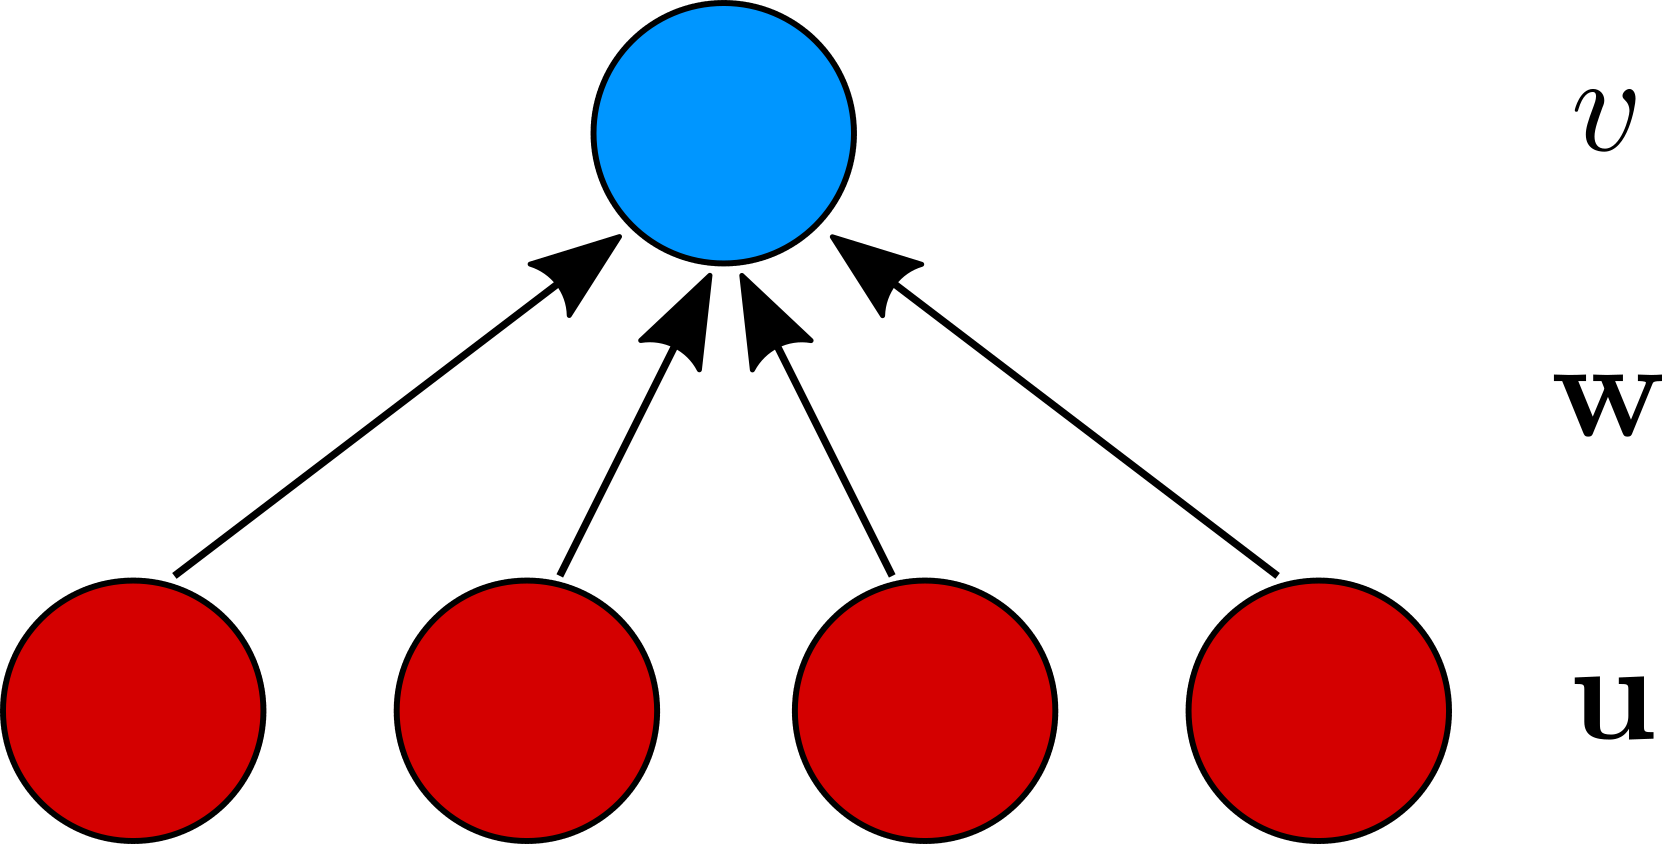
\includegraphics[width=0.5\columnwidth]{figures/single_neuron_input.png}
    \caption{Scheme representing a postsynaptic neuron (blue dot) being targeted by presynaptic neurons (red dots) through synaptic connections (black arrows). The synaptic weights of the connections are indicated with the vector $\mathbf{w}$, whereas the input rate is indicated with $\mathbf{u}$. The output of the postsynaptic neuron is indicated with $v$.}
    \label{fig:single_neuron_input}
\end{figure}

If we consider a exponential synaptic response, similarly to Equation \eqref{eq:cond_exp} but describing the synaptic current, we can write
\begin{equation}
    \label{eq:firing_rate_current}
    \tau_{\text{syn}}\dfrac{dI_{\text{syn}}}{dt}=-I_{\text{syn}}+\mathbf{w}\cdot\mathbf{u}
\end{equation}

Once the total input is evaluated, we have to estimate the response of the neuron through a \textit{activation function} $\mathcal{F}(I_{\text{syn}})$. Among the most common activation functions are the Heaviside step function $\mathcal{H}(x)$ and the threshold-linear (or ReLU)

\begin{equation}
\label{eq:ReLu}
\mathcal{F}(x) = \alpha \text{ max}\{ 0, x\}
\end{equation}

where $\alpha$ is a multiplicative coefficient.\\
Generally, in such a models, neurons do not respond instantaneously to the synaptic input, and thus the firing rate follows the linear differential equation

\begin{equation}
    \label{eq:firing_rate_I}
    \tau_{\nu}\dfrac{d\nu}{dt}=-\nu+\mathcal{F}(I_{\text{syn}})
\end{equation}
The time constant $\tau_{\nu}$ expresses the time needed for the neuron to reach a steady state firing rate when a constant input is given. Usually, in firing rate models, the time constant of the input current $\tau_{\text{syn}}$ is considered negligible with respect to $\tau_{\nu}$, and thus, for $\tau_{\text{syn}}\ll\tau_{\nu}$ Equation \eqref{eq:firing_rate_I} reduces to

\begin{equation}
    \label{eq:firing_rate}
    \tau_{\nu}\dfrac{d\nu}{dt}=-\nu+\mathcal{F}(\mathbf{w}\cdot\mathbf{u})
\end{equation}

Indeed, a network behavior can be described by these equations, and steady-state solutions can shed light on the long-term behavior of a network performing determined tasks, as we will see further in this work.\\
In this regard, we will present both feed-forward and recurrent networks, thus a brief introduction of how can such a networks can be described is provided following \cite{abbot2005}.\\
Figure \ref{fig:single_neuron_input} shows an example of feed-forward network, since the flow of the signals has only one direction, i.e., from the population below to the neuron above. Considering a population of postsynaptic neurons instead of having a single cell and calling $\mathbf{u}$ the rate of the population below (ergo the presynaptic one) and $\mathbf{v}$ the rate of the population above, we can write

\begin{equation}
    \label{eq:feed_forward}
    \tau_{\nu}\dfrac{d\mathbf{v}}{dt}=-\mathbf{v}+\mathbf{\mathcal{F} }(\mathbf{W}\cdot\mathbf{u})
\end{equation}

where $\mathbf{W}\cdot\mathbf{u}=\sum_{b=1}^{N_{u}}W_{ab}u_b$ for $a=1,\ldots,N_{v}$. Indeed, in case of feed-forward network the steady-state solution is totally similar to the one shown before, however, this is not true in case of recurrent network. In a recurrent network a neuron population can have self connections, and thus the output rate of the neurons depend on the rate of the population itself. Next figure shows a scheme of a recurrent network.

\begin{figure}[H]
    \centering
    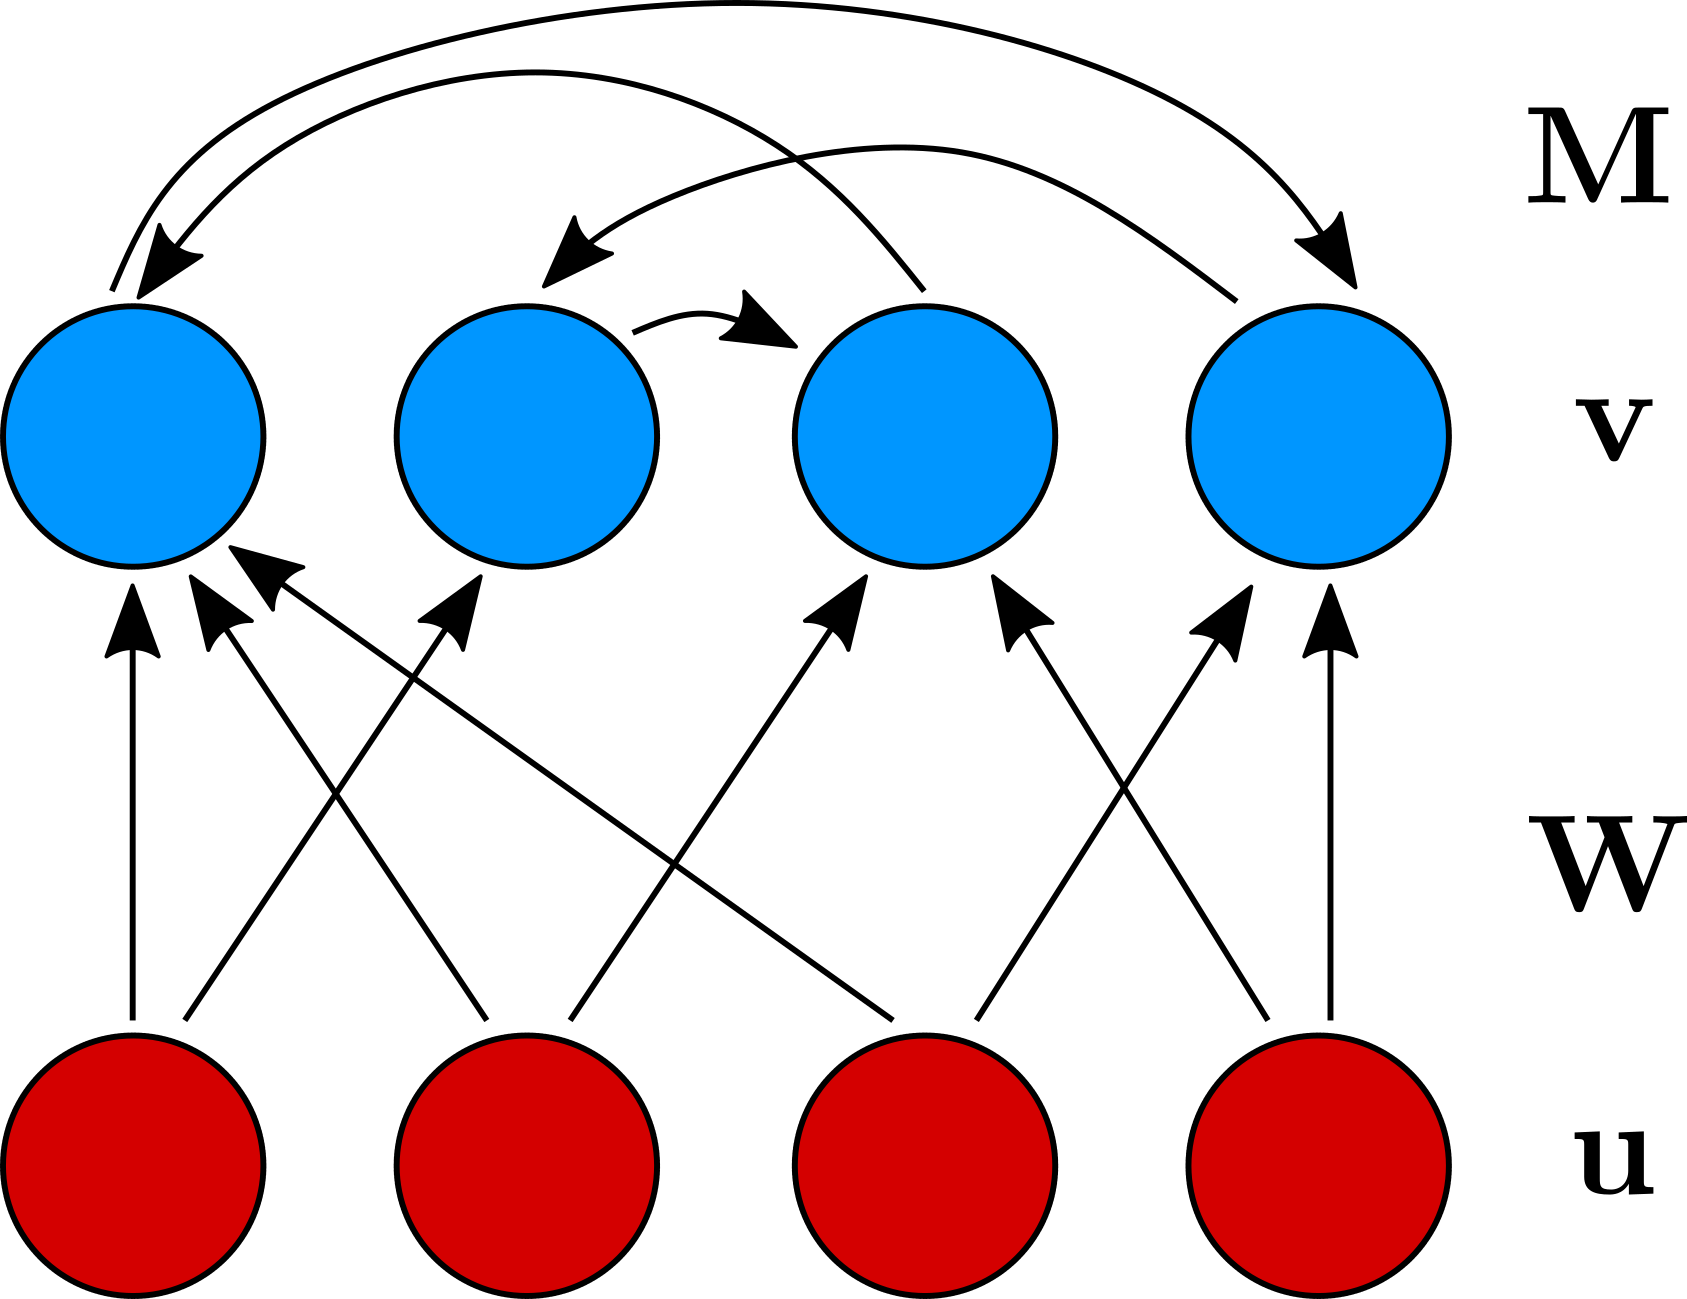
\includegraphics[width=0.5\columnwidth]{figures/recurrent_rate_model.png}
    \caption{Scheme of a recurrent network with two neuron populations. The synaptic weights of the feed-forward connections are indicated with the matrix $\mathbf{W}$, whereas $\mathbf{M}$ indicates the set of synaptic weights of the recurrent connections.}
    \label{fig:recurrent_network}
\end{figure}

 Calling $\mathbf{M}_{a,a'}$ the matrix which contains the synaptic weights from output neurons $a$ and $a'$, Equation \eqref{eq:feed_forward} becomes

\begin{equation}
    \label{eq:recurrent}
    \tau_{\nu}\dfrac{d\mathbf{v}}{dt}=-\mathbf{v}+\mathbf{\mathcal{F} }(\mathbf{W}\cdot\mathbf{u} + \mathbf{M}\cdot\mathbf{v})
\end{equation}

Indeed, the matrix $\mathbf{M}$ here considers only self connections of the output population, but it can be considered in a similar way also the contribution of a second population (e.g. an inhibitory one) which is stimulated by the output population and then projects to it an inhibitory feedback. Such an architecture is widely used when a realistic architecture of a neural circuit has to be represented, since the addition of an inhibitory population grants the stability of the excitatory (i.e. output) population and can also lead to mechanisms of competition through lateral inhibition that take place in the human brain.


\chapter{\textbf{Synaptic plasticity and cognitive processes}}
\label{chapter:intro_biology_synapses}

\begin{tcolorbox}[colback=white,colframe=DarkRed,title=\textbf{Summary}]
Here the synaptic models studied in compliance with this thesis are presented, i.e.,  short-term synaptic plasticity and structural plasticity. The description of these plasticity mechanisms is then followed by a discussion of the relationship between them and cognitive processes such as working memory and learning.
\end{tcolorbox}

\section{Short-term synaptic plasticity (STP)}
\label{sec:STP}
In this section short-term plasticity and its phenomenological description is introduced. For further details please see \cite{tsodyks1998, markram_wang_tsodyks1998, tsodyks2000, barak_tsodyks2007, Barri2022}.

Short-term plasticity (STP) is a mechanism in which the synaptic efficacy temporarily changes with a timescale on the order of hundreds or thousands of milliseconds. This phenomenon is regulated by the amount of synaptic resources (i.e. the neurotransmitters) available in the synapse at the moment of spike emission and by the calcium levels into the presynaptic terminal.

Indeed, the spike arrival to the presynaptic terminal elicits an influx of calcium ions that is responsible for the release of the vesicles in which neurotransmitters are stored. Higher calcium concentration into the terminal leads to a higher fraction of neurotransmitters released. This mechanism is called short-term facilitation (STF). The neurotransmitter release is then followed by a mechanism of calcium removal from the presynaptic terminal to restore its baseline concentration. 
The amount of neurotransmitters a synapse can contain is limited and the emission of a spike diminishes the number of neurotransmitters available in the presynaptic terminal for a further stimulation. This mechanism is called short-term depression (STD). Without synaptic activity, the amount of available neurotransmitters into the presynaptic terminal returns to its baseline level. 
The coupling of these two phenomena leads to a temporary modulation of the synaptic efficacy (i.e. short-term plasticity).

The first phenomenological model for short-term plasticity was presented in \cite{tsodyks1998}. The model describes mechanisms that take place in the presynaptic terminal, such as the neurotransmitter dynamics, taking into account the fact that neurotransmitters are limited and also the mechanism of neurotransmitter release is triggered by calcium ions. The neurotransmitter dynamics can be described by three normalized quantities that represent the fraction of neurotransmitters in three different states:
\begin{itemize}
    \item recovered ($x$), i.e., contained into synaptic vesicles, ready to be released;
    \item active ($y$), i.e., released in the synaptic cleft;
    \item inactive ($z$), i.e., in the process of returning inside the synaptic vesicles.
\end{itemize}
The mechanism related to calcium dynamics is described by a normalized quantity called $u$, which represents the fraction of opened calcium channels. Short-term plasticity can thus be described by the following set of equations:

\begin{equation}
    \label{eq:STP_tosdyks98}
    \begin{split}
    \dfrac{dx}{dt} &= \dfrac{z}{\tau_d} - u(t_s)x(t_s -\epsilon) \delta (t-t_s) \\
    \dfrac{dy}{dt} &= -\dfrac{y}{\tau_{\text{syn}}} + u(t_s)x(t_s-\epsilon) \delta (t-t_s) \\
    \dfrac{dz}{dt} &= \dfrac{y}{\tau_{\text{syn}}} - \dfrac{x}{\tau_{d}} \\
    \dfrac{du}{dt} &= -\dfrac{u}{\tau_f} + U(1-u)\delta (t-t_s)
    \end{split}
\end{equation}
Where $t_s$ is the time at which a spike is emitted, $\delta (\cdot)$ is a Dirac delta and $\tau_{\text{syn}}$, $\tau_f$ and $\tau_d$ are the synaptic time constant and the time constants for facilitation and depression mechanism, respectively.\\
Synaptic modulation is driven by the variable $y(t)$, ergo considering a synaptic efficacy $J$, the postsynaptic potential would have an amplitude of $Jy(t)$. In this equation, for simplicity, we neglect the indexed $i,j$ indicating the indexes of presynaptic and postsynaptic neuron. The quantity $u$ increases by a factor $U(1-u)$ whenever a presynaptic spike arrives, since the spike triggers the opening of calcium channels.\\
Is it possible to show that such a model can be simplified by adopting a system of two differential equations which describe the behavior of the synaptic resources ($x$) and the one of the utilization factor ($u$) \cite{tsodyks1998}. Let $x$ be the normalized amount of available resources into the presynaptic terminal and let $u$ be the fraction of resources used in a spike emission. The spike arrival to the synaptic terminal rises the variable $u$ by a quantity $U(1-u)$ (so that $u$ remains normalized) and the amount of resources released is equal to $ux$. Considering a synapse connecting the presynaptic neuron $i$ and the postsynaptic neuron $j$, this dynamics can be described by the following equations \cite{Mongillo2008}:
\begin{equation}
    \label{eq:STP}
    \begin{split}
    \dfrac{du_{i,j}}{dt} &= -\dfrac{u_{i,j} - U}{\tau_f} + U(1-u_{i,j})\sum_s\delta (t-t_s^{(i)}) \\
    \dfrac{dx_{i,j}}{dt} &= \dfrac{1-x_{i,j}}{\tau_d} - u_{i,j}x_{i,j} \sum_s\delta (t-t_s^{(i)})
    \end{split}
\end{equation}

where $\delta (\cdot)$ is the Dirac delta function and the sum is over the spike times $t_s^{(i)}$ of the presynaptic neuron $i$. The synaptic modulation takes place during the spike emission, so that
\begin{equation}
    J_{i,j}(t) = J^{\text{(abs)}}_{i,j}u_{i,j}(t-\hat{\delta}_{i,j})x_{i,j}(t-\hat{\delta}_{i,j})
    \label{eq:Jupdate}
\end{equation}
where $J^{(abs)}_{i,j}$ is the absolute synaptic efficacy for the synapse connecting neurons $i$ to neuron $j$ and $\hat{\delta}_{i,j}$ is the synaptic delay. Thus, when a spike is fired, the synaptic efficacy is described by the product $Jux$.\\

Short-term plasticity can show STD-dominated or STF-dominated behaviors depending on the choice of the time constants for the mechanism of depression and facilitation. The former can be observed when the mechanism of neurotransmitter restoration is slower with respect to the mechanism of residual calcium removal after spike emission and vice versa. To give a phenomenological description of STP we can define, as in Equation \eqref{eq:STP}, $\tau_d$ as the time constant of the process of neurotransmitter restoring and $\tau_f$ the time constant for calcium removal mechanism. Thus we can observe STD-dominated dynamics when $\tau_d > \tau_f$ and STF-dominated dynamics when $\tau_d < \tau_f$. The following figure shows an example of STD-dominated and STF-dominated dynamics, in which two postsynaptic neurons receive signals from a presynaptic neurons through synaptic connections with STP with different facilitation and depressions time constants.


As can be seen, the neuron connected with the STF-dominated synapse is able to show a change in the postsynaptic potential after a relatively long period of time (around one second). This is achieved by the fact that the synaptic resources ($x$) can return quickly to the presynaptic terminal, whereas the calcium concentration in the terminal ($u$) decrease slowly. Since the STP modulation is driven by the factor $ux$, this results in a temporary potentiation of the synaptic efficacy. The STD-dominated synapse has the opposite effect, according to which the efficacy strongly decreases when a series of spikes has to be transmitted and slowly returns to the baseline efficacy.

\begin{figure}[H]
    \centering
    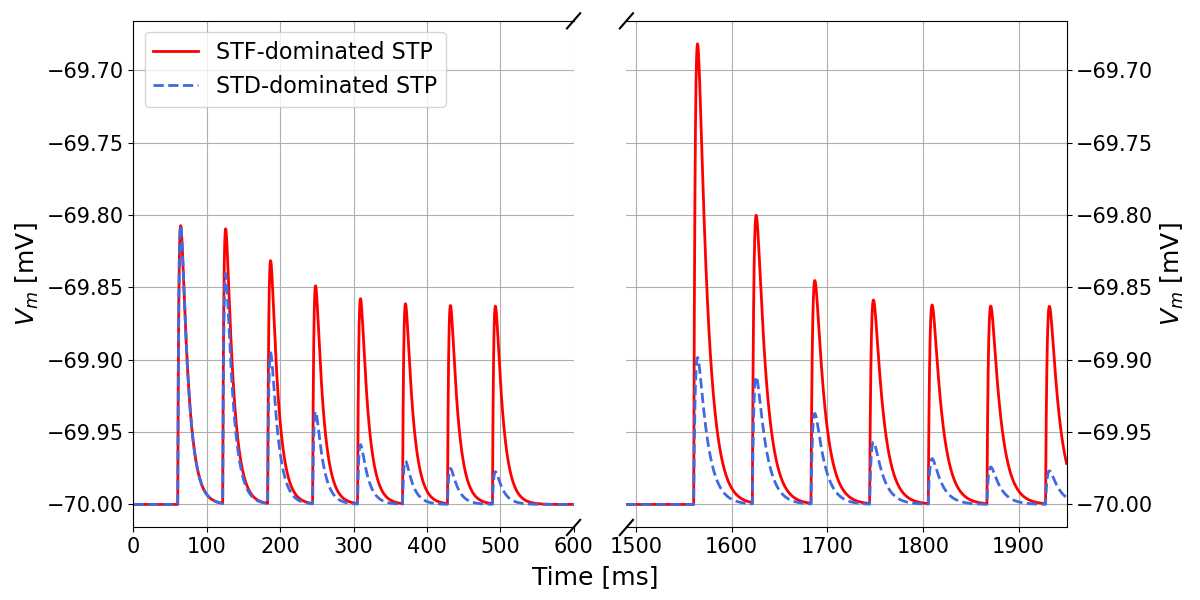
\includegraphics[width=\columnwidth]{figures/STP-sample.png}
    \caption{Voltage trace of two neurons connected with the same presynaptic neuron with a STP connection. A neuron has a STF-dominated connection (red line), with $\tau_f=1.5$\,s and $\tau_d=0.2$\,s, whereas the other neuron shows a STD-dominated behavior (blue-dotted line), with $\tau_f=0.2$\,s and $\tau_d=1.5$\,s. The time axis is interrupted between $600$ and $1500$\,ms, during which the presynaptic neuron is not active.}
    \label{fig:STPsample}
\end{figure}

\subsection{STP and Working Memory}
\label{sec:stp_wm}
We notice in Figure \ref{fig:STPsample} that facilitated (i.e., STF-dominated) synapses can show, after a relatively long time of inactivity, an increase in the synaptic efficacy. Indeed, it has been estimated that, in our brain, certain regions show a predominance of facilitated synapses, whereas many others show mostly STD-dominated synapses. Among the regions with more relevant occurrence of facilitated synapses we have the prefrontal cortex (PFC), which is believed to be one of the most important locations of the brain in which Working Memory (WM), that will be briefly introduced here, takes place. The question that arises is whether a synaptic mechanism such STP, and in particular synaptic facilitation, would be a synaptic correlate of working memory.


Working Memory is a cognitive process able to hold and manipulate information for a short time. It is involved in a vast number of cognitive tasks \cite{Miller1960, baddeley_hitch1974, Cowan1998, Golosio2015} which span from speech to visual and spatial processing. Differently from long-term memory, working memory is a transient phenomenon and it is also believed that it does not entail structural changes to the network.\\
A classic procedure for studying working memory relies on the so-called delay response tasks. In such a framework, a stimulus is presented for a short time and the related execution of the task can take place only after a delay period. During the delay period it is experimentally observed, especially in the prefrontal cortex, a neuronal selective persistent spiking activity able to maintain the information previously presented by the stimulus \cite{Funahashi1989, GoldmanRakic1995, DEsposito2015}. When this activity is somehow suspended (e.g. because of a noise stimulus during the delay period or a too long delay) the task is not correctly executed.\\
The first computational models assumed that this peculiar activity could be entirely maintained with prior long-term synaptic modifications so that, when a stimulus was given into the network, the population encoding for the presented stimulus exhibited a persistent spiking activity \cite{hebb-organization-of-behavior-1949, Hopfield1982}. Thus, according to these models, the information was only stored in the spiking activity. However, experimental evidences show that memory can be also maintained when the enhanced activity is interrupted, suggesting that information is not only stored in the populations spiking activity \cite{Stokes2015} and also that working memory processes can exhibit discrete periodic bursts instead of a persistent activity \cite{Honkanen2014, Lundqvist2016}.\\
In this framework many studies were conducted to enlighten the role of synaptic plasticity in working memory \cite{Barak2014} and some of the proposed models relies on short-term synaptic facilitation \cite{barak_tsodyks2007,Mongillo2008,Rolls2013,Hansel2013}. The work of \cite{Rolls2013} shows that employing synaptic facilitation enables a spiking network to maintain a relevant number of memories at the same time, whereas the same network lacking this kind of plasticity can maintain many fewer memories. Moreover, \cite{Hansel2013} argues that the non-linearity of short term facilitation is essential for displaying a reasonable persistent activity able to retain a memory during a delay period. \\
One of the models that posit a dominant role of synaptic facilitation in working memory is the one of \cite{Mongillo2008}, which shows that a spiking network with synaptic facilitation is able to exhibit a bi-stable regime in which it can autonomously retain memories with periodic spiking activity without a significant firing rate increase. Thus, according to this model, memories are stored in a synaptic fashion, with spiking activity functional for synaptic facilitation upkeep. The model is further employed in \cite{mi_katkov_tsodyks2017} to study how working memory capacity can be modulated by synaptic facilitation and network's external excitation.\\
More recently, \cite{Fiebig2017} (see also \cite{Fiebig2020}) proposed a spiking network model based on a fast expression of Hebbian plasticity, in which memory is retained by oscillatory bursts. Here, the authors proposed a synaptic plasticity model based on a Hebbian learning rule flanked by a short-term plasticity mechanism. This kind of implementation can enable a network to learn new memory representations, whereas using non-Hebbian plasticity needs a prior long-term network training.\\
In the context of this thesis we focused on the theory proposed by \cite{Mongillo2008}, first reproducing the results of the work using the spiking network simulator NEST \cite{Tiddia2022_WM} and then evaluating the model itself, to shed light on the limitations and the strength of such approach when comparing it to other working memory models that rely on different neural mechanisms. This study is presented in Chapter \ref{chapter:STP_WM_model}.

\section{Spike timing-dependent synaptic plasticity (STDP)}
The mechanisms involved in the modification of the synaptic efficacy of a synapse are many and take place at different time scale. As we noticed in the previous section, STP has a time scale of the order of seconds, and it only depends on the emission of a spike from the presynaptic terminal. Such a process is not related to an activity-driven potentiation of the synapses, which is believed to be a key process for learning according to the Hebb postulate \cite{hebb-organization-of-behavior-1949}, which states that there should be a metabolic process triggered by a repetitive and persistent firing from a presynaptic neuron to a postsynaptic one able to increase the efficacy of the signals transmitted.\\
In this regard, spike timing-dependent plasticity (STDP) is a mechanism that changes the synaptic efficacy of a synapse based on the times at which the presynaptic and the postsynaptic neurons emit a spike. In particular, when the presynaptic neuron fires slightly before the postsynaptic neuron, the synaptic efficacy increases following a long-term potentiation (LTP) process. This is related to the fact that between these events there could be a causal relation, and after repeated events in which presynaptic spikes are followed by postsynaptic activity some metabolic processes are triggered leading to a strengthening of the synaptic efficacy. On the contrary, a synapse that connects neurons that do not show this behavior can decrease its synaptic efficacy, leading thus to long-term depression (LTD).\\
The general behavior of STDP can be described by the following \cite{Morrison2008, Sjostrom2010}, given $\Delta t=t_j^f-t_i^f$ the spike times difference between the postsynaptic neuron $j$ and the presynaptic neuron $i$

\begin{equation}
\begin{cases}
\Delta \omega^+=F_+(\omega) e^{-|\Delta t|/\tau_+} & \text{if $\Delta t>0$}\\
\Delta \omega^-=F_-(\omega) e^{-|\Delta t|/\tau_-} & \text{if $\Delta t \leq 0$}
\end{cases}
\label{eq:stdp_simple}
\end{equation}

where $\omega$ represents the synaptic efficacy and $F(\omega)$ is a non time dependent function. Indeed, the only part of the equation that is time dependent is represented by the exponential functions, each one provided with a specific time constant, meaning that this rule is asymmetric with respect to $\Delta t$ (it is a form of Temporal Asymmetric Hebbian learning).


In 1968 the work of \cite{Bi1998} measured the synaptic modifications on neurons of the hippocampus, showing that the spike timing between the presynaptic and postsynaptic neuron determined "the direction and the extent of synaptic changes". Figure \ref{fig:stdp_bi_poo} shows the experimental results measured in that work.


The figure shows that there is an exponential dependence of the change in EPSC with respect to the spike timing. Further, a positive or negative $\Delta t$ determines an increase or a decrease of the postsynaptic current amplitude, respectively, and a different time constant for the time-dependent exponential behavior, as also reported in Equation \eqref{eq:stdp_simple}. STDP is here presented as a single phenomenological model, however several STDP models have been developed in recent times to take into account the several experimental observations regarding the role of the spike timing in long-term plasticity mechanisms (see \cite{Morrison2008} for a review).


\begin{figure}[H]
    \centering
    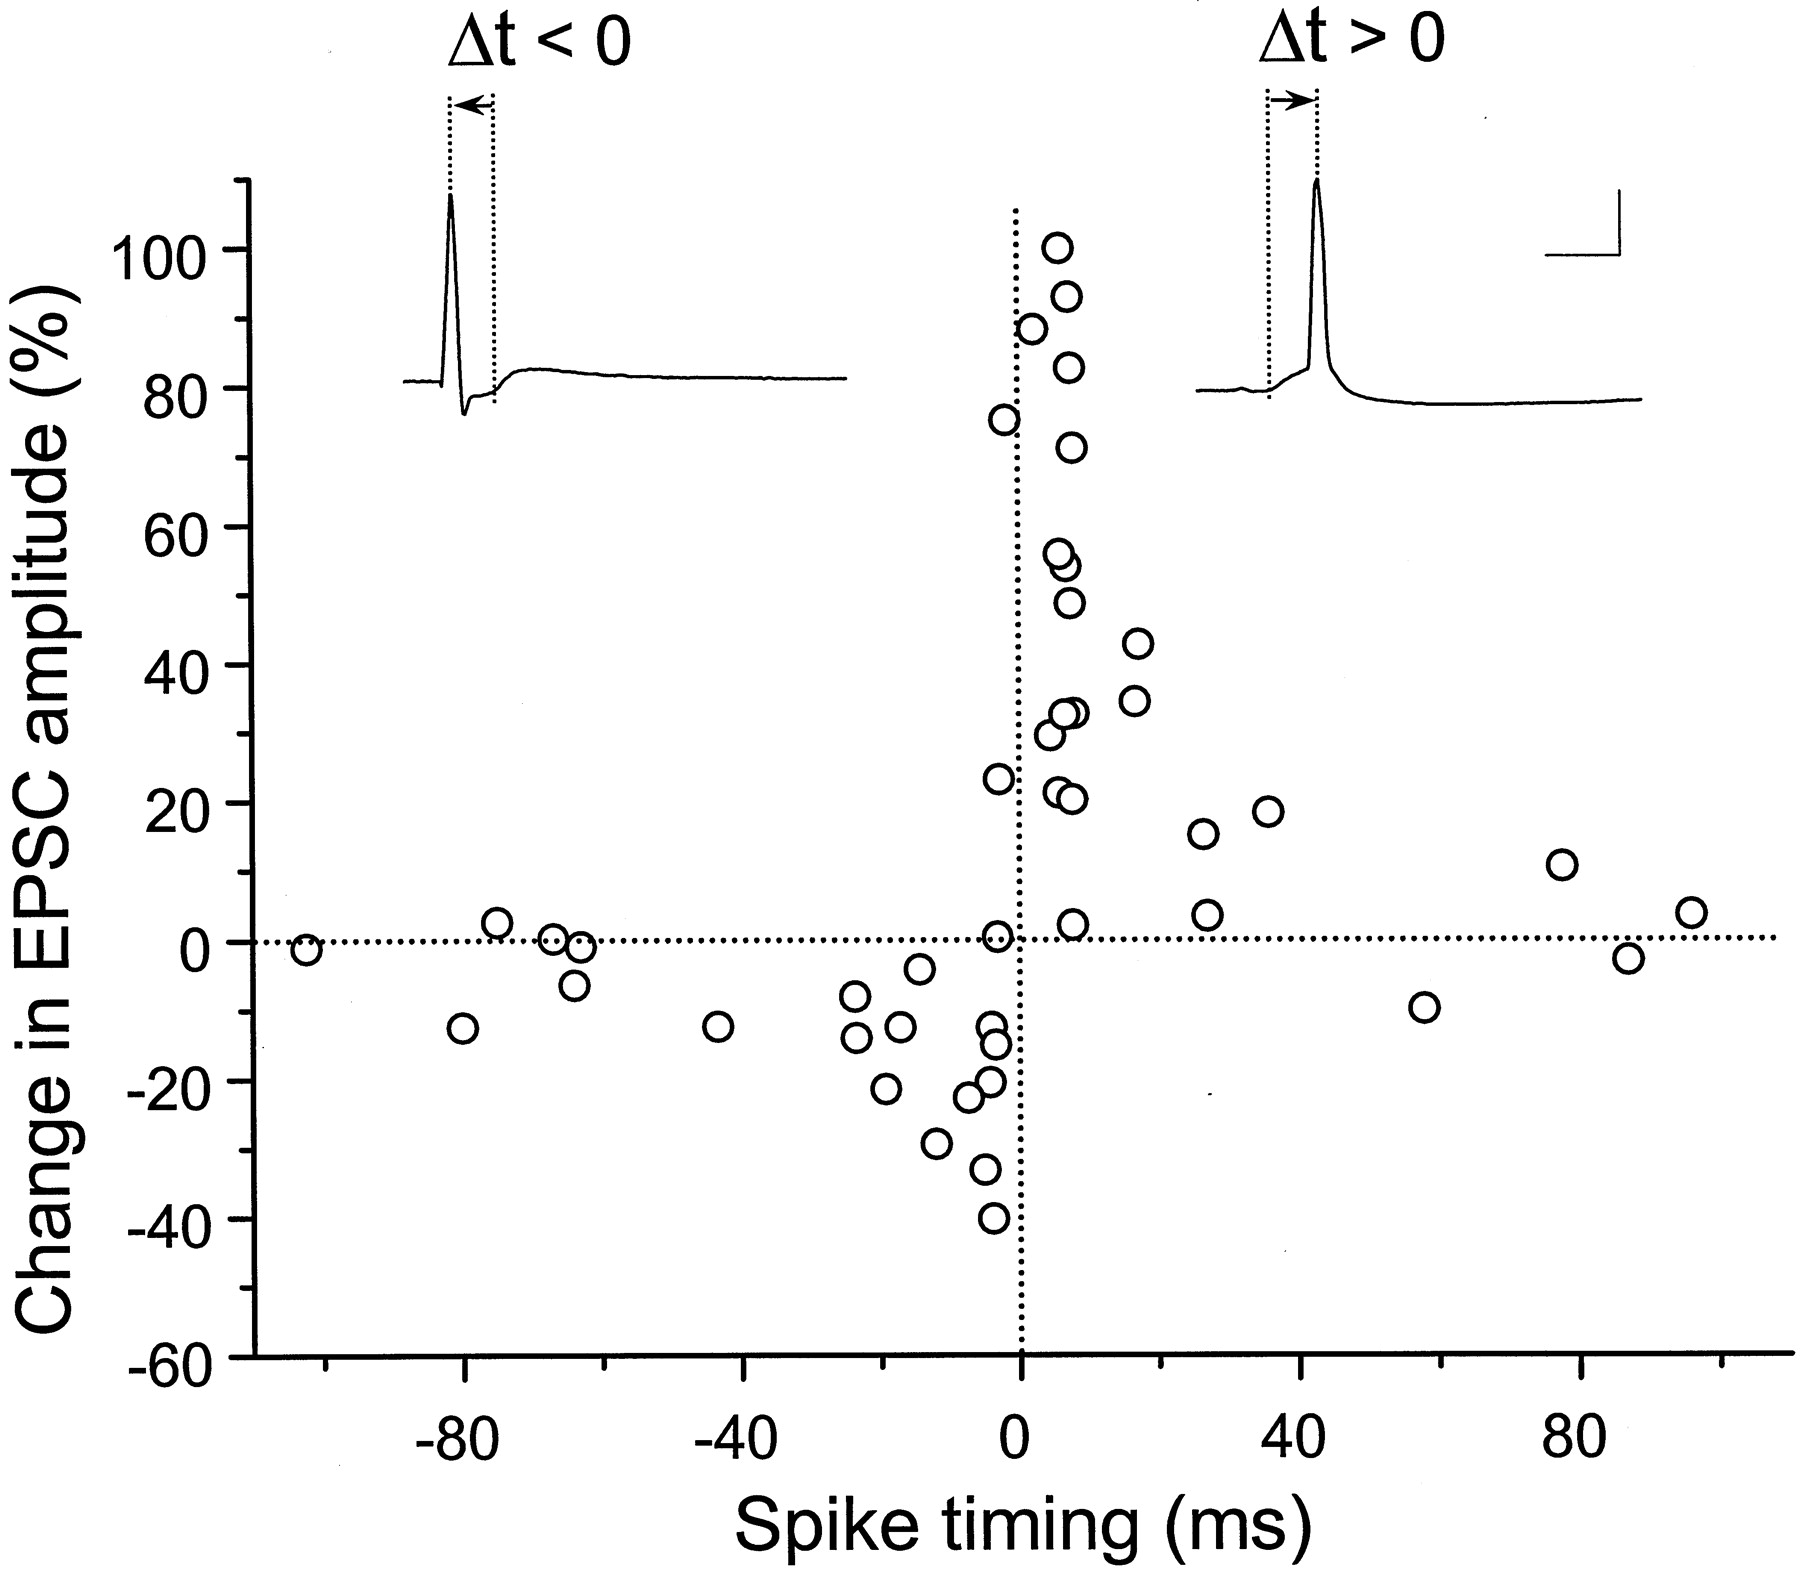
\includegraphics[width=0.6\columnwidth]{figures/stdp_bi_poo.jpg}
    \caption{Experimental measurements of synaptic potentiation and depression depending on the spike timing. The difference in the excitatory postsynaptic current amplitude (EPSC) is measured after repetitive correlated spiking activity. Spike timing is defined as the time difference between the beginning of the postsynaptic potential and the arrival of the presynaptic spike on the axonal terminal. Figure from \cite{Bi1998}.}
    \label{fig:stdp_bi_poo}
\end{figure}

\section{Structural plasticity and learning}
\label{sec:str_pl_and_learning}
While in the previous sections we discussed temporary and reversible changes of the synaptic efficacy of an instantiated synapse, here we discuss the structural changes in the synaptic morphology of the brain neuronal network, which takes place during all the life-time, constantly changing the architecture of our brain.\\
These changes occurs at longer time scales than the short or long-term mechanisms mentioned above, and consist in the consolidation, creation of new synapses or erasure of synapses that have not been consolidated. This kind of plasticity is called \textit{structural plasticity}. It can be spontaneous, but also activity-based \cite{Butz2009}, and it has a key role in the stabilization of new concepts that have to be kept in memory after learning \cite{Fu2011}.\\
Structural plasticity is underlain by several biochemical and biophysical mechanisms and, according to \cite{Fauth2016}, we can distinguish between two main categories: \textit{activity-dependent} and \textit{homeostatic} structural plasticity.\\
Activity-dependent structural plasticity (\textit{Hebbian} in \cite{Fauth2016}) is related to growth or retraction of neurites and formation of new synapses to increase the connectivity between two neurons with high and correlated activity, but also to deletion of synapses which connect neurons with low and uncorrelated activity. It is known that LTP induced by a strong neural activation is followed by an increase of the number of synapses. Moreover, LTP causes growth of dendritic spines, which is related to the efficacy of the synapses. The growth of a dendritic spine is associated to its stability in a way that a grown spine, to which corresponds a higher synaptic efficacy, is more stable, i.e. it is not likely to be removed. Thus, synaptic efficacy can somehow be related to structural plasticity and the probability for a synapse to be consolidated or removed \cite{Kasai2003, Hill2013}. Accordingly, it is also shown in several studies (see, for example, \cite{Toni1999}) that inhibiting LTP prevents the increase of the number of dendritic spines, corroborating the link between LTP, structural plasticity and synaptic efficacy changes in previously instantiated synapses. On the other hand, LTD too is linked to structural plasticity, showing that it leads to a reduction in the number of synapses \cite{Wiegert2013}.\\
These activity dependent modifications are then flanked by an homeostatic kind of structural plasticity, which consist in a decrease in connectivity between neurons with high neuronal activities and an increase within neurons with low activity. Thus, this mechanisms results in a balancing effect that, through dendritic and axonal modifications, leads to a regime of intermediate postsynaptic neuronal activity 
(see \cite{Butz2009} for a review). These effects are summarized in Figure \ref{fig:str_pl_effects}.\\

\begin{figure}[ht]
    \centering
    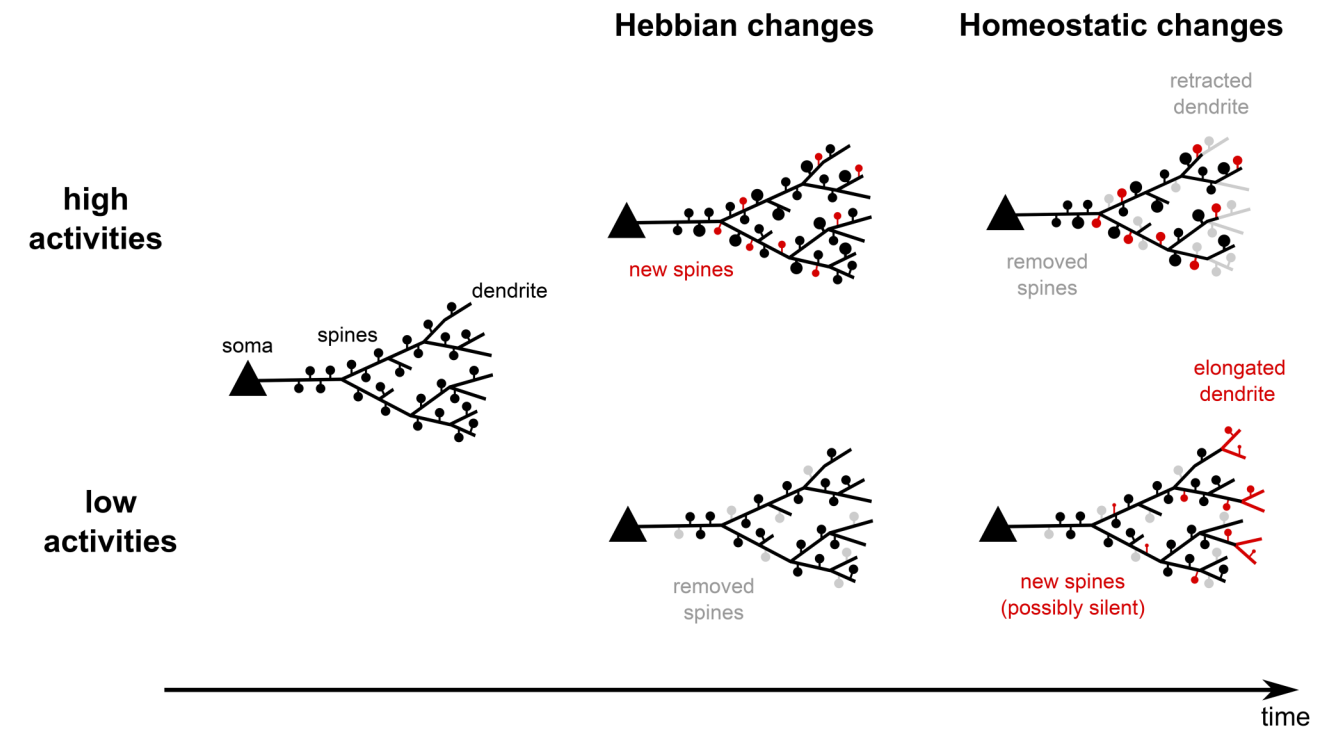
\includegraphics[width=\columnwidth]{figures/summary_str_pl.png}
    \caption{Summary of the effects of activity-dependent (i.e. Hebbian) and homeostatic structural plasticity when having high or low neuronal activity. In case of high activity, new dendritic spines are formed following the Hebbian mechanisms and, to maintain the homeostasis some connections are removed afterwards. An opposite behavior can be seen for low neuronal activity. Figure from \cite{Fauth2016}.}
    \label{fig:str_pl_effects}
\end{figure}

In addition, the number of synapses in the brain can change over time. In \cite{Huttenlocher1979} it is shown that synaptic density reaches the highest values at $1$-$2$ years age, it drops during adolescence and stabilizes between age $16$-$72$, followed by a slight decline. However, although synaptic density remains approximately stable during adulthood, rewiring of network connections occurs as well. Indeed, the increase of connections in high activity regions (and vice versa), together with the rearrangement of synapses leads to a fine-tuning of the brain's circuits \cite{sakai2020}, because on one hand some synapses are strengthened through long-term potentiation (LTP) and new connections are formed next to the already potentiated ones to further enhance synaptic transmission, on the other hand when the presynaptic and postsynaptic neuron activities have low correlation their connection are likely to be removed. Indeed, synaptic pruning is considered essential for optimizing activity propagation and memory capacity \cite{Chklovskii2004, Knoblauch2014, Knoblauch2016}.
Additionally, it is commonly believed that synaptic pruning and rewiring dysfunction are among the neural correlates of developmental disorders such as autism or schizophrenia \cite{Bourgeron2009,Moyer2015}, leading to a higher or lower synaptic density with respect to neurotypical subjects, respectively\cite{Hutsler2010,Pagani2021,Glantz2000}.\\
Only in recent times, computational models of structural plasticity and connectivity rearrangements during learning were developed, showing intriguing results. \cite{Knoblauch2014} and \cite{Knoblauch2016} describe a model of structural plasticity based on "effectual connectivity", defined in these works as the fraction of synapses able to represent a memory stored in a network. By structural plasticity, effectual connectivity is improved, since synapses that do not code for the memory are moved in order to optimize network's connectivity. Their model defines synapses using a Markov model of three states: potential (i.e. not instantiated), instantiated but silent or instantiated and consolidated. Structural plasticity is thus related to the passage of the synapses from a potential state to an instantiated state (and vice versa), whereas changes only related to the synaptic weight are described by the consolidation of the instantiated synapses. With such a model, it is possible to show that networks with structural plasticity have higher or comparable memory capacity to networks with dense connectivity and it is possible to explain some cognitive mechanism such as the spacing effect \cite{Knoblauch2014}.\\
\cite{Spiess2016} simulated a spiking neural network with structural plasticity and STDP, showing that structural plasticity reduces the amount of noise of the network after a learning process, thus making the network able to have a clearer output. Furthermore, such a network with structural plasticity shows higher learning speed than the same network with only STDP implemented.\\
Some new insights about the importance of synaptic pruning are also shown in \cite{Navlakha2015}, in which different pruning rates were studied suggesting that a slowly decreasing rate of pruning over time leads to more efficient network architectures.\\
Chapters \ref{chapter:structural_plasticity_theory} and \ref{chapter:structural_plasticity_simulation} of this thesis will expand this discussion proposing a new theoretical model for learning through structural plasticity supported by firing-rate-based simulations. The model is designed to consider the effects of both activity-dependent and homeostatic structural plasticity as described in this section, and can help shading light on the role of structural modifications of brain circuits during learning.


\part{GPU-based simulations of spiking networks}
\label{part:I}

\chapter{\textbf{Simulation technology: CPU, GPU-based and beyond}}
\label{chapter:intro_simulators}

\begin{tcolorbox}[colback=white,colframe=DarkRed,title=\textbf{Summary}]
This chapter introduces some spiking network simulators, with particular regard to NEST GPU, i.e., the GPU version of the NEST simulator. After presenting the currently most used simulators, classified according to the type of hardware that supports them, the dissertation will focus on GPU computing and NEST GPU accompanied by the description of some of its algorithms.
\end{tcolorbox}

\section{From CPUs to GPUs and neuromorphic computing: a brief introduction}
Spiking neural networks are used to study the behavior of neuron populations with single neuron resolution. They are establishing themselves as a flexible and powerful tool to study the brain function resulting from neuronal dynamics. Moreover, the development of the simulation technology is leading to more complex and realistic network architecture being able to simulate the dynamics of large networks of neurons more accurately and more efficiently in terms of performance.\\
Currently, the simulation of spiking neural network can greatly benefit from a large variety of hardware: from conventional hardware like CPUs and GPUs to chips specifically designed for this kind of computation, such as FPGA and neuromorphic hardware. On a software perspective, in the last decades many simulators have been developed to provide the neuroscientific community with powerful yet flexible and intuitive platforms to simplify the simulations of such networks and produce good quality data. Indeed, the development of simulation software able to take advantage of the most recent computing technology is vital for paving the way for more detailed and realistic models. For this reason, many simulation software have recently introduced different back-ends in order to benefit from the largest variety of hardware.\\
Among the most established spiking network simulators we can mention NEST \cite{Gewaltig2007}, NEURON \cite{Carnevale_2006}, Brian 2 \cite{Stimberg2019} and ANNarchy \cite{Vitay2015}. 
These simulators are capable of simulating a large variety of neuron and synapse models and support multi-thread parallel execution on general-purpose CPU-based systems. In addition, NEST and NEURON support distributed computing via MPI.\\
Neuromorphic hardware is an umbrella term for research oriented towards brain-inspired hardware architectures. In this regard, many projects have been developed; we can mention Loihi \cite{Loihi2018} and TrueNorth \cite{TrueNorth2015}, which are entering the realm of large-scale neural network simulations, and BrainScaleS \cite{Grbl2020}, which is based on analog emulations of simplified models of spiking neurons and synapses, with digital connectivity. The system enables energy-efficient neuronal network simulations, offering highly accelerated operations. Another promising project in this field is SpiNNaker \cite{Furber2014}, which recently achieved biological real-time simulations of a cortical microcircuit model \cite{Rhodes2020} proposed by \cite{Potjans2012}. This model has since been simulated sub-realtime with NEST \cite{Kurth2022}, on FPGA-based neural supercomputer \cite{Heittmann2022, Kauth2023} and also with NEST GPU \cite{Golosio2023}, as will be discussed later.
SpiNNaker's result was made possible by its architecture designed for efficient spike communication, performed with an optimized transmission system of small data packets. BrainScaleS and SpiNNaker are freely available to the scientific community through the EBRAINS Neuromorphic Computing service.\\
Nevertheless, neuromorphic systems still require a significant amount of system-specific skills. Even if the simulation speed they can provide is impressive, the flexibility and simplicity of programming environments available for such neuromorphic systems are still low compared to their general-purpose counterparts. On neuromorphic systems adopting analog design techniques, advantages in speed, area, and energy consumption are associated with the difficulties of managing manufacturing fluctuations, unavoidable in analog substrates, and with the effects of electronic noise emerging in the dynamics of analog circuits. Porting neural simulations from digital systems to analog neuromorphic platforms is not a trivial task. Overcoming such difficulties and turning them into advantages is an emerging field of research \cite{Wunderlich2019}. Furthermore, as soon as the number of synapses per neuron reaches biological scales (i.e., several thousands per neuron), the current generation of neuromorphic systems can experience significant slowdown. For example, in its maximum configuration, the first-generation BrainScaleS system hosts 1 billion synapses and 4 million neurons (250 synapses per neuron) on 20 silicon wafers \cite{Guttler2017}, and a similar synapse-per-neuron ratio is the sweet spot for optimal execution on SpiNNaker, well below the typical $10,000$ synapses per neuron characteristic for pyramidal cortical neurons. However, FPGA-based cluster recently show promising results in the simulation of the cortical microcircuit model of \cite{Potjans2012}, being around $20\times$ faster than realtime in a network with natural density, paving the way for a new generation of neuromorphic system that will have to simulate even larger scale networks \cite{Kauth2023}.\\
Now, after having introduced simulators that employ CPUs or specific neuromorphic chip, GPU-based simulators will be presented.

\subsection{GPU-based simulation}
Over the past years, the use of GPUs (Graphical Processing Units) for parallel computing had a significant surge in  popularity across various research fields, from scientific simulation, to data analysis, deep learning and machine learning in general. Indeed, this hardware is provided with thousands of cores executing multiple threads simultaneously, resulting in an hardware capable of a very high degree of parallelism. Types of computation based on SIMD parallelism (i.e., Single Instruction Multiple Data) can largely benefit from GPUs parallelism. For this reason, GPU manufactures developed specific frameworks such as CUDA or OpenCL to take full advantage of the GPU capabilities. Moreover, GPUs are becoming more and more affordable and can be easily found in the consumer market, even inside high-end laptops.
Supercomputers are also taking advantage of the GPU availability, since they are reaching for exascale by drawing a significant portion of their compute power from GPUs.\\
For neuroscience to benefit from these systems, efficient GPU-based back-end for neural network simulators have been developed. For instance, simulation codes such as ANNarchy, NENGO \cite{Bekolay2014}, Arbor \cite{paper:arbor2019}, and CARLsim \cite{CARLsim6} provide a GPU back-end. Moreover, simulators such as Brian and NEURON have simulation codes that take advantage of GPUs, i.e., Brian2CUDA \cite{Alevi2022} and CoreNEURON \cite{Kumbhar2019} respectively.\\
However, there are simulators such as GeNN \cite{Yavuz2016}, or the previously mentioned CARLsim, that are primarily designed for GPUs, with CUDA \cite{sanders10} being the most widely used scripting language for the device code (ergo NVIDIA GPUs are employed) and \verb!C!/\verb!C++! for host code. Among GPU-based simulators we can say that GeNN is currently one of the most popular. Integrated also in the Brian simulator as Brian2GeNN \cite{Stimberg2020}, GeNN was able to outperform CPU-based and neuromorphic code in the simulation of a highly-connected large scale network \cite{Knight2018} and recently managed to simulate a multi-area spiking network model \cite{Schuecker2017, Schmidt2018b, Schmidt2018} on a single GPU card \cite{Knight2021b}. This result was achieved with the procedural connectivity approach, consisting in generating the model connectivity and its synaptic weights only when spikes need to be transmitted, without storing any connectivity data in the GPU memory. Nonetheless, such an approach can be efficient from a memory point of view, since one of the most constraining features of GPUs is the size of the built-in memory, which in spiking neural network simulations can be a severe limitation. However, this method can be suitable only with static synapses, since plastic synapses require a storage of the synaptic weights, which change their value during the simulation.\\
One interesting topic for spiking network simulation codes, no matter the back-end, is the way a network is instantiated and prepared for the simulation. Indeed, every simulation code employs different solutions, with algorithms that are adapted to the type of simulation hardware the simulator takes advantage from. From now on, we will call this task \textit{network construction}. Generally speaking, we can identify two macro-categories of network construction management:

\begin{itemize}
    \item network construction during runtime using scripting languages;
    \item code-generation approaches, which require the code to be firstly generated through a high-level description provided by the user before it is compiled and executed.
\end{itemize}

On one hand, code-generation approaches offer an advantage since, after code-generation and compilation, the time for model construction is generally negligible. On the other hand, a new compilation is needed whenever there is a modification of the model to be applied, with times needed for this task typically much longer than network construction times \cite{Golosio2020}. Runtime network construction network can offer more ease in model implementation, and can be also an advantage in some contexts like parameter scan applications. However, they can be less performing than code-generation approaches \cite{Golosio2021}.\\
Hitherto we presented a plethora of simulation codes, lastly focusing on GPU-based codes. Now the GPU-based simulation code NEST GPU will be introduced.

\section{NEST GPU}
NEST GPU \cite{Tiddia2022}, previously named NeuronGPU \cite{Golosio2021}, is a GPU library for simulation of large-scale networks of spiking neurons. Written in \verb!CUDA!-\verb!C++!, it is provided with a Python interface, with most commands being similar, if not identical, to the Python interface of the NEST simulator. Indeed, it has been recently included into the NEST Initiative with the aim of integrating it with the NEST simulator to allow for GPU-based simulations. To open for large-scale simulations of spiking networks, it is able to exploit multiple GPUs on MPI clusters. In this regard, NEST GPU implements a novel MPI-optimized spike delivery algorithm that has been tested on a MPI-GPU cluster in \cite{Tiddia2022} on the simulation of the multi-area model of \cite{Schuecker2017, Schmidt2018b, Schmidt2018}. One of the greatest advantages for the simulations of such a models is the algorithm used for the neuron distribution among the different MPI processes. Indeed, NEST GPU exploits the neuron distribution described in \cite{Pastorelli2019}, according to which the spacial locality of the neurons is taken into account. To be more specific, this means that neurons belonging to the same population (or cortical circuit in general) are simulated in the same MPI process. This is a potentially great advantage, since intra-population connections are generally higher in number that inter-population connections. Thus, this approach leads to a limited load on MPI communication with respect to other algorithms. For example, one of the most utilized approaches for neuron distribution in MPI simulations is the round-robin, for which neurons are evenly distributed across the MPI processes, meaning that in each MPI processes there are neurons belonging to every neuron population simulated. This approach grants an optimal load balance across MPI processes, but can be less efficient depending on the network architecture since it can lead to a much higher compute load on MPI communication.\\
Regarding the network construction, NEST GPU fall in the category in which the network is built on runtime. In previous versions of NEST GPU (see for example the prototype library NeuronGPU \cite{Golosio2021}), the network construction process was not handled by the GPU, but the network was built in the CPU. However, the network had to be transferred from CPU to GPU for the simulation of the network dynamics to start. This copy operation between RAM and GPU memory was indeed a bottleneck for the network construction, which resulted comparable or even slower than CPU-based simulator such as NEST \cite{Golosio2021, Tiddia2022}. Even if the network construction time is a fixed overhead with respect to the time-to-solution, a relatively slow network construction approach can limit the efficiency of application such as parameter scan, where several simulations have to be done, resulting in a significant contribution to the overall execution time. For this reason, we came up with a novel algorithm for dynamic network construction directly in the GPU devices that is able to reach state-of-art performance for network construction \cite{Golosio2023}. The following subsections give a brief description of the spike delivery and communication algorithm and the novel network construction algorithm.

\subsection{Spike delivery algorithm}
Spike delivery algorithms can be significantly different among different simulation code, mainly depending on the hardware the simulators use. NEST GPU exploits a specific spike delivery algorithm, which is here briefly introduced. For a more detailed description, please refer to \cite{Golosio2021, Tiddia2022}.\\
In NEST GPU, each neuron is provided with an output spike buffer, which holds the spikes emitted by the neuron. Output connections of the neuron are organized in groups, with each group collecting connections with the same synaptic delay. Each spike is identified by three values:
\begin{itemize}
    \item multiplicity, i.e., an integer that indicates how many spikes correspond to the spike event in exam. Generally, this value is $1$, but can be greater in case, for example, of spiking devices with Poisson statistics;
    \item time index $t_{\text{s}}$, which starts from $0$ and is increased by $1$ at every simulation time step;
    \item connection-group index $i_{\text{g}}$, which starts from $0$ and is incremented every time the time index matches a connection-group delay.
\end{itemize}

Given these values for each spike event, the spike is sent when the time index of the spike $t_{\text{s}}$ matches a connection-group delay. This way, the spike is sent in that simulation time step to all the target nodes of the connection group associated to the matching delay. In particular, when a spike has to be transmitted, it is firstly sent to a spike array. Finally, the spike is sent from this array to the target neurons using a CUDA kernel. Figure \ref{fig:spike_delivery_algorithm} depicts the workflow of the spike buffer.

\begin{figure}[H]
    \centering
    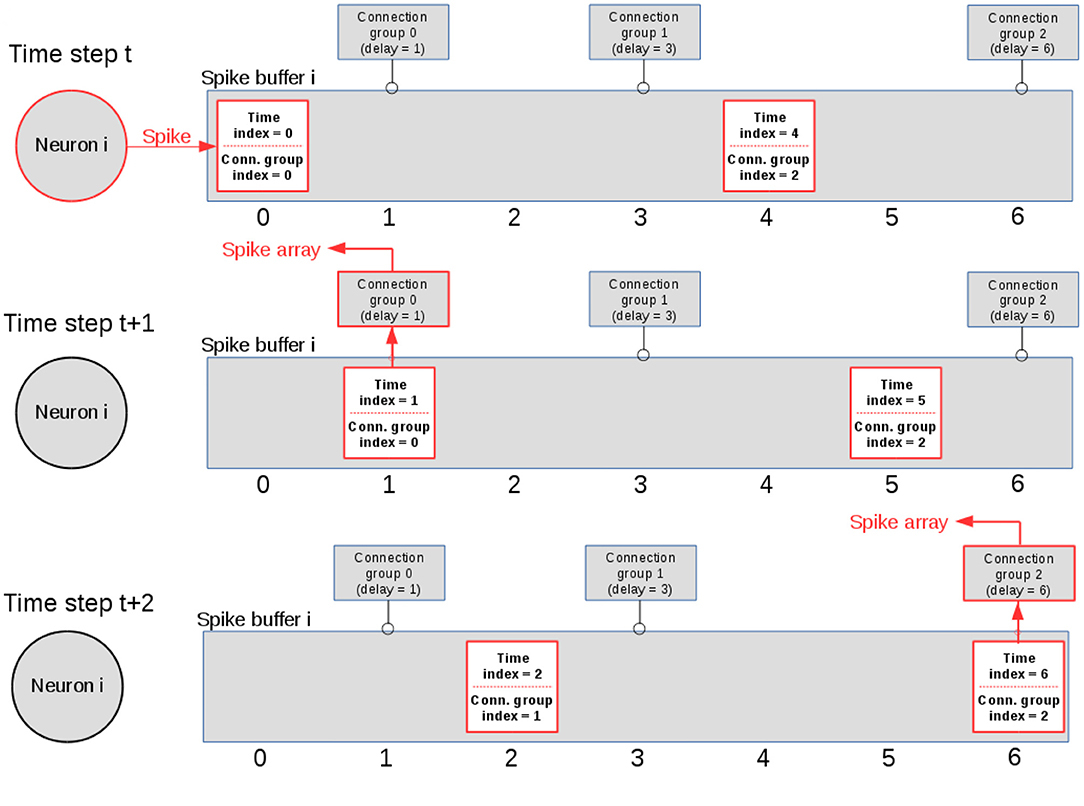
\includegraphics[width=\columnwidth]{figures/spike_buffer_array.jpg}
    \caption{Schematic representation of the spike buffer. At time step $t$ a neuron emits a spike, which starts with the time index and the connection group index equal to $0$. In the next time step, the spike increases $t_{\text{s}}$ by $1$ and, matching the delay of the connection group $0$, a spike event is sent to the spike array. This process is iterated until $i_{\text{g}}$ matches the last connection group and the spike event reaches it. Figure adapted from \cite{Golosio2021}.}
    \label{fig:spike_delivery_algorithm}
\end{figure}

Regarding multiple MPI process simulations, when a source node is connected to a target neuron belonging to a different MPI process, the spike buffer is created in the remote process, so that when the source node fires a spike, it is sent to the remote spike buffer at the end of the simulation time step through MPI communication.

\subsection{Network construction algorithm}
As mentioned in this section, NEST GPU has recently been equipped with a new algorithm for network construction that dynamically builds the network directly in the GPU \cite{Golosio2023}. 
Since the GPU memory capacity is one of the most important bottlenecks in GPU computing, an algorithm that handles such a task should be able to optimize the available memory as much as possible. In the creation of spiking neural network, a crucial role in this regard is held by the creation of the connections between network nodes. Indeed, in network models with natural density connectivity, the number of connections greatly exceeds the number of spiking devices: for instance, the multi-area model of \cite{Schuecker2017, Schmidt2018b, Schmidt2018} includes 4 million neurons and 24 billion synapses. We can thus understand the importance of having an efficient method for instantiating and organizing connections during network creation.\\
NEST GPU structures connections in the following way: each connection contains the source node index, the target node index, the receptor port index, synaptic weight and delay and the synaptic group index (which is non-zero only for plastic connections). Additional parameters can exist depending on the synapse model employed. Connections are stored in GPU memory using dynamically-allocated blocks with a fixed number of connections per block ($B$), which can be set by the user. It should not be too small to avoid having too many blocks and thus increase the execution time, and it should not be too big to avoid wasting memory leaving the last block not completely filled with connections. A reasonable value, that we usually use for large-scale simulations, can be $B=10^7$.\\
Every time a connection command is executed, if the last allocated block does not have enough free slots, one or more new blocks are created to store the remaining connections. 
After blocks have been allocated, connections are created by launching CUDA kernels (i.e., functions executed on GPU devices exploiting multiple CUDA-thread blocks) to set the connection parameters. In case some parameters have to be driven by a probability distribution, the cuRAND library\footnote{\url{https://developer.nvidia.com/curand}} is used to get the pseudo-random numbers given the distribution parameters. Figure \ref{fig:connection_creation} depicts an example of connection creation using this algorithm.

\begin{figure}[H]
    \centering
    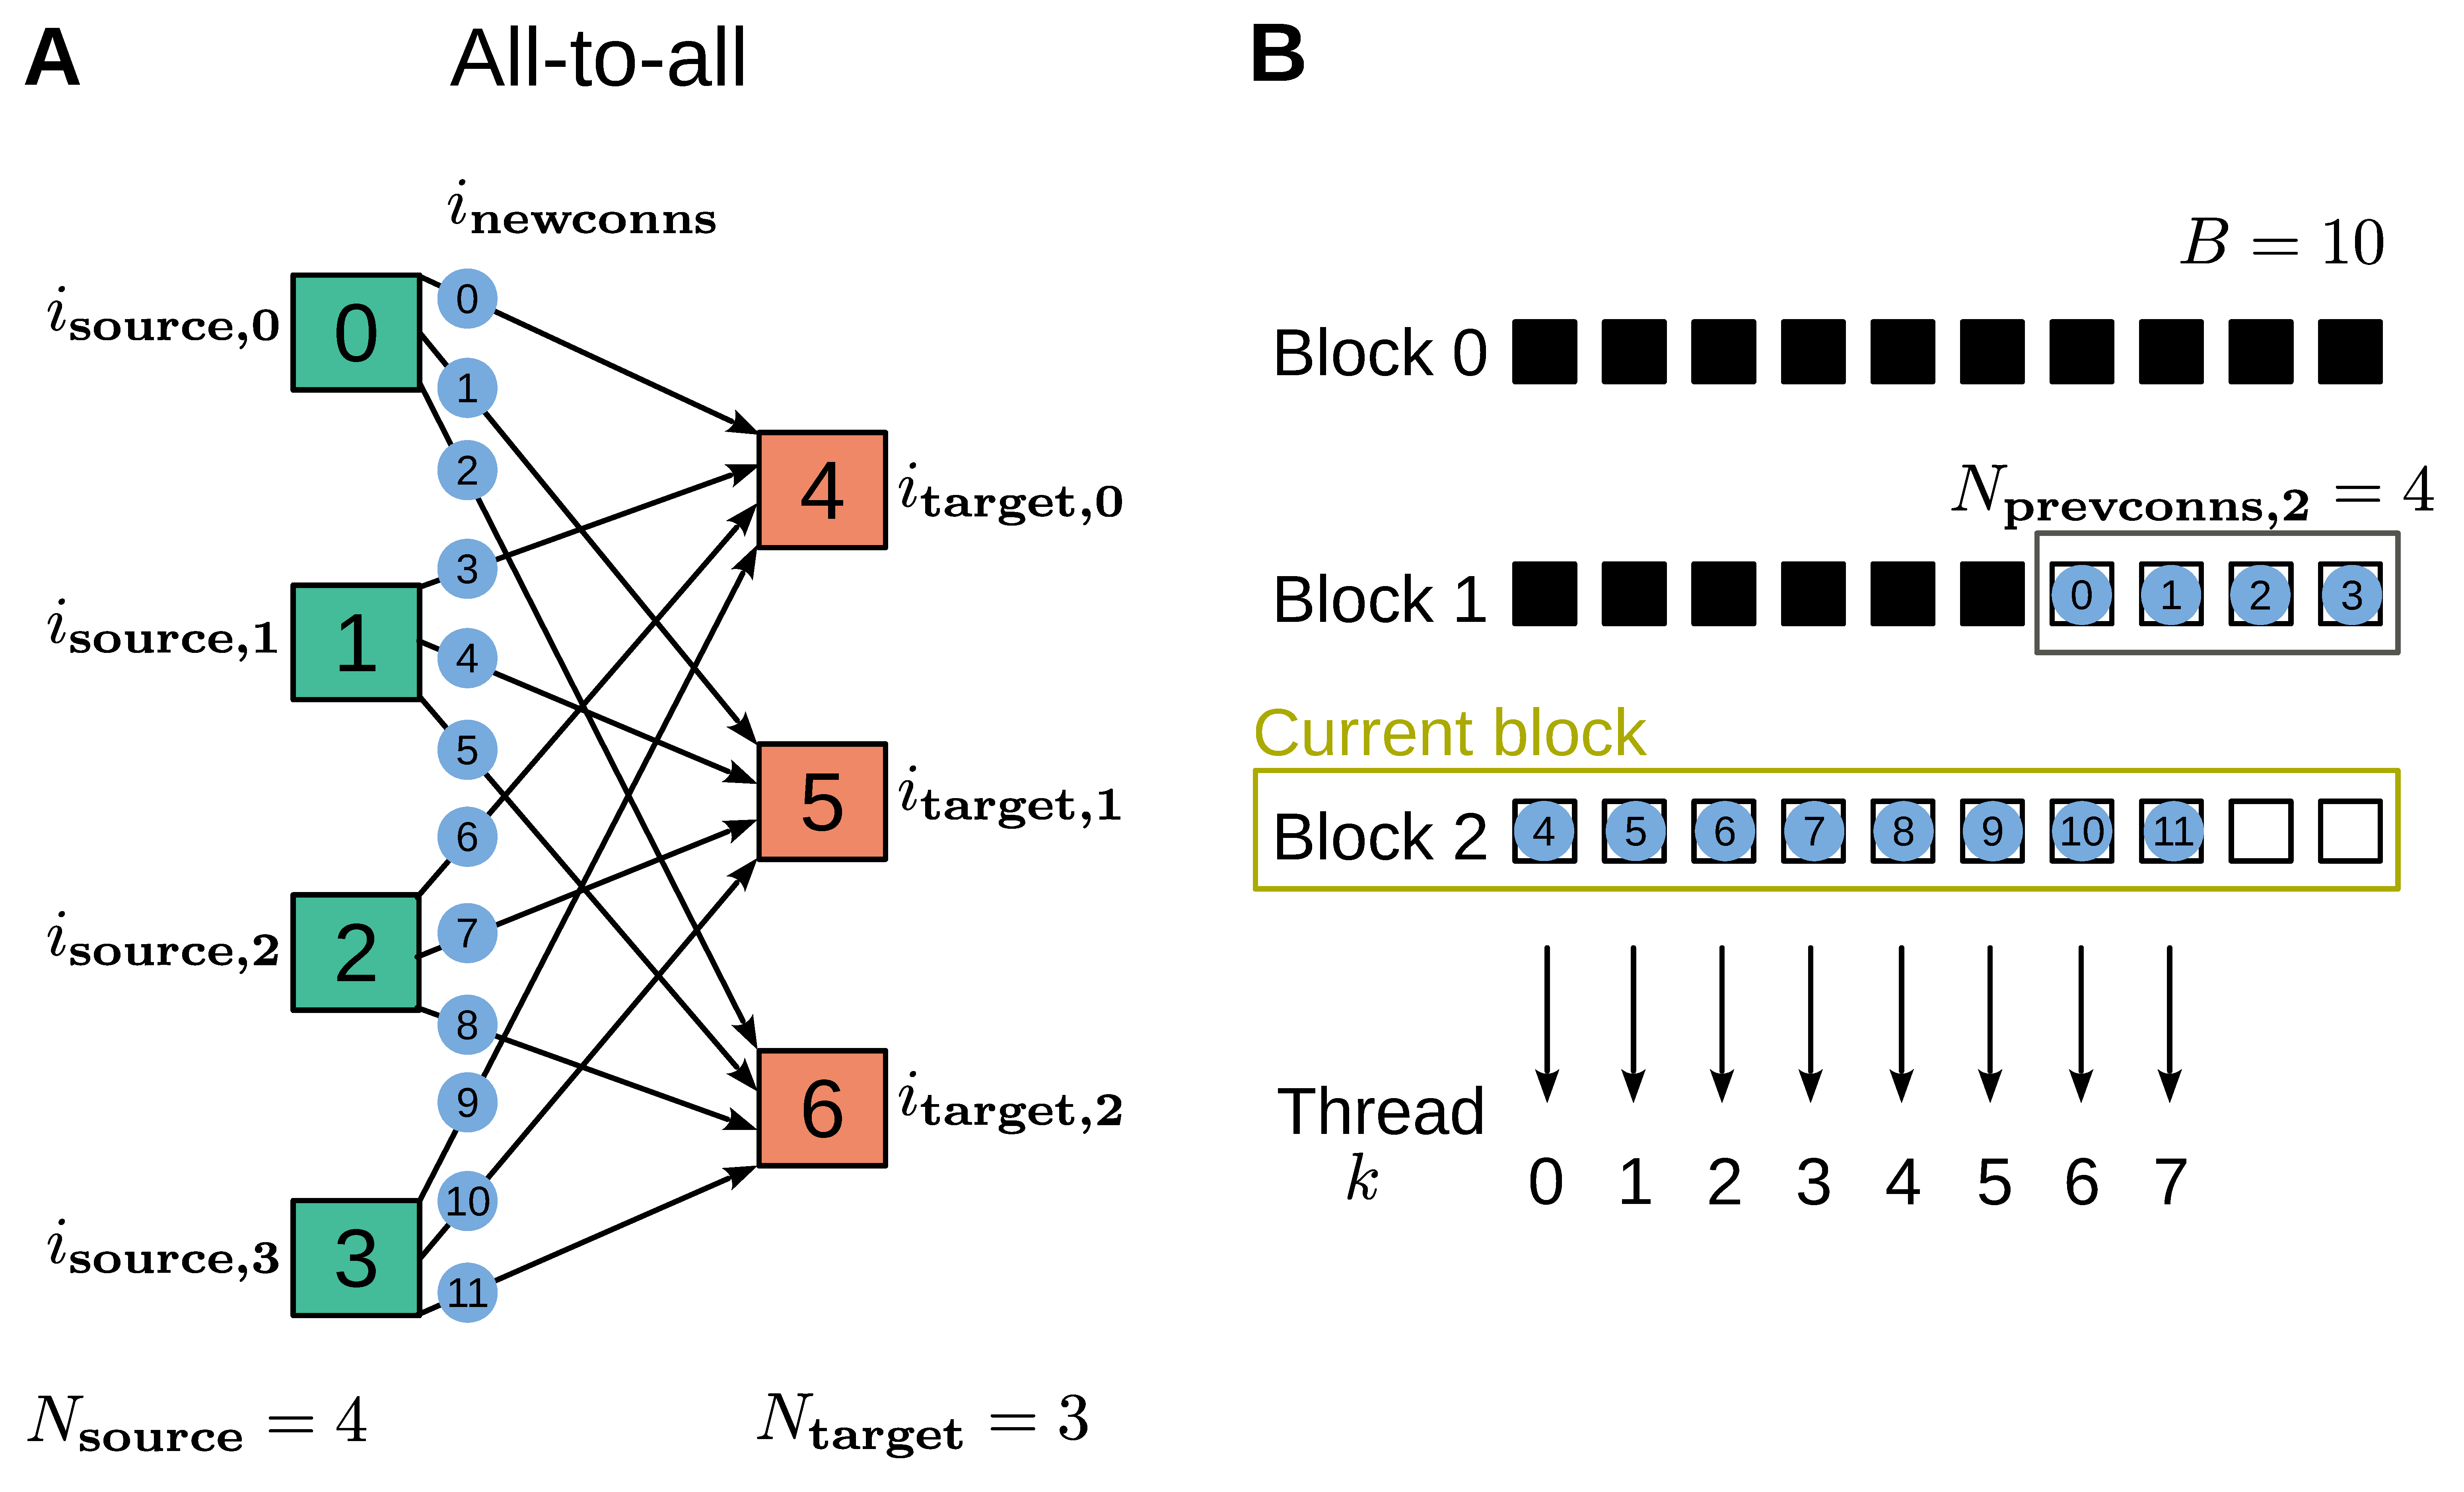
\includegraphics[width=0.85\columnwidth]{figures/conn_sketch.pdf}
    \caption{Example of connection creation. \textbf{(A)} All-to-all connection rule is used, so every source neuron (green) is connected with each target neuron (orange). Here, $12$ connections are created and the same amount of slots in the connection blocks have to be allocated.
    \textbf{(B)} Memory slots allocated in the blocks, that have already allocated memory for previous connections (full black squares). To store all the new connections, a new block is created. Finally, an appropriate number of CUDA-threads per block ($k$) is used to create the connections. Figure from \cite{Golosio2023}.}
    \label{fig:connection_creation}
\end{figure}

Once connections are created, they must be organized properly to optimize the spike transmission using the spike buffer. For this reason, connections are divided into groups, so that connections from the same group have same source node and same synaptic delay. Those groups are, indeed, the connection groups discussed in the previous section and depicted in Figure \ref{fig:spike_delivery_algorithm}. In order to organize connections in this way, connections have to be sorted using two sorting keys hierarchically, i.e., the index of the source node as first key and the delay as second key. Such a process is done after the dynamical creation of the connections, in a stage called \textit{calibration} phase. The sorting algorithm employed is an extension of radix-sort \cite{Cormen2009} applied to an array organized in blocks, based on the implementation available in the CUB library\footnote{\url{https://nvlabs.github.io/cub}}.\\
Once the connections are sorted, their groups must be adequately indexed, so that when a neuron emits a spike, the code has quick access to the groups of connections outgoing from this neuron and to their delays. This indexing is done in parallel using CUDA kernels on connection blocks with one CUDA thread for each connection. Finally, for each source node an array of size equal to the number of outgoing connection groups is constructed, and the arrays are then concatenated for all the source node into a single one-dimensional array. This avoids the creation of a large number of separate arrays, whose retrieval and usage would be more demanding than having a single one. This structure is used during spike delivery to properly index the spike event and send them to the proper connection groups.


\chapter{\textbf{Spiking network models and validation techniques}}
\label{chapter:models_and_validation}

\begin{tcolorbox}[colback=white,colframe=DarkRed,title=\textbf{Summary}]
Here we will introduce the spiking network models we used for benchmarking and validating the NEST GPU simulator.
After the description of the models, it will be described the statistical parameters used to evaluate their behavior, and how these parameters can be compared between simulators to ensure that different implementations of the same model provide a statistically compatible result.
\end{tcolorbox}

\section{Balanced network}
\label{sec:balanced_network}
The simplest network model used in this work is the so-called balanced network model. It is a sparsely connected network composed of an excitatory and an inhibitory population of integrate-and-fire neurons \cite{Brunel2000}. Under suitable conditions, this model can exhibit a stable average firing rate with asynchronous irregular spiking activity. External driving is granted by independent input spike trains targeting all neurons of both excitatory and inhibitory populations. In both NEST and NEST GPU this can be achieved through a single spiking device, called a \texttt{poisson\_generator}, which is able to send independent spike trains following a Poisson distribution through all its outgoing connections. In the considered model, a single Poisson generator is connected by excitatory connections to all neurons of both populations.\\
Neurons are connected through static synapses, which can be excitatory or inhibitory. Each neuron receives $\mathcal{C}_{\text{E}}$ connections from excitatory neurons and $\mathcal{C}_{\text{I}}=\mathcal{C}_{\text{E}}/4$ connections from inhibitory neurons using the \texttt{fixed\_indegree} connection rule, ergo each neuron is provided with $\mathcal{C}_{\text{E}}$ excitatory and $\mathcal{C}_{\text{I}}$ inhibitory input connections from other neurons of the model (see \cite{Senk2022} for a detailed description of the connection rule). Furthermore, the network is provided of $\mathcal{N}_{\text{E}}$ excitatory neurons and $\mathcal{N}_{\text{I}}=\mathcal{N}_{\text{E}}/4$ inhibitory neurons.

Figure \ref{fig:balanced_network} shows the structure of the network model following the graphical notation of \cite{Senk2022} for nodes and connections.
\begin{figure}[H]
    \centering
    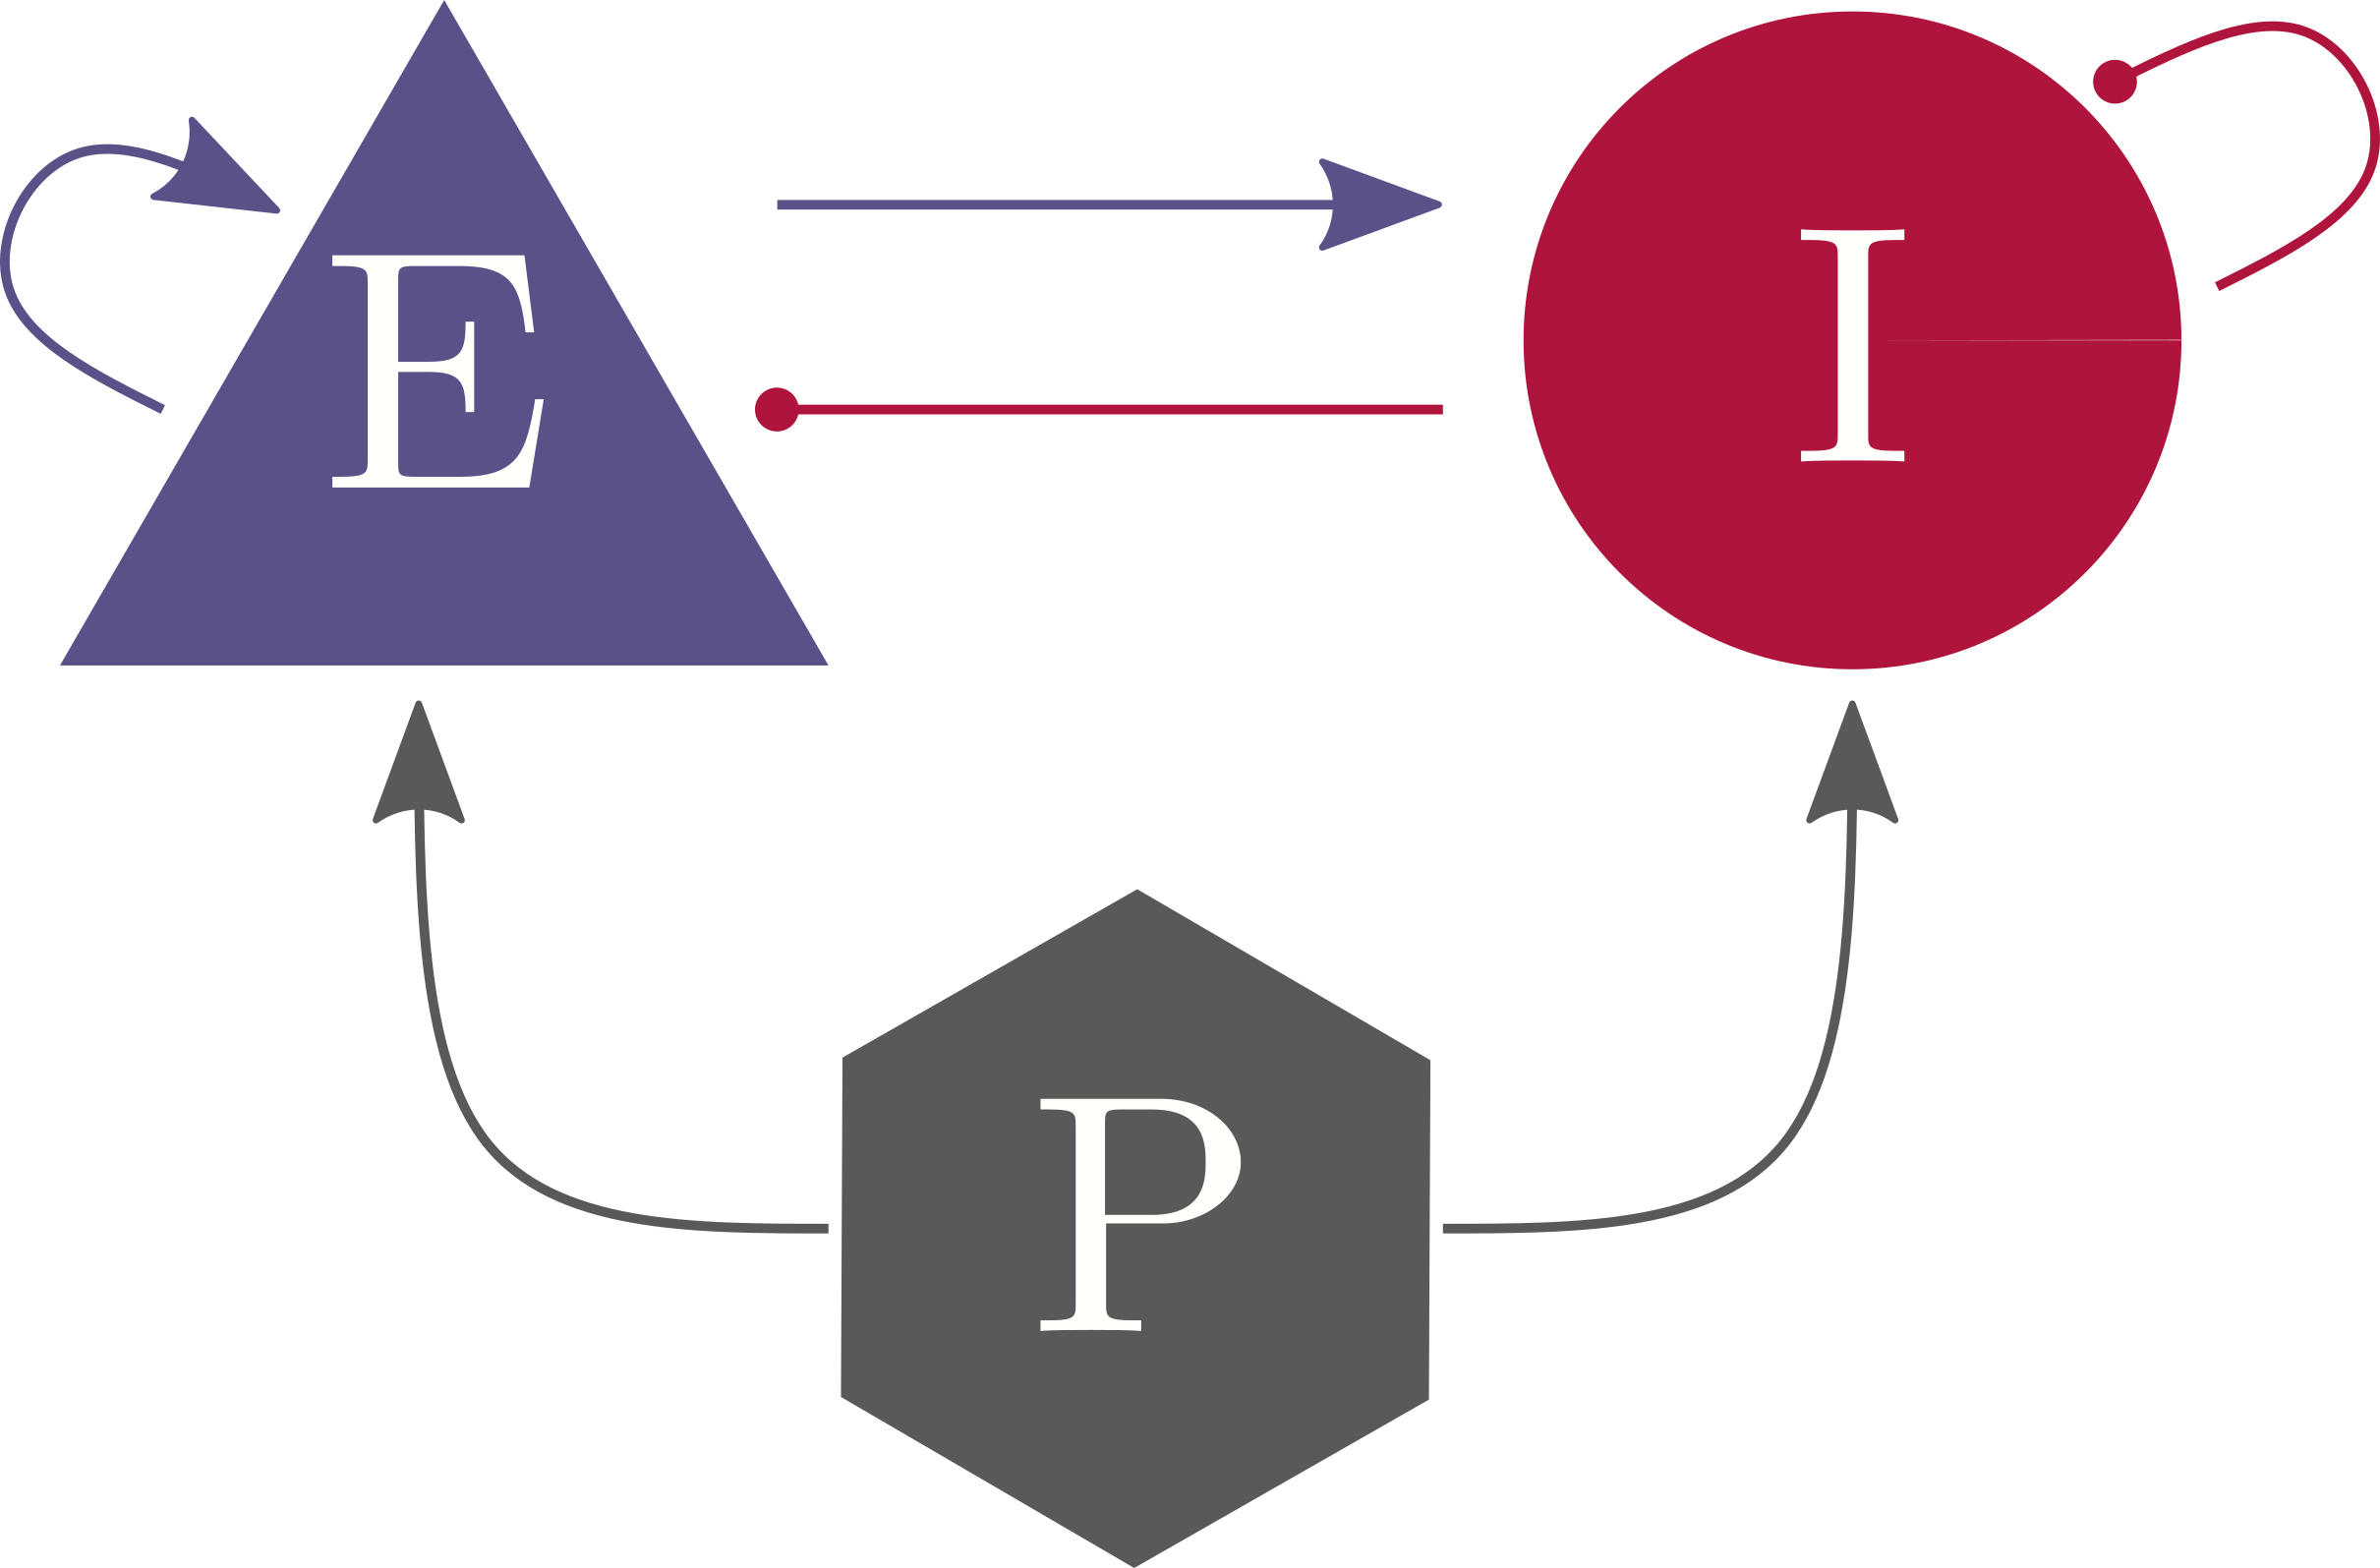
\includegraphics[scale=1.5]{figures/balanced_network.png}
    \caption{Schematic representation of a balanced network model. Here the graphical notation proposed in \cite{Senk2022} is used. Thus, the triangle, the circle and the hexagon represent, respectively, an excitatory, an inhibitory and stimulating device population (a Poisson signal generator in this case). Moreover, arrowhead connections are excitatory and circle-headed connections are inhibitory.}
    \label{fig:balanced_network}
\end{figure}

Such a network was also used in \cite{Golosio2021} in order to test the weak scaling performance of NeuronGPU, the prototype library of NEST GPU. Here, we propose a similar scaling using the most recent version of NEST GPU.\\
The neuron model implemented is the adaptive-exponential integrate-and-fire (AdEx) \cite{Brette2005} with conductance-based synapses and synaptic conductance modeled by an alpha function \cite{modeling_synapses}. An introduction of the neuron model can be found in Appendix \ref{app:balanced_network}, together with neuron and network model parameters.

\section{Cortical microcircuit}
\label{sec:cortical_microcircuit}
Originated from an integrated connectivity map, the cortical microcircuit model of \cite{Potjans2012} describes the neural circuit under $1$\,mm$^2$ of cortical surface. It is composed of around $77,000$ neurons and $3\cdot 10^8$ static connections and it is characterized by a layered structure that is based on the stratification of the cerebral cortex. Each layer (i.e., 2/3, 4, 5 or 6) has an excitatory (E) and an inhibitory (I) neuron population, for a total of eight populations: 2/3I, 2/3E, 4I, 4E, 5I, 5E, 6I, and 6E. All neurons are externally stimulated by a background input which can be originated from Poisson-distributed spike input or a DC input. The external input is needed to take into account  the signal coming from other regions of the cortex that are not included in the model. Moreover, neurons of layers 4 and 6 are additionally stimulated by a thalamo-cortical input designed as the previously described external input, in order to mimic the input coming from the thalamus. We can consider it as a multilaminar extension of the balanced network model described in Section \ref{sec:balanced_network}.\\
The neuron model employed is a leaky integrate-and-fire (LIF) with exponentially decaying postsynaptic currents. The differential equations underlying the neuron dynamics are integrated using the exact integration method of \cite{Rotter1999}. Synapses are static and the weight is chosen in order to have a defined average postsynaptic potential amplitude (see Chapter \ref{chapter:lif_adex_intro} for more details in this regard).\\
Such a model is able to show an asynchronous irregular spontaneous activity, compatible with the experimentally observed cell-type and layer-specific firing statistics. As we will see in the next section, it has been used as a building block for larger models \cite{Schmidt2018}, and has been used as a benchmark in several studies \cite{Knight2021, VanAlbada2018, Knight2018, Rhodes2019, Kurth2022, Heittmann2022}.\\
The model has been implemented in NeuronGPU (and thus in NEST GPU) in \cite{Golosio2021} and we evaluate the performance of the libraries on this model in \cite{Golosio2021, Golosio2023}.\\
Neuron and network model parameters are described in detail in Tables 1-4 of \cite{Dasbach2021} following the guidelines proposed in \cite{Nordlie2009}.

Figure \ref{fig:microcircuit} shows a scheme of the microcircuit model.
\begin{figure}[H]
    \centering
    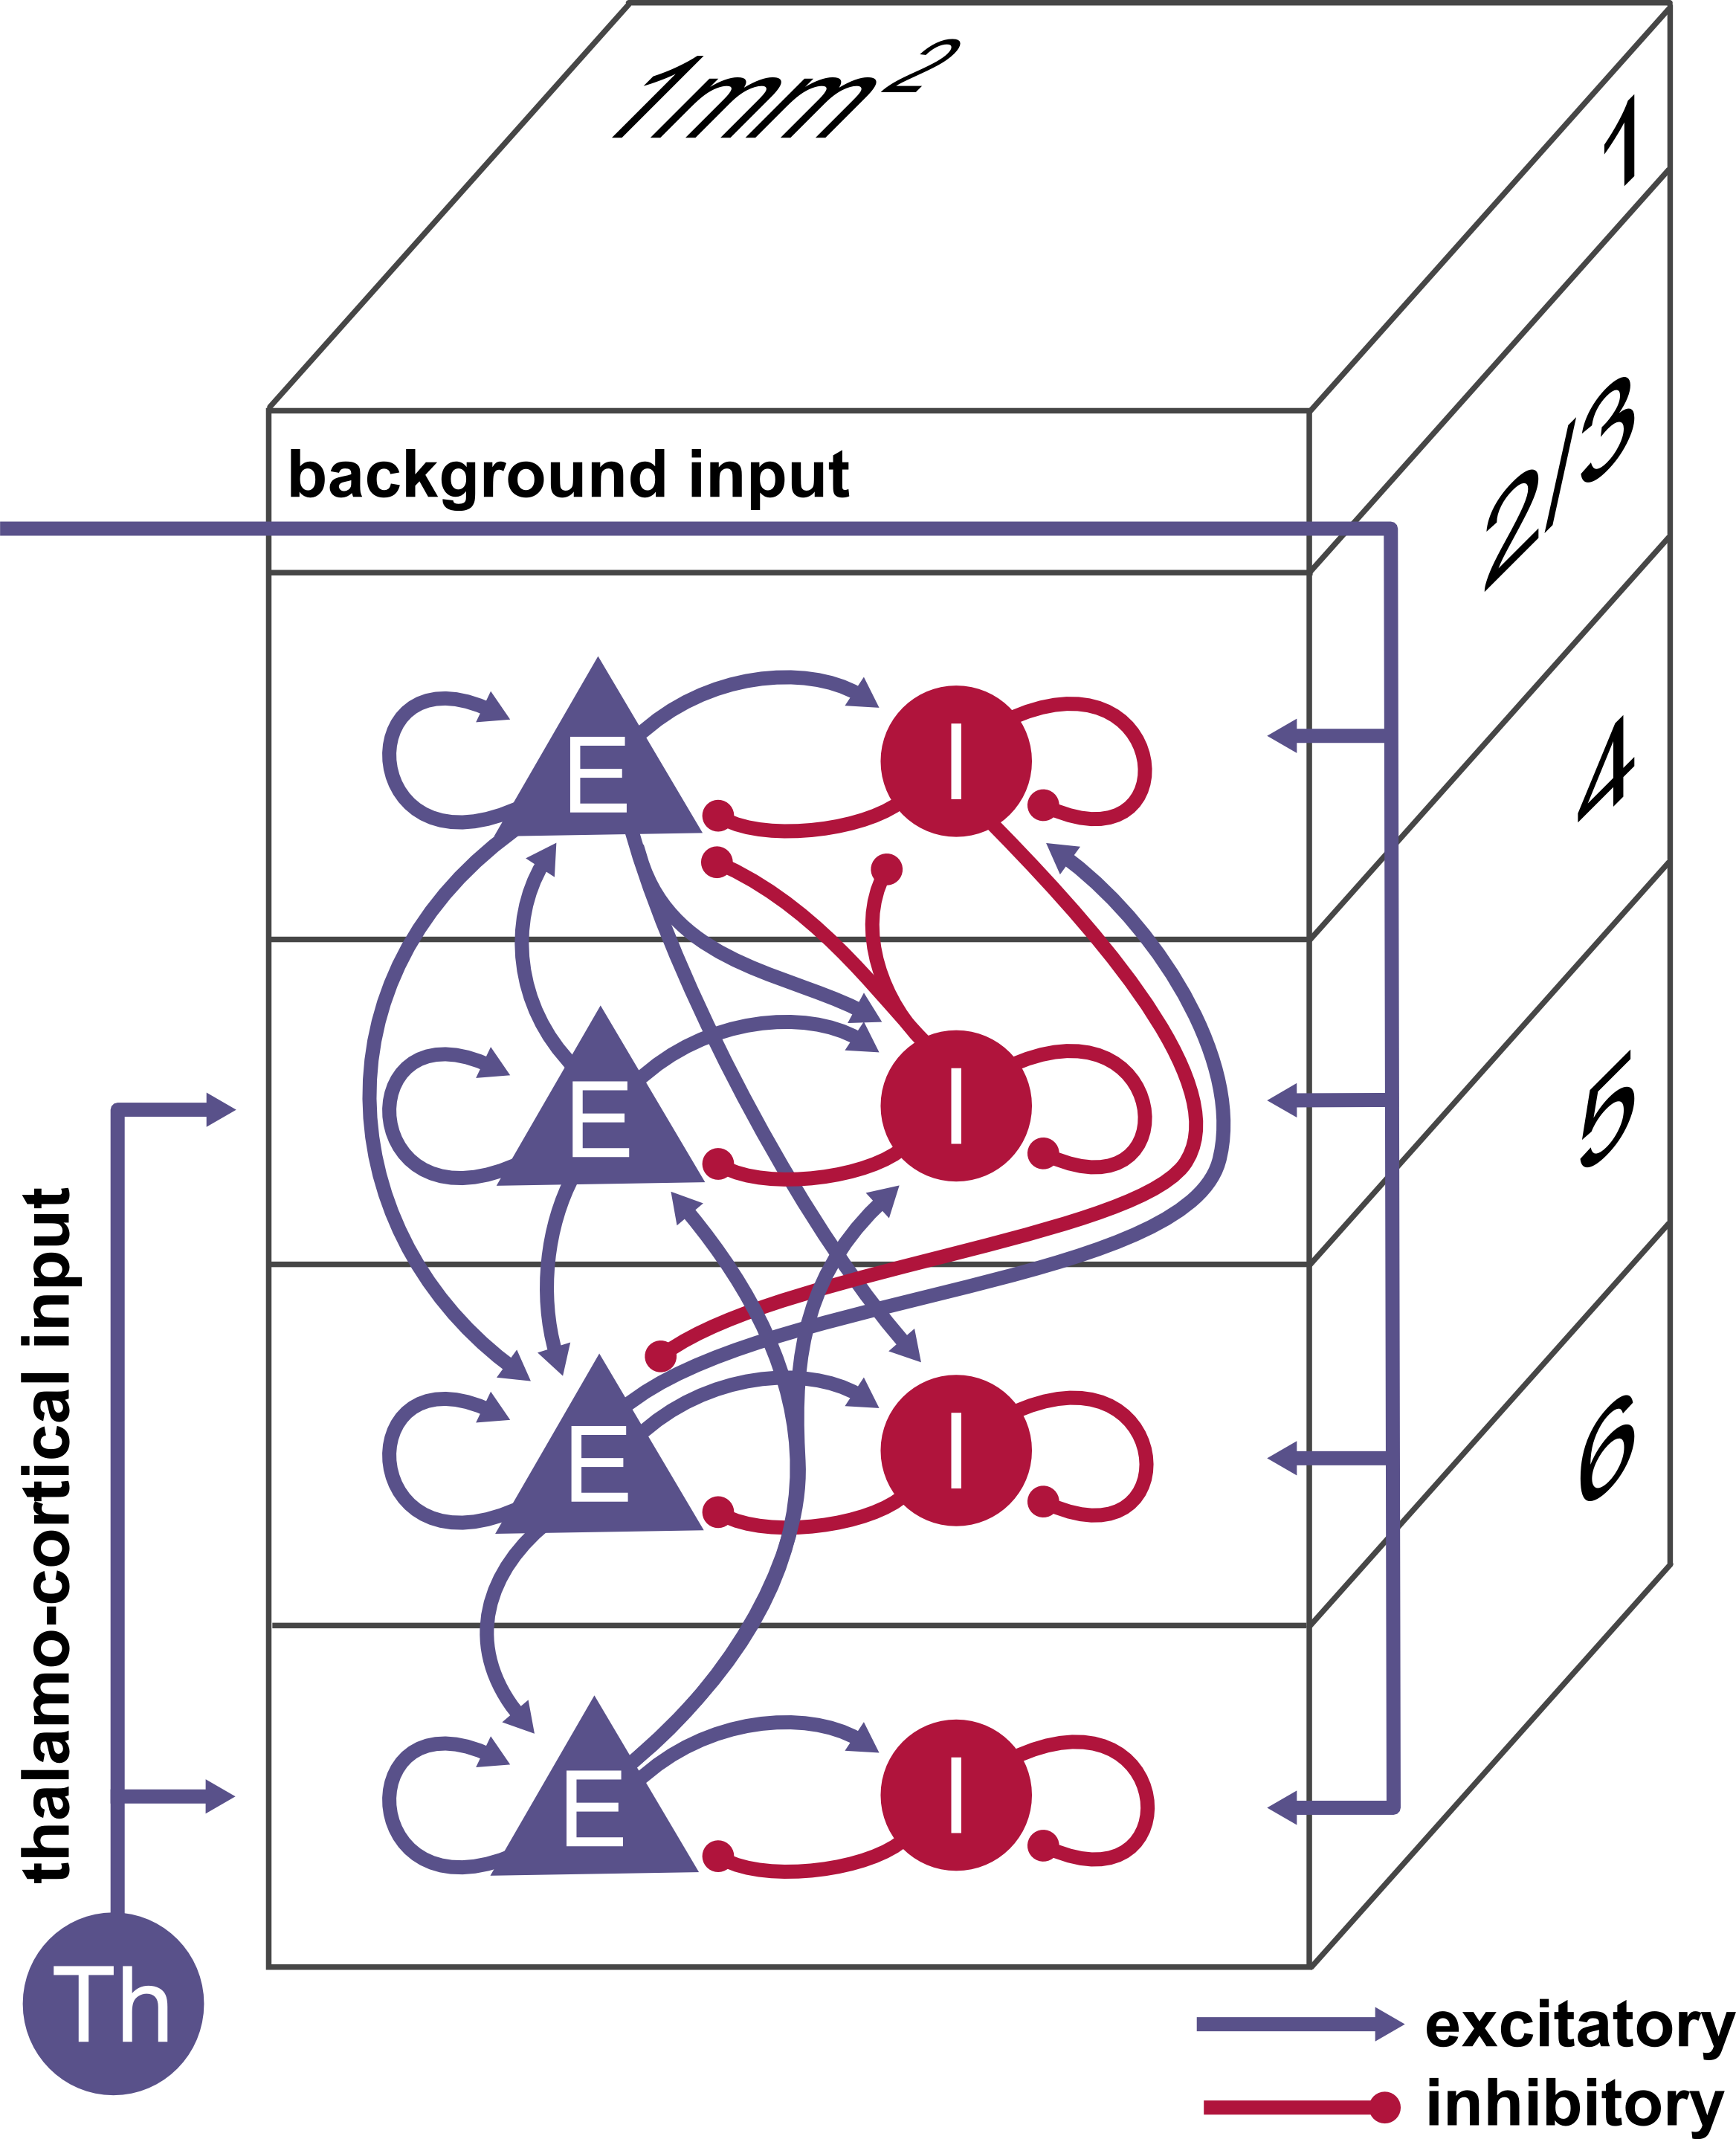
\includegraphics[scale=1.15]{figures/microcircuit.png}
    \caption{Scheme of the cortical microcircuit, from \cite{VanAlbada2018}. The scheme exhibits the layered structure of the network model, together with intra- and inter-layer connections. In particular, only connections with probability $>0.04$ are shown here.}
    \label{fig:microcircuit}
\end{figure}

\section{Multi-area model}
\label{sec:mam_description}
The multi-area model is a spiking network model able to describe the dynamics of the vision-related areas of one hemisphere of the macaque cortex \cite{Schmidt2018,Schmidt2018b}. In particular, the model is composed of 32 areas, each one described by a patch of $1$\,mm$^2$ size with full local density of neurons and synapses. This way, about 4 million neurons and 24 billions of synapses are simulated. Each area is designed similarly to the cortical microcircuit model of \cite{Potjans2012} described in the previous section. Thus, areas have a laminar structure with 4 layers, each one with an excitatory and an inhibitory population of neurons. Since one area (i.e., area TH) lacks of one layer, the total number of neuron populations in the network is 254. The local connectivity (i.e., within the same area) is a result of a scaling of the one of the cortical microcircuit of \cite{Potjans2012}. Also, the number of neurons for each microcircuit depends on experimental measurements done on every modelled area (e.g., neuron density and thickness of the cortical layer). The inter-area connectivity is based on database CoCoMac \cite{Bakker2012} of axonal tracing data, complemented with additional axonal tracing studies \cite{Markov2011,Markov2014} and statistical estimations reported in detail in \cite{Schuecker2017}.\\
The neuron model used is, as in the cortical microcircuit, the current-based LIF model with exponentially decaying postsynaptic potential. Moreover, the input coming from non-modeled regions of the brain is mimicked through Poisson spike trains, with frequency adapted for each neural population of the model.\\
Figure \ref{fig:mam} represents an overview of the multi-area model.
\begin{figure}[H]
    \centering
    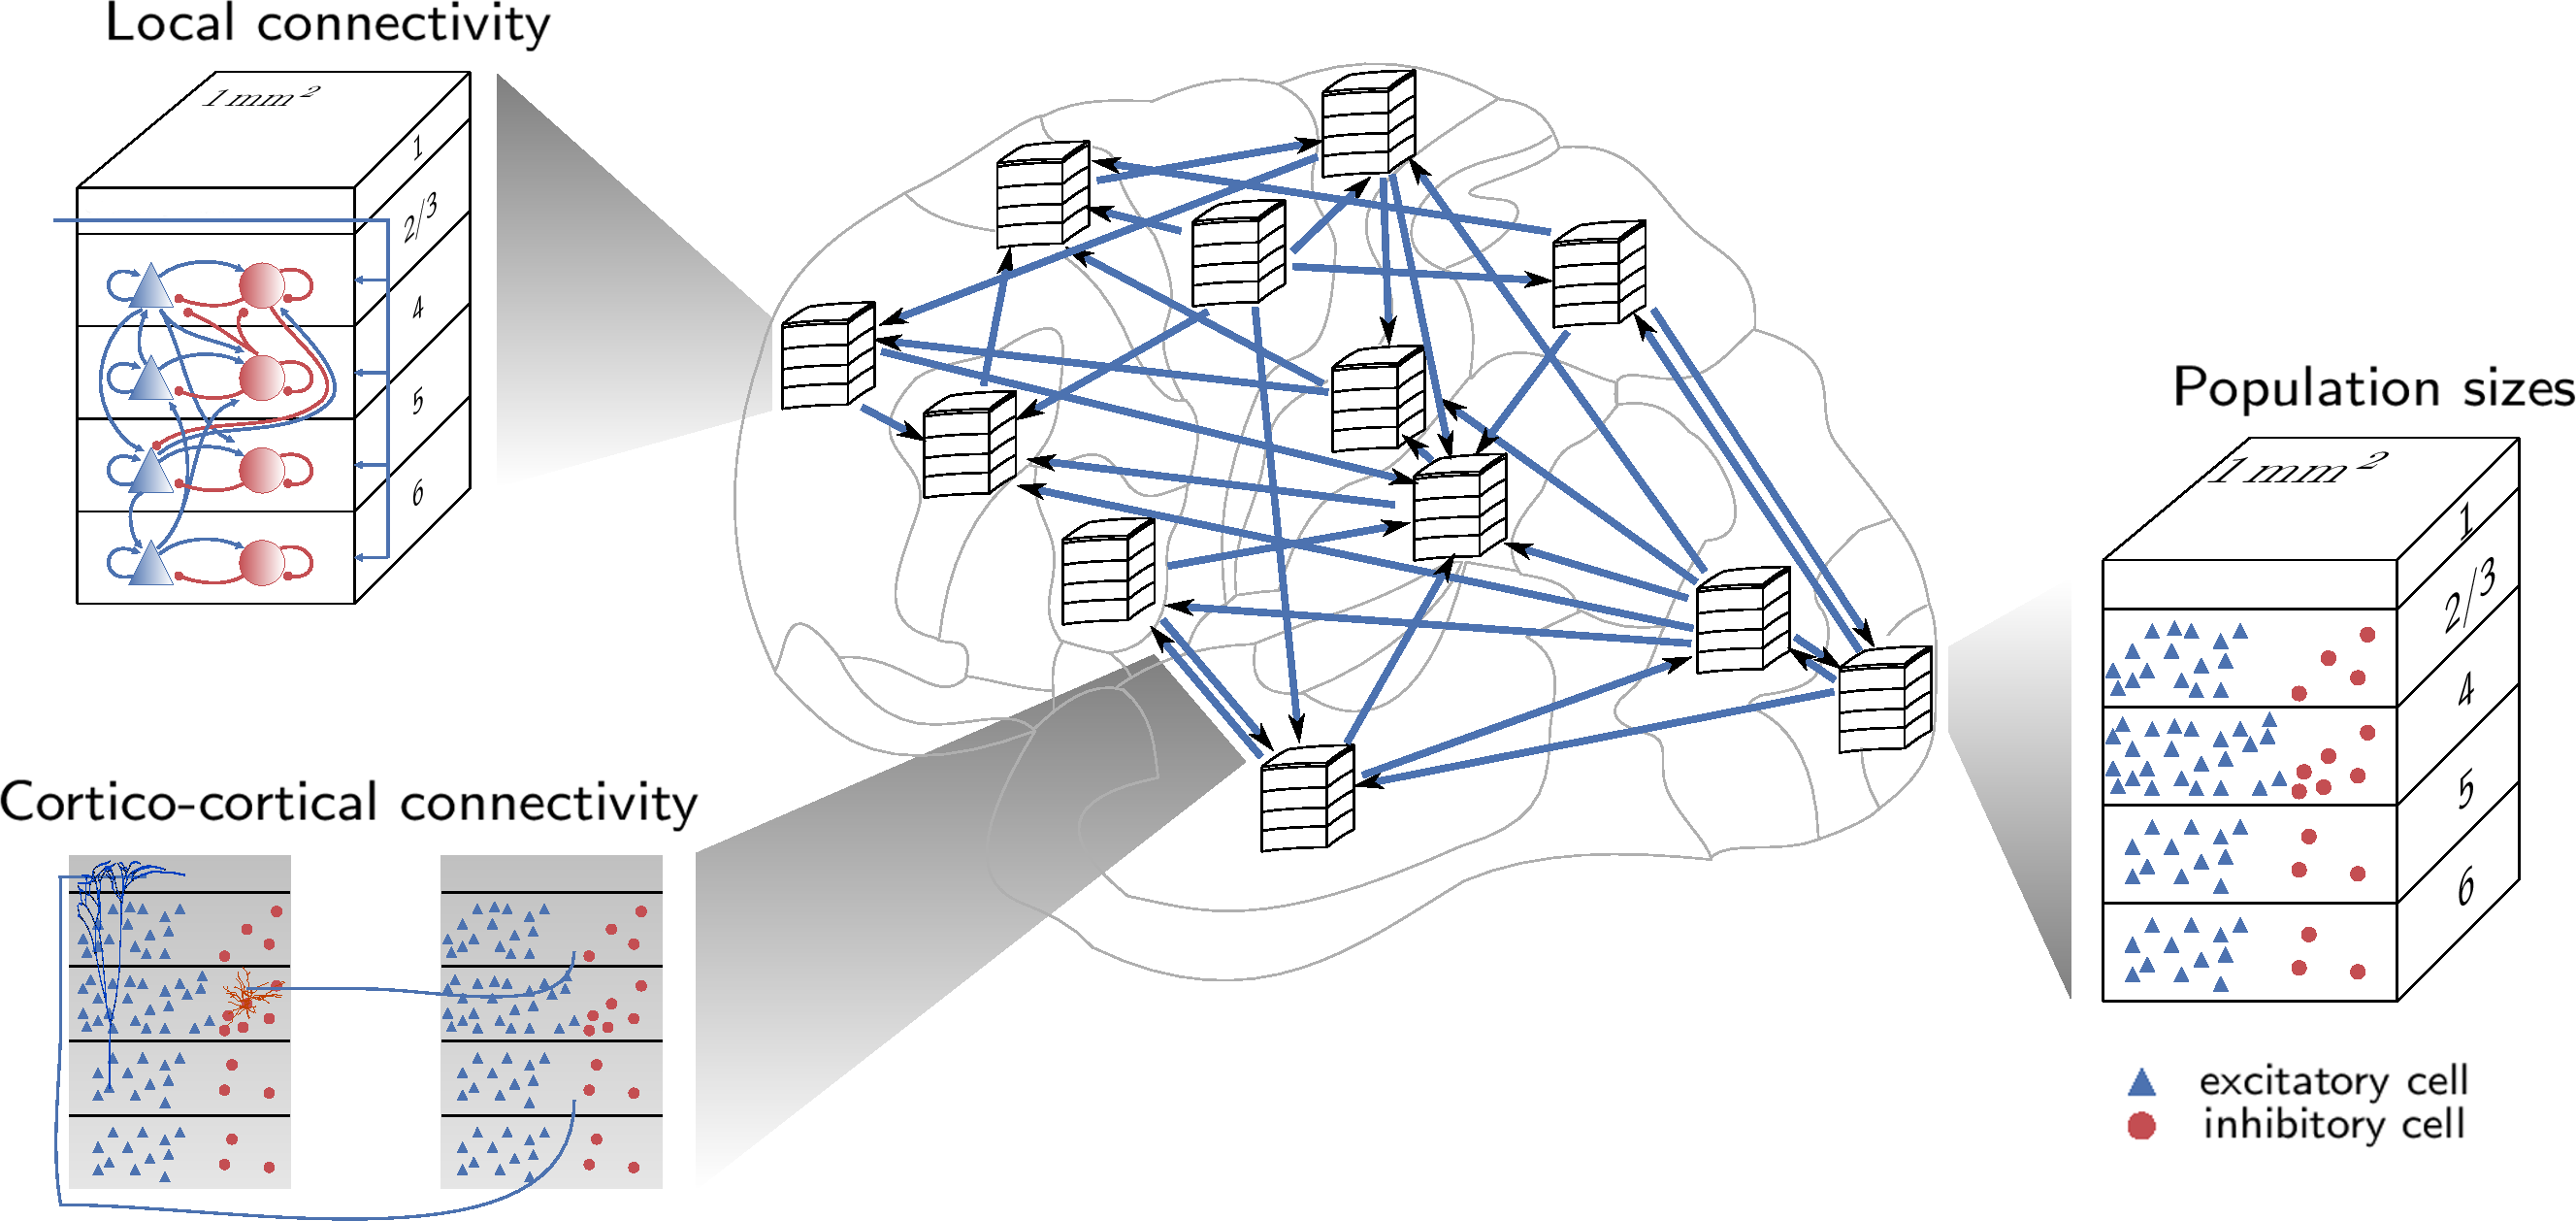
\includegraphics[width=\columnwidth]{figures/multiarea.png}
    \caption{Schematic representation of the multi-area model, adapted from \cite{Tiddia2022}.}
    \label{fig:mam}
\end{figure}

Such a model can show two activity states based on the synaptic strength of the cortico-cortical synapses with respect to the local synaptic weights. When the cortico-cortical synaptic strength is the same as the local one, the network reaches the so-called \textit{ground state}, in which the activity is asynchronous irregular without any relevant rate fluctuation. Indeed, such a state does not represent the resting-state recordings for spiking activity and functional connectivity. However, when cortico-cortical connections are increased, the network can reach the \textit{metastable state}, in which the network activity matches the recordings of resting-state activity of lightly anesthetized monkeys.
For further details on the multi-area model we refer to the original publications \cite{Schmidt2018, Schmidt2018b}.

\section{Validation techniques and benchmarking}
The described network models were implemented on NEST and the result of the simulations of these models were compared with experimental measurements (see for example \cite{Potjans2012,Schmidt2018}). Thus, NEST is a reliable and well established simulator we can use as a reference to ensure the correctness of the simulations of the same network models with NEST GPU. When implementing the same model on a different simulator, the first question that we need to answer is: \textit{did we build the right system?}
To answer such a question, after preliminary checks (e.g., verify that a single neuron responds in the same way when the same input is given), we have to establish a validation protocol able to assess whether the outcomes of the simulators are statistically compatible. To do so we need some quantitative estimations for each population, and a metric to compare these estimations obtained from the same population of the model in exam using different simulators.

\subsection{Getting the distributions}
\label{sec:KDE-EMD}
The simulation outcome that has been used to compare these models with experimental observations is the spiking activity. As proposed in several other works (such as \cite{VanAlbada2018, Knight2018, Dasbach2021, Heittmann2022}) we choose a set of statistical distributions related to the spiking activity of the neuron populations. In order to provide enough details on the statistical distributions we extracted from the data, we need to define what we actually measure from simulations and identify as spiking activity. Indeed, the outcome we get from the simulations is the spike train from each neuron of the population, identified with an ID. A spike train can be described by the equation
\begin{equation}
    \label{eq:spike_train}
    s_i(t)=\sum_k \delta (t-t_k^{(i)}) 
\end{equation}
where $\delta (\cdot)$ is a Dirac delta. Thus, a neuron spike train is just the collection of time values $t_j$ at which the neuron $i$ has emitted a spike. In addition, we need to describe another quantity functional for the estimation of the statistical distributions, which is the inter-spike interval (ISI). Given a spike train, the inter-spike interval (ISI) is defined as the time differences between two consecutive spikes. Thus
\begin{equation}
    ISI_i (t) = t_{k+1}^{(i)} - t_k^{(i)}
\end{equation}
Now that we have defined the spike train and the ISI, for each population we computed the following statistical distributions:
\begin{itemize}
    \item the average firing rate. For a single neuron it can be defined as
    \begin{equation}
        \nu_i (t) = \dfrac{1}{t}\int_{0}^{t} s_i(t) dt
    \end{equation}
    The distribution is then formed by the firing rates of the neurons belonging to the population calculated using the equation above. The average single neuron firing rate for a population is
    \begin{equation}
        \nu (t) = \dfrac{1}{N}\sum_{i=1}^{N} \nu_i (t)
    \end{equation}
    \item the coefficient of variation of the inter-spike intervals (i.e., CV ISI), thus the ratio between standard deviation and average of the inter-spike intervals
    \begin{equation}
    \label{eq:cvisi}
        CVISI_i = \dfrac{\sum_k (ISI_k^{(i)} - \langle ISI_k^{(i)} \rangle)^2}{\sum_k ISI_k^{(i)}}
    \end{equation}
    Like the firing rate, this is a quantity extracted from a single neuron, thus the population distribution is the collection of the $CVISI_i$ for all the neurons of the population;
    \item the pairwise Pearson correlation between spike trains, obtained by considering only a subset of 200 neurons for each population to have a reasonable compute time. To properly compute this statistical distribution, spike trains are binned using a time step of $2$\,ms (i.e., the neurons refractory time used when simulating the network models), so that at most one spike can occur at each bin. We call $b_i$ the binned spike train of the neuron $i$ and $\mu_i$ a vector with the same lenght of $b_i$ having all the entries equal to the average of the binned spike train. Then, Pearson correlation can be computed as follows
    \begin{equation}
    \label{eq:pearson_correlation}
        \mathcal{C}[i,j]=\dfrac{\langle b_i-\mu_i, b_j-\mu_j \rangle}{\sqrt{ \langle b_i-\mu_i, b_i-\mu_i \rangle \cdot \langle b_j-\mu_j, b_j-\mu_j \rangle}}
    \end{equation}
    where $\langle , \rangle$ represents a scalar product. Considering 200 neurons per population, the result of Equation \eqref{eq:pearson_correlation} is a $200\times 200$ matrix, and the distribution of the pairwise Pearson correlation is formed by the non-diagonal entries of the matrix.
\end{itemize}

The quantities we have just described are computed using the Elephant package \cite{elephant2018}. To form the raw distributions, it would be sufficient to apply a proper binning to the data and create the histograms. In this regard, distributions are binned following the Freedman-Diaconis rule, according to which the bin width is defined as
\begin{equation}
    \label{eq:fd_binning_rule}
    2\dfrac{\text{IQR}}{N^{1/3}}
\end{equation}
where $\text{IQR}$ is the interquartile range of the data and $N$ is the number of observations for each distribution. This way, we can obtain the raw distributions, which are indeed dependent from the random fluctuations of single simulations. In order to reduce such fluctuations, we applied a smoothing using the kernel density estimation (KDE) \cite{Rosenblatt1956, Parzen1962} with a Gaussian kernel. Having a set of values $x_i$ with $i=1,\dots, N$ and a bandwidth $h$, a Gaussian kernel $K(x,h)$ can be defined as
\begin{equation}
    K(x,h) = A \exp{\Bigl( -\frac{x^2}{2h^2} \Bigr)}
\end{equation}
where $A$ is a constant needed for normalization. The KDE for a point $y$ is then
\begin{equation}
\label{eq:kde}
    \rho_{K}(y) = \sum_{i=1}^{N} K(y-x_i, h)
\end{equation}
Hence, if $x_i$ are the set of values extracted from the spike data, each value can now be considered as a Gaussian function with a fixed width and properly normalized. The sum of the Gaussian functions obtained for each value produces the smoothed distribution.\\
To get the distributions, we still have to define the values for the normalization factor $A$ and the bandwidth $h$.
Regarding the normalization, each Gaussian function returned by Equation \eqref{eq:kde} is normalized to $1/N$, so that the final distribution is normalized to unity. Moreover, the bandwidth is optimized through the Silverman method \cite{Silverman1986}, so that
\begin{equation}
    h = 0.9\text{ min}\Bigl( \hat{\sigma}, \frac{\text{IQR}}{1.349} \Bigr)N^{-1/5}
\end{equation}
with $\hat{\sigma}$ standard deviation of the values and IQR the interquartile range. In the framework developed for this thesis, KDE is obtained using the function \\\texttt{sklearn.neighbors.KernelDensity} of the \texttt{scikit-learn} Python library \cite{scikit-learn}.
For more clarity, the next figure depicts a simple application of KDE.
\begin{figure}[H]
    \centering
    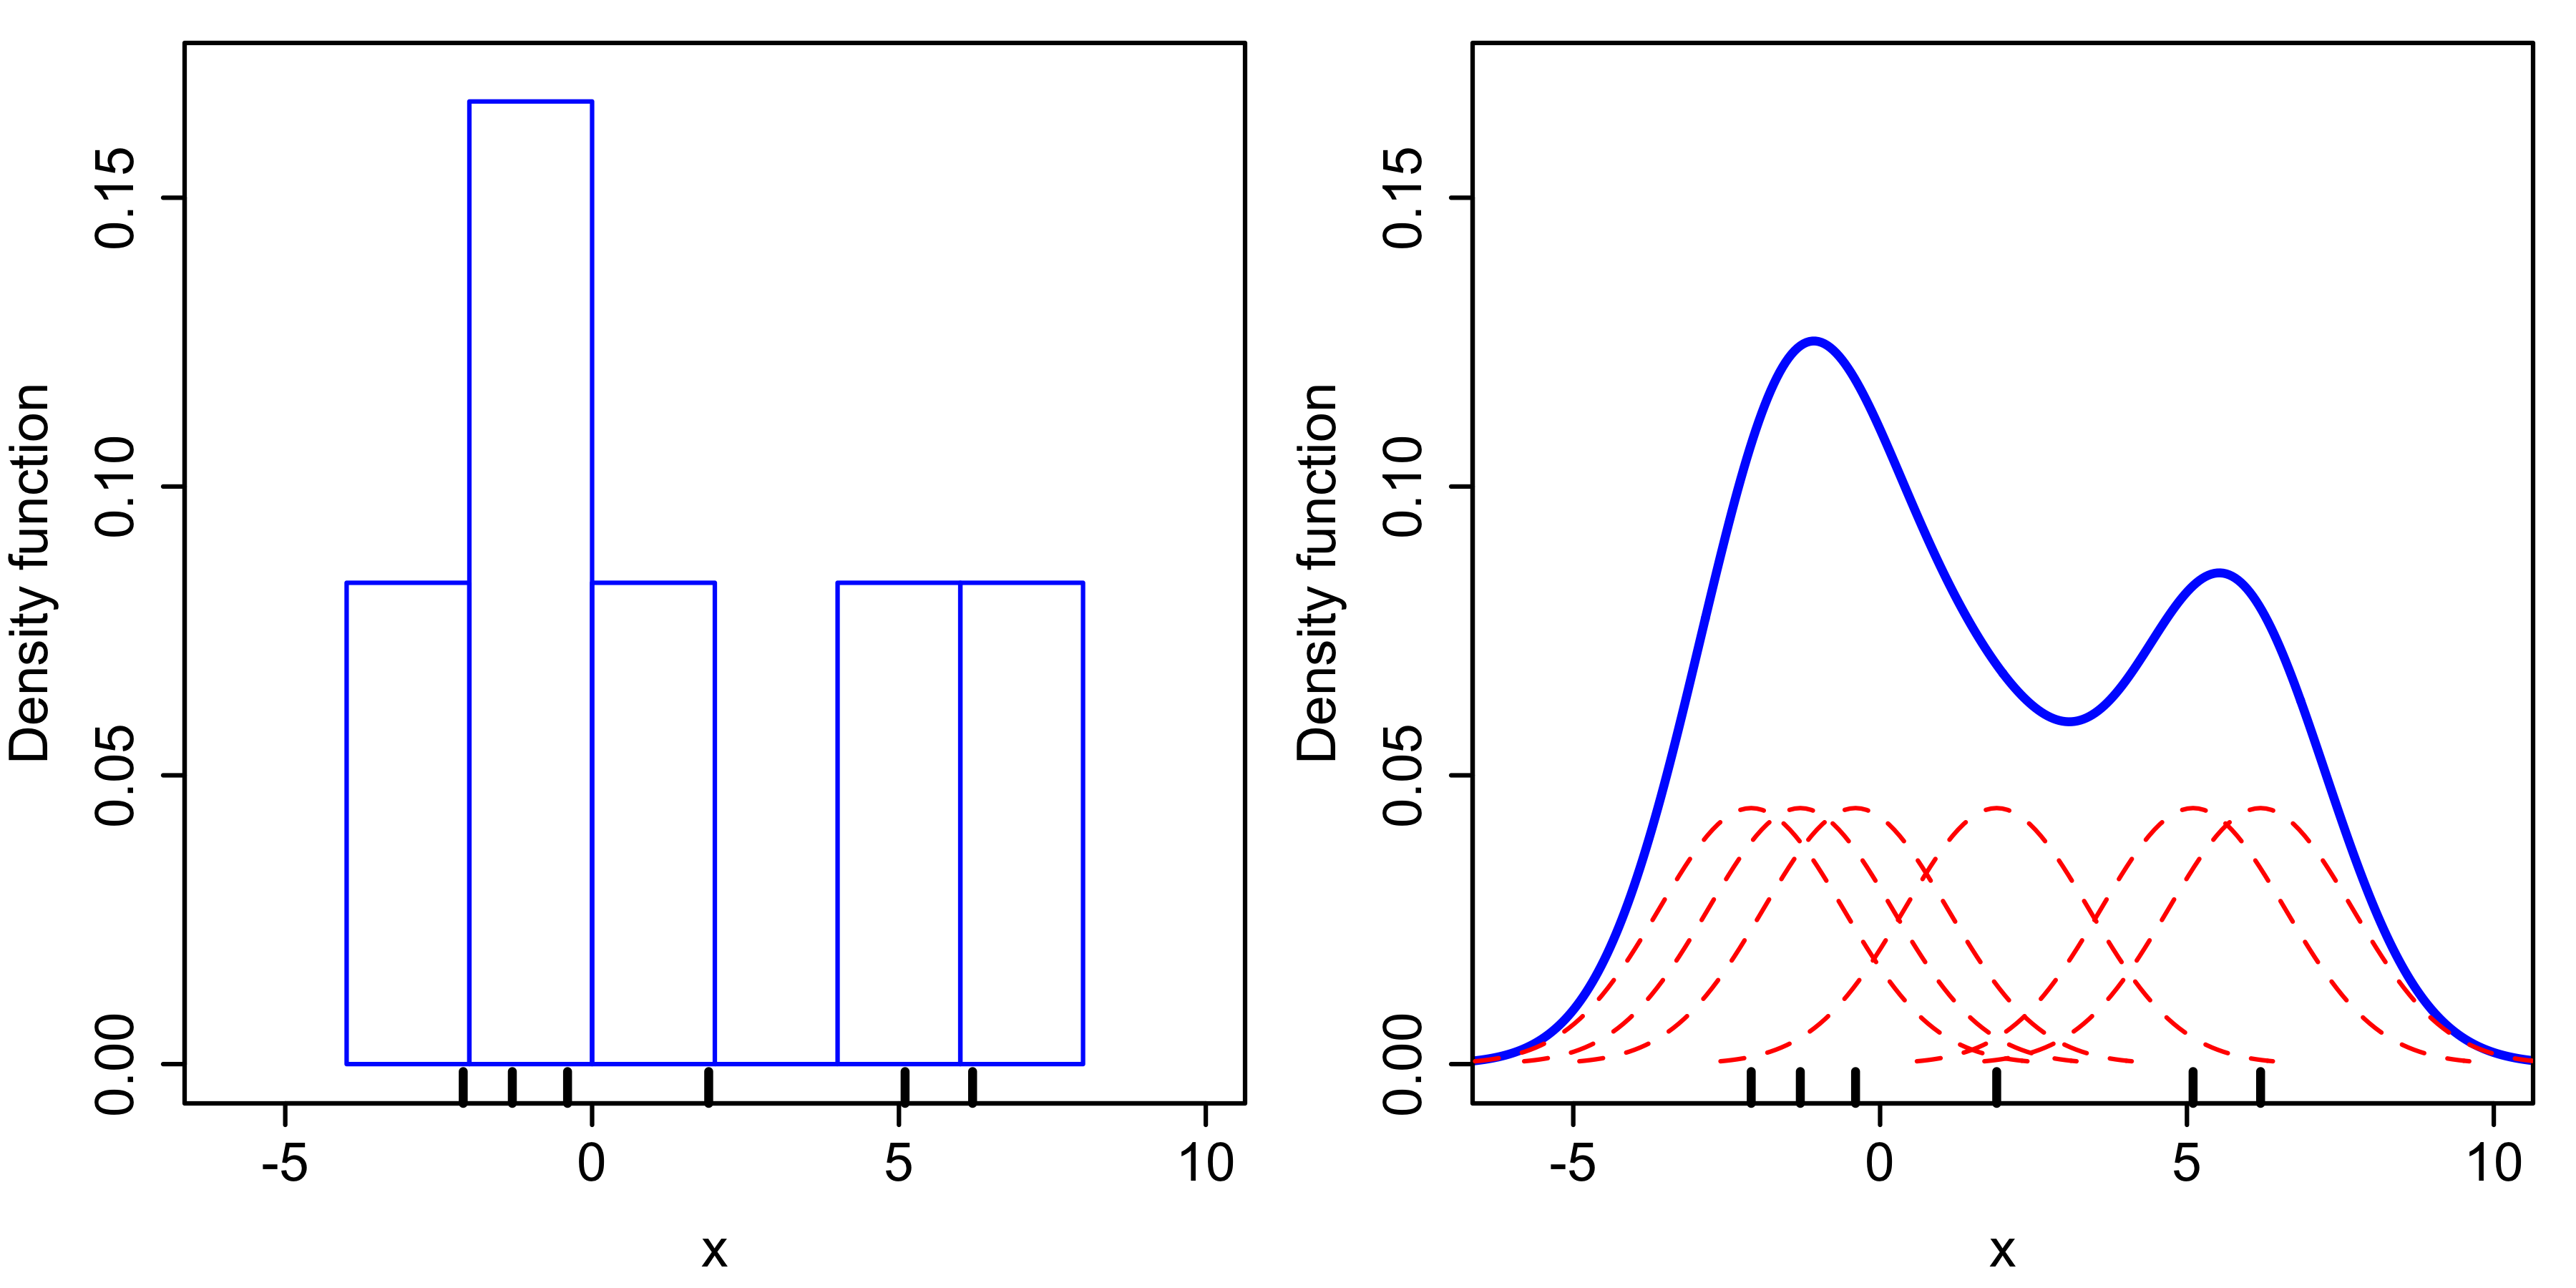
\includegraphics[width=0.8\columnwidth]{figures/KDE_example.png}
    \caption{Example of application of KDE to a simple data set. Left panel shows the histogram obtained from the data shown below as vertical black dashes. On the right, KDE is applied to data. Red-dotted lines represent the Gaussian kernels from each value that belongs to the data set, whereas the blue line is the KDE, defined as the sum of the single Gaussian kernels. Figure from \cite{kde_wiki}.}
    \label{fig:kde}
\end{figure}

This way we are able to obtain a continuous function able to reduce the small variability observed by single simulations that used different seed for random number generation. Indeed, the seed plays a crucial role in our validation framework, and the next subsection describes its role in detail.

\subsection{Getting the metric to compare the distributions}
\label{sed:validation_protocol}
The validation protocol adopted to statistically compare the results of the spiking activity obtained from different simulation codes (i.e., NEST and NEST GPU) is described below:
\begin{enumerate}
    \item we perform a set of simulations (e.g., $10$) using NEST, and we do the same with NEST GPU. Each simulation should use a different seed for random number generation;
    \item we perform an additional set of simulations of NEST (i.e., the simulator taken as a reference) using a different set of seeds, in order to estimate the variability of NEST when using different seeds;
    \item we compute, using a proper metric, the pairwise comparison between the distributions obtained by the two different simulators (e.g., the first simulation of NEST compares the distributions with the first simulation of NEST GPU, etc). This way we collect a set of values that quantifies the difference between the two simulators for each distribution, which we can call \textit{NEST-NEST GPU};
    \item we can do the same but comparing the two sets of simulations using NEST, obtaining the \textit{NEST-NEST} dissimilarity measure (or distance);
    \item we plot side by side the \textit{NEST-NEST GPU} and \textit{NEST-NEST} values to evaluate the differences that arise because of the different simulator employed and the one that can arise because of a different seed for random number generation when using the same simulator.
\end{enumerate}

With this approach we have a more quantitative method for the validation of the NEST GPU simulator with respect to a simple comparison of the distributions that can be done by simply showing the distributions in the same plot.\\
Now a questions remains to be answered: \textit{which metric, or dissimilarity measure, should we choose?}
For example, in \cite{Golosio2021} for the comparison of NEST and NeuronGPU in the simulation of the cortical microcircuit model, we used the Kullback-Leibler divergence ($D_{KL}$) \cite{Kullback1951}, which is defined as
\begin{equation}
    D_{KL} (p,q) = - \sum_i p_i\log\Bigl( \dfrac{p_i}{q_i} \Bigr)
\end{equation}
where $p$ and $q$ are two probability distributions with the index $i$ running on the sampling points of the distributions. The divergence measures the degree of dissimilarity of $p$ with respect to a reference distribution $q$. However, in \cite{Tiddia2022} we moved to the Earth Mover's Distance (EMD) because of its metric properties that make it symmetric and more specific in detecting the degrees of dissimilarity among the distributions. EMD computes the distance between two probability distribution and its name resembles a problem of soil reshaping. Indeed, the two distributions can be intended as two piles of soil, with one of them that has to be arranged in order to have the same shape as the other one. In this case, EMD represents the minimum amount of work needed to move the soil from one pile in order to have the desired distribution of soil. Returning to our distributions, EMD measure the work that has to be done to reshape a distribution in order to be like the target one. From a mathematical point of view, EMD is equivalent to the $1^{\mathrm{st}}$ Wasserstein distance between two distributions.\\
The Wasserstein distance is defined as follows \cite{Panaretos_Zemel, Frohmader_Volkmer}: let $\chi$ be a metric space endowed with a metric $d$ and $\mu$ and $\nu$ be two probability measures on $\chi$. Also let $\Gamma (\mu, \nu)$ be the set of probability measures $\gamma$ on $\chi \times \chi$ so that the measure $\gamma$ has marginals $\mu$ and $\nu$ on each axis. The $p^{\mathrm{th}}$-Wasserstein distance can be written as
\begin{equation}
    \label{eq:p-Wasserstein}
    W_p (\mu, \nu)=\Bigl( \inf_{\gamma \in \Gamma (\mu, \nu)} \int_{\chi \times \chi} d(x,y)^p d\gamma (x,y) \Bigr)^{1/p}
\end{equation}
This relation yields the given interpretation of the Earth Mover's Distance. In particular, given a $\gamma \in \Gamma (\mu , \nu)$ and two locations $(x,y)$, the quantity $d(x,y)^p$ quantifies the amount of work necessary to move a unit of mass from $x$ to $y$, and the infimum of the integral thus returns the minimum amount of work needed to reshape $\mu$ distribution into $\nu$.

Furthermore, equation \eqref{eq:p-Wasserstein} can be rewritten when $\chi = \mathbb{R}^1$ (ergo $d(x,y)=|x-y|$). Letting $F_{X}$ be the cumulative distribution function (CDF) of a distribution $X$ and $F^{-1}_{X}(q) = \inf \{x : F_{X}(x)\geq q\}, q \in (0,1)$ the quantile distribution of $X$ (i.e. the inverse cumulative distribution), it is shown in \cite{Ramdas_Trillos_Cuturi} that
\begin{equation}
    \label{eq:p-Wasserstein_icdf}
    W_p (\mu, \nu) = \Bigl( \int_{0}^{1}|F^{-1}_{\mu}(\alpha) - F^{-1}_{\nu}(\alpha)|^p d\alpha \Bigr)^{1/p}.
\end{equation}
In the particular case of the $1^{\mathrm{st}}$ Wasserstein distance (i.e. $p=1$), as discussed in \cite{Vallender}, equation \eqref{eq:p-Wasserstein_icdf} reduces to
\begin{equation}
    \label{eq:EMD}
    W_1 (\mu, \nu) = \mathrm{EMD}(\mu, \nu) = \int_{\mathbb{R}}|F_{\mu}(t) - F_{\nu}(t)| dt.
\end{equation}
that is the equation used by the Python scientific library SciPy \cite{SciPy} to compute this metric with the \texttt{scipy.stats.wasserstein\_distance} function, which takes the values of the distributions as input, computes their CDF and finally returns the result of the integral \eqref{eq:EMD}.\\
In conclusion, the validation process enables to show side by side the distributions of the EMD values obtained from the comparisons \textit{NEST-NEST GPU} and \textit{NEST-NEST}. The next chapter describes the validation work we performed using NEST GPU for the simulation of the cortical microcircuit model and the multi-area model. Then, we analyze the performance of NEST GPU in the simulation of these models and the scaling performance of the simulator through simulations of the balanced network model.

%%%%%%%%%%%%%%%%%%%%%%%%%%%%%%%%%%%%%%%%%%%%%%%%%%%%%%
\chapter{\textbf{NEST GPU validation}}
\label{chapter:comparison_NEST_NGPU}

\begin{tcolorbox}[colback=white,colframe=DarkRed,title=\textbf{Summary}]
Here NEST and NEST GPU are compared in terms of neural activity of single neurons and the models discussed in the previous chapter with the aim of providing a solid validation workflow to be easily employed when validating NEST GPU. In particular, NEST GPU is validated on the simulation of the cortical microcircuit model and the multi-area model previously introduced.
\end{tcolorbox}

\section{Single neuron simulation}
A first control that we usually do when checking the compatibility of NEST GPU is a simple simulation of single neuron models targeted by few spikes or injected with a constant current, to be compared with an analogous NEST simulation. Indeed, one of the tests NEST GPU performs after installation regards the response of such a stimuli by the membrane potential of the several neuron models implemented in the simulator. For instance, Figure \ref{fig:single_neurons_membrane_potential} shows the membrane potential of two different neuron models injected with two spikes delivered using connections with different delays. In panel A is depicted the response of a LIF neuron with exponential current-based synapses (\texttt{iaf\_psc\_exp} in NEST and NEST GPU), whereas in panel B is shown the response of an AdEx neuron with conductance-based synapses and synaptic conductance modeled as an alpha function (\texttt{aeif\_cond\_alpha} in NEST and NEST GPU).\\
The same simulation is also performed in NEST, and the results are here compared.
In particular, the first signal the neuron receives is excitatory (i.e., is transmitted through a connection with positive weight), whereas the following one elicit a drop in the membrane potential (ergo the synapse is inhibitory, and thus with a negative synaptic weight).\\
When testing NEST GPU consistency in such a simulations, we take the NEST values as a reference and we compute the root-mean-square error (RMSE) between the membrane potential obtained by the two simulators and we ensure that RMSE stays below a threshold, which we set to $10^{-4}$\,mV. Indeed, the RMSE of the two panels of Figure \ref{fig:single_neurons_membrane_potential} is in the range of $10^{-6}$\,mV, well below the threshold set.

\begin{figure}[H]
    \centering
    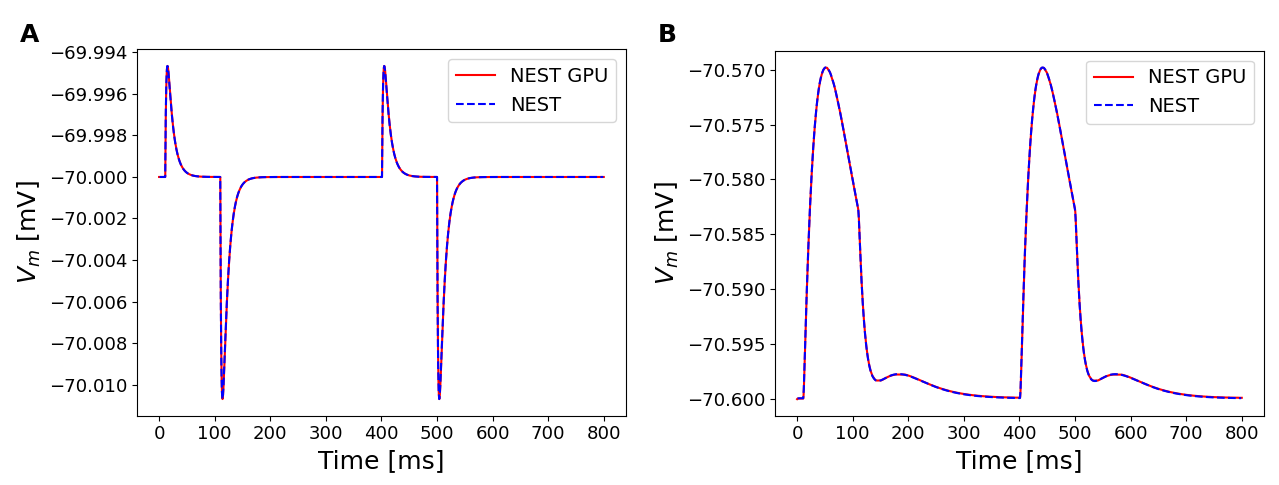
\includegraphics[width=\columnwidth]{figures/single_neurons.png}
    \caption{Membrane potentials of neurons injected with single spikes simulated using NEST (blue dotted line) and NEST GPU (red line). \textbf{(A)} LIF neuron with exponential current-based synapses. \textbf{(B)} AdEx neuron with conductance-based synapses and synaptic conductance modeled as an alpha function.}
    \label{fig:single_neurons_membrane_potential}
\end{figure}

Clearly, such a test is not enough to ensure the compatibility of NEST and NEST GPU. The following sections will describe the validation processes on the simulation of two large-scale network models, i.e., a cortical microcircuit model and a multi-area model.


\section{Simulations of the cortical microcircuit model}
\label{sec:cm_validation}
The first large-scale model that has been implemented in NEST GPU was the cortical microcircuit model of \cite{Potjans2012} described in Section \ref{sec:cortical_microcircuit}. It employs LIF neurons with exponential current-based synapses, which, as indicated in Figure \ref{fig:single_neurons_membrane_potential} do not show any relevant difference in the dynamic with respect to the NEST implementation. Indeed, this model is also integrated using the same integration method, which is the exact integration scheme proposed in \cite{Rotter1999}.\\
In order to validate the result of the NEST GPU simulations using NEST as a reference, we perform simulations using the Poisson spike generator as input for each area of the model, and we initialize the membrane potential following a normal distribution in order to avoid long transients. In addition, we perform a so-called pre-simulation phase of $500$\,ms without recording the spiking activity for the same reason. The simulation of the network dynamics (with enabled spike recording) is $600$\,s long, using a simulation time step of $0.1$\,ms. Indeed, such a long simulation of biological time to be simulated can be preferred, since it helps the activity statistics to converge, being able then to distinguish between the statistic of the spiking activity and random processes \cite{Dasbach2021}. Moreover, the full-scale simulation of such a model can be performed also using GPUs mounted in high-end laptops, since it requires a bit less than $4950$\,MiB of GPU memory and does not lead to an unmanageable amount of data to analyze.\\
Following the validation protocol discussed in Section \ref{sed:validation_protocol}, we compute the distributions of firing rate, CV ISI and Pearson correlation for all the $8$ populations of the model for NEST GPU and NEST and, to produce the distributions, we used the \texttt{seaborn.violinplot} function of the Seaborn Python library\cite{seaborn}, which returns KDE-smoothed optimized using the Silverman method, which is the same protocol we described in Section \ref{sec:KDE-EMD} for computing the distributions. Indeed, the first validation between NEST GPU and NEST, done in \cite{Golosio2021}, was not done using this package, but by extracting and smoothing the distributions autonomously trough our analysis script. By using the Seaborn Python library, we verified that the violin plot function uses the same protocol for binning and smoothing. Moreover, the violin plot has the advantage of showing side by side the distributions obtained using the two simulators, granting a better comparison of the results. Figure \ref{fig:violinplot_cm} shows the violin plot for a simulation of the cortical microcircuit model on NEST and NEST GPU.

\begin{figure}[H]
    \centering
    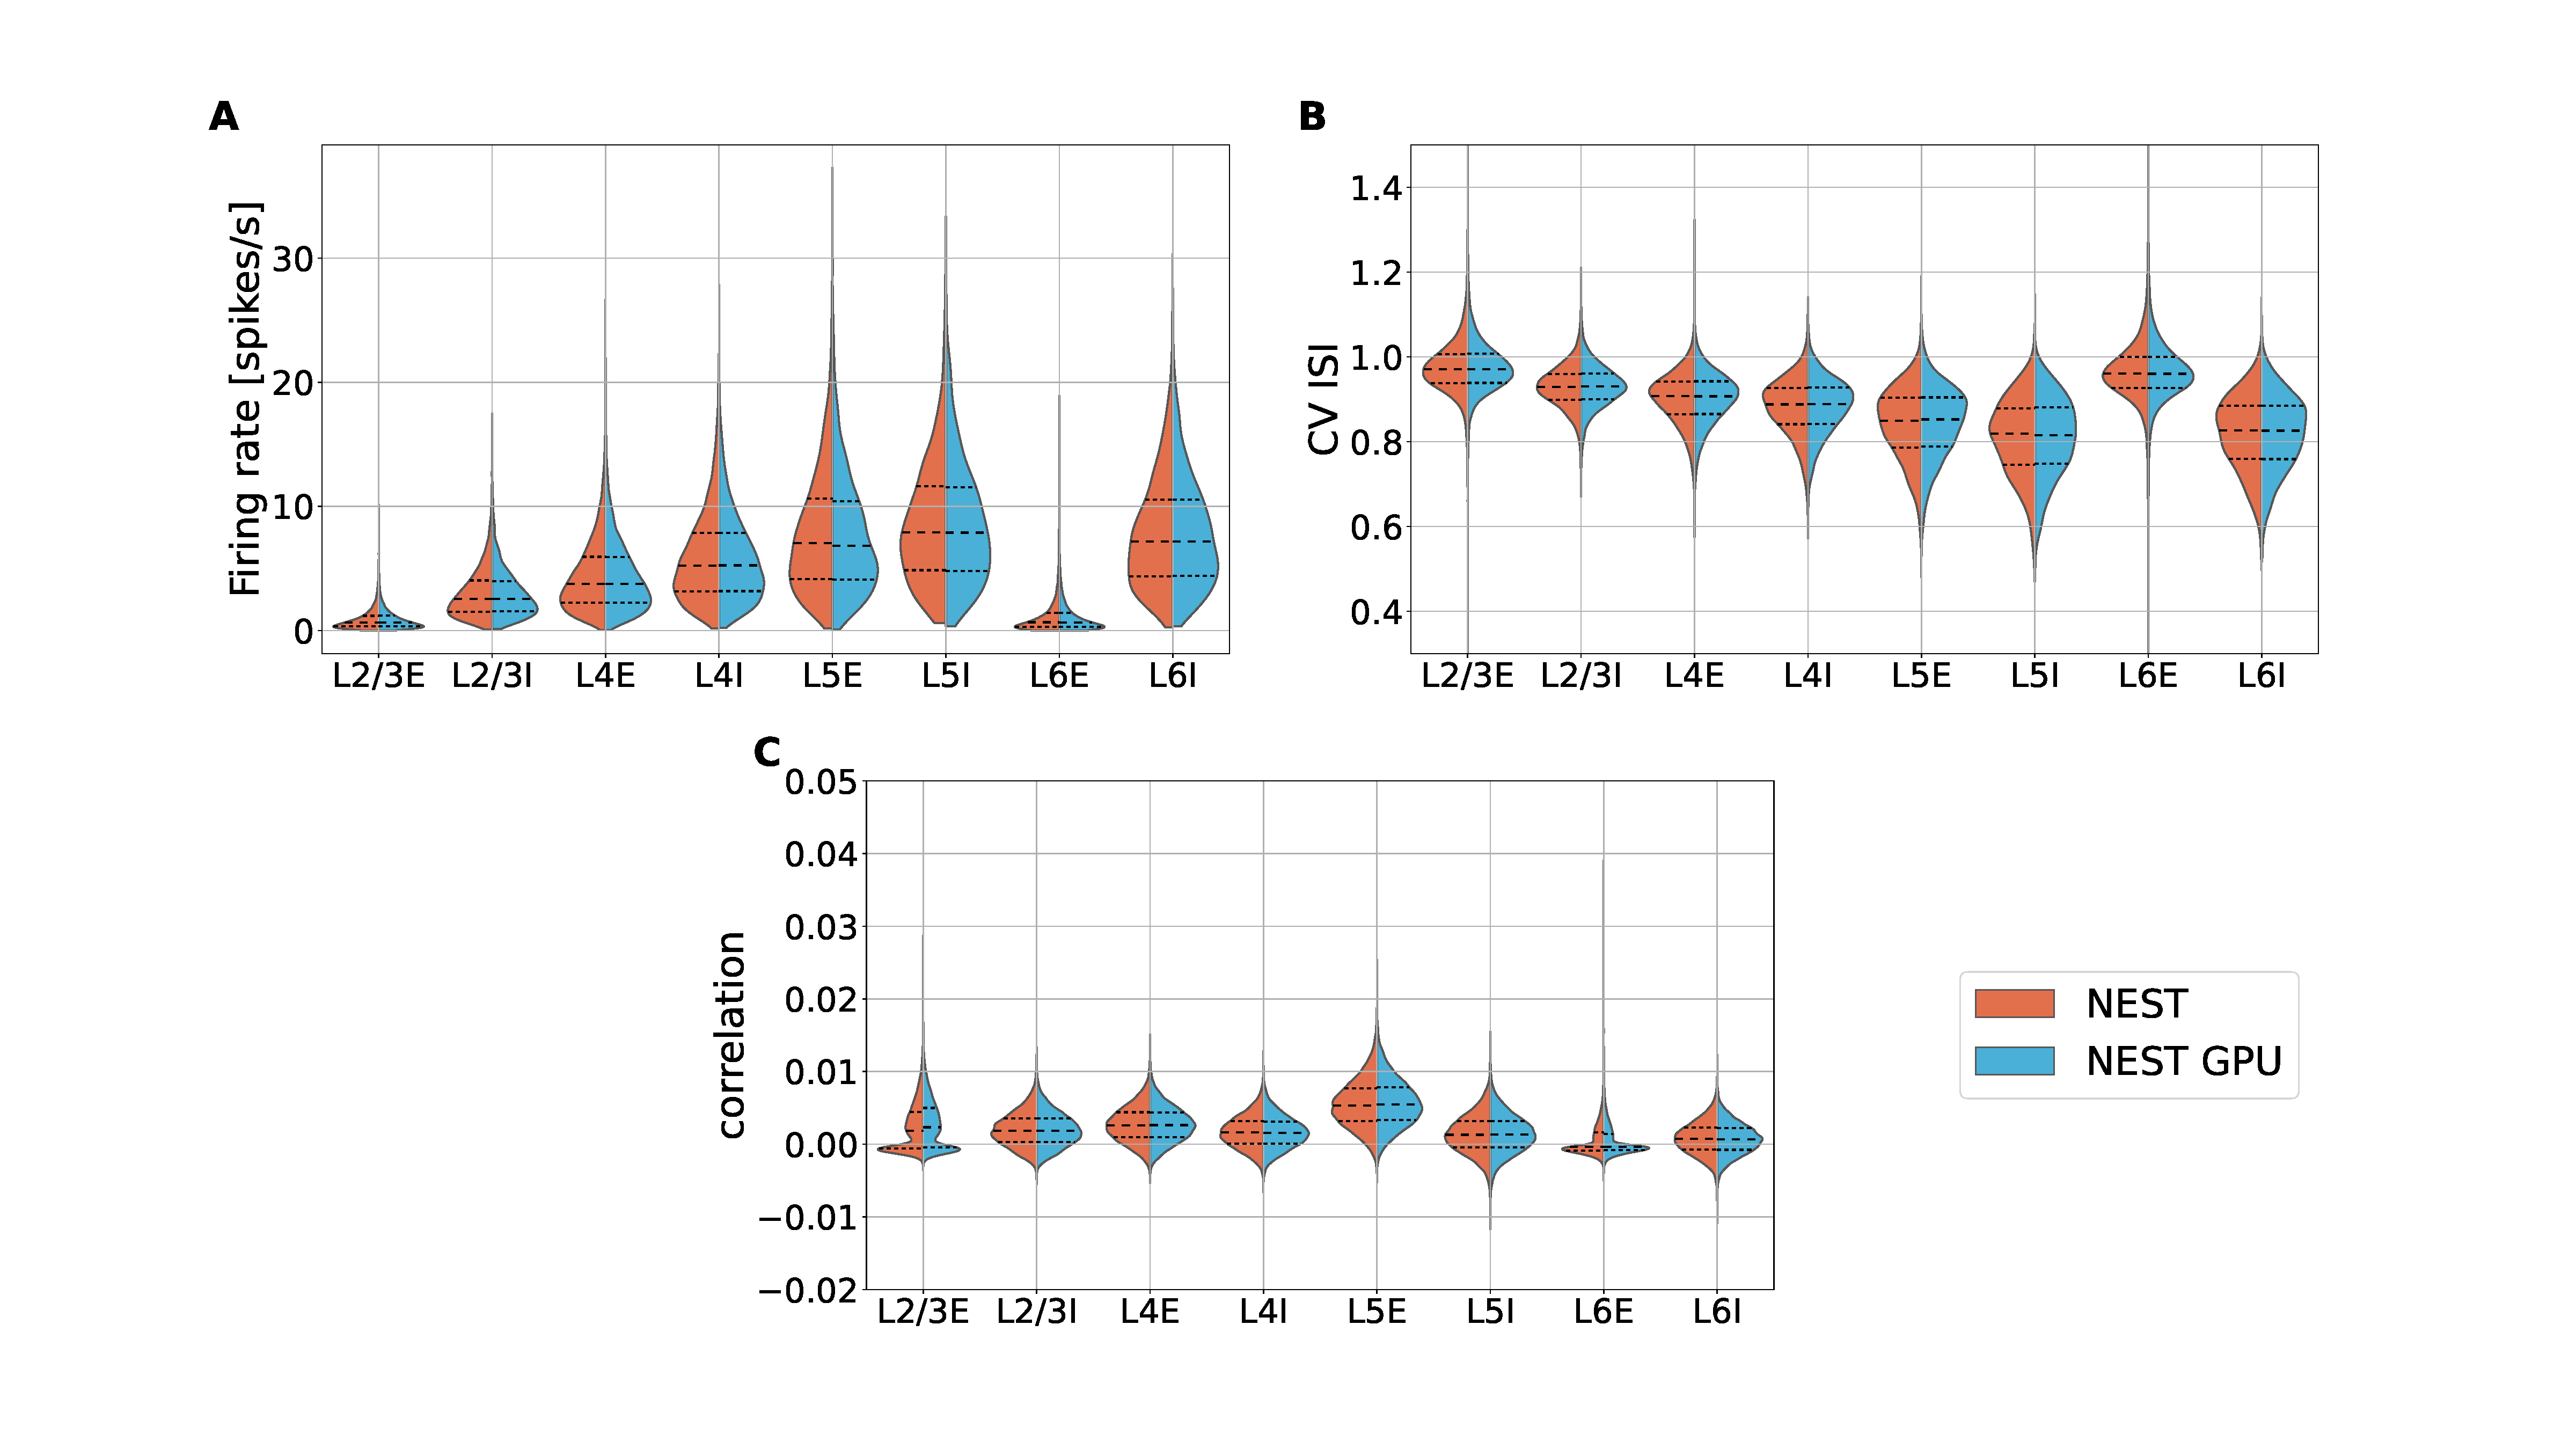
\includegraphics[trim=6cm 0 6cm 0, clip, width=\columnwidth]{figures/distributions_violinplot_cm_NEST_NGPU.pdf}
    \caption{Violin plot of the distributions of firing rate \textbf{(A)}, CV ISI \textbf{(B)} and Pearson correlation \textbf{(C)} extracted during a simulation of the cortical microcircuit model performed on NEST (orange distributions) and NEST GPU (sky blue distributions). Distributions are obtained for each population of the model, whose label is indicated in the abscissa. Central dashed line represent the median of the distribution, whereas the two side dashed lines represent the interquartile range.}
    \label{fig:violinplot_cm}
\end{figure}

As can be noticed, the distributions obtained with NEST and NEST GPU are visually indistinguishable. However, to provide also a quantitative estimation of the difference between the distribution, and compare the fluctuations between the two simulators and NEST with different seeds for random number generation, we computed the EMD. In this regard, we created three sets of $100$ simulations each using different seeds for random number generation, so that the comparison NEST-NEST and NEST-NEST GPU can be done. Figure \ref{fig:emd_cm} shows how values of EMD for such a comparison fluctuates for each population of the model and for each distribution obtained.

\begin{figure}[H]
    \centering
    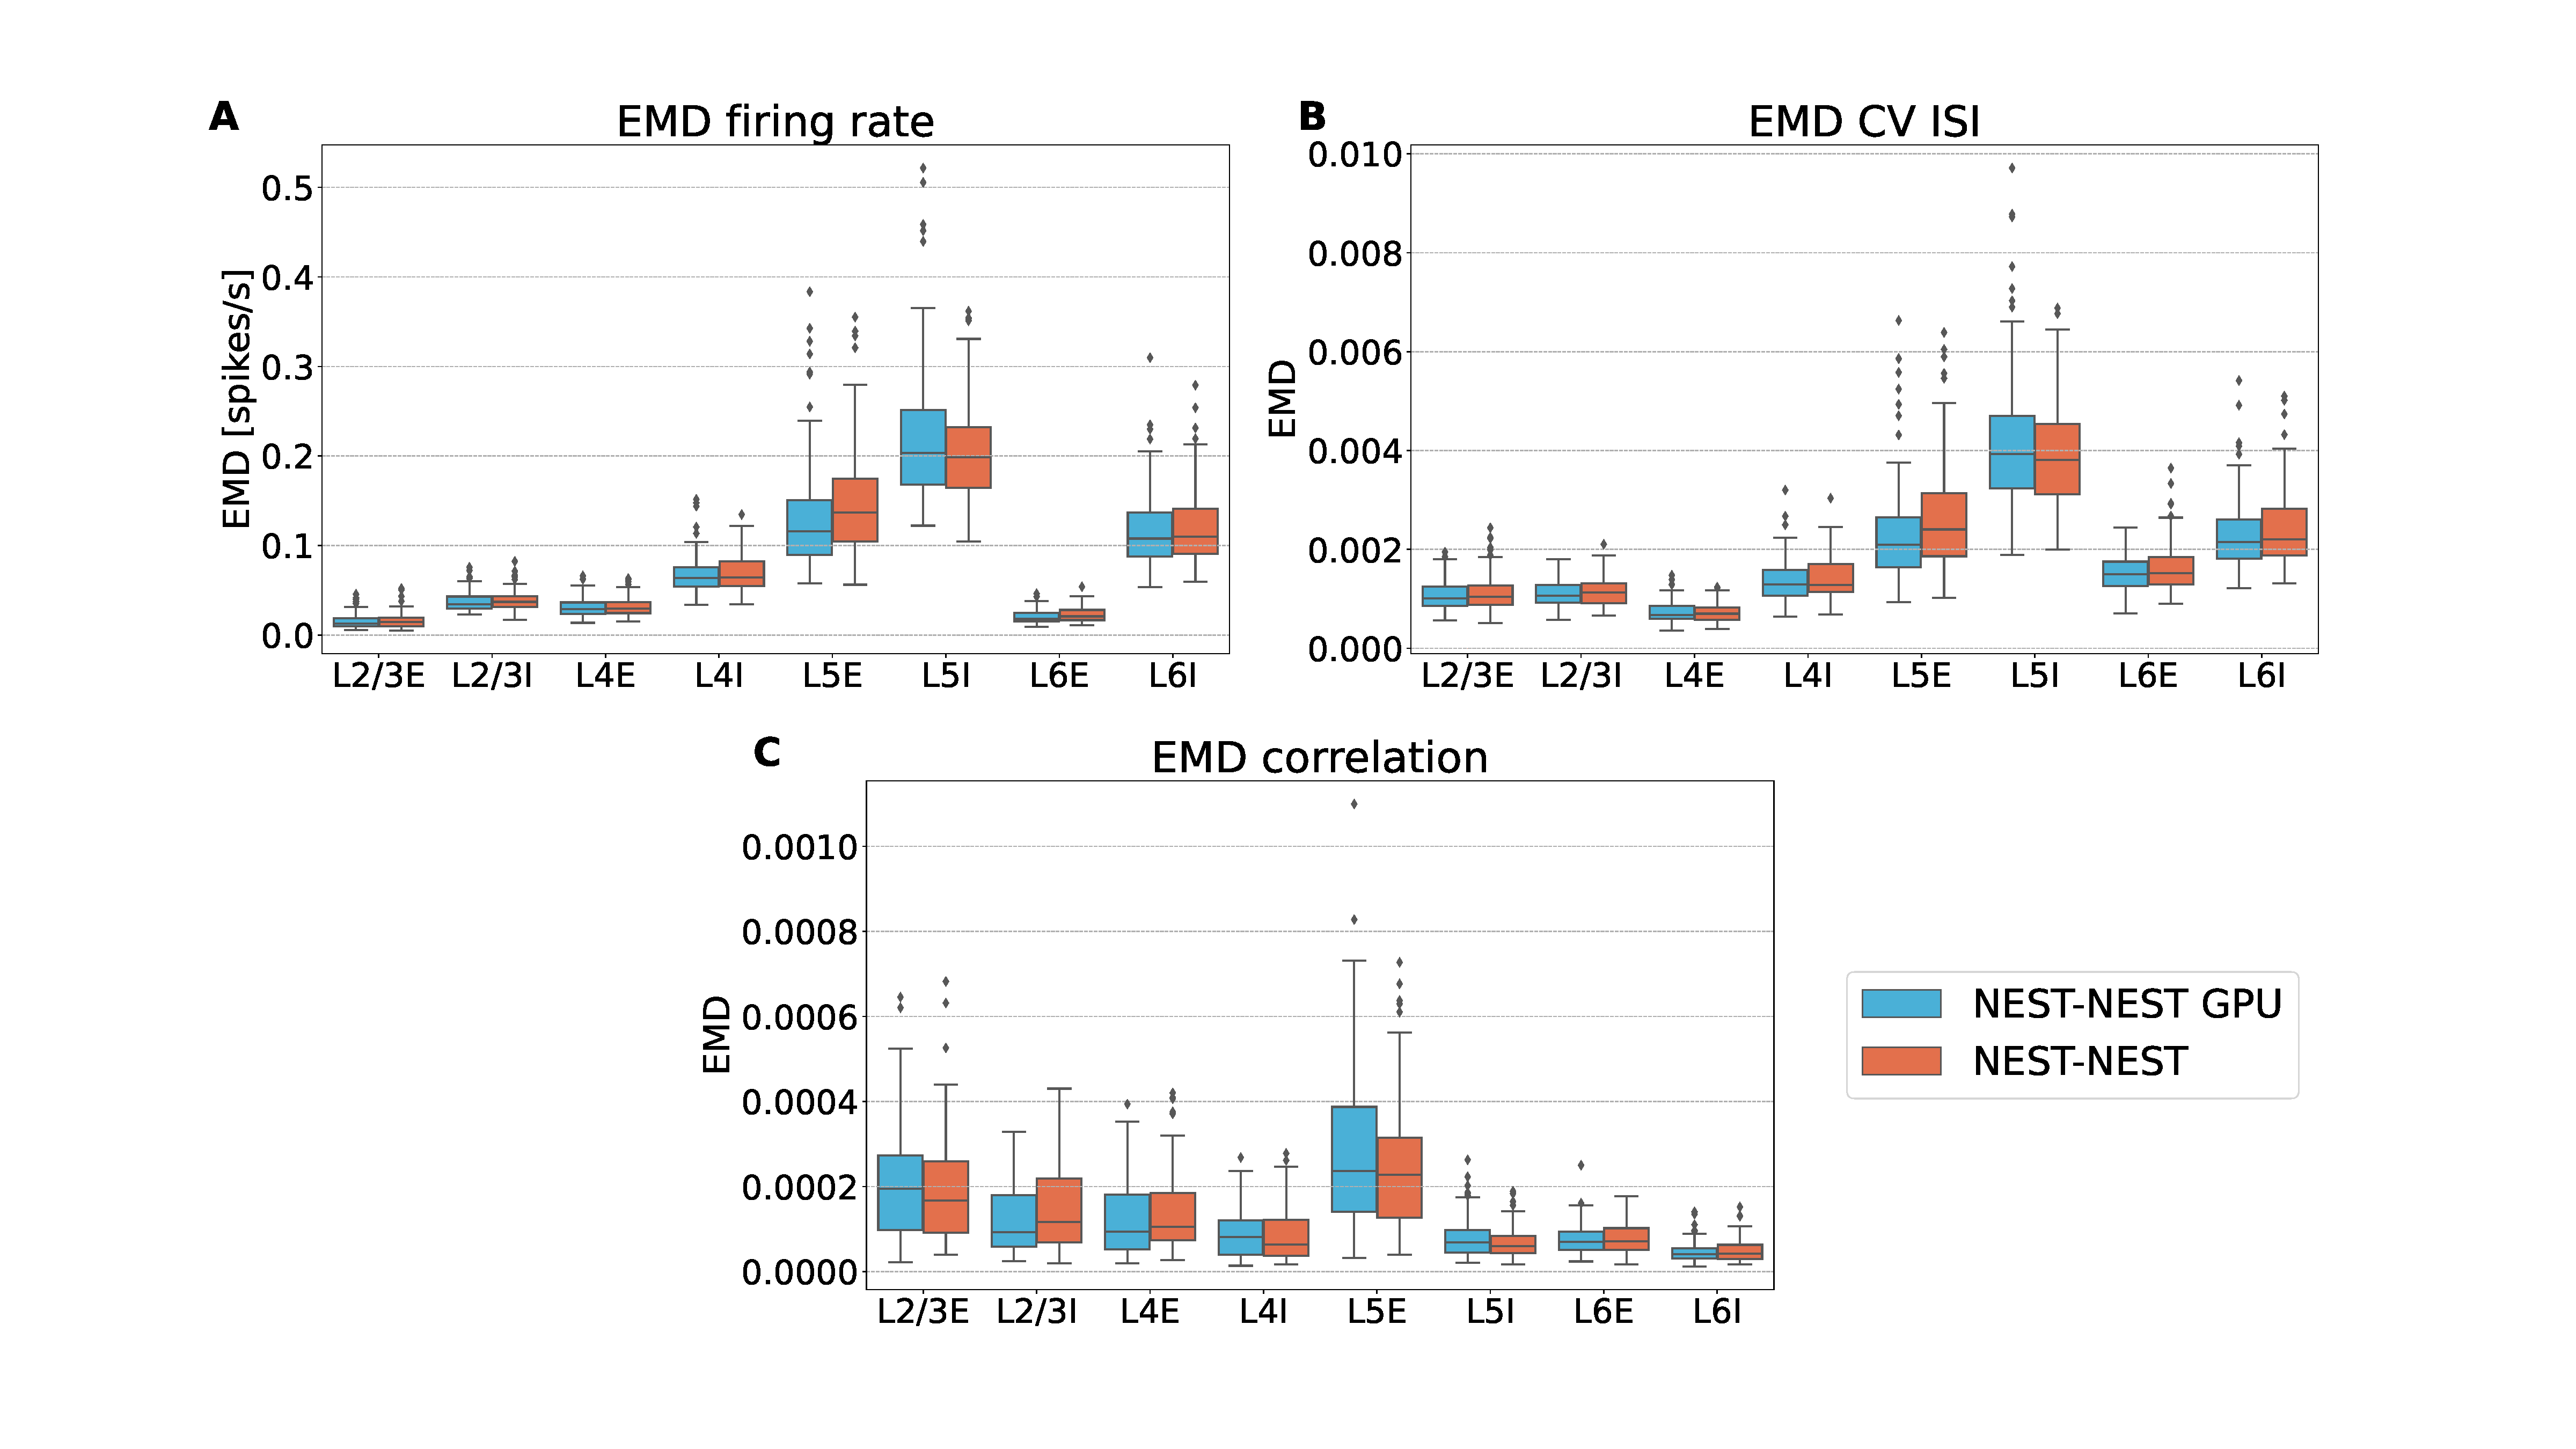
\includegraphics[trim=6cm 0 6cm 0, clip,width=\columnwidth]{figures/emd_boxplot_cm_NEST_NGPU.pdf}
    \caption{Box plots of the EMD obtained by comparing distributions of firing rate \textbf{(A)}, CV ISI \textbf{(B)} and Pearson correlation \textbf{(C)} for NEST and NEST GPU simulations (sky blue bars) or two sets of NEST simulations with different seeds (orange bars). Central line of the box plot represent the median of the distribution, whereas the extension of the boxes is determined by the interquartile range of the distribution formed by the values of EMD of each comparison. Whiskers shows the rest of the distribution as a function of the interquartile range, and dots represent the outliers.}
    \label{fig:emd_cm}
\end{figure}

Figure above, as previously discussed, compares the fluctuations we can expect by simulating the same model using two different simulators such as NEST and NEST GPU (i.e., NEST-NEST GPU comparison) and the ones we can have by comparing NEST simulations with different seeds for random number generation (i.e., NEST-NEST comparison). Thus, if the NEST-NEST GPU comparison fluctuates similarly with respect to the values of the NEST-NEST comparison, we can conclude that the usage of a different simulator does not have a significant variability when simulating the model, thus validating the simulator. In this case, we can notice that the fluctuations are totally compatible, and also the values of EMD are relatively low when compared to the values of the respective distributions in Figure \ref{fig:violinplot_cm}. Thus, we can affirm that NEST GPU is able to reproduce results statistically identical with respect of the ones of NEST.\\
The validation here reported compares the version 3.3 of NEST \cite{nest3.3} and the version of NEST GPU able to construct the network directly in the GPU memory, presented in \cite{Golosio2023} and available on the GitHub page of the library\footnote{\url{https://github.com/nest/nest-gpu}} under the git tag \texttt{nest-gpu\_onboard}\footnote{\url{https://github.com/nest/nest-gpu/releases/tag/nest-gpu_onboard}}.\\
Indeed, this validation workflow was employed for different versions of NEST and NEST GPU. For instance, in \cite{Golosio2021} was compared NEST version 2.20.0 \cite{nest2.20.0} and the prototype library NeuronGPU\footnote{\url{https://github.com/golosio/NeuronGPU}}. Moreover, during the development of the library, such a workflow is applied whenever a code modification results in a change of the spiking activity results, to ensure that the compatibility from a statistical point of view is always preserved.

\section{Simulations of the multi-area model}
In order to validate NEST GPU and the MPI implementation of its spike delivery algorithm, in \cite{Tiddia2022} we implemented and simulated the multi-area model of \cite{Schuecker2017, Schmidt2018b, Schmidt2018}. As described in Section \ref{sec:mam_description}, the model simulates 32 areas of the macaque visual cortex, each one represented by a patch of $1$\,mm$^2$ surface designed as the cortical microcircuit model of \cite{Potjans2012}. Thus, every area (except for the TH, which lacks of layer 4), has a total of 4 layers (i.e., 2/3, 4, 5, 6), each one having an excitatory (E) and an inhibitory (I) population.\\
In order to validate NEST GPU in the simulation of this model, we performed the same protocol described in Chapter \ref{chapter:models_and_validation} and applied in the previous section in the case of the cortical microcircuit model. However, some simulation parameters differ with respect of the validation workflow of the cortical microcircuit. For each set of simulation we performed $10$ simulations using different seed for random number generation. The pre-simulation time is set to $500$\,ms as well, however, we simulated $10$\,s of biological activity, using a simulation time step of $0.1$\,ms. The reason for the lower number of simulations and the shorter time of the simulation of the network dynamics is mainly linked to technical bottlenecks, mostly related to the limited compute time available to perform the simulations and the amount of data to be analyzed to produce the validation. Indeed, such a large-scale network, with about 4 million neurons and 24 billion synapses, requires a MPI-GPU cluster to be simulated, and in the case of these simulations we opted for a simulation using 32 compute nodes, each equipped with a GPU device. Details on the computing platform used to perform the simulations will be provided in the next chapter.\\
As mentioned in Section \ref{sec:mam_description}, the multi-area model can exhibit two activity states: a stationary ground state with relatively low firing rate variability and a metastable state, more realistic and with an increase in the rate fluctuation and inter-area interactions. As a reference, Figure \ref{fig:raster_plot_mam} shows the raster plot of two of the 32 areas of the model to show the difference in the spiking activity between these states.

\begin{figure}[H]
    \centering
    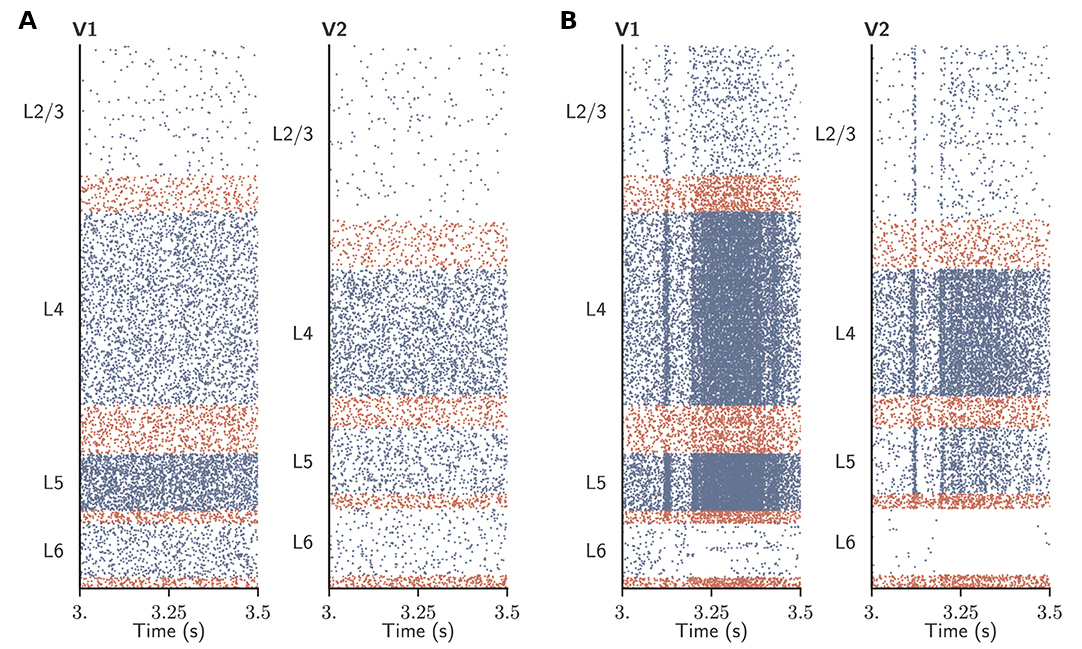
\includegraphics[width=\columnwidth]{figures/raster_plot_mam.jpg}
    \caption{Raster plot for the areas V1 and V2 of the multi-area model when the network is in the ground state \textbf{(A)} and in the metastable state \textbf{(B)}. Figure adapted from \cite{Tiddia2022}.}
    \label{fig:raster_plot_mam}
\end{figure}

As can be seen, raster plot of the ground state of the model show a behavior without significant changes of the network activity, whereas the metastable state is quite the opposite. It should be noted that the only difference between the two states of the model is the strength of the cortico-cortical synapses: when the strength is the same with respect to the intra-area synapses the model is in its ground state, whereas the metastable state have the strength of the cortico-cortical connections increased.\\
For the purpose of this study, we validated both the ground state and the metastable state of the model. We computed the distributions of firing rate, CV ISI and Pearson correlation for each population of the model, so that for each state we extracted a total of $762$ distributions ($254$ distributions per statistical measure). Distributions were smoothed trough the KDE with a Gaussian kernel using a bandwidth driven by the Silverman method. As explained in the previous section, such a task can be done by the Seaborn \texttt{violinplot} function, which is useful to compare at first glance distributions obtained, in this case, using NEST and NEST GPU.\\
Figure \ref{fig:mam_sample_dist} represents the violin plots of firing rate, CV ISI and Pearson correlation obtained from a simulation of the multi-area model using NEST and NEST GPU for the first area of the model (i.e., V1) in the ground and metastable state. This is depicted as a sample, however, the distributions for all the populations and areas of the model are shown in Appendix \ref{app:mam_validation}.

\begin{figure}[H]
    \centering
    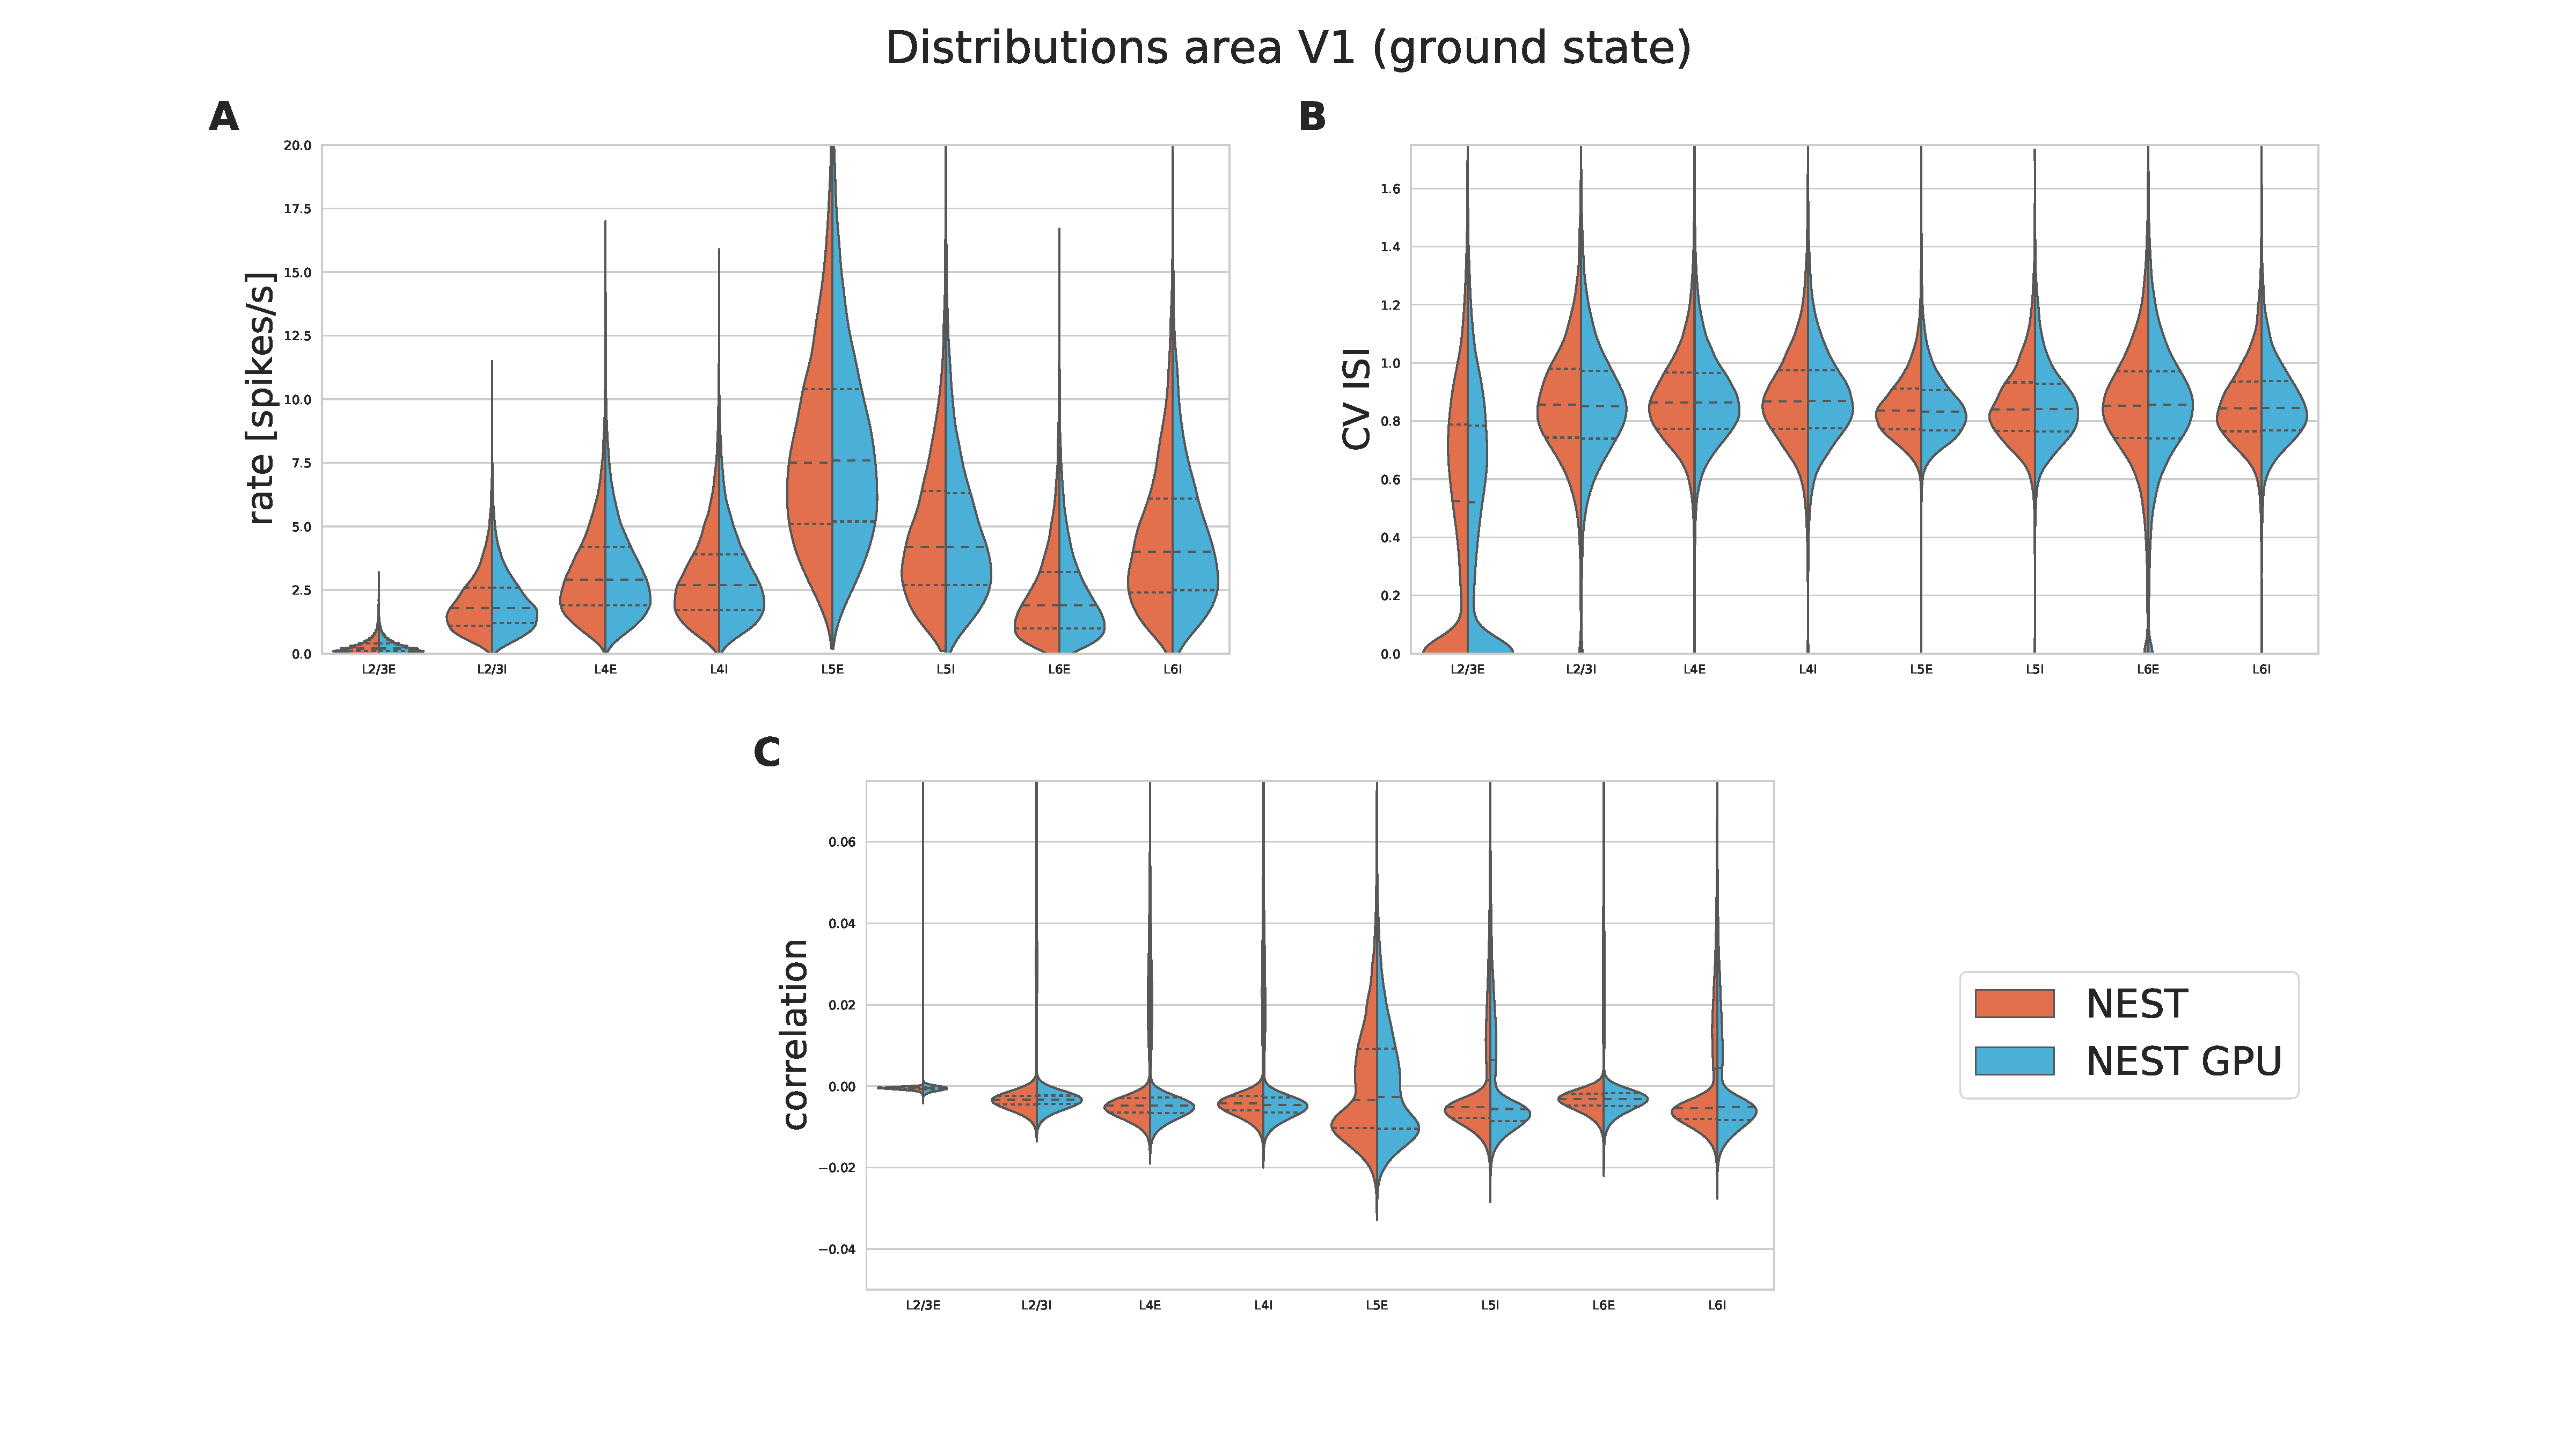
\includegraphics[trim=6cm 0 6cm 0, clip,width=\columnwidth]{figures/dist_violinplot_sample_gs.pdf}
    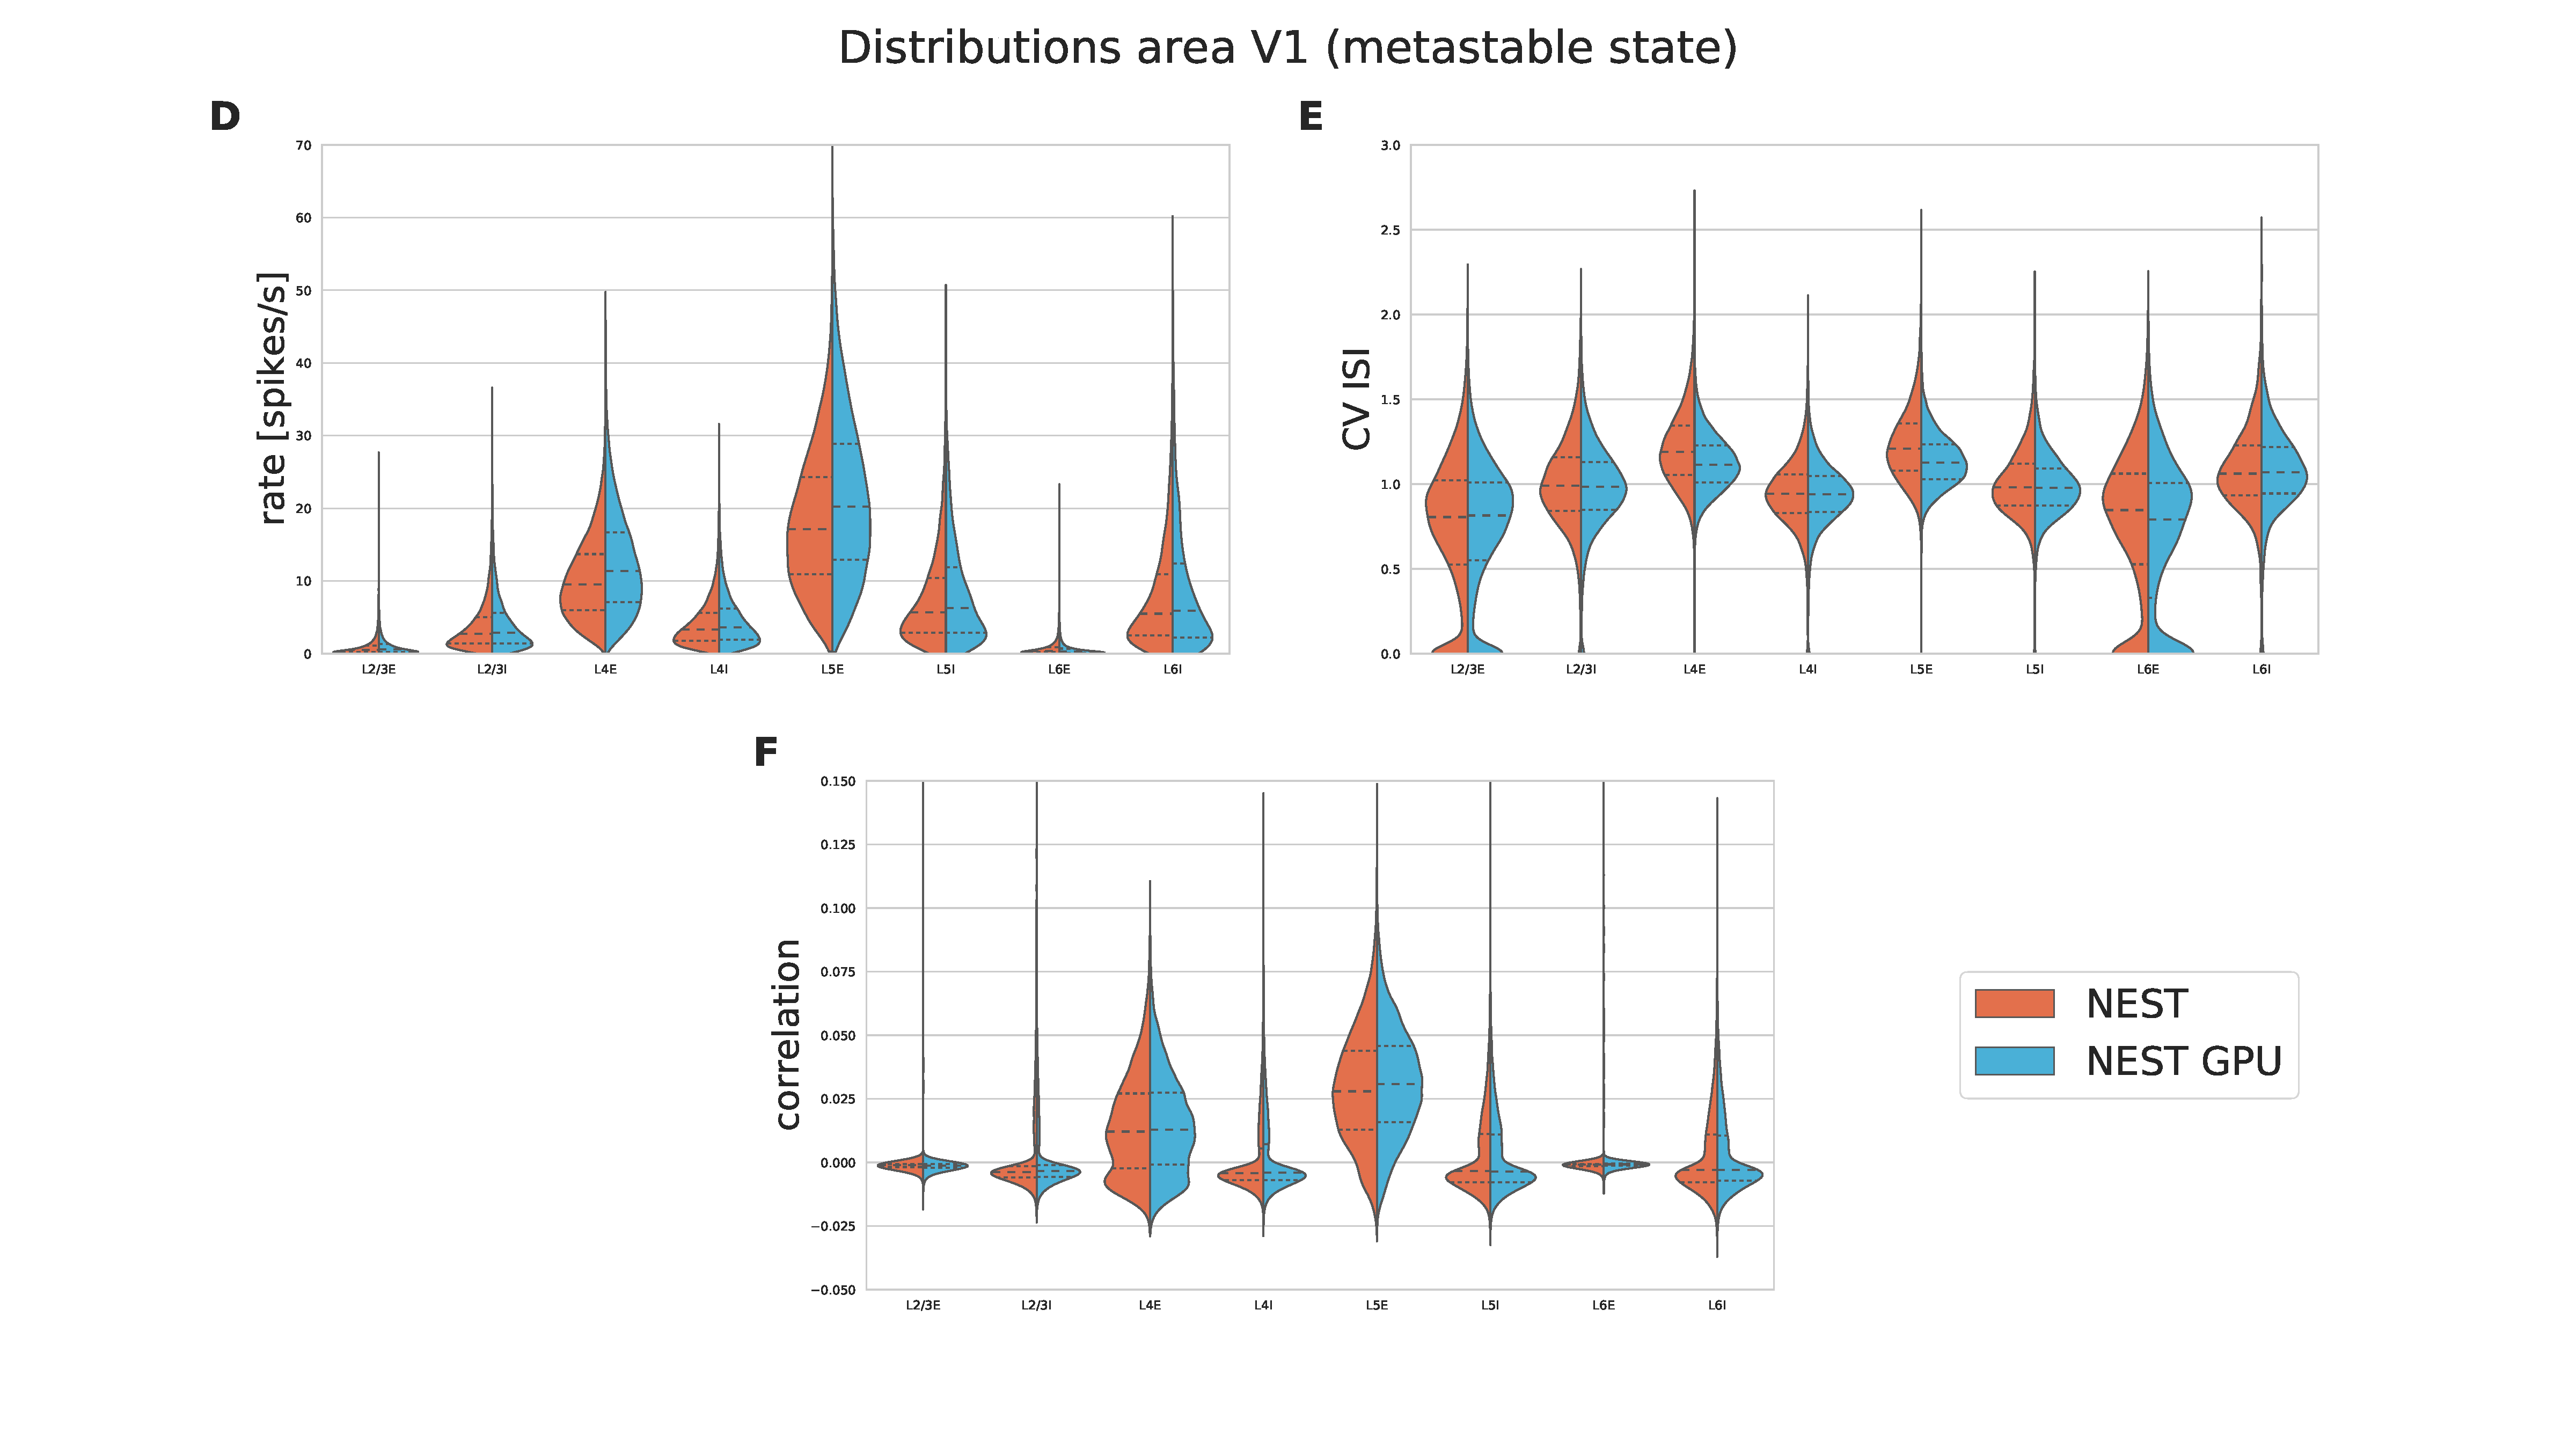
\includegraphics[trim=6cm 0 6cm 0, clip,width=\columnwidth]{figures/dist_violinplot_sample_ms.pdf}
    \caption{Violin plot of the distributions of firing rate, CV ISI and Pearson correlation extracted during a simulation of the multi-area model of the ground state (\textbf{A,B,C}) and the metastable state (\textbf{D,E,F}) for the area V1. Simulations are performed on NEST (orange distributions) and NEST GPU (sky blue distributions). Central dashed line represent the median of the distributions, the other two dashed lines represent the interquartile range.}
    \label{fig:mam_sample_dist}
\end{figure}

As can be noticed, the distributions of NEST and NEST GPU are barely indistinguishable when simulating the ground state of the multi-area model.\\
Indeed, in the distributions of metastable state of the model, we can notice, apart from higher rates and variability indicated by the values of the statistical distributions, a larger difference between NEST and NEST GPU distributions, so that the distributions are not indistinguishable as in the case of the ground state. However, we have to consider that, in such a state, even a change of the seed for random number generation can lead to an large variability with respect to what we observe in the ground state. To make this clear, Figure \ref{fig:sample_mam_gs} and \ref{fig:sample_mam_ms} show the distributions of firing rate, CV ISI and Pearson correlation just for two populations of the area V1 of the model in both the ground state and the metastable state. NEST and NEST GPU distributions are shown not using the violin plot function but using our analysis workflow that produces smoothed distributions without employing the Seaborn \texttt{violinplot} function. Moreover, to underline the variability due to the change of seed, here we show distributions averaged over the $10$ seeds of random number generation employed, together with the standard deviation of the mean.


As can be seen, metastable state simulations have a higher variability even when the seed is changed using the same simulator. In this regard, the usage of EMD to compare the fluctuations when using the simulators can be particularly useful, since it is not trivial to ensure the compatibility between NEST and NEST GPU. Thus, having 2 sets of NEST simulations and a set of NEST GPU simulations using 10 different seeds for random number generation, we perform 10 pairwise comparisons between NEST and NEST GPU and 10 comparisons between the two sets of NEST simulations. The EMD values related to these comparisons are then collected in box plots and plotted side by side for a more effective comparison of the fluctuations driven by the usage of a different seed and the ones driven by the usage of a different simulator.\\
Figure \ref{fig:mam_sample_emd} shows the EMD box plots for the comparison of, respectively, firing rate, CV ISI and Pearson correlation distributions for each population and area of the multi-area model in the case of ground state and metastable state simulations.


\begin{figure}[H]
    \centering
    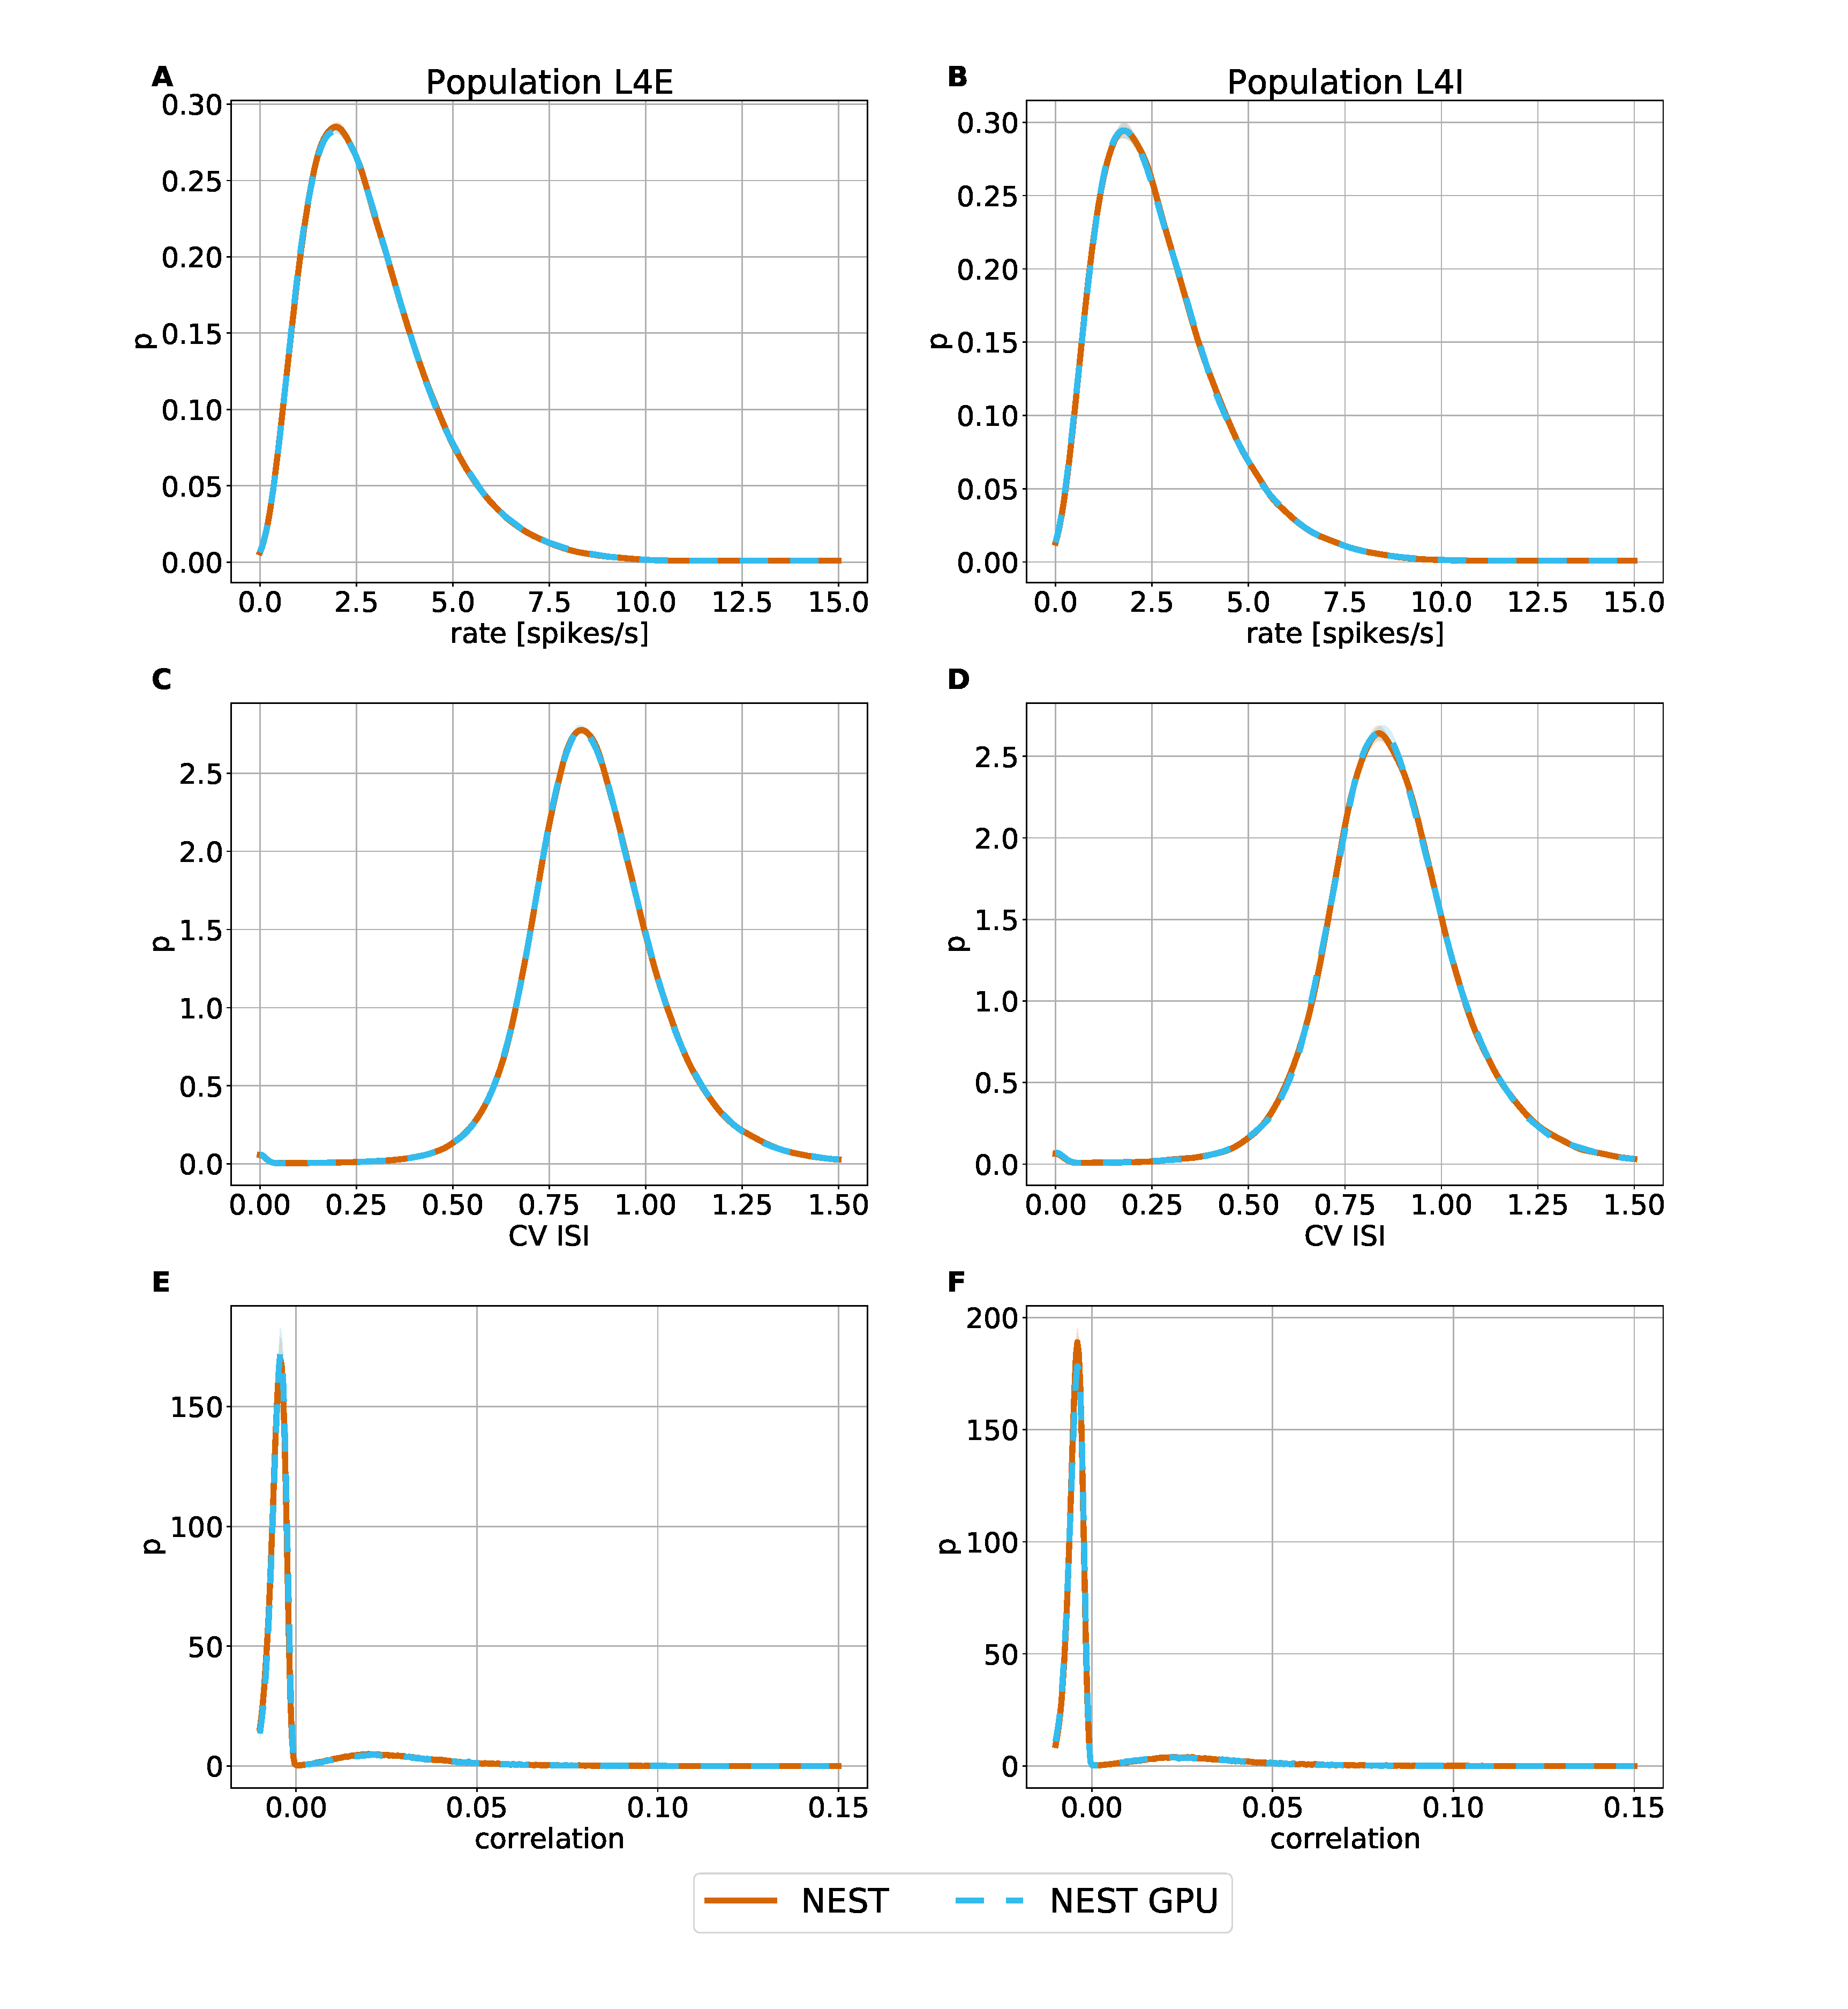
\includegraphics[trim=3cm 0 3cm 0, clip,width=\columnwidth]{figures/sample_gs.pdf}
    \caption{Ground state distributions of firing rate 
    \textbf{(A,B)}, CV ISI \textbf{(C,D)} and Pearson correlations \textbf{(E,F)} for the populations L4E and L4I of the area V1 of the multi-area model. Distributions are averaged over 10 simulations with NEST (orange line) and NEST GPU (sky blue dotted line). Sky blue and orange shading represent the standard deviation of the distributions. Figure adapted from \cite{Tiddia2022}.}
    \label{fig:sample_mam_gs}
\end{figure}

\begin{figure}[H]
    \centering
    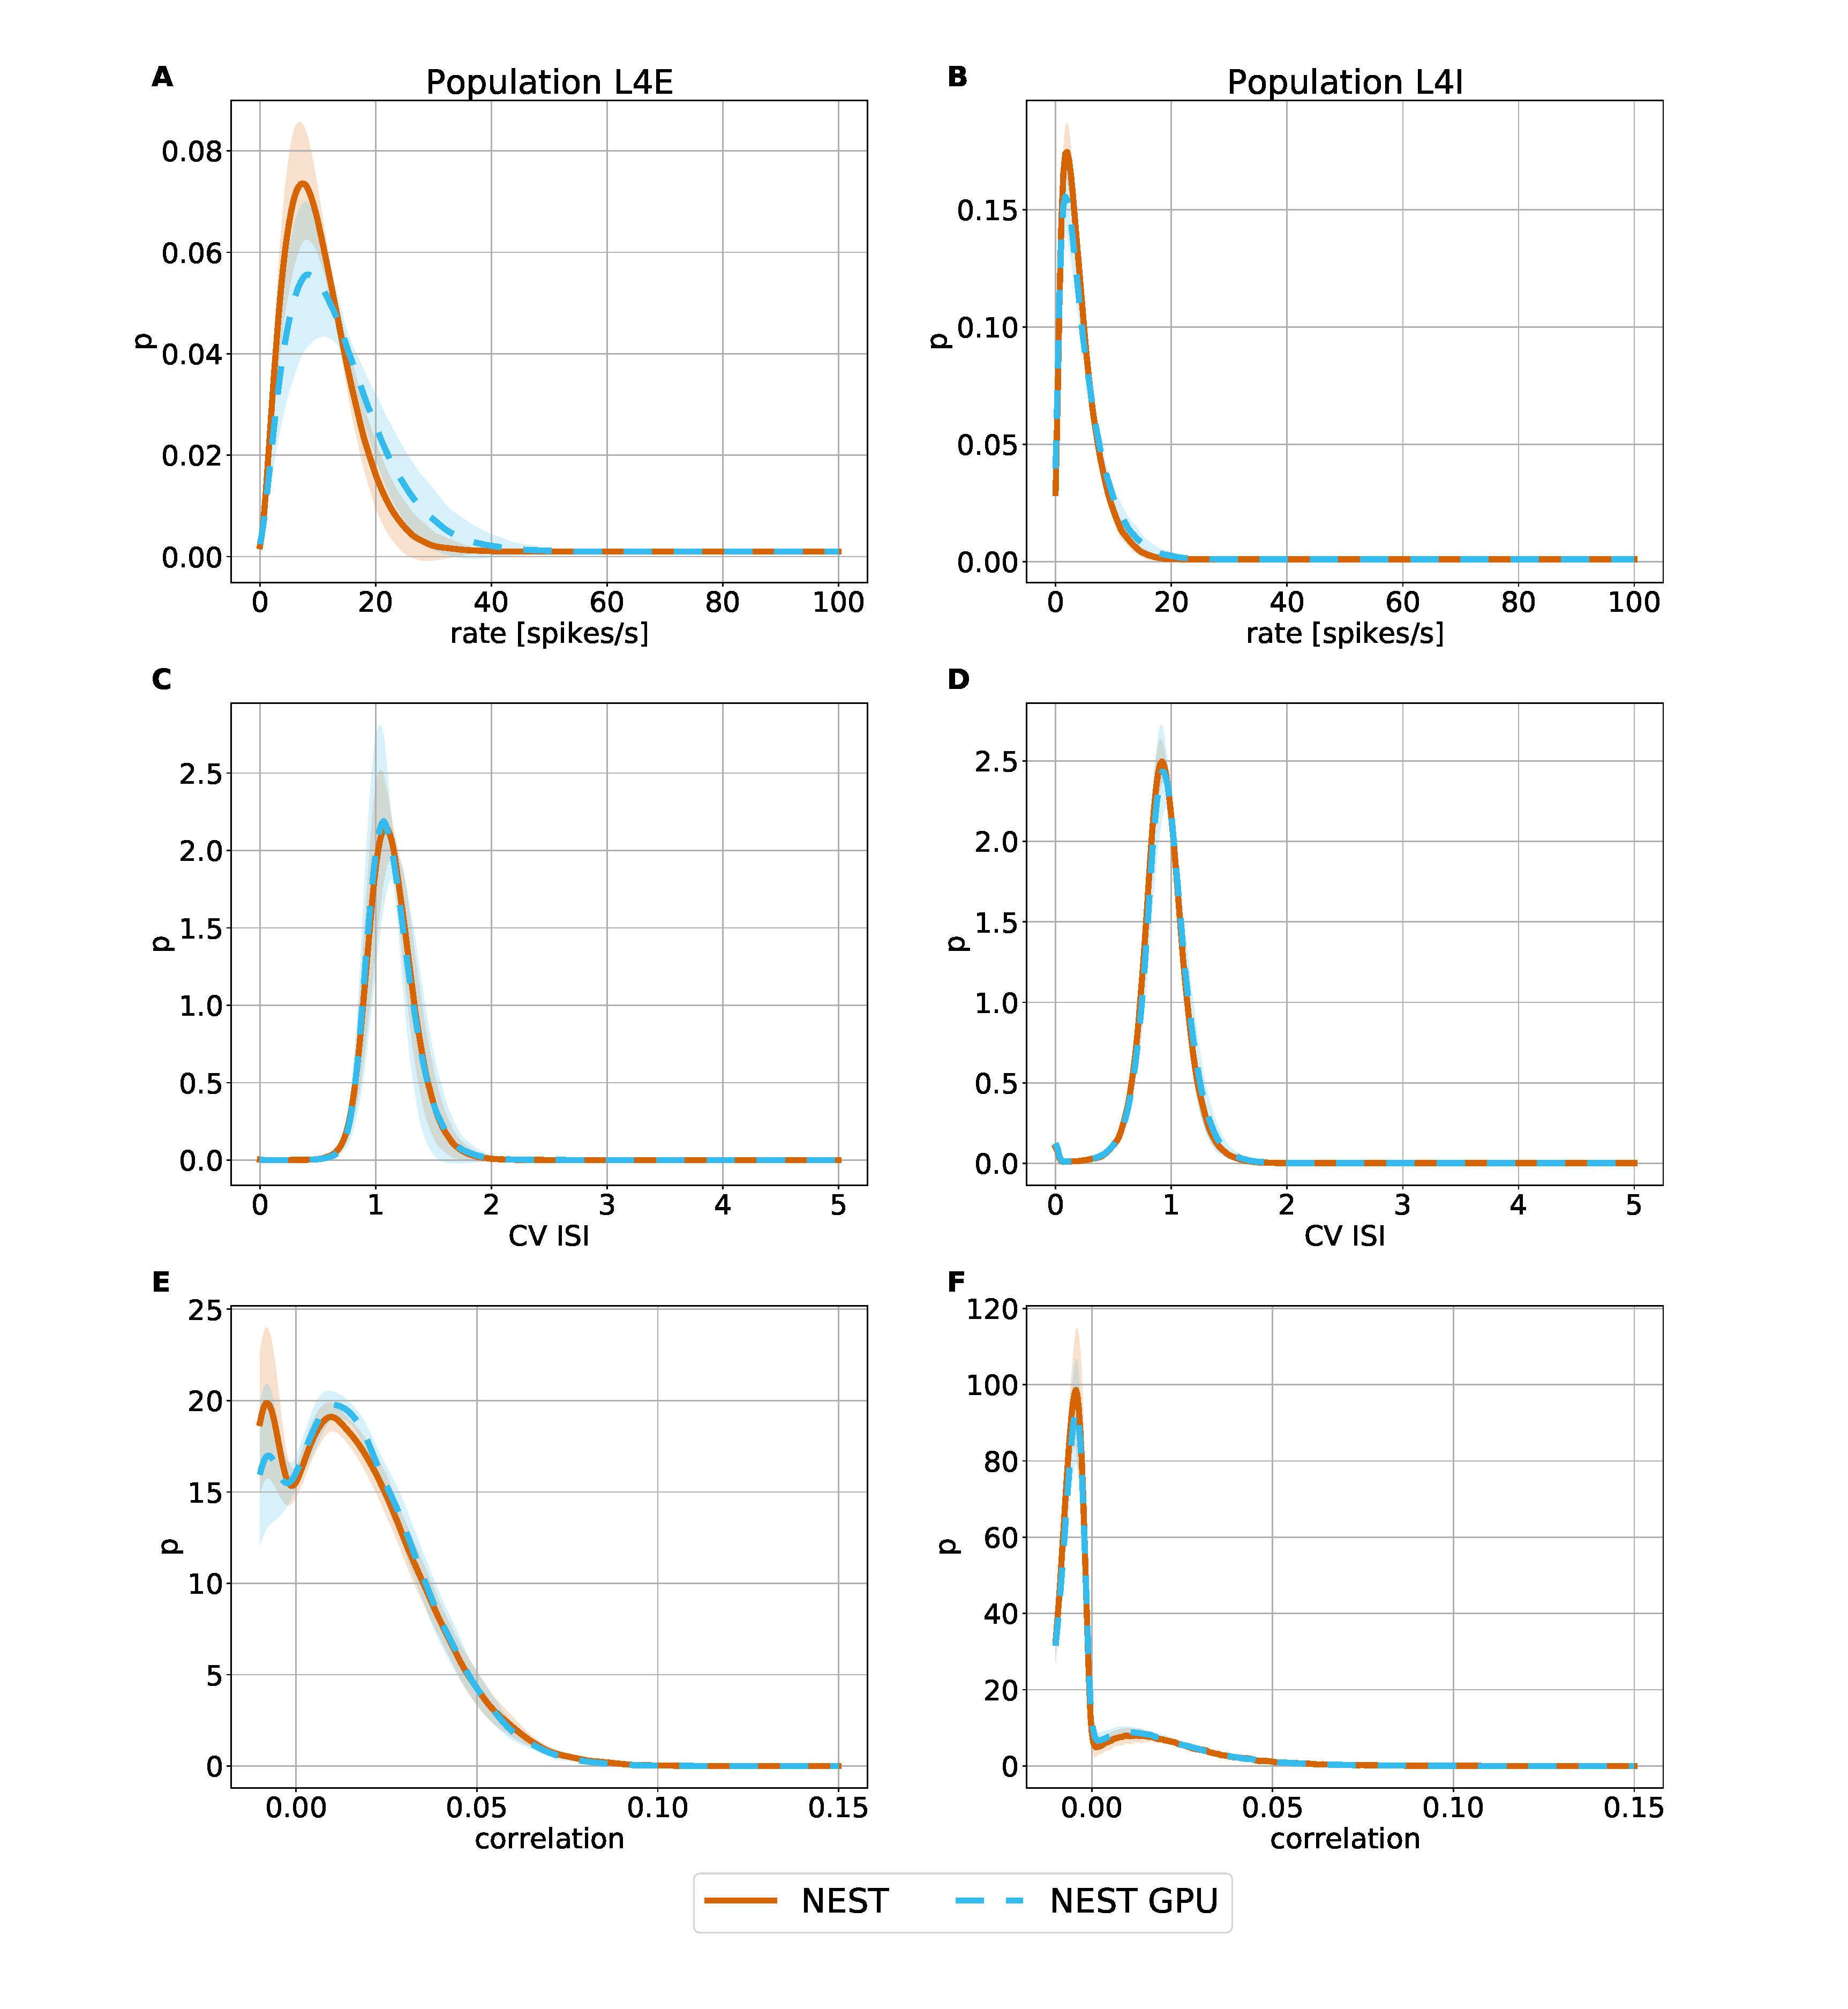
\includegraphics[trim=3cm 0 3cm 0, clip,width=\columnwidth]{figures/sample_ms.pdf}
    \caption{Metastable state distributions of firing rate 
    \textbf{(A,B)}, CV ISI \textbf{(C,D)} and Pearson correlations \textbf{(E,F)} for the populations L4E and L4I of the area V1 of the multi-area model. Distributions are averaged over 10 simulations with NEST (orange line) and NEST GPU (sky blue dotted line). Sky blue and orange shading represent the standard deviation of the distributions. Figure adapted from \cite{Tiddia2022}.}
    \label{fig:sample_mam_ms}
\end{figure}

\begin{figure}[H]
    \centering
    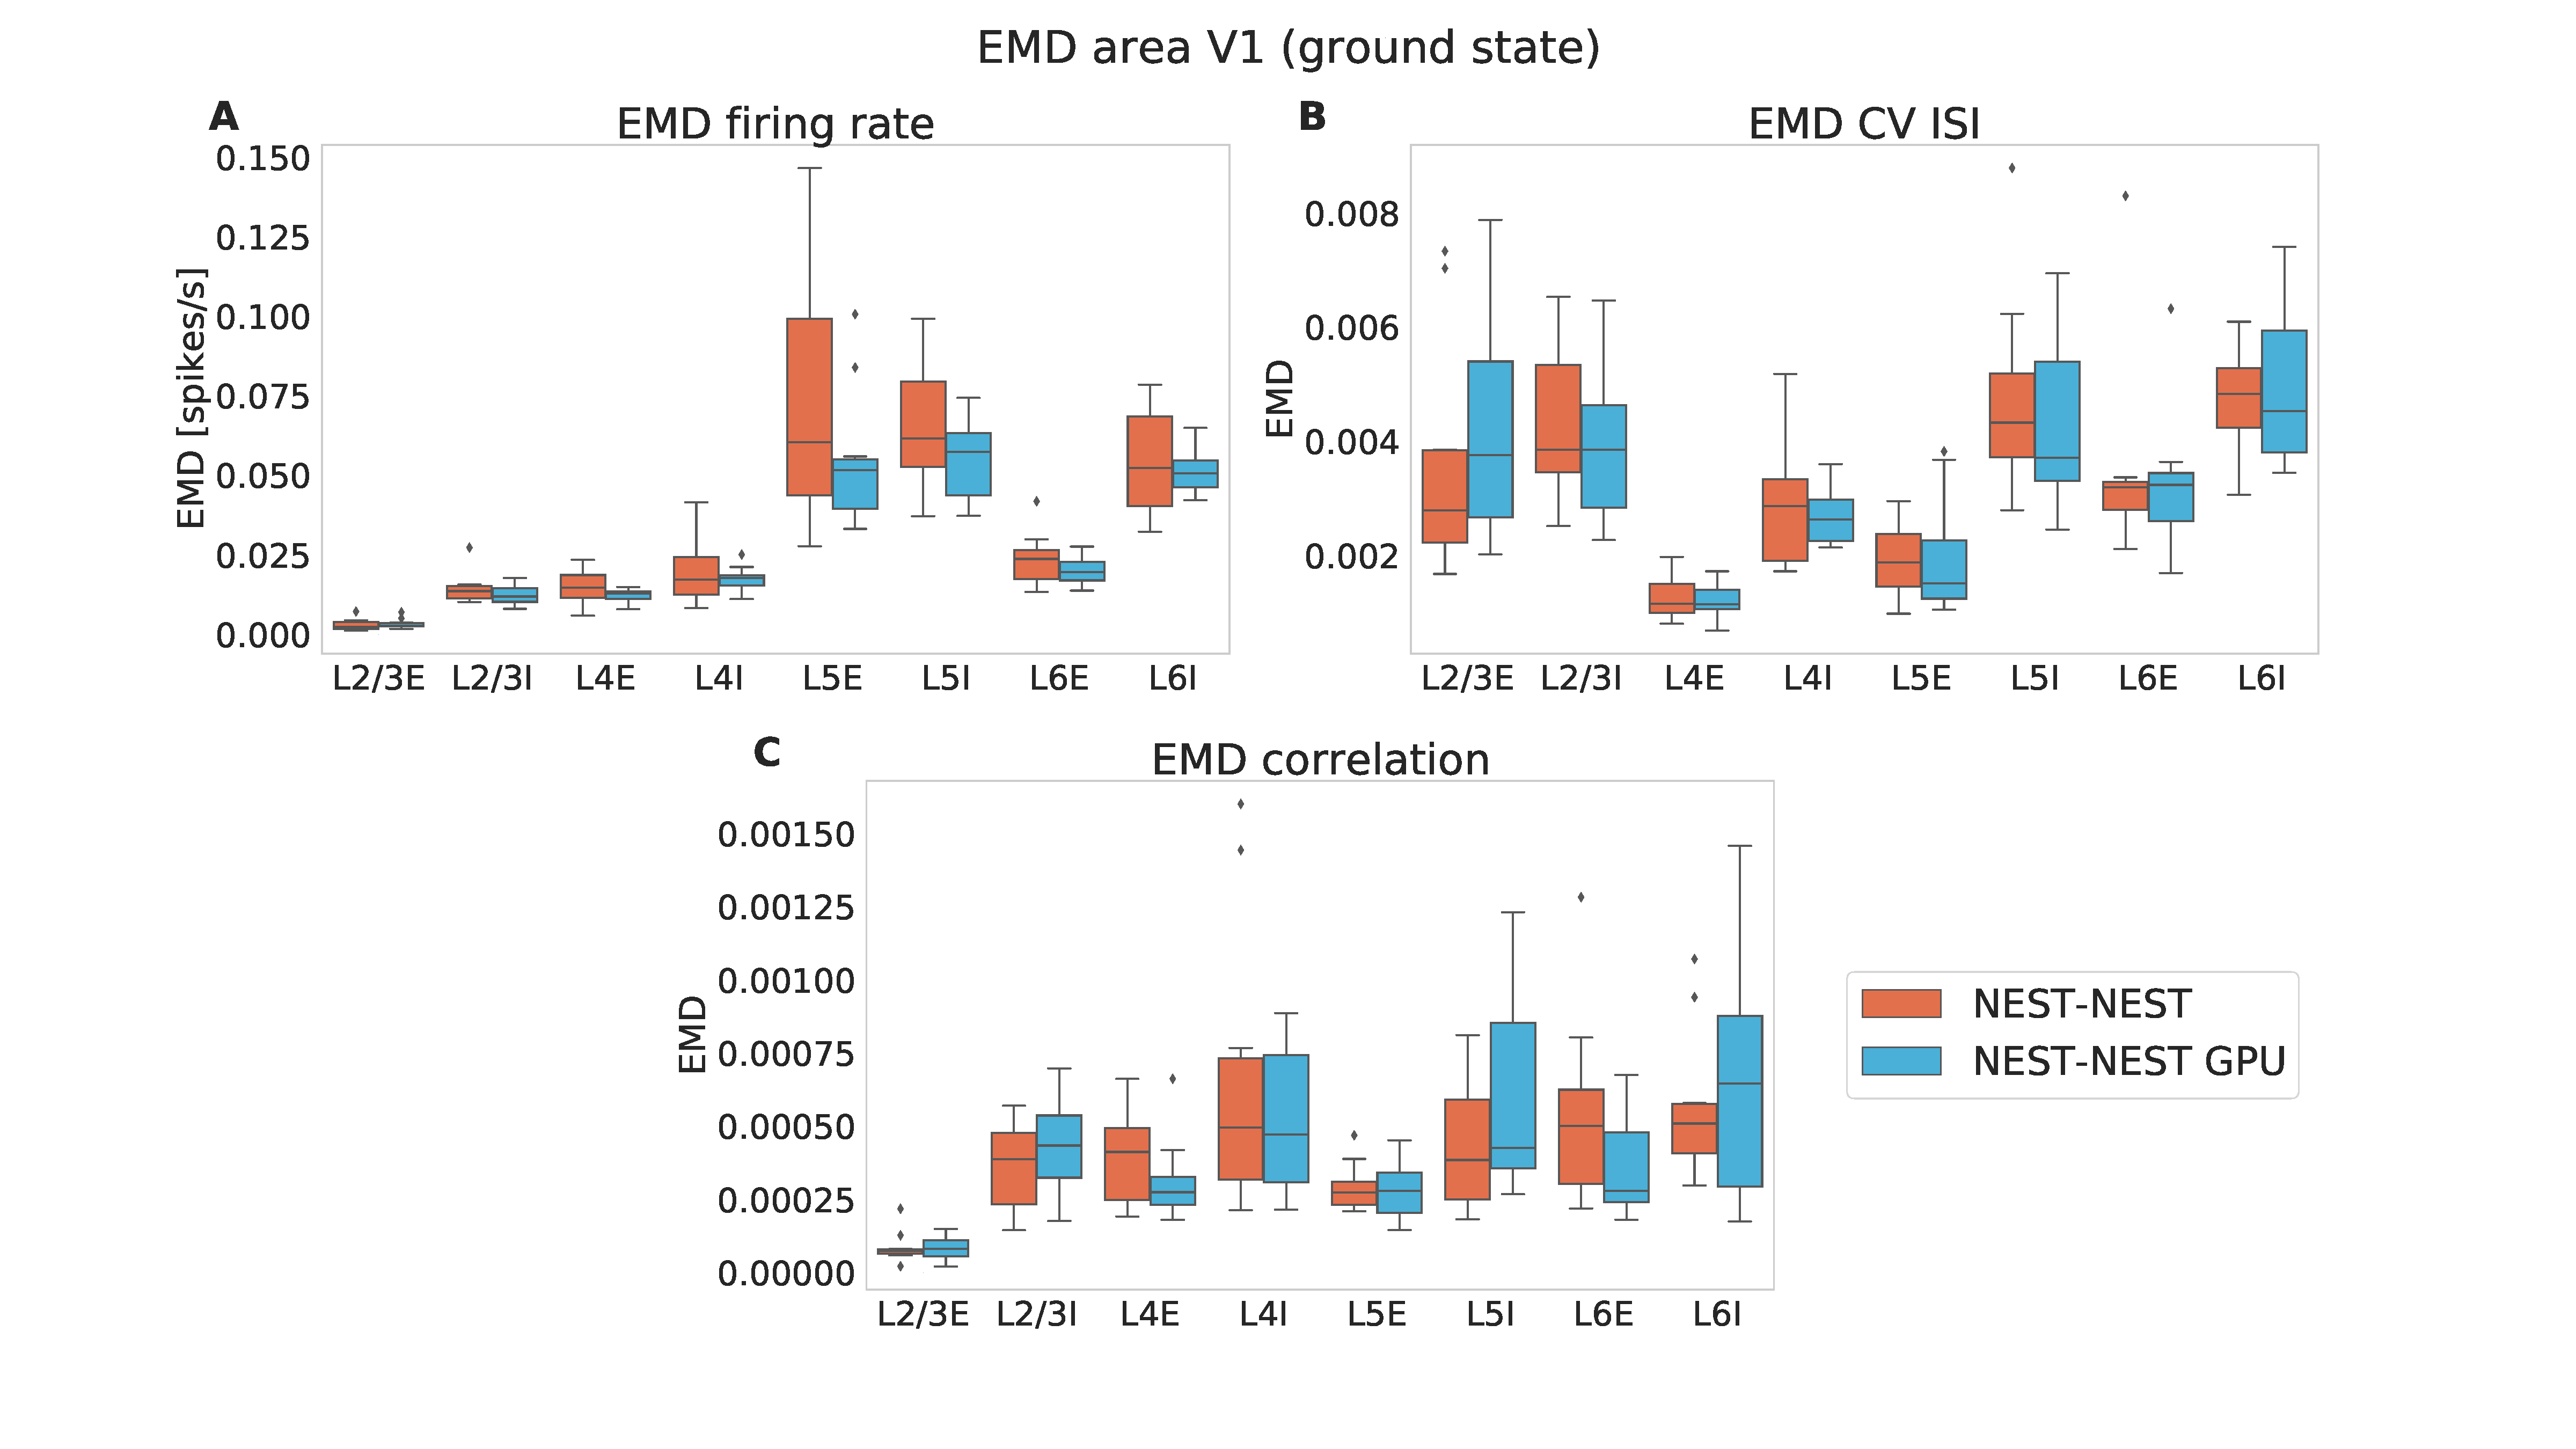
\includegraphics[trim=6cm 0 6cm 0, clip,width=\columnwidth]{figures/emd_boxplot_sample_gs.pdf}
    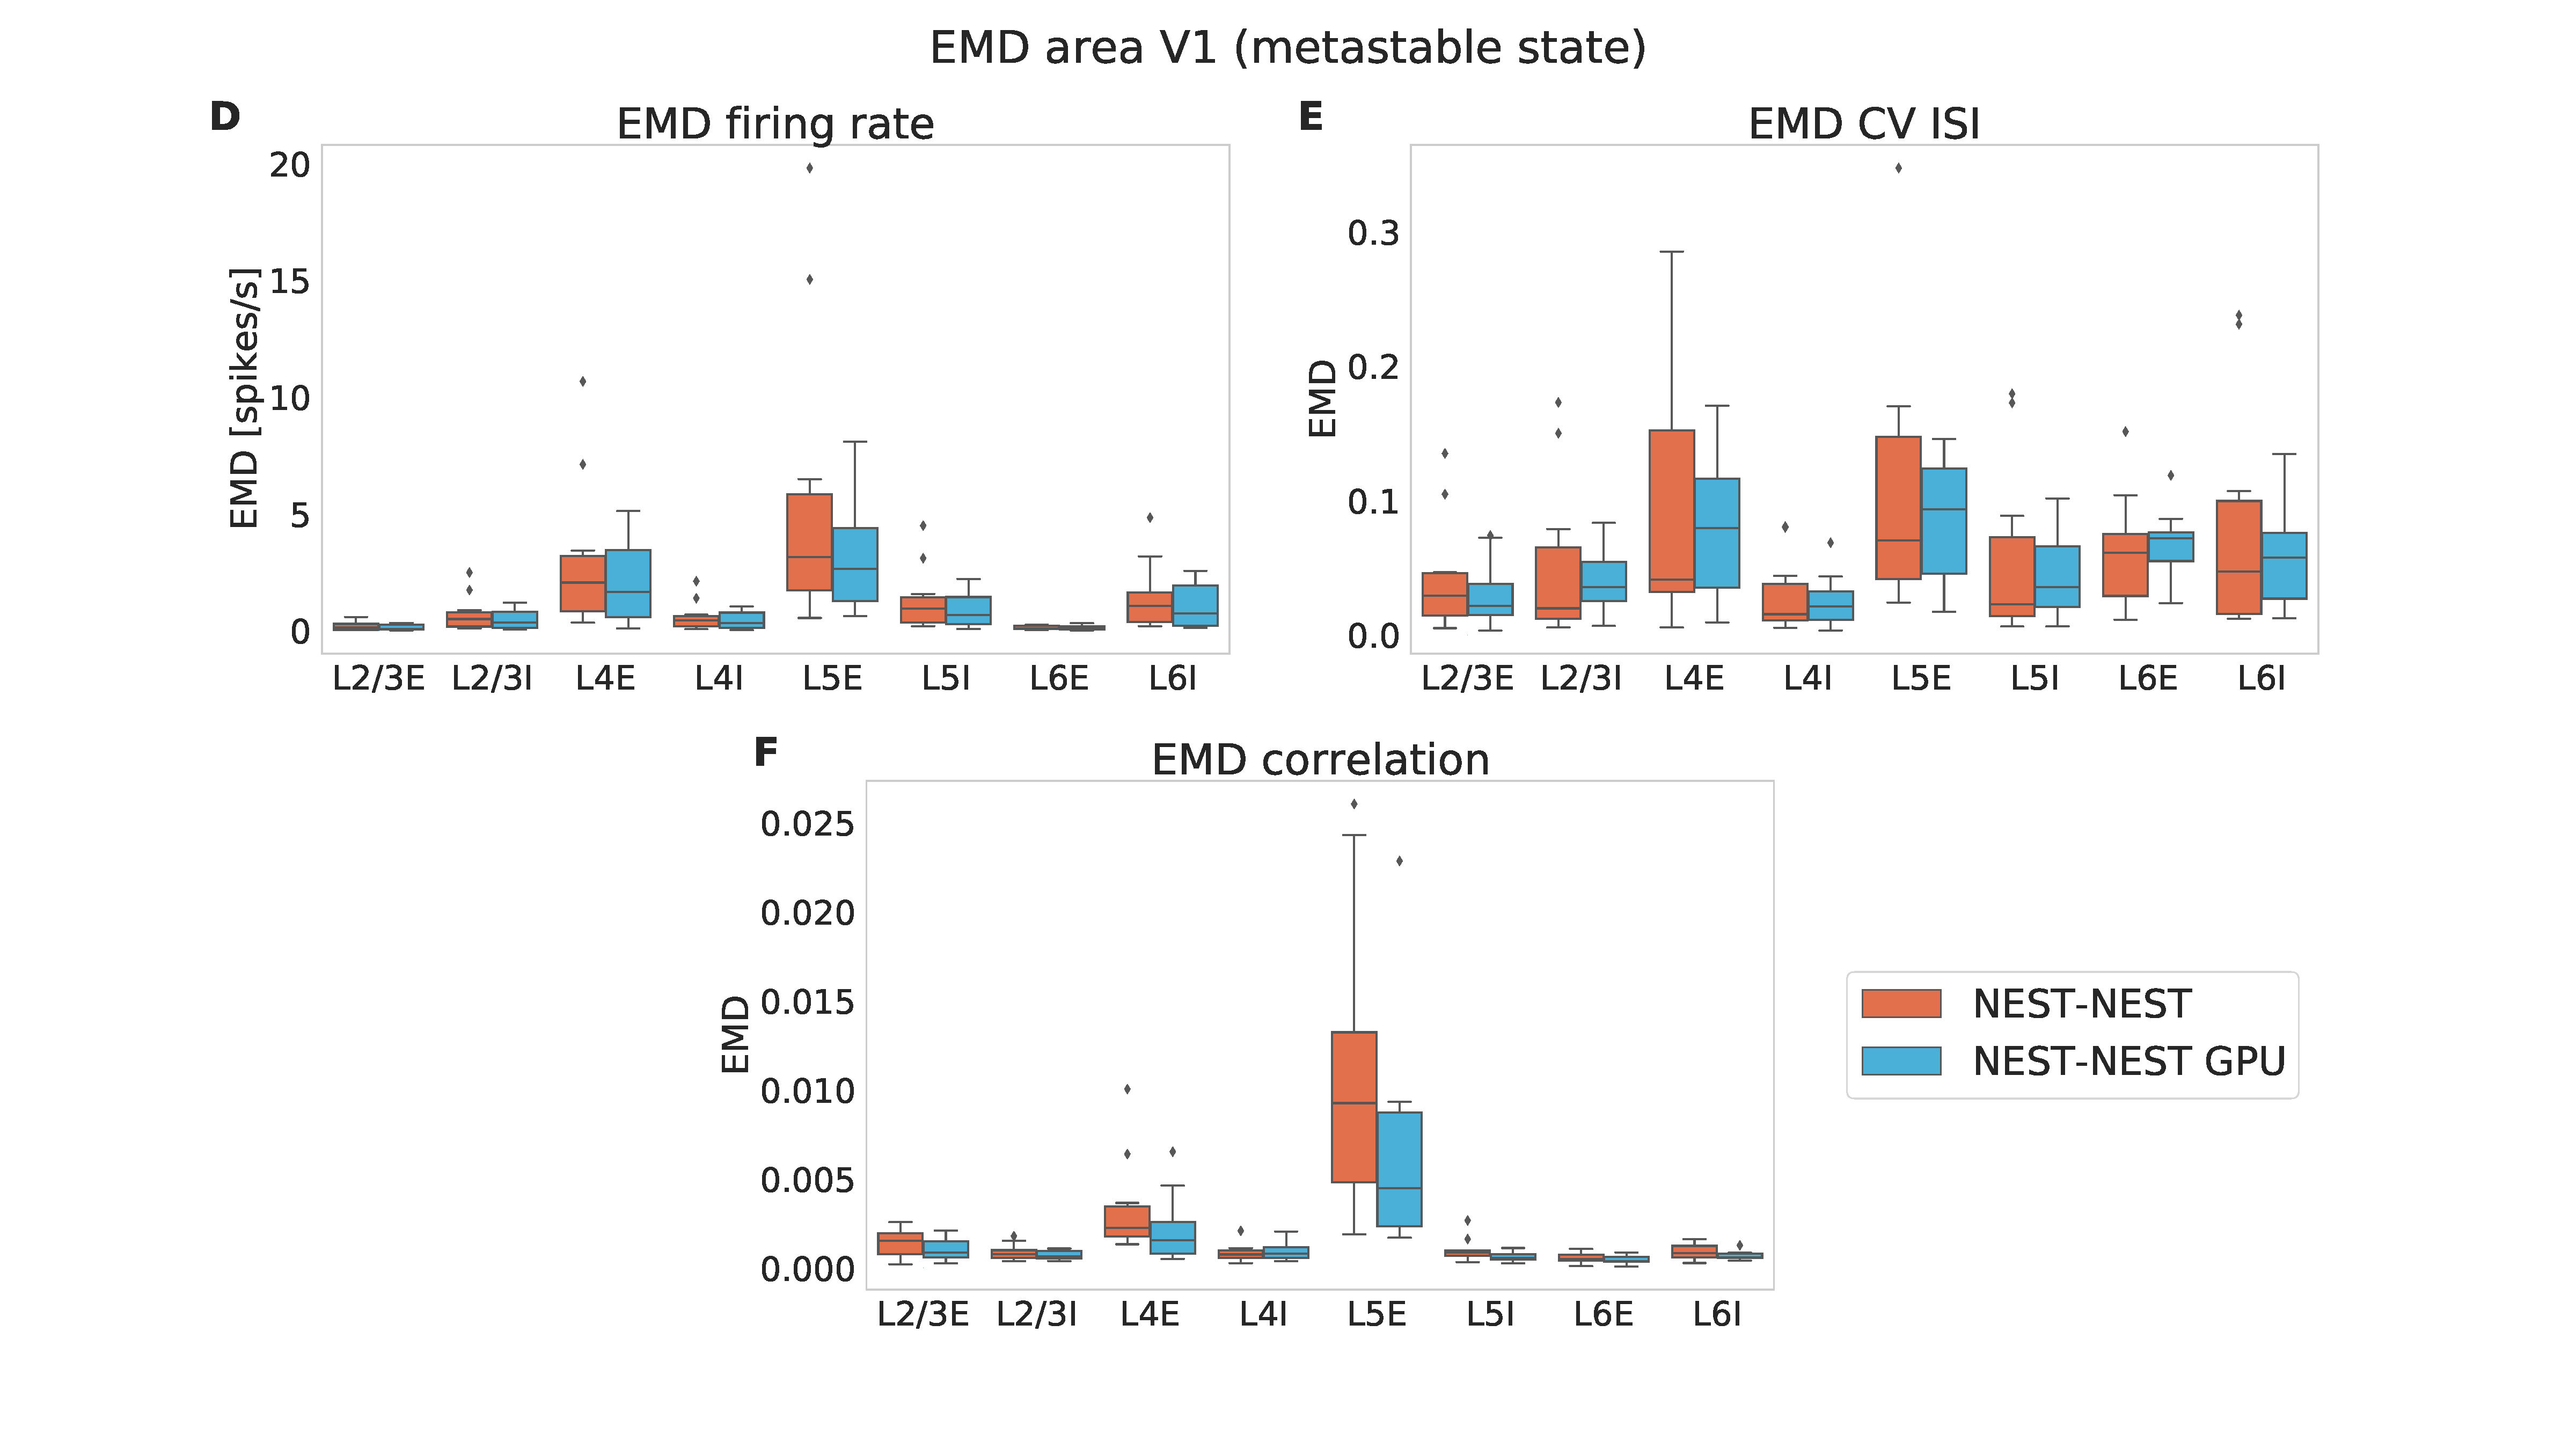
\includegraphics[trim=6cm 0 6cm 0, clip,width=\columnwidth]{figures/emd_boxplot_sample_ms.pdf}
    \caption{Earth Mover’s Distance between distributions of firing rate, CV ISI and correlation of the spike trains obtained from the area V1 of the model in the ground state \textbf{(A,B,C)} and the metastable state \textbf{(D,E,F)} simulated with NEST and NEST GPU. EMD boxes are obtained comparing NEST using different seeds (NEST-NEST, orange) and NEST and NEST GPU (NEST-NEST GPU, sky blue).}
    \label{fig:mam_sample_emd}
\end{figure}


Figure \ref{fig:mam_sample_emd} shows that the EMD values for the NEST-NEST GPU comparison are distributed similarly to those for the NEST-NEST comparison, meaning that the differences that arise due to the choice of simulator are statistically similar to those between NEST simulations with different random number generator seeds. Thus, using NEST GPU instead of NEST (with different random seeds) does not add variability compared to using different random seeds with the same simulator. As a reference, only the results for the area V1 of the model are shown in this figure, however, the EMD box plots for all the populations and areas of the model are shown in Appendix \ref{app:mam_validation}. This is a further indication that NEST and NEST GPU yield statistically closely similar results. EMD values obtained by the comparison of the ground state distributions are significantly smaller than the EMD values obtained for the metastable state. This is due to the increased fluctuations in the latter state of the model. In some cases, whiskers for the NEST-NEST and NEST-NEST GPU comparisons have different extents. This may be related to long-tailed distributions of the corresponding activity statistics. Indeed, differences in the tails of the distributions caused by only a few data points can lead to large differences in EMD values because the probability mass needs to be moved over large distances to turn one distribution into another. Moreover, each EMD box is only formed by $10$ values of EMD, since each set of simulations comprises $10$ simulations. Indeed, a larger amount of data would decrease the differences between the box plots shown, however, such a work would need a considerable amount of computed time which can be reduced by future hardware and developments of the library.




\chapter{\textbf{NEST GPU performance evaluation}}
\label{chapter:performance_evaluation}

\begin{tcolorbox}[colback=white,colframe=DarkRed,title=\textbf{Summary}]
Here, NEST GPU performance is evaluated using different hardware and parallel configurations. First of all, benchmarks on the simulation of the cortical microcircuit model are presented, with a focus both in the network construction and in the simulation of the network dynamics. Then, performance on the simulation of the multi-area model on a MPI-GPU cluster is discussed. Finally, the scaling performance of the simulator is shown using the balanced network model with a different number of neurons and synapses.\\
Benchmarks oriented towards the estimation of the network construction time on NEST GPU are performed by me and Jose Villamar, a PhD student at the Institute of Neuroscience and Medicine (INM-6) of the Jülich Research Center (Germany).
\end{tcolorbox}

\section{Phases of the simulation}
To properly evaluate the performance of the library we have to distinguish at least two phases of the overall simulation time (or time-to-solution): \textit{network construction} and \textit{simulation}. Network construction phase handles all the steps until the actual simulation of the network dynamics starts, with the latter handled by the simulation phase. To go more into the detail, network construction phase is characterized by the following stages:
\begin{itemize}
    \item \textit{initialization}, which is a setup phase in the Python script that import modules, sets the parameters, etc;
    \item \textit{node creation}, which instantiates the neurons and the devices of the network model;
    \item \textit{node connection}, which instantiates the connections between the network nodes;
    \item \textit{calibration}, a preparation phase in which connections are properly ordered and organized suitably for the spike delivery algorithm, and spike buffers and spike arrays are initialized.
\end{itemize}

In the previous version of NEST GPU and in the prototype library NeuronGPU, the calibration phase was also used to move the data from RAM to GPU memory, since the network construction phase was done at the CPU level and then copied to GPU. However, the novel algorithm proposed in \cite{Golosio2023} directly performs the network construction phase on the GPU device, avoiding the copy operation.\\
As the network construction phase, also the simulation phase can be divided in subtasks, which are:
\begin{itemize}
    \item \textit{delivery}, which represents the time for local spike handling and delivery;
    \item \textit{communication}, which describes the time for remote (i.e., trough MPI) spike handling and delivery. This subtask is present only for multi-GPU simulations;
    \item \textit{collocation}, which describes the time needed for preparing the MPI send buffers (ergo is present only in multi-GPU simulations);
    \item \textit{update}, representing the time needed to update the dynamics of neurons and synapses;
    \item \textit{other}, which is a general subtask that collects minor contributions to the simulation time that do not belong to the previous subtasks.
\end{itemize}


\section{Simulations of the cortical microcircuit model}
After having validated NEST GPU on the simulation of the cortical microcircuit model in Section \ref{sec:cm_validation}, here we evaluate the performance of the library. Simulations of such a network model are usually performed on a single GPU since the full scale model easily fits the GPU memory of relatively recent GPU cards, and even high-end laptops can simulate the model within a reasonable time-to-solution.\\
Here we divide the performance evaluation on the simulation of the cortical microcircuit into two subsections to distinguish between the performance evaluation of the network construction phase and the simulation of the network dynamics.

\subsection{Network construction time performance}
Network construction phase is an "intensive property" of the overall simulation, meaning that it does not depend on the biological time we want to simulate. Thus, an appropriate time for simulating the dynamics would lead to a minor contribution of this time to the overall simulation time. However, it should not be considered as a simple overhead not worthy to be optimized. Indeed, this phase can have a significant time contribution in certain applications such as parameter scans, in which several simulations are needed to be tested and thus a non-optimized network construction phase would strongly condition the overall time.\\
In \cite{Golosio2023} we tested the new network construction algorithm able to construct the network at runtime on GPU. We validated the new algorithm, which currently can only be applied to single-GPU simulations, on the simulation of the cortical microcircuit model. While in the previous version of NEST GPU the network construction depended on the CPU of the workstation, now this time depends uniquely on the GPU card employed (as the simulation time).\\
To evaluate the performance on this stage, we used different systems employing different NVIDIA GPU cards. The table below fully describes the hardware these systems are equipped with.

\begin{table}[H]
\centering
\resizebox{\columnwidth}{!}{%
\begin{tabular}{|>{\centering\arraybackslash}p{0.2\linewidth}|>{\centering\arraybackslash}p{0.4\linewidth}|>{\centering\arraybackslash}p{0.4\linewidth}|}
\hline
\rowcolor[HTML]{333333} 
\multicolumn{1}{|c|}{\cellcolor[HTML]{333333}{\color[HTML]{FFFFFF} \textbf{System}}} & \multicolumn{1}{c|}{\cellcolor[HTML]{333333}{\color[HTML]{FFFFFF} \textbf{CPU}}} & \multicolumn{1}{c|}{\cellcolor[HTML]{333333}{\color[HTML]{FFFFFF} \textbf{GPU}}} \\ \hline
JUSUF cluster (node) & 2$\times$ AMD EPYC 7742, $2\times 64$ cores, 2.25 GHz & NVIDIA V100, 1530 MHz, 16 GB HBM2e, 5120 CUDA cores \\ \hline
JURECA-DC cluster (node) & 2$\times$ AMD EPYC 7742, $2\times 64$ cores, 2.25 GHz & NVIDIA A100, 1410 MHz, 40 GB HBM2e, 6912 CUDA cores \\ \hline
Workstation 1 & Intel Core i9-9900K, 8 cores, 3.60 GHz & NVIDIA RTX 2080 Ti, 1545 MHz, 11 GB GDDR6, 4352 CUDA cores \\ \hline
Workstation 2 & Intel Core i9-10940X, 14 cores, 3.30 GHz & NVIDIA RTX 4090, 2520 MHz, 24 GB GDDR6X, 16384 CUDA cores \\ \hline
\end{tabular}}
\caption{Hardware configuration of the different systems used to evaluate the performances. Cluster information is given on a per node basis.}
\label{tab:workstations}
\end{table}

First of all, we want to compare the performance of the new algorithm of network construction of NEST GPU with the previous one. We call \textit{NEST GPU onboard} the version of NEST GPU which implements the novel algorithm, since all the phases of the simulation take place on the GPU card. We call then \textit{NEST GPU offboard} the previous version of the library for which the network construction phase was handled by the CPU and then the network was copied in the GPU memory for the simulation of the network dynamics.\\
For the comparison, we performed $10$ simulations using different seeds for every system configuration shown in Table \ref{tab:workstations}. Times are extracted using Python timers, in particular using the function \texttt{perf\_counter\_ns} of the \texttt{time} module, which returns each time measured in nanoseconds, i.e., the best possible resolution at Python level.\\
Figure \ref{fig:cm_network_construction_ngpu} directly compares the two network construction approaches using the different computing systems described in Table \ref{tab:workstations}.

\begin{figure}[H]
    \centering
    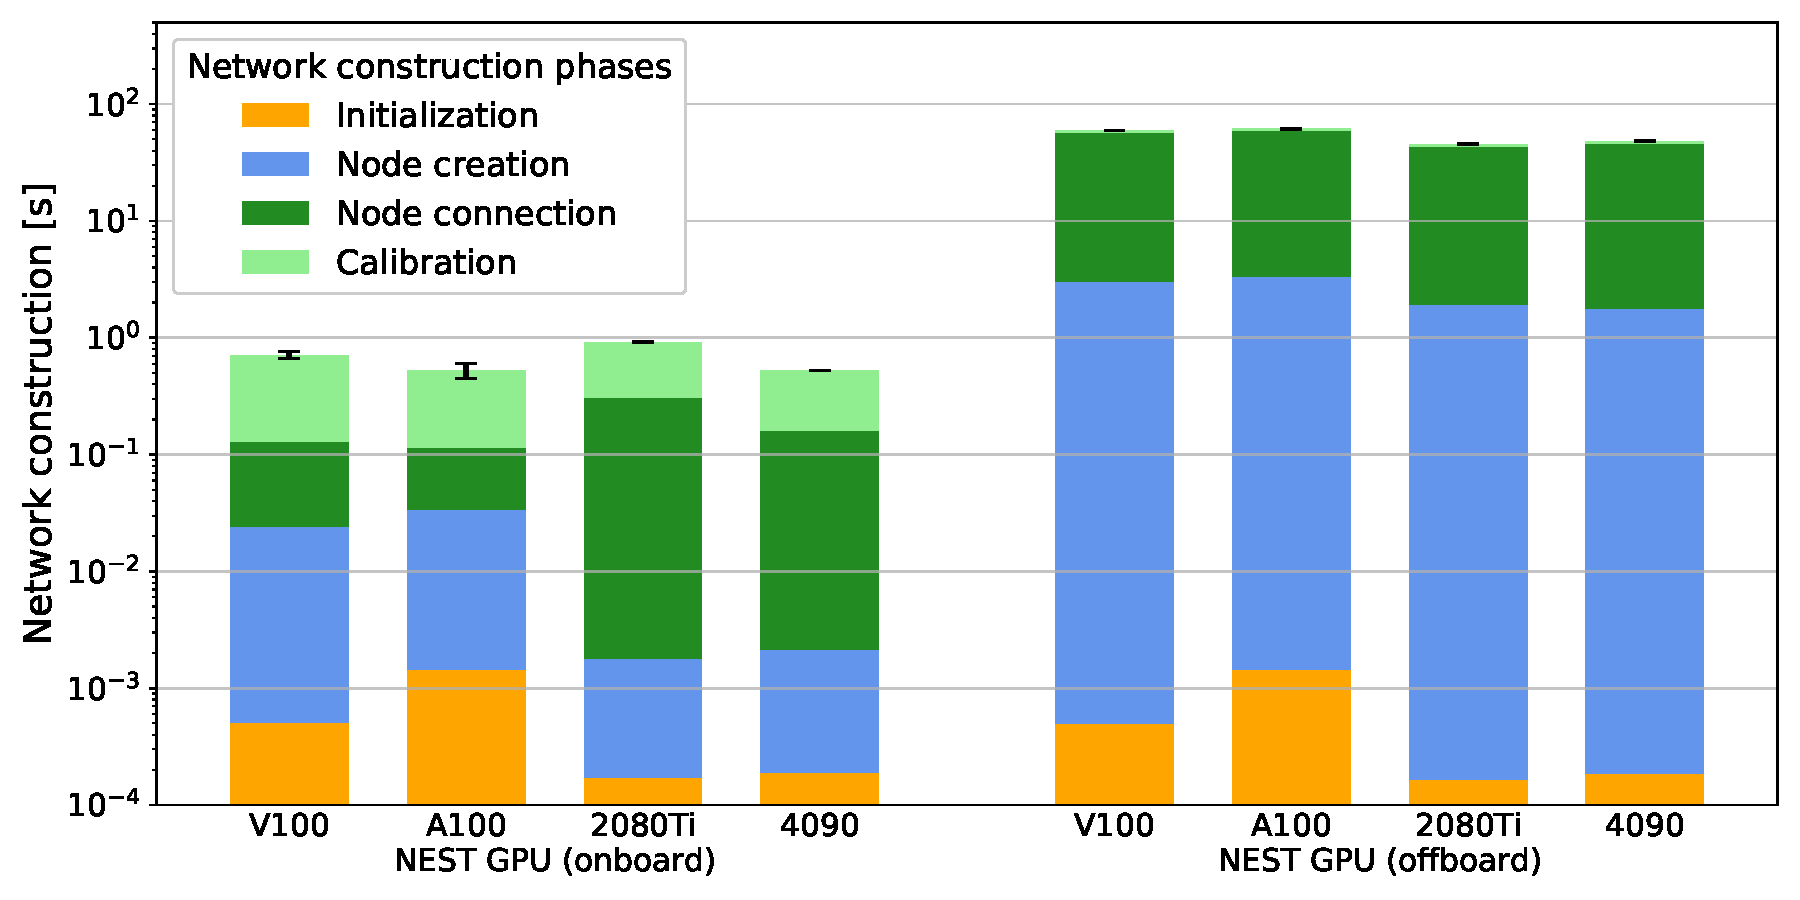
\includegraphics[width=\columnwidth]{figures/cm_ngpu_net_constr.pdf}
    \caption{Comparison of network construction phase for the two versions of NEST GPU in the simulation of the cortical microcircuit model. Simulations are performed on different hardware configurations, here indicated with the GPU device they equip. Error bars show the standard deviation of the time needed for network construction over ten simulations using different seeds. Figure adapted from \cite{Golosio2023}.}
    \label{fig:cm_network_construction_ngpu}
\end{figure}

As can be seen, the novel method for network construction directly on GPU memory outperforms the method applied in the previous version of the library, granting a speed-up of two order of magnitude. With this method, the full-scale cortical microcircuit model can be simulated in less than a second both on consumer-grade GPUs and data center GPUs.\\
Additionally, we also compared the performance of the novel algorithm with the CPU-based simulator NEST (version 3.3 \cite{nest3.3}) and the GPU-based GeNN \cite{Yavuz2016} (version 4.8.0\footnote{\url{https://github.com/genn-team/genn/releases/tag/4.8.0}}). In particular, the GeNN simulator differs in terms of network construction approach to NEST GPU since it adopts a code-generation approach. Thus, GeNN code has to be generated and compiled before execution. In this simulator the network construction phase can be decomposed in the following subtasks:
\begin{itemize}
    \item \textit{model definition}, which defines neurons, devices and synapses of the network;
    \item \textit{building}, which generates and compiles the simulation code;
    \item \textit{loading}, which allocates memory and instantiate the network on the GPU.
\end{itemize}
Also in this case, the time to complete the subtasks is measured through Python timers. Regarding NEST, the network construction is done at runtime as in NEST GPU, with analogous network construction subtasks. Figure \ref{fig:network_construction_ngpu_nest_genn} shows the network construction time for NEST GPU, NEST and GeNN using different hardware configurations.

\begin{figure}
    \centering
    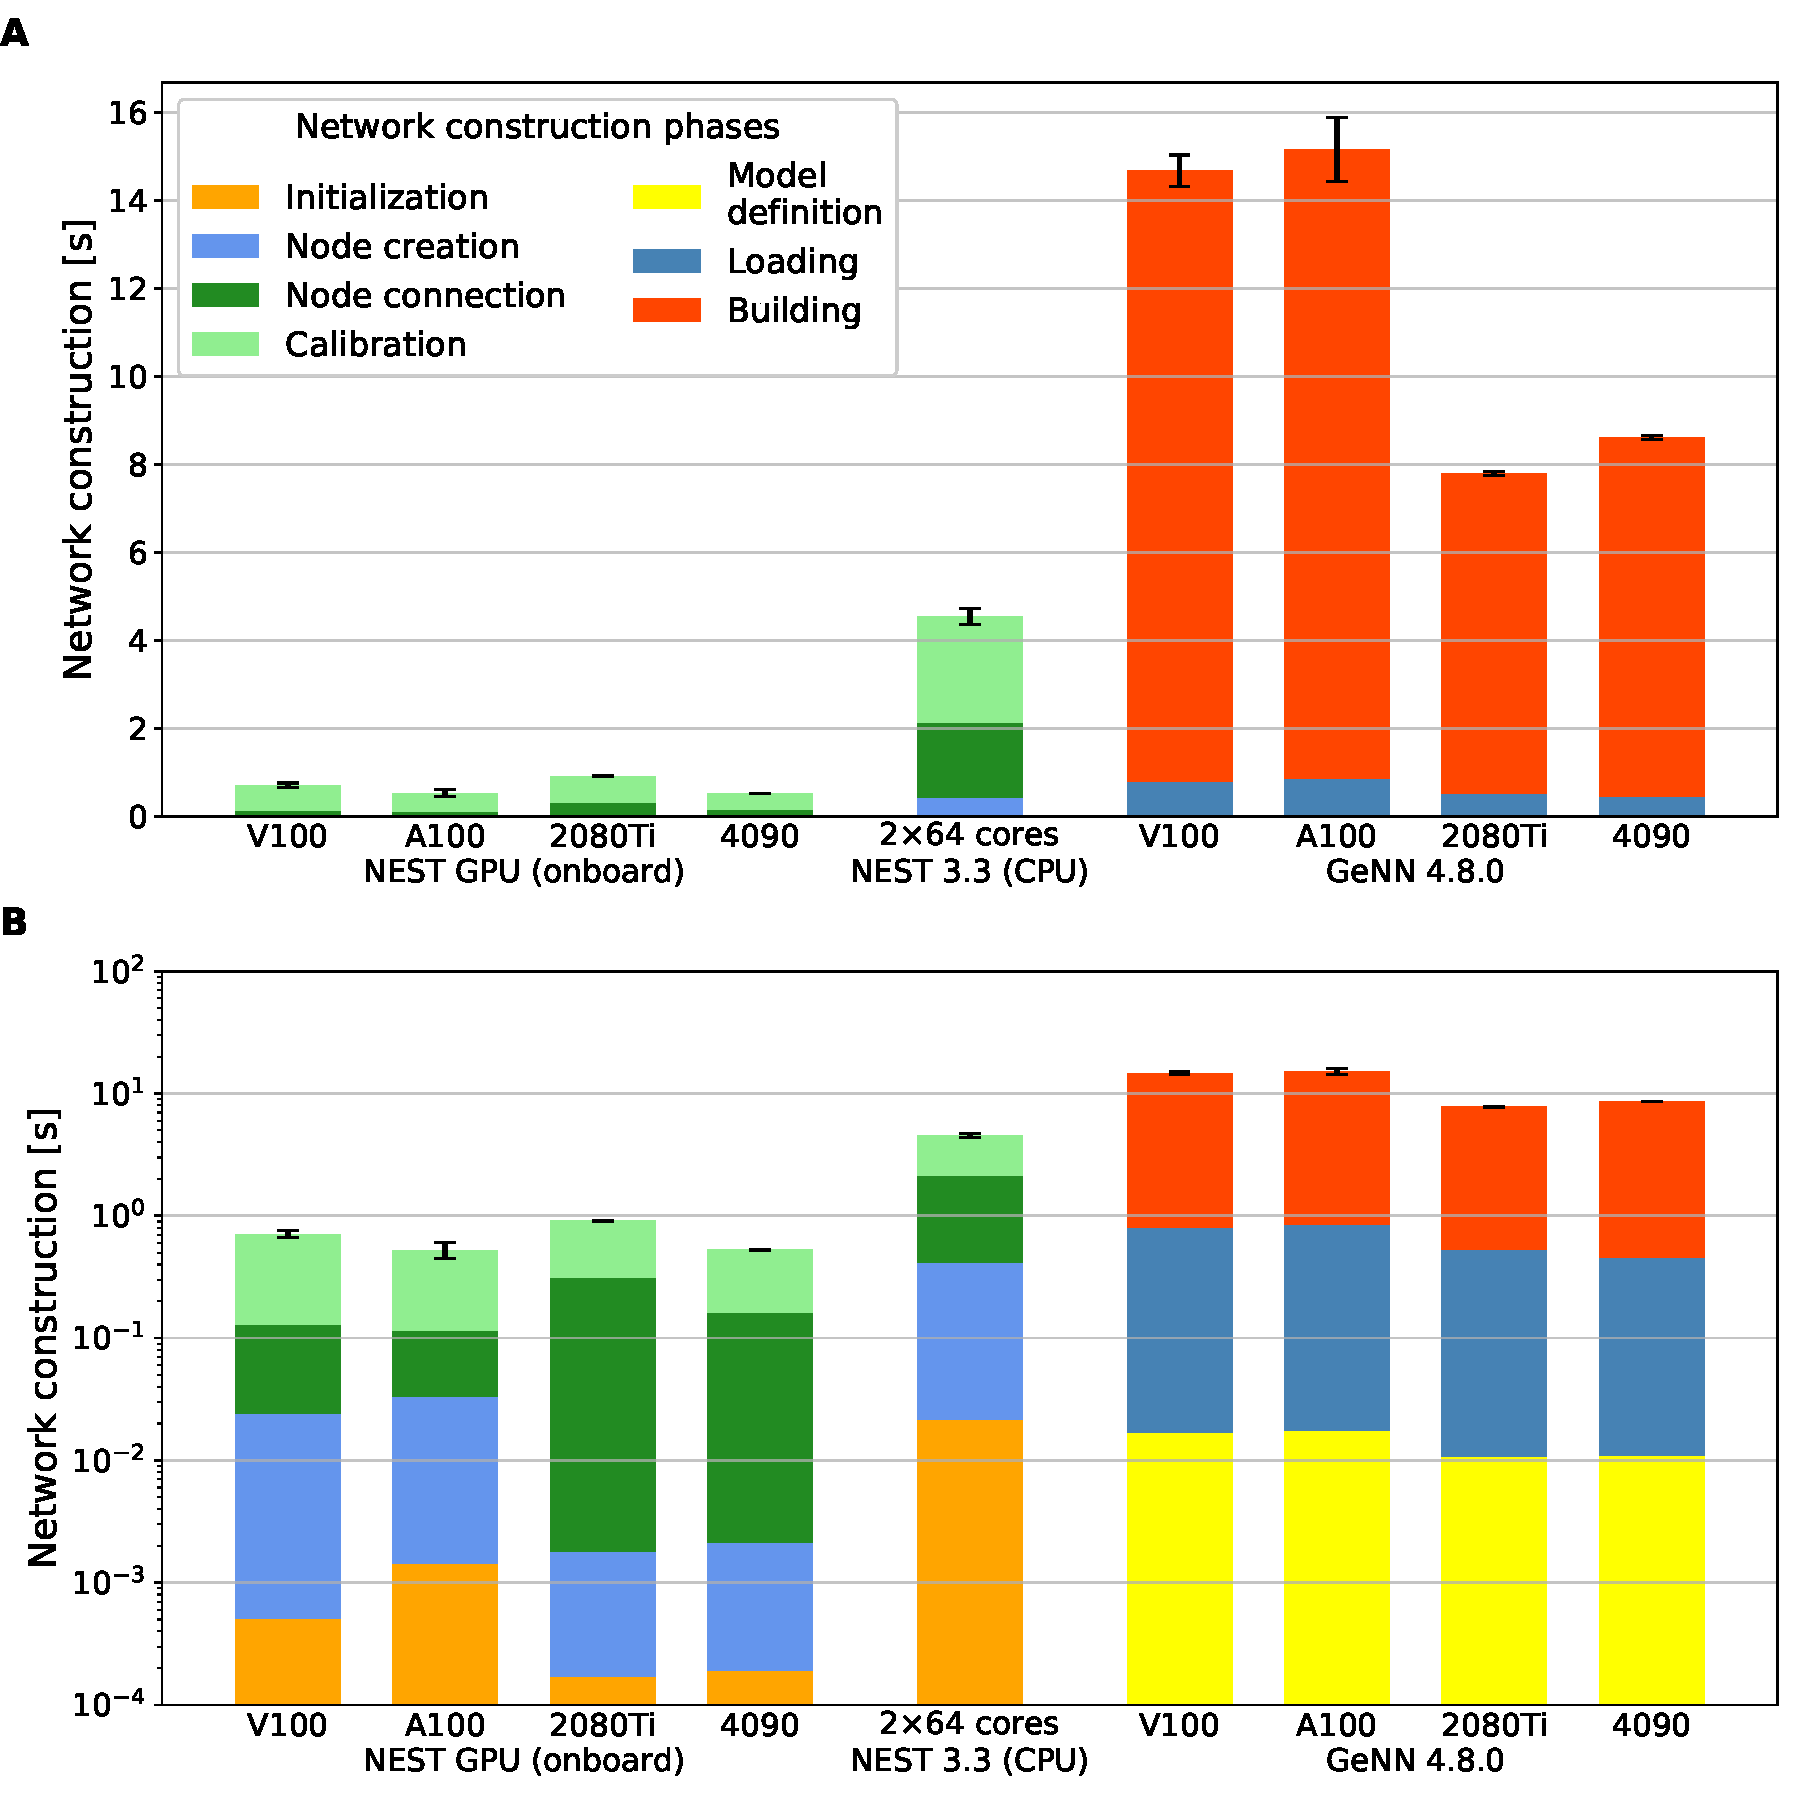
\includegraphics[width=\columnwidth]{figures/cm_net_constr.pdf}
    \caption{Performance comparison of the network construction phase for different simulators and hardware configurations on the cortical microcircuit model. Data for NEST GPU \textit{(onboard)} is the same as in Figure \ref{fig:cm_network_construction_ngpu}.
    \textbf{(A)}~Network construction time of the model in linear scale for different simulators and hardware configurations.
    \textbf{(B)}~as in \textbf{A}~but with logarithmic y-axis scale.
    In both panels, the \textit{building} phase of GeNN is placed on top of the bar, breaking with the otherwise chronological order, because this phase is not always required and at the same time, this display makes the shorter \textit{loading} phase visible in the plot with the logarithmic y-axis.
    Error bars show the standard deviation of the overall network construction phase over ten simulations using different random seeds. Figure from \cite{Golosio2023}.}
    \label{fig:network_construction_ngpu_nest_genn}
\end{figure}

As can be noticed, NEST GPU results faster in the network construction with respect to NEST, and also to GeNN. However, it should be noted that the \textit{building} phase of GeNN, related to code creation and compilation, take place only if code has not been generated and compiled or when network parameters have to be changed. If these are not the cases, this phase is not present, making the network construction times of NEST GPU and GeNN totally compatible. Nonetheless, NEST GPU approach works on runtime, so the time for code compilation is not needed anyway, increasing the flexibility of this phase.\\
Moreover, Figure \ref{fig:network_construction_ngpu_nest_genn} shows the performance for network construction when, in NEST and NEST GPU, external stimulation of the model is driven by Poisson spikes generators. Indeed, the NEST and NEST GPU implementations can have this kind of device or DC input as external stimulation. However, the network construction times obtained using the DC input in NEST and NEST GPU are totally similar to the one shown in the figure.\\
In summary, the new network construction of NEST GPU is able to achieve state-of-the art performance in the network construction of networks that can be simulated on single GPUs. Indeed, NEST GPU network construction times are compatible with code generation-based simulation codes such as GeNN. Currently, the major limitation of this algorithm is that it can be employed only for single-GPU simulations, however, an extension for the algorithm to multi-GPU simulations is in development. A discussion about the idea behind this extension of the algorithm and how should it work is presented in the outlook of this thesis.

\subsection{Simulation performance}
Evaluating the simulation performance is important to provide an efficient simulation code: indeed, codes that run at realtime are fundamental for several applications, such as robotics and studies of large-scale models oriented towards the study of cognitive processes and brain development in general. As a normal practice, when evaluating simulation performance spike recording is disabled. Differently from the network construction phase, the simulation phase is an "extensive measure", meaning that the lenght of the wall-clock time depends on the amount of biological time that has to be simulated. In order to provide a measure to assess the simulation speed we use the real-time factor (RTF), defined as
\begin{equation}
\label{eq:RTF}
    \text{RTF} = \dfrac{T_{\text{wall}}}{T_{\text{model}}}
\end{equation}
where $T_{\text{wall}}$ is the wall-clock time, i.e., the time needed for the simulator to complete the simulation of the network dynamics, whereas $T_{\text{model}}$ is the biological time that is simulated.\\
Here we evaluate the performance of the simulation of the network dynamics for NEST GPU (onboard) on the simulation of the cortical microcircuit model. To simplify the notation, from now on we will drop the term "onboard" so that for NEST GPU we refer to the most recent version of the library.\\
Since this model was the most tested one when optimizing the library, here we can provide benchmarks using different versions of the library. In particular, we will focus on the simulation of the model using the Poisson signal generators as external stimulation. Indeed, there is a relevant difference in the simulation time when Poisson signals or DC input are employed for external stimulation, with the latter leading to the best performance. However, since a stimulation through Poisson-like spike trains is the most plausible from a neuroscientific point of view, the plot, if not specified, will show the performance when these devices are employed on NEST and NEST GPU simulations.\\
To show the improvement of the library over the last few years, Figure \ref{fig:nest_nestgpu_RTF} shows the simulation time of the current version of NEST GPU and the prototype library NeuronGPU using the different hardware systems shown in Table \ref{tab:workstations}.

\begin{figure}[H]
    \centering
    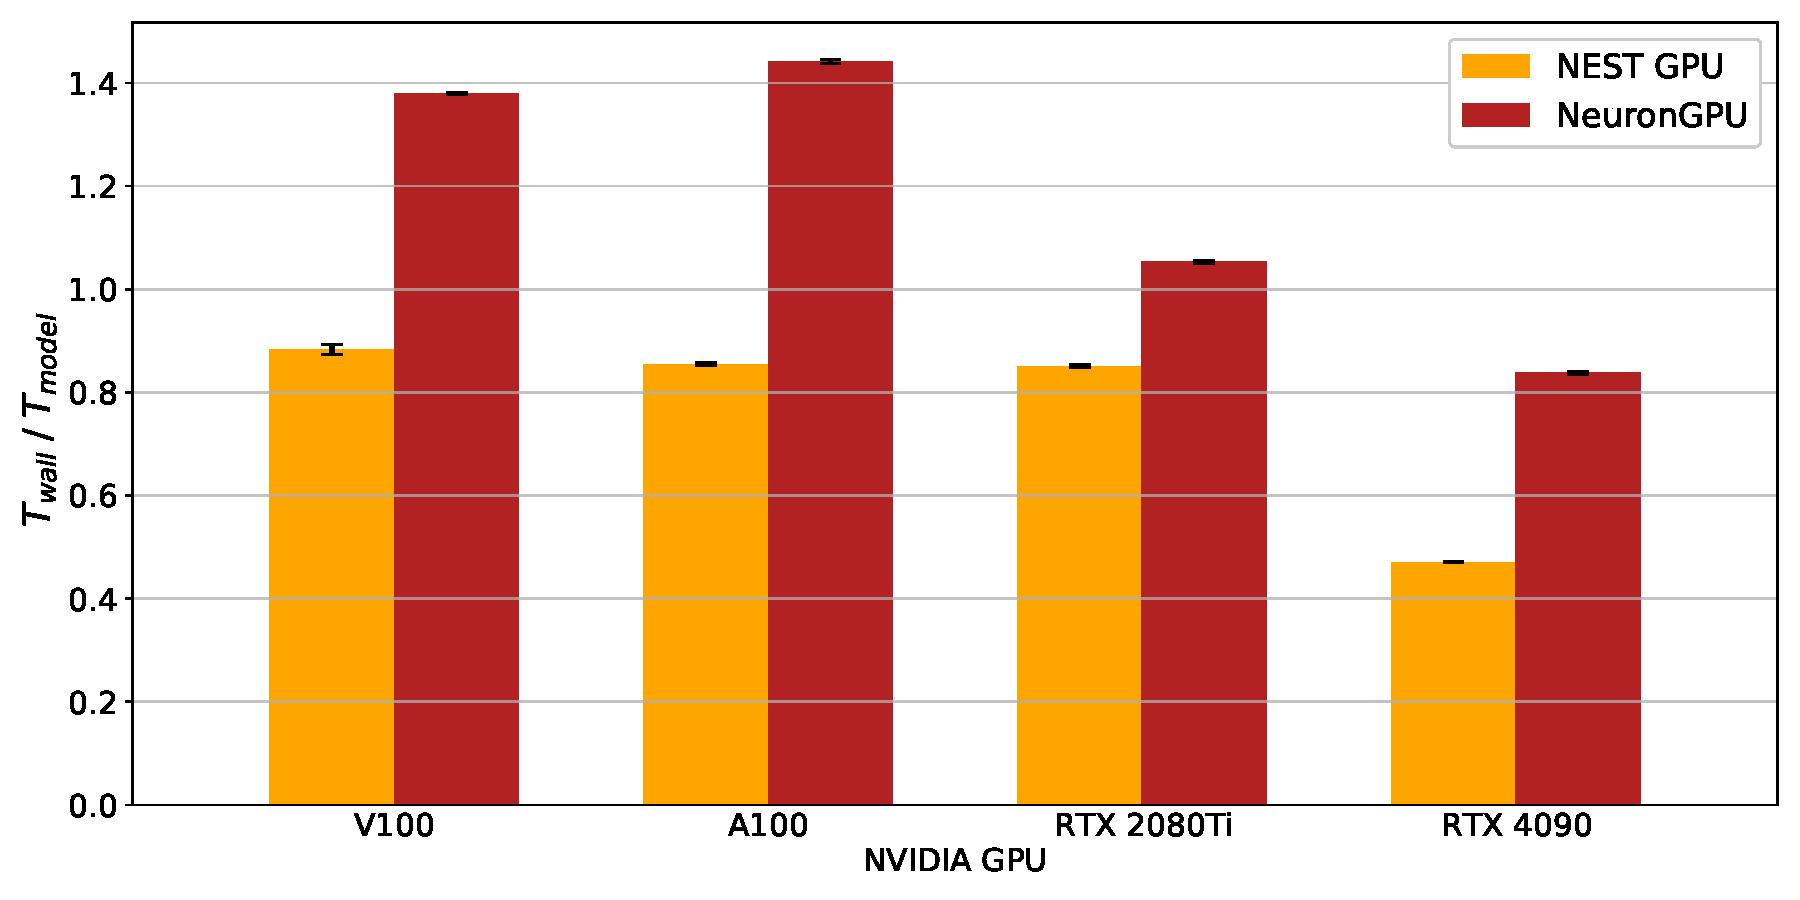
\includegraphics[width=\columnwidth]{figures/cm_nestgpu_neurongpu_RTF.pdf}
    \caption{Real-time factor of cortical circuit model simulations for NEST GPU (amber) and NeuronGPU (dark red). Here, $T_{\text{model}}=10$\,s and $10$ simulations for each hardware configuration are performed. Error bars show the standard deviation calculated over the $10$ simulations.}
    \label{fig:nest_nestgpu_RTF}
\end{figure}

As can be seen, NEST GPU library as been optimized in the simulation phase, with improvements that spans from $55\%$ to $75\%$ with respect to NeuronGPU, the prototype library introduced in \cite{Golosio2021}. This improvement is mainly due to an optimization of the CUDA synchronous calls in the NEST GPU code, which were removed when unnecessary. This led to a removal of the latency due to the synchronization between CUDA threads during the simulation phase which were not necessary for performing simulations correctly. This work was done with the help of NVIDIA developers in the context of a GPU hackathon, during which me and the rest of the NEST GPU team were involved in several optimizations of the GPU code of the library. In that context we also focused on the implementation of multiple algorithms to perform nested loops on GPU code in the most efficient way possible. Indeed, part of the performance improvement is also due to the choice of a more efficient algorithm for this operation. In this regard, further work is needed to evaluate the most efficient algorithm to perform this task and, more in general, optimization of the library using techniques such as performance profiling will be object of future work to further improve NEST GPU performance. This topic will be discussed in the outlook of this thesis.\\
Together with the comparison of the results of the spiking activity, we also compare the performance of NEST and NEST GPU. Moreover, we also perform comparison between NEST GPU and other GPU-based simulators such as GeNN \cite{Yavuz2016}, which has established itself as one of the most used GPU-based simulation codes. In particular, in \cite{Knight2018} it was presented the GeNN implementation of the cortical microcircuit model, thus we decided to compare the two simulators in the simulation of this model. Indeed, results changed over the last years: next figure shows the results of the comparison obtained in \cite{Golosio2021} and the one obtained in \cite{Golosio2023} for different versions of the GPU libraries.

\begin{figure}[H]
    \centering
    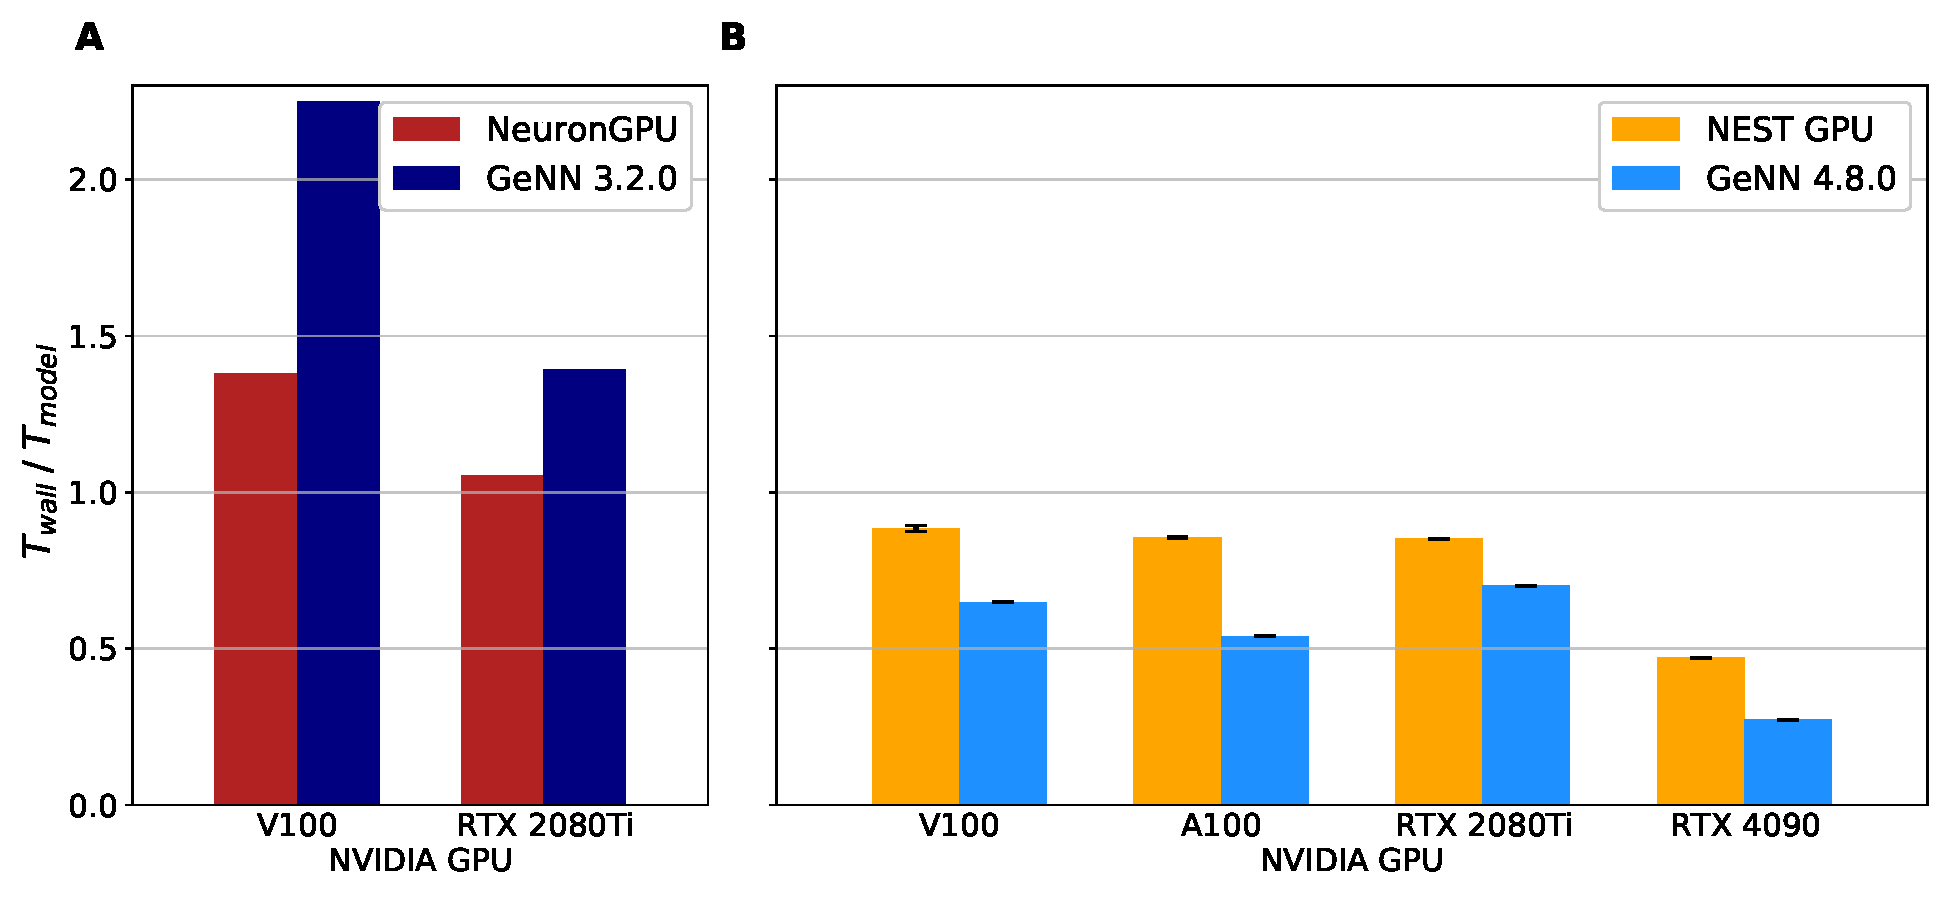
\includegraphics[width=\columnwidth]{figures/cm_RTF_old_new.pdf}
    \caption{Real-time factor using different NVIDIA GPUs for different GPU-based simulation codes. \textbf{(A)} real-time factor of the prototype library NeuronGPU (red) and GeNN 3.2.0 (navy), from \cite{Golosio2021}. \textbf{(B)} real-time factor of the most recent version of NEST GPU (amber) and GeNN 4.8.0 (sky blue). Data for NEST GPU is the same of Figure \ref{fig:nest_nestgpu_RTF}.}
    \label{fig:cm_rtf_old_new}
\end{figure}

As can be seen, panel A shows that, using the same GPU hardware, NeuronGPU was able to outperform GeNN (version 3.2.0 \footnote{\url{https://github.com/genn-team/genn/releases/tag/3.2.0}}), whereas in the current version of the libraries (see panel B), GeNN performs the simulation of the cortical microcircuit faster than NEST GPU.\\
However, simulations on NEST GPU here uses Poisson signal generator as external input. Indeed, the usage of DC input can lead to a remarkable speed-up of the simulation. GeNN employs a different mechanisms for external stimulation, which mimics incoming Poisson spike trains through a current directly applied to each neuron. For this reason, it is interesting to compare both the NEST GPU implementations with Poisson spike and the DC input-driven stimulation with the GeNN code.\\
To represent the current state-of-art for the simulation of the cortical microcircuit model on conventional computing architectures, next figure represents the real-time factor for NEST GPU, GeNN 4.8.0 and NEST. The NEST (GPU and CPU) performance is measured both when employing the Poisson spike generators and DC inputs as external stimulation.

\begin{figure}[H]
    \centering
    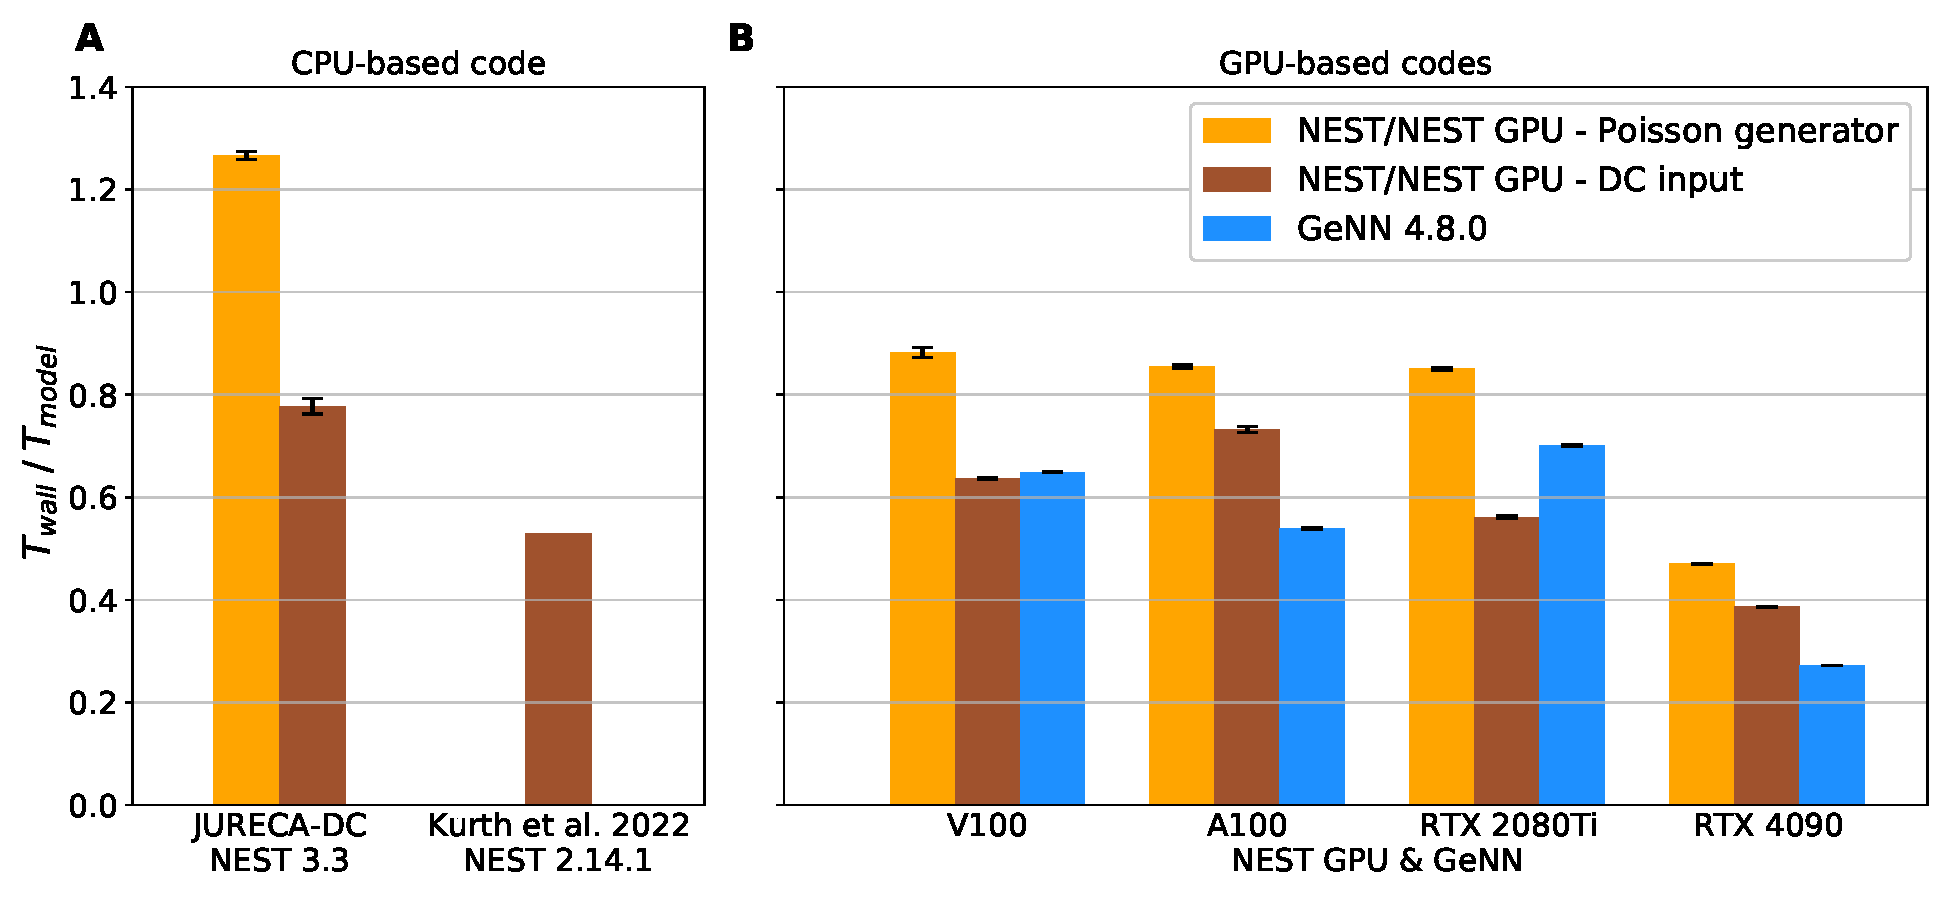
\includegraphics[width=\columnwidth]{figures/cm_overall_real_time_fact.pdf}
    \caption{Real-time factor using different CPU-based and GPU-based simulation codes, with the model employing different external stimuli; i.e., Poisson spike trains (amber), DC input (sienna) or the one designed by GeNN (sky blue). \textbf{(A)} real-time factor of different versions of NEST using different hardware and parallelization approaches. Data for NEST 3.3 from \cite{Golosio2023}, data for NEST 2.14.1 from \cite{Kurth2022}. \textbf{(B)} real-time factor of NEST GPU and GeNN 4.8.0 using different NVIDIA GPUs. Data from \cite{Golosio2023}.}
    \label{fig:cm_overall_RTF}
\end{figure}

To provide more detail on the NEST performance, the one of NEST 3.3 is presented on \cite{Golosio2023} and uses a single compute node of the HPC cluster JURECA-DC \cite{JURECA} (see also Table \ref{tab:workstations}), exploiting its 128 cores by 8 MPI processes each running 16 threads. The performance achieved using NEST 2.14.1 \cite{nest2.14.1} is from \cite{Kurth2022} and is obtained using two nodes equipped with two AMD EPYC Rome 7702 with $64$ cores each, with $2$ MPI processes per node. This result is, at the time of writing, the best result achieved by NEST in the simulation of this model.\\
Figure \ref{fig:cm_overall_RTF} shows that GPU-based performance are all below real time, with the best results achieved by GeNN or by NEST GPU when the external stimulation is driven by a DC input. It is also interesting to note that data center GPUs such as the NVIDIA V100 and the NVIDIA A100 shows performance compatible (or even slower) with respect to recent consumer GPUs such as the RTX 2080Ti and the RTX 4090. In particular, the remarkable results on the latter can be related to the higher clock speed of this GPU card. A further investigation of the relation between the performance and the specifications of the GPU device will be object of future work.

\section{Simulations of the multi-area model}
Here we present the performance evaluation of the multi-area model implementation for NEST GPU.
The network is comprised by 32 areas, each one designed similarly to the cortical microcircuit. NEST GPU simulations were performed using the JUSUF computing cluster \cite{JUSUF}, whereas NEST simulations were done on JURECA-DC \cite{JURECA}. See Table \ref{tab:workstations} for the specifications of each node of these computing clusters.\\
Since at most one of the model areas can be simulated on a single NVIDIA V100 (i.e., the GPU card with which JUSUF nodes are equipped), we decided to parallelize the simulation as follows: we employ 32 nodes equipped with a GPU each, with a single MPI process per node. In this regard, we decided to simulate the model so that each area is simulated in a single MPI process, i.e. in a single GPU card.\\
Such an approach is possible thanks to the locality exploitation of NEST GPU, which enables the creation of entire neuron populations in a defined MPI process. Indeed, this is one of the major differences with respect to NEST, since the CPU code adopts a round-robin approach to evenly distribute the neurons across all the MPI processes. Indeed, this approach, adopted also in \cite{Pastorelli2019}, can be significantly advantageous for multi-area models such as the one simulated here, since the density of inter-area connections greatly exceed the density of intra-area connections. From a simulation point of view, this means that simulating each area in the same MPI process can greatly reduce the number of spikes that have to be sent to other areas of the model, thus reducing the compute load of MPI communication, which typically incurs higher overhead compared to intra-node communication.\\
To evaluate the performance on the simulation of this model, we simulated the ground state and the metastable state, without recording the spikes. While we employed 32 compute nodes with 1 MPI process each for the NEST GPU simulations, we performed a strong scaling using a variable amount of compute nodes for the NEST (version 3.0 \cite{nest3.0}) simulations, finding that the fastest performance were achieved when simulating the model on 32 nodes of JURECA-DC, with 8 MPI processes per node and 16 threads per task. The strong scaling was done using the benchmarking framework beNNch \cite{Albers2022}.\\
Regarding the version of NEST GPU employed, as previously mention, the most recent version of NEST GPU can not be used since it employs the network construction algorithm to construct the network in GPU memory, which has not yet been implemented for multi-GPU simulations. Moreover, the version used here version still differs from the one previously called NEST GPU (\textit{offboard}), since it lacks of the optimization mentioned in the previous section regarding asynchronous calls. This has the disadvantage of increasing the simulation time, but has the advantage of providing the exact times for the simulation subtasks, which the current version is still not able to provide\footnote{A solution for this issue is currently object of study from me and the rest of the NEST GPU team.}. This way, we can also evaluate the amount of time taken by each stage of the simulation, which can be advantageous when comparing also different approaches for network simulation across different MPI processes.\\
Figure \ref{fig:mam_benchmark} shows the real-time factor for the simulation of the multi-area model using NEST and NEST GPU.

\begin{figure}[H]
    \centering
    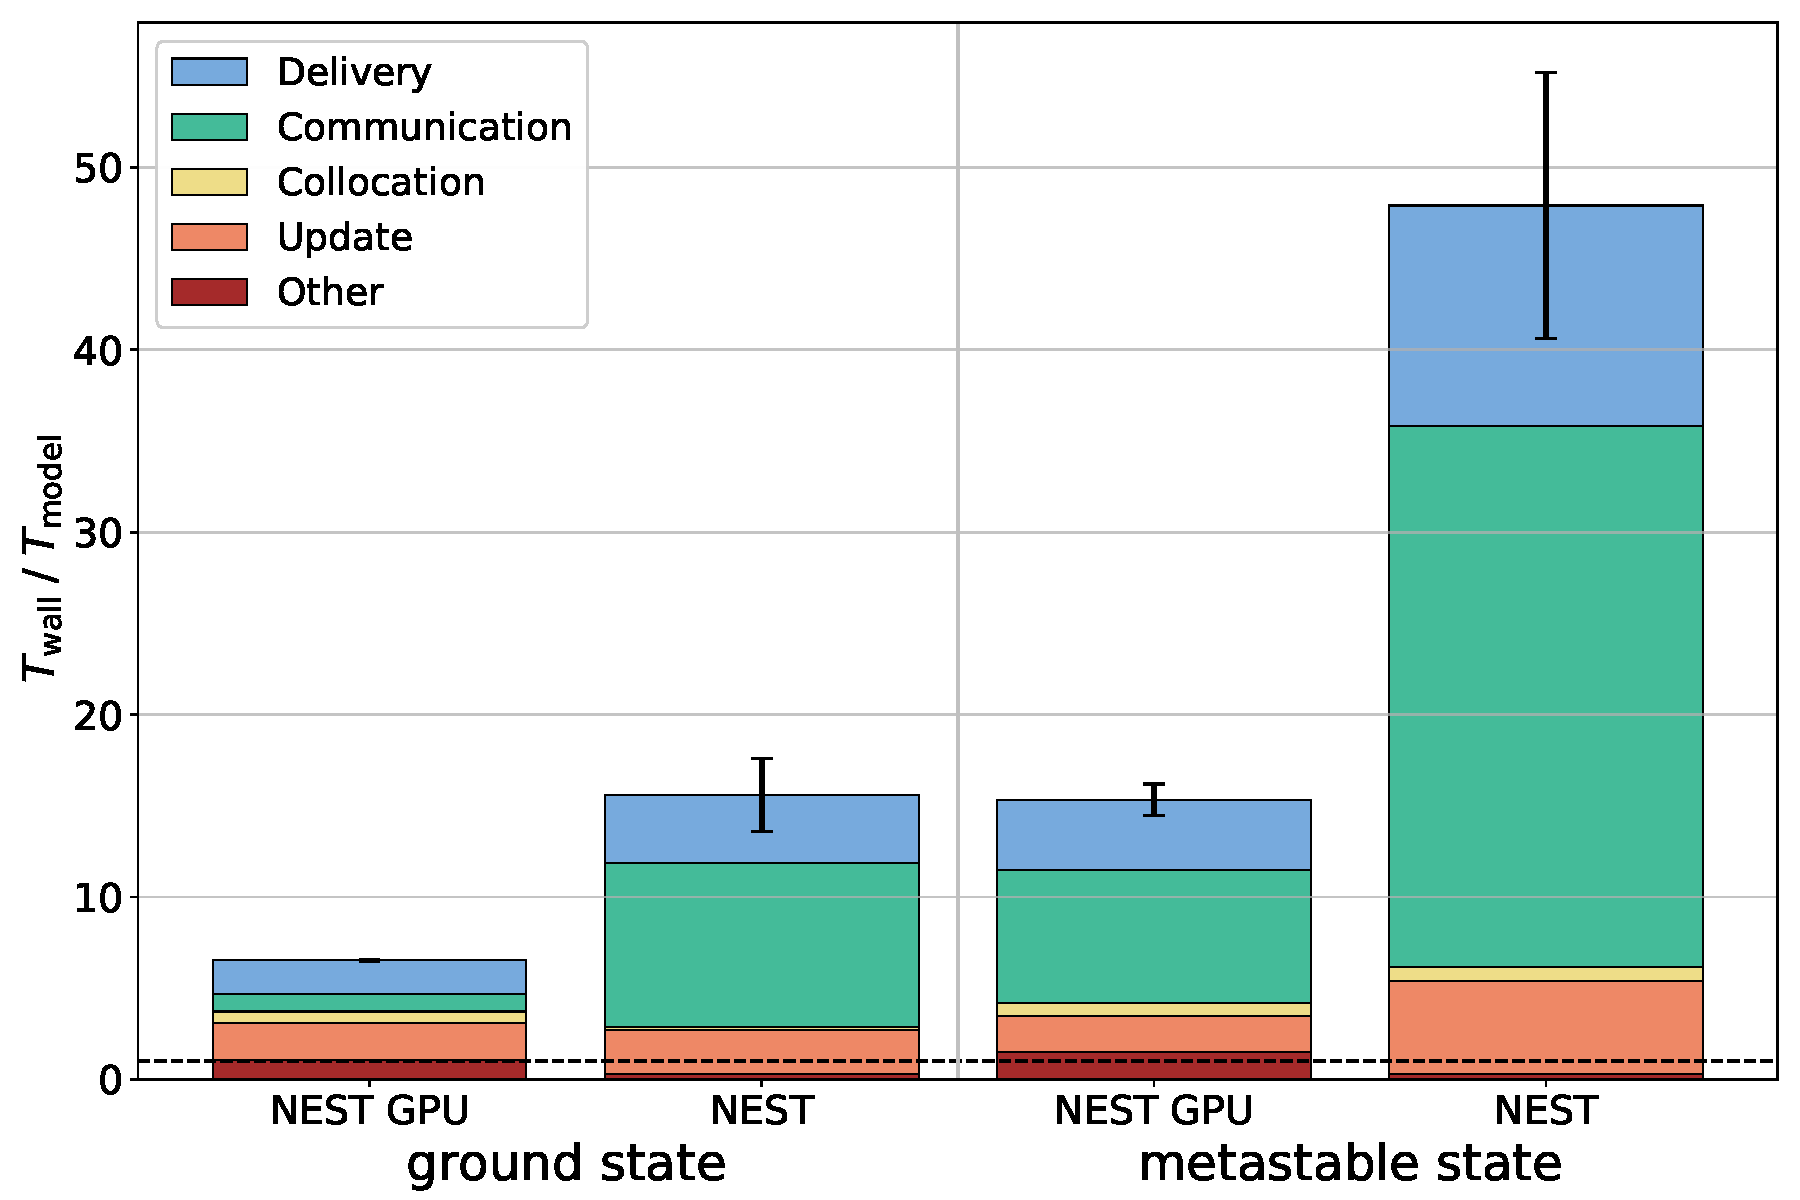
\includegraphics[width=\columnwidth]{figures/mam_rtf.pdf}
    \caption{Real-time factor for ground and metastable state simulations of the multi-area model using NEST and NEST GPU. The time taken by each simulation subtask is averaged over the MPI processes and results are then averaged over 10 simulations using different seeds. Error bars show the standard deviation of the overall performance across the 10 simulations. Adapted from \cite{Tiddia2022}.}
    \label{fig:mam_benchmark}
\end{figure}

As can be seen in the figure above, NEST GPU is able to achieve, for the ground state, a real-time factor of $6.5\pm 0.1$, which is around $2.4\times$ faster than NEST. In the metastable state, NEST GPU has a speed-up factor of $3.1\times$ with respect to NEST, with a real-time factor of $15.3\pm 0.9$. The longer simulation time taken for the metastable state is explained by the higher firing rates and synchrony in this state.\\
The main difference between the simulators appears in the time taken by spike communication, evincing the advantage of exploiting a neuron distribution among MPI processes that takes into account spatial locality. Indeed, the round-robin distribution of neurons in NEST necessitates to communicate between MPI processes a larger amount of data since also intra-area spikes have to be delivered through MPI.\\
The relative contributions of the various phases do not differ strongly between the ground and metastable states. The contribution of the communication of spikes between different MPI processes for the metastable state of the model is around $8.0$\,s and $29.7$\,s per second of biological time for NEST GPU and NEST, respectively. The contribution of update, delivery, and other operations, excluding the communication of spikes between different MPI processes, is around $7.3$\,s for NEST GPU and $18.0$\,s for NEST. We can therefore observe that the better performance of NEST GPU compared to NEST is mainly due to a reduction in the communication time of the spikes between MPI processes, although there is an improvement also in the time associated with the update and delivery of local spikes.\\
Nevertheless, it could be argued that, using this approach for simulating the areas of the model would lead to an unbalanced distribution of compute load across simulations, and thus to different simulation times. However, since MPI processes are synchronized at the end of every simulation time step, the overall simulation time shown by every MPI process is the same. Indeed, each MPI process shows different times for the simulation subtasks, depending on the number of neurons to be simulated or spikes delivered inside and outside the process, with a latency due to synchronization between the processes at every time step. The resulting latency due to the difference between model areas is embedded in the Communication subtask.\\
For a better estimation of the subtask times in every MPI process, next figure shows the relative contributions to the total simulation time of the simulation subtasks for each MPI process (i.e., model area).

\begin{figure}[h]
    \centering
    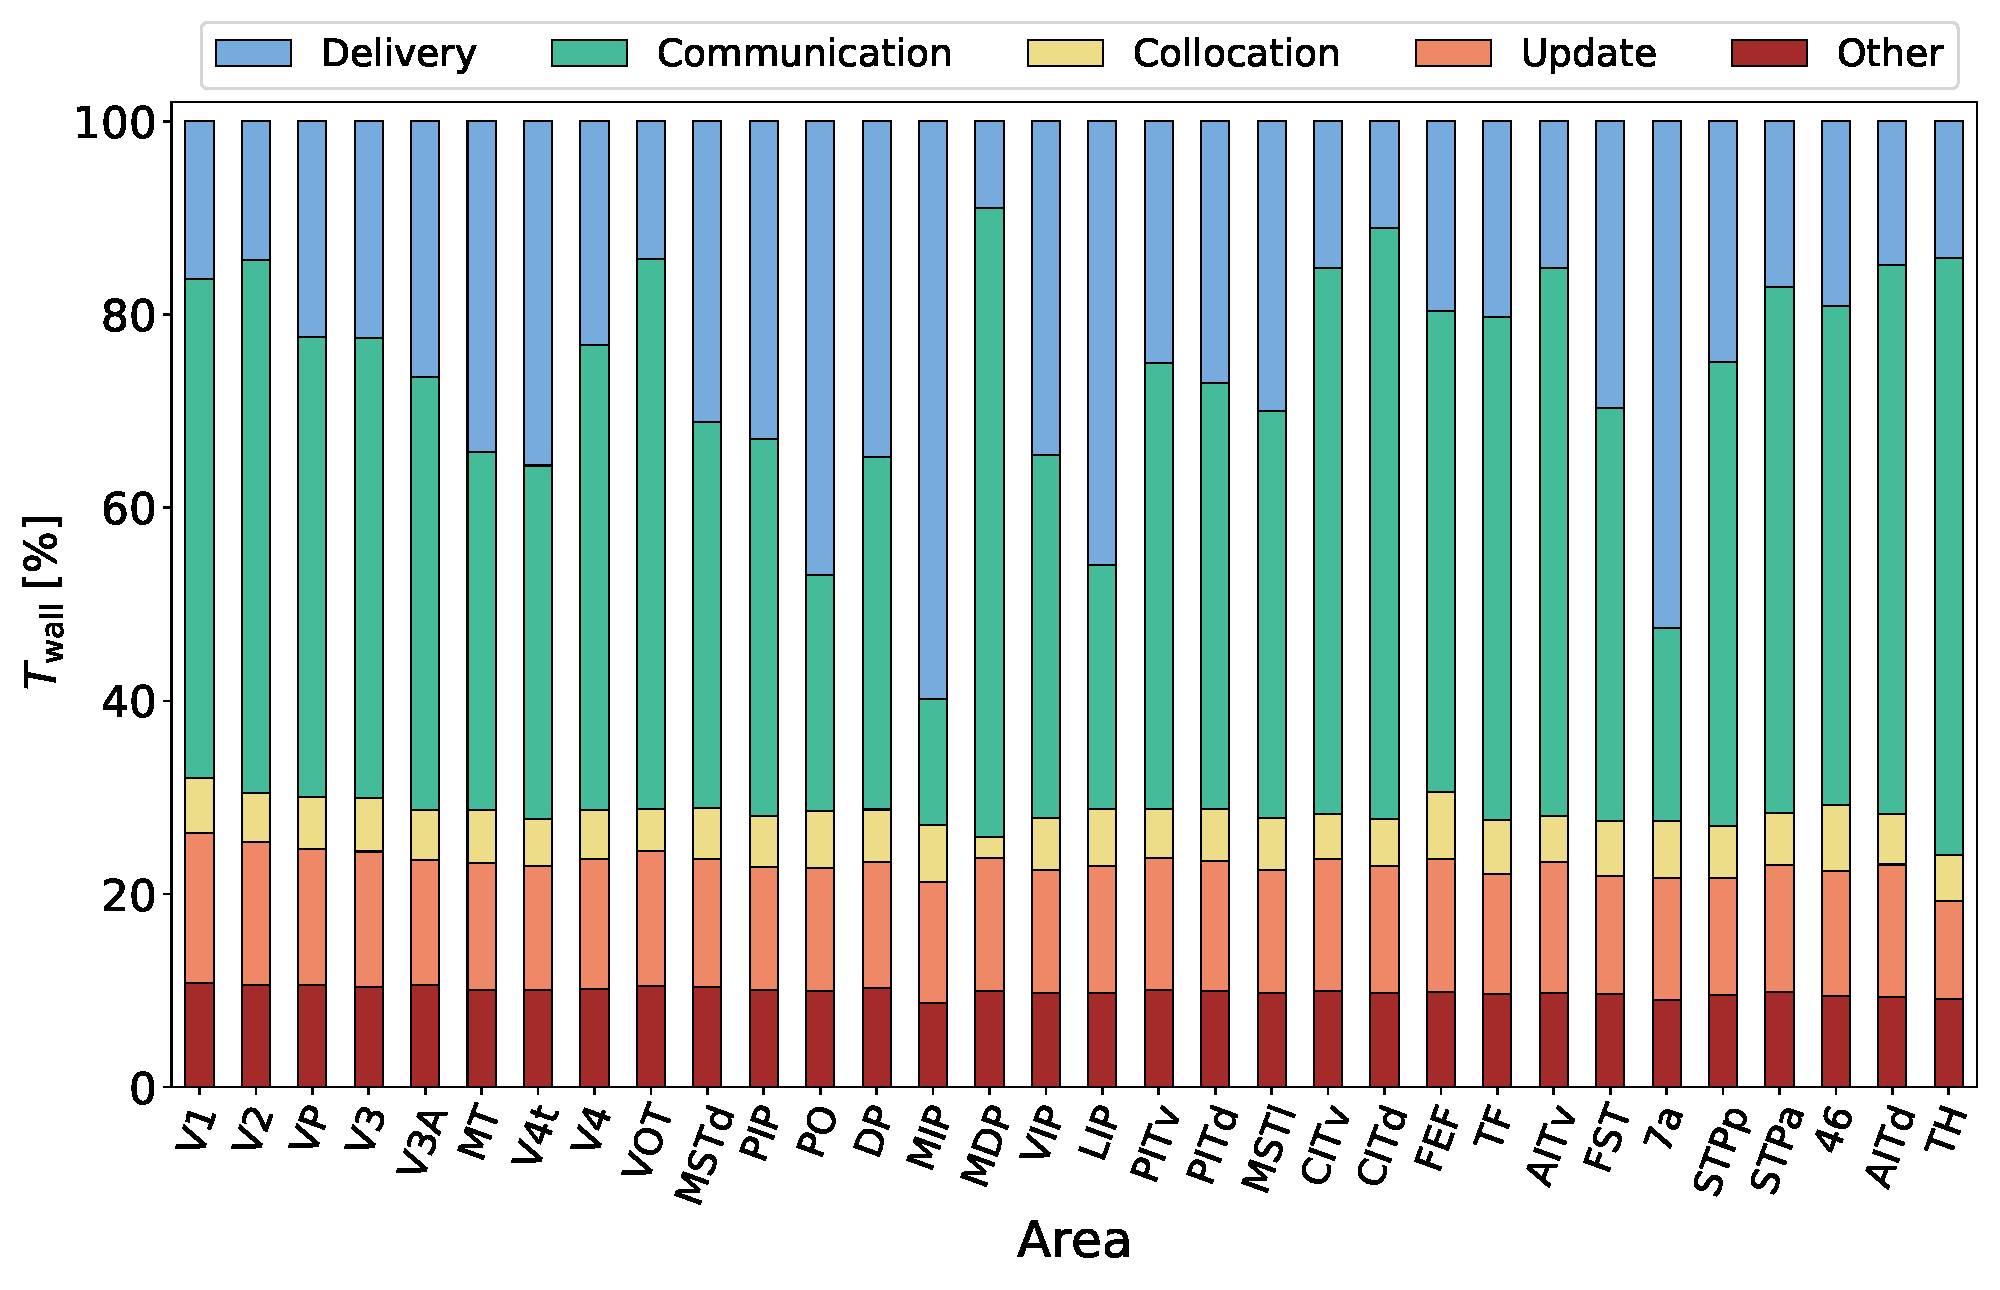
\includegraphics[width=\columnwidth]{figures/mam_sim_contributions.pdf}
    \caption{Relative contributions to the simulation time of the multi-area model in the metastable state for every area (i.e. for every MPI process) in a NEST GPU simulation.}
    \label{fig:mam_relative_contrib_sim_time}
\end{figure}

We measured that, within a simulation, the contribution of the spike communication between the 32 MPI processes (i.e. the 32 areas of the model) can vary up to 25\% with respect to its average shown in Figure \ref{fig:mam_benchmark} and the contribution of the local spike delivery subtask shows comparable variations. The rest of the subtasks (i.e. Collocation, Update and Other) do not change significantly across the MPI processes, as shown in Figure \ref{fig:mam_relative_contrib_sim_time}.
Moreover, we also evaluate the amount of spikes that have to be delivered through MPI by the multi-area model, as a fraction of the total number of spikes delivered during a simulation.\\
Figure \ref{fig:spikes_delivered} shows that the vast majority of the spikes emitted in a second of biological time are delivered within the same area, and only a small fraction of the spikes is delivered to different areas because the inter-area connections represent only a minority of the total connectivity of the model \cite{Schmidt2018}. Therefore, the NEST GPU neuron distribution, which exploits spatial locality, strongly reduce the amount of spikes that have to be carried out by communication between MPI processes and thus contribute to the
overall simulation time reduction.

\begin{figure}[h]
\centering
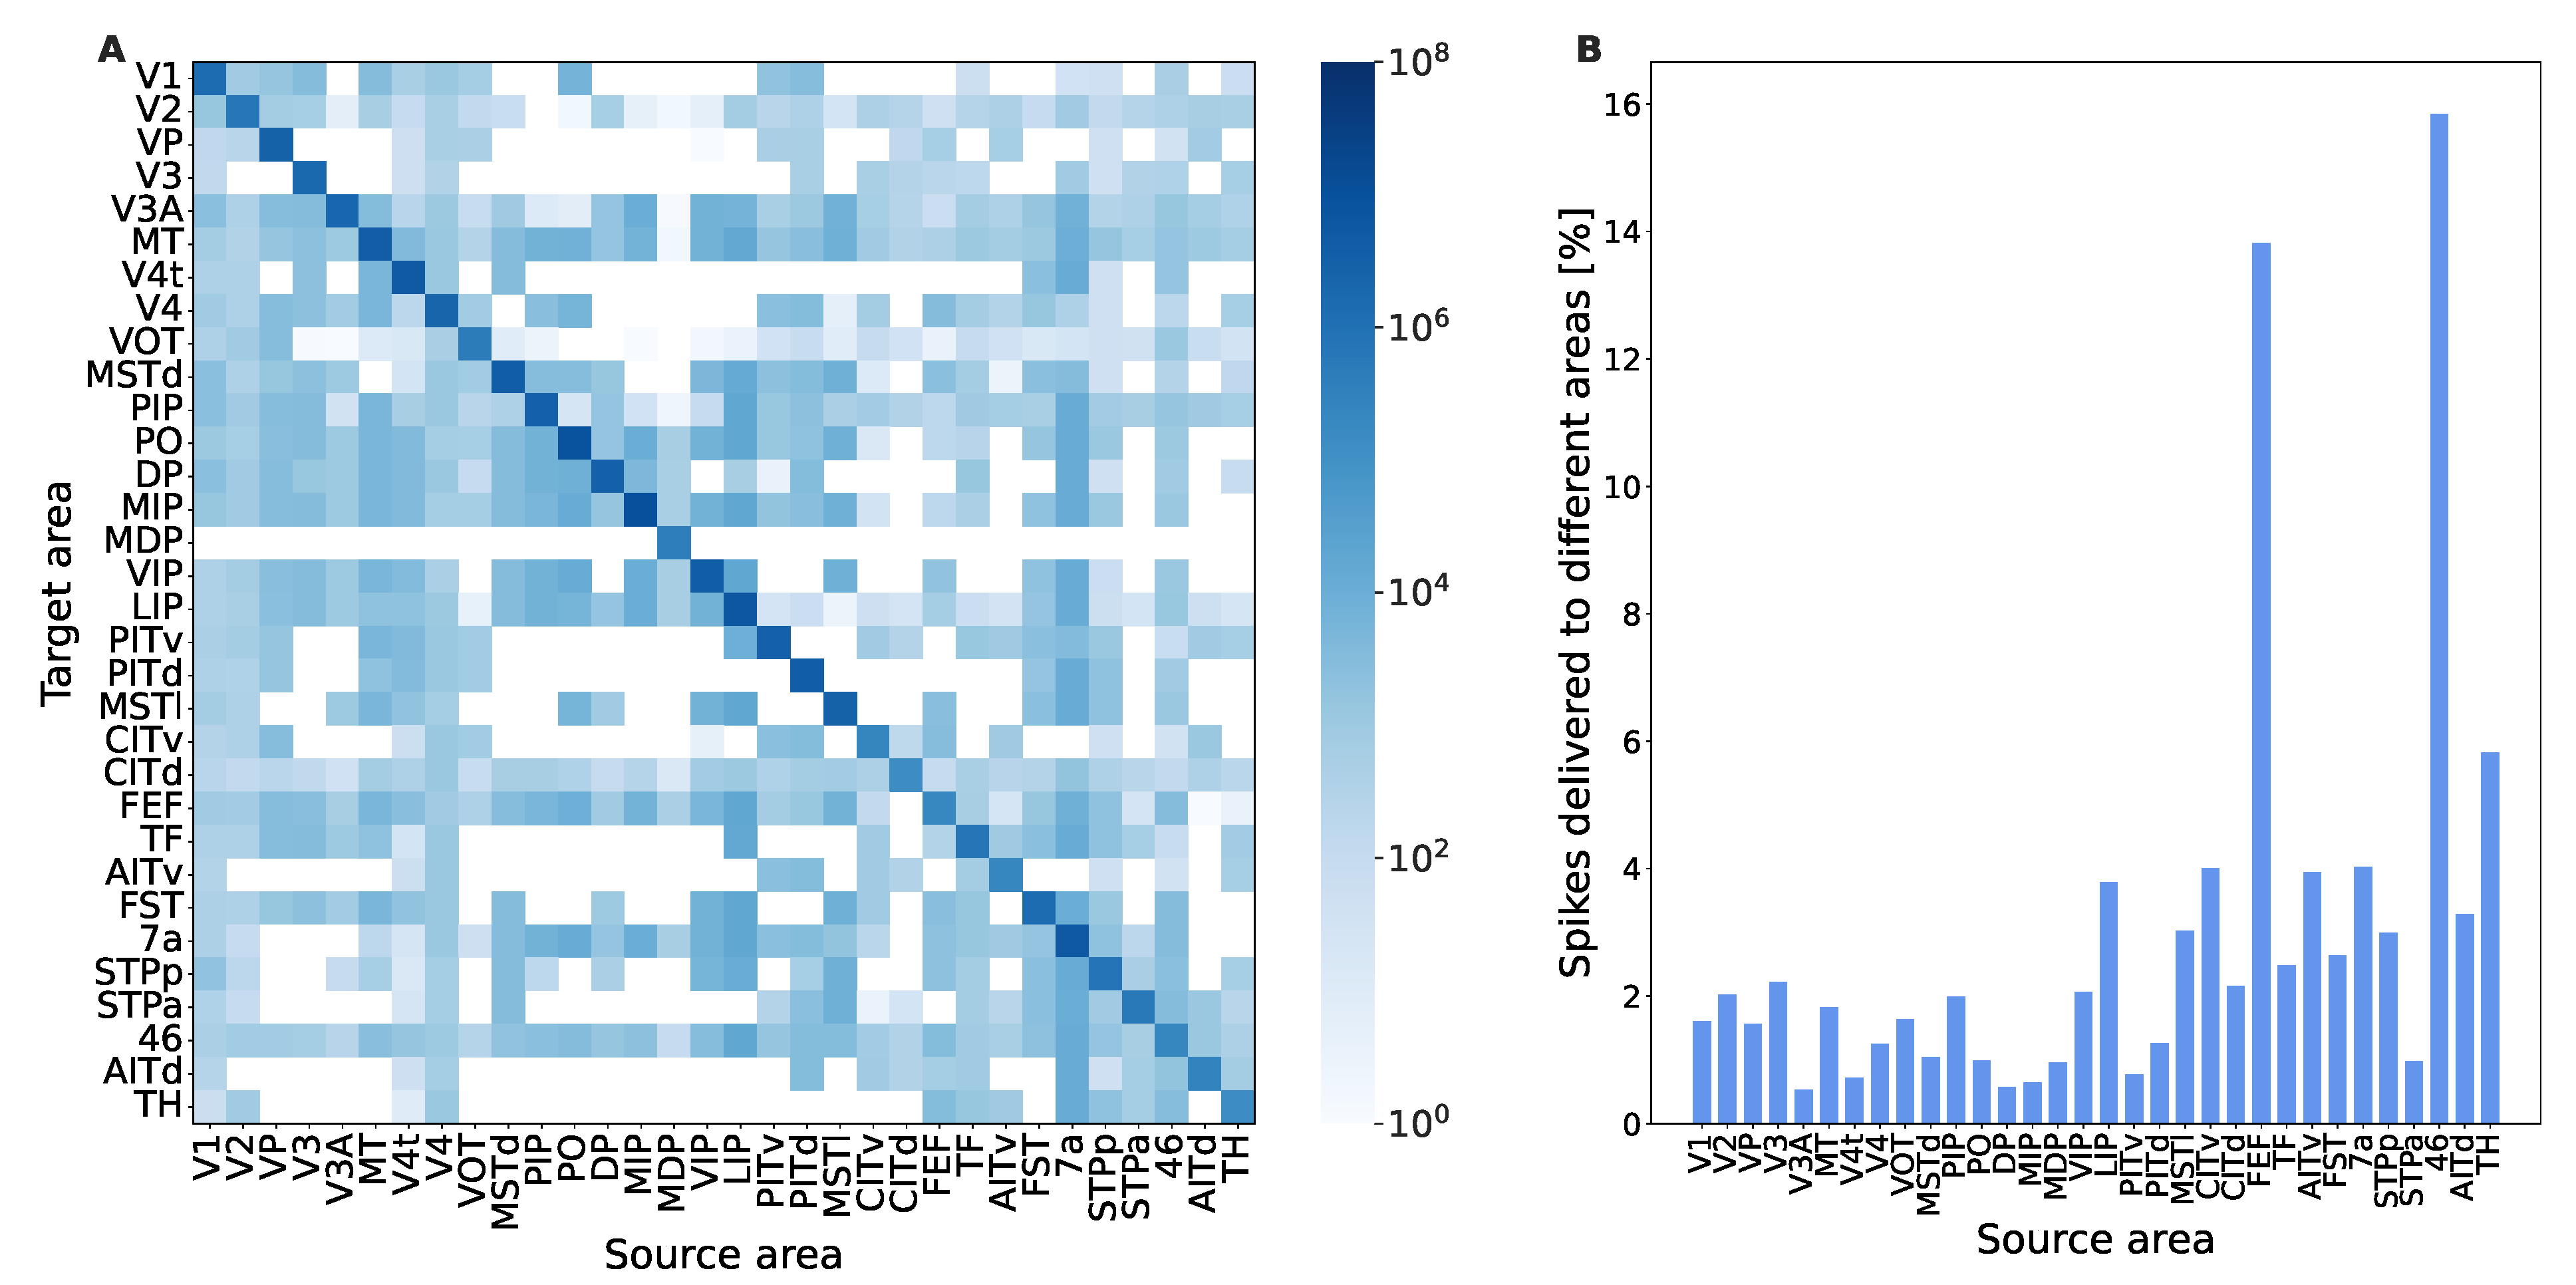
\includegraphics[width=\columnwidth]{figures/spikes_delivered.eps}
\caption{Spikes delivered in a simulation of the full-scale multi-area model in the metastable state. \textbf{(A)} Heatmap of the number of spikes delivered from each area of the model for a second of biological time. The diagonal elements show the total number of spikes fired by the neurons within the model area, whereas the off-diagonal elements show the number of spikes delivered to different areas of the model. \textbf{(B)} Fraction of spikes delivered to different areas of the model (i.e. to different MPI processes), obtained with the ratio between the number of spikes sent by a source area to every other area of the model and the total number of spikes emitted by the source area neurons. Figure from \cite{Tiddia2022}.}
\label{fig:spikes_delivered}
\end{figure}

In case of enabled spike recording using NEST GPU the simulation time increases up to 5\% when recording from all neurons. In these simulations, packing of recorded spikes and transfer to the CPU memory is performed every 2000 simulation time steps (i.e. every $200$\,ms of biological time). This overhead is strongly dependent on the model simulated and the amount of GPU memory available. Indeed, a larger GPU memory would support larger buffers of recorded spikes, diminishing the frequency of copy operations from GPU memory to CPU memory. Furthermore, the overhead can be reduced by recording spikes from only a fraction of the neurons.\\
Regarding network construction phase, the algorithm employed by NEST GPU is the one adopted by NeuronGPU. Indeed, simulations of this model reveal the limits of the previous approach: the network, both in the ground and in the metastable state, was constructed in around $955$\,s on NEST GPU (more precisely, $951\pm 29$\,s for the ground state and $957\pm 41$\,s for the metastable state), whereas the same network was constructed by NEST in around $75$\,s ($80\pm 7$\,s for the ground state and $69.5\pm 0.4$\,s for the metastable state). These results suggest that an extension of the network construction algorithm proposed in \cite{Golosio2023} for multi-GPU simulation can significantly reduce the time-to-solution when simulating large-scale model requiring an MPI-GPU cluster to be simulated. Indeed, preliminary tests suggest that an MPI implementation of this algorithm can reduce the network construction time to less than $5$\,s, but additional work is required to validate this new implementation.


\section{Simulations of the balanced network model: NEST GPU scaling performance}
In order to evaluate the scaling performance of NEST GPU, we used the balanced network model described in Section \ref{sec:balanced_network}. Indeed, the neurons or the connections per neuron simulated can differ, with a scaling that preserve the average spiking activity of the network. This way, we are able to have an idea about the times taken by the simulator to perform simulations of networks with a certain number of neurons and connections per neuron on a single GPU\footnote{Having a similar evaluation for multi-GPU simulations is an object of current work; indeed, we are currently implementing of the so-called \textit{HPC benchmark} introduced in \cite{Morrison2007}. However, this object will not be discussed in this thesis.}.\\
In particular, here we evaluate the NEST GPU scaling on the simulation of the balanced network model using the Workstation 1 described in Table \ref{tab:workstations} (i.e., the one with the NVIDIA RTX 2080 GPU). Among the compute system used, this is the most affordable one, and using a consumer-grade GPU which is not necessarily the most performing device in the market can be of broader interest for users that want to use this library on local systems.\\
The balanced network model is composed of AdEx neurons, which are integrated using the fifth-order Runge-Kutta ($5$th-RK) method with adaptive step size. Usually, the adaptive step size for GPU simulators is not used, since GPU simulations would largely benefit from fixed step size because of the SIMD parallelism. Indeed, it is not obvious a priori that a GPU simulator would be faster than a CPU-based code using this kind of integration method. Indeed, one of the next steps for the simulation of AdEx models in NEST GPU would include the possibility of using the $5$th-RK method without the adaptive step size in order to speed-up simulations with these neuron models.\\
To perform the scaling, we chose to simulate a network with $5000$ ($4000$ excitatory and $1000$ inhibitory) connections per neuron. This is a reasonable number of connections for a natural density network, which can span from few thousands to $10000$ connections per neuron. The cortical microcircuit model of \cite{Potjans2012}, for example, has on average $4000$ connections per neuron and the multi-area model of \cite{Schmidt2018} has $6000$ connections per neuron on average\footnote{These are just rough estimations; indeed, each layer or model area has a different indegree.}. The total number of neurons spans from $10000$ to $130000$. A greater amount of neurons can not be simulated for GPU memory limits, which depends on the GPU device used for simulation (here, $11$ GB). Next figure shows the weak scaling performance for the simulation of $1$\,s of biological activity of the balanced network, which shows an average firing rate of around $25$\,Hz. The results are averaged over 10 simulations using different seeds for random number generation.

\begin{figure}[H]
    \centering
    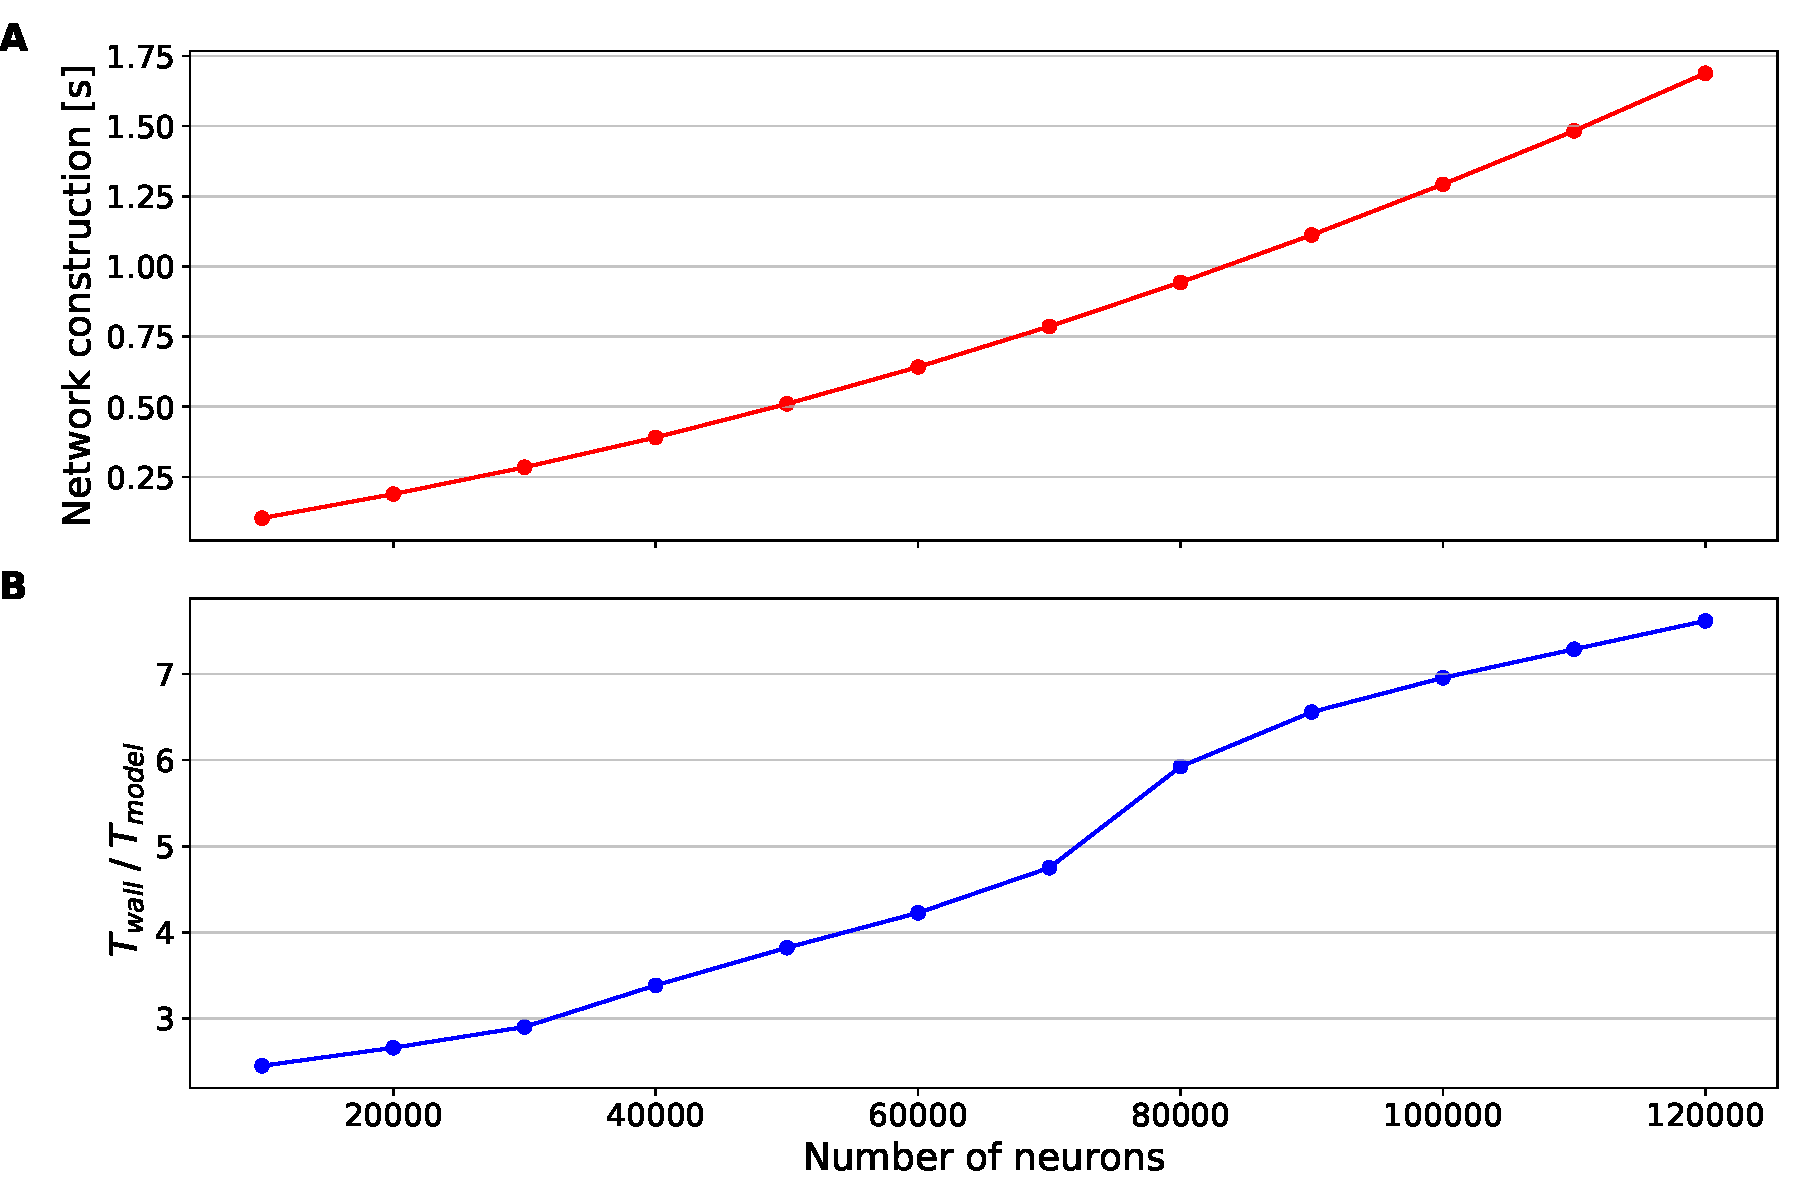
\includegraphics[width=0.9\columnwidth]{figures/weak_scaling.pdf}
    \caption{Scaling of the balanced network model for NEST GPU using a RTX 2080Ti GPU card. The network is simulated using a variable number of neurons and $5000$ connections per neuron. \textbf{(A)} Network construction time as a function of the number of neurons simulated. \textbf{(B)} Real-time factor as a function of the number of neurons. All the values are averaged over 10 simulations using different seeds.}
    \label{fig:weak_scaling}
\end{figure}

As can be seen in Figure \ref{fig:weak_scaling}, the behavior of network construction and real-time factor is approximately linear as a function of the number of neurons simulated. Moreover, when comparing these results to the one obtained in the simulation of the cortical microcircuit model (with around $80000$ neurons), we notice that the network construction is compatible with the data shown in Figure \ref{fig:cm_network_construction_ngpu}, whereas the results of the real-time factor are different from the shown in Figure \ref{fig:cm_overall_RTF}. Indeed, this is due to a different firing rate of the neurons of the simulations and also to the fact that the neuron models are different and, most importantly, integrated using different techniques. However, in this regard it is interesting to provide the performance on a type of neuron models that are integrate differently that were not used before in the simulations of the large-scale models treated here in this thesis.








%%%%%%%%%%%%%%%%%%%%%%%%%%%%%%%%%%%%%%%%%%%%%%%%%%%%%

\part{Synaptic mechanisms and cognitive processes: from the synaptic theory of Working Memory to a framework for learning through Structural Plasticity}
\label{part:II}


\chapter{\textbf{How to model Working Memory: an STP-driven spiking model}}
\label{chapter:STP_WM_model}

\begin{tcolorbox}[colback=white,colframe=DarkRed,title=\textbf{Summary}]
This chapter firstly introduces the synaptic theory of Working Memory. Then, we present and describe the reproduction of the working memory spiking network model with STP introduced in \cite{Mongillo2008}. The model has been implemented using the Python interface of the NEST simulator with the aim of paving the way for further research oriented towards the study of the relation of working memory and synaptic mechanisms.
\end{tcolorbox}


\section{Synaptic theory of Working Memory}
As discussed in Section \ref{sec:stp_wm}, Working Memory is a cognitive process which handles information manipulation and storage for a short time. Indeed, this cognitive process has a limited capacity, i.e., there is a limit on the number of items that can be kept in memory in order to manipulate them, and this number vary depending on the task that has to be performed \cite{Miller1956, cowan_2001, Cowan2010}.
The first computational models rely on attractor network dynamics to explain how neural circuits are able to encode pieces of information for a short amount of time \cite{hebb-organization-of-behavior-1949, Hopfield1982, Brunel2000}, and thus these studies were all based on the fact that these items (or \textit{chunks}) were only stored in the spiking activity of a neuron population. This fact was also grounded by experimental results on delayed-response tasks \cite{Funahashi1989, GoldmanRakic1995}, according to which the neural activity is enhanced during the delay. However, a mechanism based only on spiking activity can be biologically expensive, and experimental observations suggested also that the item can be kept in memory even after a brief interruption of the enhanced neural activity during the delay \cite{Stokes2015}. Moreover, it was observed that the higher activity during the delay takes place in the prefrontal cortex (PFC), which shows an abundance of facilitating synapses with respect to other regions of the brain \cite{Wang2006}. In 2008, the work of Mongillo et al. \cite{Mongillo2008} proposed that working memory can be sustained by a synaptic mechanism, so that an item can be stored in synaptic connections as an activity-silent event. The item can then emerge in a spiking fashion after a small stimulation \cite{Fusi2008}. The synaptic theory of working memory relies uniquely on short-term synaptic plasticity, and in particular on the mechanism of facilitating synapses, described in Section \ref{sec:STP}, related to the neurotransmitter and presynaptic calcium concentration dynamics. Facilitation leads to a short-term enhancement of synaptic efficacy in synapses that were preciously utilized (i.e. triggered by an external input) and, this way, synapses encode the item silently and retrieve it when a subsequent signal (called readout signal) is injected.


To understand the mechanism underlying the activity-silent item upkeep, let us consider a network formed by several neuron populations, each one able to encode a different item thanks to a previous learning process. When an external signal targets a neural population increasing its spiking activity, the synapses connecting neurons of the targeted population remain facilitated for a time in the order of the facilitation time constant $\tau_f$.
The connections between neurons inside the pre-stimulated population are potentiated because of prior long-term Hebbian learning, and also because of the STP modulation.
On the other hand, connections between neurons belonging to other populations are relatively weaker because they lack short-term potentiation, while the connections between neurons belonging to different selective populations are weaker because they have not been previously potentiated by long-term Hebbian learning. A similar effect could be driven by random fluctuation of neuron activity, inducing an autonomous winner-take-all (WTA) mechanism, according to which the selective excitatory population with the highest firing rate stimulates the inhibitory population eliciting a suppression of the spiking activity of the other excitatory populations \cite{Coultrip1992} due to the global inhibition. Indeed, the global inhibition is granted by the non-specific inhibitory connectivity, in agreement with experimental observations \cite{Fino2011}.
This mechanism decreases the amount of available neurotransmitter in the presynaptic terminal and increases the calcium concentration across the pre-stimulated population. Since the neurotransmitter dynamics is faster than the calcium one having synaptic facilitation, the connection strength becomes large enough to trigger again the WTA mechanism. This process can be reactivated periodically, and the period of reactivation is related to the neurotransmitter dynamics and in particular to the time constant of the synaptic depression $\tau_d$.
This oscillatory behavior can last as long as the net synaptic efficacy remains above a critical level, with a spiking outcome that strongly depends on the input provided to the network.


Indeed, such a mechanism has also a lower metabolic cost than a mechanism relying on persistent activity. As shown in \cite{Attwell2001} and \cite{Lennie2003}, only about $8\%$ of the ATP consumption for a neuron emitting at $4$\,Hz is related to the mechanism STP is inspired from, whereas spike transmission accounts for around $50\%$, meaning that activity-silent mechanisms are considerably more efficient from a energy consumption point of view. Moreover, since the items are store in a synaptic fashion, a small input is enough to retrieve the memory.


The work of Mongillo was supported by spiking network simulations of integrate-and-fire neurons. In \cite{Tiddia2022_WM} we reproduced the results shown in that work, with optimal compatibility, using the NEST simulator (version 3.1) \cite{nest3.1}. The next section describes the spiking network model in detail, showing the results of the simulations and the tests performed on the network model. More details on the compatibility of the results with experimental observations are also provided.

\section{Spiking model and reproduction of the results}

\subsection{Model description}
\label{sec:wm_model_description}
For a better understanding, here is reported the system of differential equations of STP, as described in Section \ref{sec:STP}. Being $x$ the normalized amount of available resources into the presynaptic terminal and $u$ the fraction of resources used in a spike emission, and considering a synapse connecting the presynaptic neuron $i$ and the postsynaptic neuron $j$, STP is described by 

\begin{equation}
    \begin{split}
    \dfrac{du_{i,j}}{dt} &= -\dfrac{u_{i,j} - U}{\tau_f} + U(1-u_{i,j})\sum_s\delta (t-t_s^{(i)}) \\
    \dfrac{dx_{i,j}}{dt} &= \dfrac{1-x_{i,j}}{\tau_d} - u_{i,j}x_{i,j} \sum_s\delta (t-t_s^{(i)})
    \end{split}
\end{equation}

where $\delta (\cdot)$ is the Dirac delta function and the sum is over the spike times $t_s^{(i)}$ of the presynaptic neuron $i$. The synaptic modulation takes place during the spike emission, so that
\begin{equation}
    J_{i,j}(t) = J^{\text{(abs)}}_{i,j}u_{i,j}(t-\hat{\delta}_{i,j})x_{i,j}(t-\hat{\delta}_{i,j})
\end{equation}
where $J^{\text{(abs)}}_{i,j}$ is the absolute synaptic efficacy for the synapse connecting neurons $i$ to neuron $j$ and $\hat{\delta}_{i,j}$ is the synaptic delay. The synaptic efficacy is described by the product $Jux$.


Now the network model proposed in \cite{Mongillo2008} and reproduced in \cite{Tiddia2022_WM} can be described.\\
The network is composed of $N_E$ excitatory and $N_I$ inhibitory leaky integrate-and fire (LIF) neurons with exponential postsynaptic currents. The sub-threshold dynamics of the LIF neuron model is described by the differential equation
\begin{equation}
    \tau_{\text{m}} \frac{dV_{j}}{dt}=-V_{j} + R_{\text{m}} ( I_{j}^{\text{exc}}+I_{j}^{\text{inh}} + I_{\text{ext},j})
    \label{eq:lif_wm}
\end{equation}
where $\tau_{\text{m}}$ is the membrane time constant, $V_{j}$ is the neuron's membrane potential, $R_{\text{m}}$ is the membrane resistance, $I_{j}^{\text{exc}}$ and $I_{j}^{\text{inh}}$ represent the excitatory and inhibitory synaptic current received as input from the connections within the other neurons of the network and $I_{\text{ext},j}$ represents the external input to the network. 

The network external input is modeled with Gaussian white noise currents defined by the following
\begin{equation}
    I_{\text{ext},j}(t-\hat{\delta}_{j}) = \mu_{\text{ext}}+\sigma_{\text{ext}}G_k \ \text{  for } \ k\Delta t_{\text{ng}} \leq (t-\hat{\delta}_{j}) \leq (k+1)\Delta t_{\text{ng}}
    \label{eq:gaussian_white_noise}
\end{equation}
In particular, the noise is approximated by a piecewise constant current with mean $\mu_{\text{ext}}$ and standard deviation $\sigma_{\text{ext}}$, with constant current during time intervals of length $\Delta t_{\text{ng}} = 1$\,ms. Denoting the index of the time interval with $k$, for each interval the current is given by $\mu_{\text{ext}}+\sigma_{\text{ext}}G_k$, with $G_k$ a random number extracted from a standard Gaussian distribution. The term $\hat{\delta}_{j}$ indicates the delays.

The synaptic current shown in Equation \eqref{eq:lif_wm} is the sum of the contributions given by the connections with the neurons of the network, and it is characterized by excitatory and inhibitory contributions defined as $I_{j}^{\text{exc}}(t)$ and $I_{j}^{\text{inh}}(t)$ respectively.
Thus, the synaptic input for a neuron $j$ of the network, with exponential postsynaptic currents, is given by the following equations for excitatory and inhibitory currents respectively:
\begin{equation}
\begin{split}
    \tau_{\text{exc}}\dfrac{d I_{j}^{\text{exc}}}{dt} &= - I_{j}^{\text{exc}} + \sum_i \alpha J_{i,j}(t) \sum_s \delta (t-t_s ^{(i)}-\hat{\delta}_{i,j}) \\
    \tau_{\text{inh}}\dfrac{d I_{j}^{\text{inh}}}{dt} &= - I_{j}^{\text{inh}} + \sum_i \alpha J_{i,j} \sum_s \delta (t-t_s ^{(i)}-\hat{\delta}_{i,j})
    \label{eq:input_current}
\end{split}
\end{equation}
where $i$ is the index of the presynaptic neurons targeting the neuron $j$. $\tau_{\text{exc}}$ and $\tau_{\text{inh}}$ represent the time constant of the excitatory and inhibitory synaptic currents respectively. In this model $\tau_{\text{exc}}=\tau_{\text{inh}}=2$\,ms.
$\hat{\delta}_{i,j}$ is the synaptic delay for the synapse connecting neurons $i$ and $j$. All the delays are uniformly distributed between $0.1$\,ms and $1.0$\,ms.
The time dependence of the synaptic efficacy $J_{i,j}$ is only due to short-term plasticity modulation and it is described in Equation \eqref{eq:Jupdate}, whereas synapses not modulated by the STP dynamics have fixed values of $J_{i,j}$. Since in this model only the connections between excitatory neurons employ short-term plasticity, the connections with inhibitory neurons do not show a time dependent synaptic efficacy. In addition, since the synaptic efficacies $J^{\text{(abs)}}_{i,j}$ are expressed in mV, a factor $\alpha$ is needed in order to be consistent with the units of Equation \eqref{eq:input_current}. This term derives the variation of current input needed to elicit a unit of variation of the postsynaptic potential, and has been derived in Section \ref{sec:lif_additional_eqs} (see Equation \eqref{eq:PSC_over_PSP}).


The excitatory neurons are organized in $p=5$ selective populations, each of which including a fixed fraction of neurons, and a non-selective population that includes the rest of the excitatory neurons of the network. In the base model, the selective populations of excitatory neurons have no overlap, so a neuron can not belong to different selective populations. However, in an extension of the model, it is possible to simulate it with overlapping selective populations. In such a framework, the neurons belonging to each selective population are randomly chosen from the whole excitatory population, enabling the possibility of having neurons belonging to more than one selective population.

Regarding network's connectivity, short-term plasticity is implemented in all the excitatory-to-excitatory connections using the same time constants in order to show synaptic facilitation. These connections are thus characterized by the STP variables $x$ and $u$ and a weight $J$, that represents the absolute synaptic efficacy. The weights of the connections within excitatory neurons belonging to the same selective population assume a potentiated value $J_p$, emulating the result of prior long-term Hebbian learning. On the other hand, connections between excitatory neurons belonging to different selective populations, or linking a selective population with the non-selective one, are set to a baseline value $J_b$. The rest of the excitatory-to-excitatory connections have the baseline synaptic efficacy except for the 10\% of them that show the potentiated value. This percentage is expressed in the model by a factor $\gamma$. While the excitatory-to-excitatory connections show STP dynamics, the other connections are static connections with hard-coded synaptic weights. The overall connectivity is structured so that each neuron of the network receives a fixed amount of connections from the network's populations, both excitatory and inhibitory, with a non-specific inhibitory connectivity. The possibility of having more than one synapse with the same two neurons is also enabled.
A simplified scheme of the spiking network architecture is depicted in Figure \ref{fig:network_arch}. 

\begin{figure}[h]
    \centering
    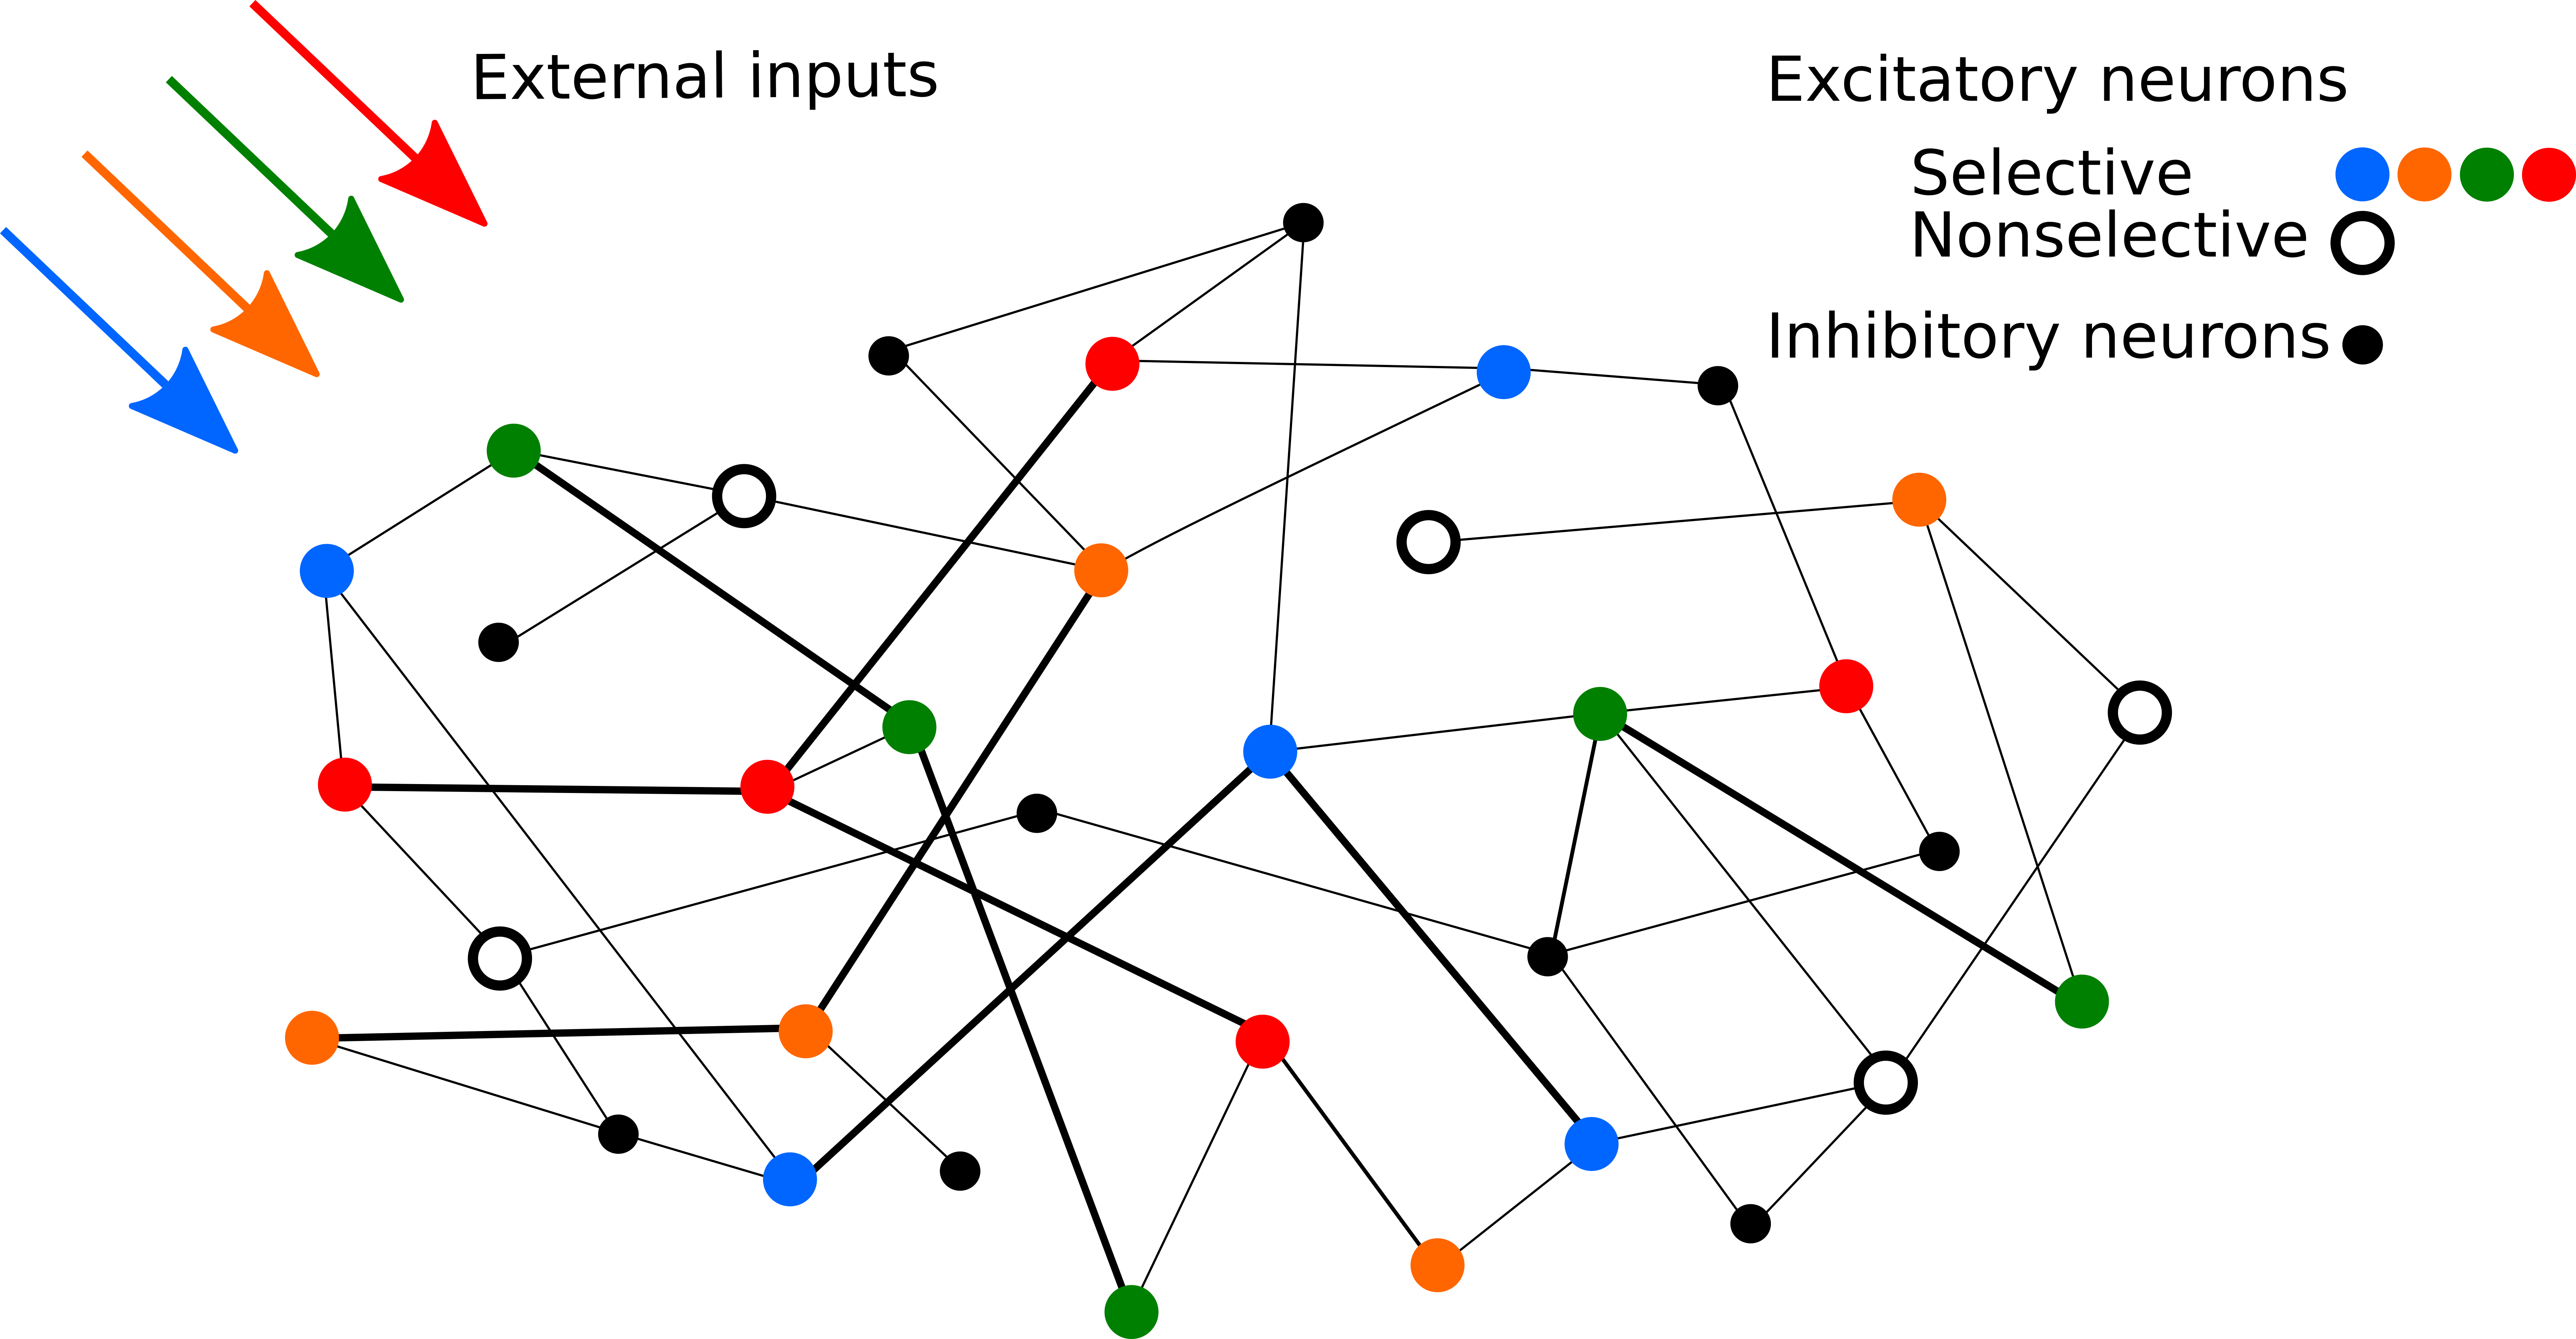
\includegraphics[width = 0.8\columnwidth]{figures/network_arch.png}
    \caption{Schematic representation of the network. Coloured circles represent excitatory neurons of different selective populations, whereas the black open circles represent excitatory neurons of the non-selective population. Black circles represent inhibitory neurons. Strengthened connections are represented by thicker black lines. Figure from \cite{Tiddia2022_WM}.}
    \label{fig:network_arch}
\end{figure}


The next tables describe, following \cite{Nordlie2009} guidelines, the network model introduced above, providing additional details on the network architecture and parameters.

\renewcommand{\arraystretch}{1.2}
%%
\begin{table}[H]
%%%%%%%%%%%%%%%%%%%
\begin{tabular}{
  |@{\hspace*{\marg}}p{0.2\textwidth}@{\hspace*{\marg}}
  |@{\hspace*{\marg}}p{0.8\textwidth}@{\hspace*{\marg}}
  |}
  \hline 
  \multicolumn{2}{|>{\color{white}\columncolor{black}}c|}{\textbf{Summary}}\\
  \hline 
  \textbf{Populations} & excitatory population $\Epop$, inhibitory population $\Ipop$\\
  \hline 
  \textbf{Connectivity} & sparse random connectivity\\
  \hline 
  \textbf{Neurons} & leaky integrate-and-fire (LIF)
  \\
  \hline 
  \textbf{Synapses} & linear input integration with exponential postsynaptic currents (PSCs),\\
  & short-term synaptic plasticity (STP) for connections between excitatory neurons\\
  \hline 
  \textbf{Input} & Gaussian white noise-like currents \\
  \hline 
\end{tabular}
\caption{Description of the network model (continues on next page).}
\label{tab:stp_wm_model}
\end{table}

\addtocounter{table}{-1}
\begin{table}[H]
%%%%%%%%%%%%%%%%%%% 
\begin{tabular}{
  |@{\hspace*{\marg}}p{0.2\textwidth}@{\hspace*{\marg}}
  |@{\hspace*{\marg}}p{0.4\textwidth}@{\hspace*{\marg}}
  |@{\hspace*{\marg}}p{0.4\textwidth}@{\hspace*{\marg}}
  |}
  \hline 
  \multicolumn{3}{|>{\color{white}\columncolor{black}}c|}{\textbf{Populations}}\\
  \hline 
  \textbf{Name} & \textbf{Elements} & \textbf{Size}\\
  \hline 
  $\Epop \equiv \Epopnonsel \cup \Epopsel \forall{}s\in \{1,\dots,p\}$  & LIF neurons & $N_\exc$\\
  \hline 
  $\Epopsel \forall{}s\in \{1,\dots,p\}$ & LIF neurons & $N_\exc\times f$\\
  \hline 
  $\Epopnonsel$ & LIF neurons & $N_\exc\times(1-fp)$\\
  \hline 
  $\Ipop$ & LIF neurons & $N_\inh$\\
  \hline 
\end{tabular}


%%%%%%%%%%%%%%%%%%%
\begin{tabular}{
  |@{\hspace*{\marg}}p{0.2\textwidth}@{\hspace*{\marg}}
  |@{\hspace*{\marg}}p{0.8\textwidth}@{\hspace*{\marg}}
  |}
  \hline 
  \multicolumn{2}{|>{\color{white}\columncolor{black}}c|}{\textbf{Neuron }}\\
  \hline 
  \textbf{Type} & leaky integrate-and-fire (LIF) dynamics\\
  \hline 
  \textbf{Description} & dynamics of membrane potential $V_{i}(t)$ and spiking activity $s_i(t)$ of neuron $i\in\left\{1,\ldots,N\right\} $:
                         \begin{itemize}
                         \item emission of $k$th ($k=1,2,\ldots$) spike of neuron $i$ at time $t_{k}^{(i)}$ if
                           \begin{equation*}
                             V_{i}\left(t_{k}^{(i)}\right)\geq\theta  
                           \end{equation*}
                           with spike threshold $\theta$;
                         \item reset and refractoriness:
                           \begin{equation*}
                             \forall{}k,\ \forall t \in \left(t_{k}^{(i)},\,t_{k}^{(i)}+\tauR\right]:\quad V_{i}(t)=V_\text{reset}  
                           \end{equation*}
                            with refractory period $\tauR$ and reset potential $V_\text{reset}$;
                         \item spike train $\displaystyle s_i(t)=\sum_k \delta(t-t_k^{(i)})$;
                         \item subthreshold dynamics of membrane potential $V_{i}(t)$:
                           \begin{equation*}
                             \begin{aligned}
                               &\forall{}k,\ \forall t \notin \left[t_{k}^{(i)},\,t_{k}^{(i)}+\tauR\right):\\
                               &\qquad\tauM\frac{\diff{}V_i(t)}{\diff{}t} =
                               \Bigl[E_\text{L}-V_i(t)\Bigr]+\RM I_i(t)
                             \end{aligned}
                           \end{equation*}
                           with membrane time constant $\tauM$, membrane resistance $\RM$, resting potential $E_\text{L}$, and total synaptic input current $I_i(t)$.
                         \end{itemize}\\
  \hline 
\end{tabular}
%%%%%%%%%%%%%%%%%%%
\caption{Description of the network model (continues on next page).}
\end{table}
%%%%%%%%%%%%%%%%%%%%%%%%%%%%%%%%%%%%%%%%%%%%%%%%%%%%%%%%%%%%%%%%%%%%%%%%%%%%%%%%%%%%
%% model description table (continues on next page)
\addtocounter{table}{-1}
\begin{table}[H]
%%%%%%%%%%%%%%%%%%% 
\begin{tabular}{
  |@{\hspace*{\marg}}p{0.15\textwidth}@{\hspace*{\marg}}
  |@{\hspace*{\marg}}p{0.15\textwidth}@{\hspace*{\marg}}
  |@{\hspace*{\marg}}p{0.7\textwidth}@{\hspace*{\marg}}
  |}
  \hline 
  \multicolumn{3}{|>{\color{white}\columncolor{black}}c|}{
  \textbf{Connectivity (part 1)}
  }\\
  \hline 
  \textbf{Source} & \textbf{Target} & \textbf{Pattern}\\
  \hline
  $\Epopsel\forall{}s\in \{1,\dots,p\}$ & $\Epopselfirst \forall{}s' \equiv s\in \{1,\dots,p\}$ & %
                      \begin{itemize}[align=left,leftmargin=*]
                      \item random, independent; homogeneous in-degree $K_{\exc,j}=fc_{\text{EEsp}}N_\exc$ ($\forall{}j\in\Epopselfirst$);
                      \item static synaptic weights $J_p$ with STP modulation ($\forall{}j\in\Epopselfirst$);
                      \item uniformly distributed spike-transmission delays $\delta_{ij} \in [0.1,1.0]$\,ms ($\forall{}i\in\Epopsel,j\in\Epopselfirst$).
                      \end{itemize}\\
  \hline
  $\Epopsel\forall{}s\in \{1,\dots,p\}$ & $\Epopselfirst \forall{}s'\neq s\in \{1,\dots,p\}$ & %
                      \begin{itemize}[align=left,leftmargin=*]
                      \item random, independent; homogeneous in-degree $K_{\exc,j}=fc_{\text{EE}}N_\exc$ ($\forall{}j\in\Epopselfirst$);
                      \item static synaptic weights $J_b$ with STP modulation ($\forall{}j\in\Epopselfirst$);
                      \item uniformly distributed spike-transmission delays $\delta_{ij} \in [0.1,1.0]$\,ms ($\forall{}i\in\Epopsel,j\in\Epopselfirst$).
                      \end{itemize}\\
  \hline
  $\Epopsel\forall{}s\in \{1,\dots,p\}$ & $\Epopnonsel$ & %
                      \begin{itemize}[align=left,leftmargin=*]
                      \item random, independent; homogeneous in-degree $K_{\exc,j}=fc_{\text{EE}}N_\exc$ ($\forall{}j\in\Epopnonsel$);
                      \item static synaptic weights $J_b$ with STP modulation ($\forall{}j\in\Epopnonsel$);
                      \item homogeneous spike-transmission delays $d_{ij}=d$ ($\forall{}i\in\Epopsel,j\in\Epopnonsel$).
                      \end{itemize}\\
  \hline
  $\Epopnonsel$ & $\Epopnonsel \lor \Epopsel\forall{}s\in \{1,\dots,p\}$ & %
                      \begin{itemize}[align=left,leftmargin=*]
                      \item random, independent; homogeneous in-degree $K_{\exc,j}=c_{\text{EE}}(1-fp)N_\exc$ ($\forall{}j\in\Epopsel$);
                      \item static synaptic weights $J_b$ with STP modulation ($\forall{}j\in\Epopsel$);
                      \item homogeneous spike-transmission delays $d_{ij}=d$ ($\forall{}i\in\Epopnonsel,j\in\Epopsel$).
                      \end{itemize}\\
  \hline 
  \end{tabular}
%%%%%%%%%%%%%%%%%%%
\caption{Description of the network model (continues on next page).}
\end{table}
%%%%%%%%%%%%%%%%%%%%%%%%%%%%%%%%%%%%%%%%%%%%%%%%%%%%%%%%%%%%%%%%%%%%%%%%%%%%%%%%%%%%
%% model description table (continues on next page)
\addtocounter{table}{-1}
\begin{table}[H]
%%%%%%%%%%%%%%%%%%% 
\begin{tabular}{
  |@{\hspace*{\marg}}p{0.15\textwidth}@{\hspace*{\marg}}
  |@{\hspace*{\marg}}p{0.15\textwidth}@{\hspace*{\marg}}
  |@{\hspace*{\marg}}p{0.7\textwidth}@{\hspace*{\marg}}
  |}
  \hline 
  \multicolumn{3}{|>{\color{white}\columncolor{black}}c|}{
  \textbf{Connectivity (part 2)}
  }\\
  \hline 
  \textbf{Source} & \textbf{Target} & \textbf{Pattern}\\
  $\Epopsel\forall{}s\in \{1,\dots,p\}$ & $\Ipop$ & %
                      \begin{itemize}[align=left,leftmargin=*]
                      \item random, independent; homogeneous in-degree $K_{\exc,j}=c_{\text{IE}}fN_\exc$ ($\forall{}j\in\Ipop$);
                      \item static synaptic weights $J_{\text{IE}}$ ($\forall{}j\in\Ipop$);
                      \item homogeneous spike-transmission delays $d_{ij}=d$ ($\forall{}i\in\Epopsel,j\in\Ipop$).
                      \end{itemize}\\
  \hline
  $\Epopnonsel$ & $\Ipop$ & %
                      \begin{itemize}[align=left,leftmargin=*]
                      \item random, independent; homogeneous in-degree $K_{\exc,j}=c_{\text{IE}}(1-fp)N_\exc$ ($\forall{}j\in\Ipop$);
                      \item static synaptic weights $J_{\text{IE}}$ ($\forall{}j\in\Ipop$);
                      \item homogeneous spike-transmission delays $d_{ij}=d$ ($\forall{}i\in\Epopsel,j\in\Ipop$).
                      \end{itemize}\\
  \hline 
  $\Ipop$ & $\Epop$ & %
                      \begin{itemize}[align=left,leftmargin=*]
                      \item random, independent; homogeneous in-degree $K_{\inh,j}=c_{\text{EI}}N_\inh$ ($\forall{}j\in\Epop$);
                      \item static synaptic weights $J_{\text{EI}}$ ($\forall{}j\in\Epop$);
                      \item homogeneous spike-transmission delays $d_{ij}=d$ ($\forall{}i\in\Ipop,j\in\Epop$).
                      \end{itemize}\\
  \hline
  $\Ipop$ & $\Ipop$ & %
                      \begin{itemize}[align=left,leftmargin=*]
                      \item random, independent; homogeneous in-degree $K_{\inh,j}=c_{\text{II}}N_\inh$ ($\forall{}j\in\Ipop$);
                      \item static synaptic weights $J_{\text{II}}$ ($\forall{}j\in\Epop$)
                      \item homogeneous spike-transmission delays $d_{ij}=d$ ($\forall{}i\in\Ipop,j\in\Ipop$).
                      \end{itemize}\\
  \hline
\multicolumn{3}{|l|}{self-connections (``autapses'') and multiple connections (``multapses'') allowed}\\
  % \hline
  % all & all & no self-connections (``autapses''), multiple connections (``multapses'') are permitted\\
  \hline
\end{tabular}
%%%%%%%%%%%%%%%%%%%
\caption{Description of the network model (continues on next page).}
\end{table}
%%%%%%%%%%%%%%%%%%%%%%%%%%%%%%%%%%%%%%%%%%%%%%%%%%%%%%%%%%%%%%%%%%%%%%%%%%%%%%%%%%%%
%% model description table (continues on next page)
\addtocounter{table}{-1}
\begin{table}[H]
%%%%%%%%%%%%%%%%%%% 
%%%%%%%%%%%%%%%%%%% 
\begin{tabular}{
  |@{\hspace*{\marg}}p{0.2\textwidth}@{\hspace*{\marg}}
  |@{\hspace*{\marg}}p{0.8\textwidth}@{\hspace*{\marg}}
  |}
  \hline 
  \multicolumn{2}{|>{\color{white}\columncolor{black}}c|}{
  \textbf{Stimulus}
  }\\
\hline 
\textbf{Type} & white noise-like Gaussian current\\
\hline 
  \textbf{Description} & External current is given by a Gaussian white noise current, with mean $\mu_{\ext}$, standard deviation $\sigma_{\ext}$ and constant current during time intervals of length $\Delta t_{\text{ng}}$. Denoting the index of the time interval with $k$, for each interval the current is given by $\mu_{\ext}+\sigma_{\ext}G_k$, with $G_k$ a random number extracted from a standard Gaussian distribution.
  \begin{equation*}
    I_{\ext,i}(t-\hat{\delta}_{i}) = \mu_{\ext}+\sigma_{\ext}G_k \text{  for } \ k\Delta t_{\text{ng}} \leq (t-\hat{\delta}_{i}) \leq (k+1)\Delta t_{\text{ng}})
  \end{equation*}
  External stimulation such as the item loading signal and the readout signal are designed in the same way and modulated using a contrast factor $\mathcal{A}$, so that the total current injected to the targeted population has mean $\mathcal{A}\mu_{\ext}$.
\end{tabular}

\begin{tabular}{
  |@{\hspace*{\marg}}p{0.2\textwidth}@{\hspace*{\marg}}
  |@{\hspace*{\marg}}p{0.8\textwidth}@{\hspace*{\marg}}
  |}
  \hline 
  \multicolumn{2}{|>{\color{white}\columncolor{black}}c|}{
  \textbf{Synapse: transmission}
  }\\
  \hline 
  \textbf{Type} & current-based synapses with exponential postsynaptic currents (PSCs)\\
  \hline 
  \textbf{Description} &
                         \begin{itemize}
                         \item total synaptic input current of neuron $i$
                         \begin{equation*}
                           I_i(t)=I_{i}^{\exc}+I_{i}^{\inh} + I_{\ext,i}
                         \end{equation*}
                       \item excitatory, inhibitory synaptic input currents
                         \begin{equation*}
                            \begin{aligned}
                              \tau_{\exc}\dfrac{d I_{i}^{\exc}}{dt} &= - I_{i}^{\exc} + \sum_i \alpha J_{i,j}(t) \sum_s \delta (t-t_s ^{(i)}-\hat{\delta}_{i,j})\\
                              \tau_{\inh}\dfrac{d I_{j}^{\inh}}{dt} &= - I_{j}^{\inh} + \sum_i \alpha J_{i,j} \sum_s \delta (t-t_s ^{(i)}-\hat{\delta}_{i,j})
                            \end{aligned}
                          \end{equation*}
                          where $\delta (t-t_s ^{(i)}-\hat{\delta}_{i,j})$ represents the spike train considering also the synaptic delay of the connections ($\hat{\delta}$). $\tau_{\exc}$ and $\tau_{\inh}$ are the excitatory and inhibitory time constants and $\alpha$ is the PSC amplitude (that gets the value of the synaptic weight in pA in order to elicit a given depolarization of the membrane potential);
                        \item PSC amplitude (synaptic weight) $\alpha$ (see Equation \eqref{eq:PSC_over_PSP}).
                         \end{itemize}                        
  \\
  \hline 
\end{tabular}
%%%%%%%%%%%%%%%%%%%
\caption{Description of the network model (continues on next page).}
\end{table}
%%%%%%%%%%%%%%%%%%%%%%%%%%%%%%%%%%%%%%%%%%%%%%%%%%%%%%%%%%%%%%%%%%%%%%%%%%%%%%%%%%%% 
%% model description table (continues on next page)
\addtocounter{table}{-1}
\begin{table}[H]
%%%%%%%%%%%%%%%%%%% 
%%%%%%%%%%%%%%%%%%% 
\begin{tabular}{
  |@{\hspace*{\marg}}p{0.2\textwidth}@{\hspace*{\marg}}
  |@{\hspace*{\marg}}p{0.8\textwidth}@{\hspace*{\marg}}
  |}
  \hline 
  \multicolumn{2}{|>{\color{white}\columncolor{black}}c|}{
  \textbf{Synapse: plasticity}
  }\\
\hline 
\textbf{Type} & short-term synaptic plasticity (STP) for connections between excitatory neurons\\
\hline 
  \textbf{Description} &
   dynamics of synaptic weights $J_{ij}(t)$ $\forall{}i\in\Epop, j\in\Epop$:
   \begin{equation*}
     \begin{aligned}
       &\forall J_{ij}\text{, given the absolute weight ($J_b$ or $J_s$ in the model,} \\ &\text{here $J^{\text{(abs)}}$ for simplicity)}: \\[1ex]
       \dfrac{du_{i,j}}{dt} &= -\dfrac{u_{i,j} - U}{\tauF} + U(1-u_{i,j})\sum_s\delta (t-t_s^{(i)}) \\
       \dfrac{dx_{i,j}}{dt} &= \dfrac{1-x_{i,j}}{\tauD} - u_{i,j}x_{i,j} \sum_s\delta (t-t_s^{(i)})\\
       J_{i,j}(t) &= J^{(abs)}_{i,j}u_{i,j}(t-\hat{\delta}_{i,j})x_{i,j}(t-\hat{\delta}_{i,j})
     \end{aligned}
   \end{equation*}
    where
    \begin{itemize}
    \item $u(t)$ and $x(t)$ are the STP variables, representing the normalized concentration of calcium ions in the presynaptic terminal and the normalized amount of neurotransmitters ready for release, respectively;
    \item $\tauD$ and $\tauF$ are the time constant for short-term depression and facilitation. In this model $\tauF\gg\tauD$;
    \item $U$ is related to the increase of calcium concentration due to the spike incoming in the presynaptic terminal;
    \item $\hat{\delta}$ is the synaptic delay.
    \end{itemize}
  \\
\hline 
\end{tabular}

\begin{tabular}{
  |@{\hspace*{\marg}}p{0.2\textwidth}@{\hspace*{\marg}}
  |@{\hspace*{\marg}}p{0.8\textwidth}@{\hspace*{\marg}}
  |}
  \hline 
  \multicolumn{2}{|>{\color{white}\columncolor{black}}c|}{
  \textbf{Initial conditions}
  }\\
\hline 
\textbf{Type} & STP parameters, membrane potential, input current\\
\hline 
  \textbf{Description} &
  \begin{itemize}
  \item STP variables: $x_{i,j}(0)=1.0$, $u_{i,j}(0)=U$;
  \item membrane potential: $V_{i}=0.0$\mV  $\quad\forall i \in \Epop, \Ipop$;
  \item input current $I_{\ext,i}=0.0$\pA $\quad\forall i \in \Epop, \Ipop$.
  \end{itemize}\\
  \hline 
\end{tabular}
%%
%%%%%%%%%%%%%%%%%%%
\caption{Description of the network model.}
\end{table}


\renewcommand{\arraystretch}{1.2}
%%
%% parameters table
\def\widthA{0.1}
\def\widthB{0.25}
\def\widthC{0.65}
\begin{table}[H]
  \begin{tabular}{
    |@{\hspace*{\marg}}p{\widthA\textwidth}@{\hspace*{\marg}}
    |@{\hspace*{\marg}}p{\widthB\textwidth}@{\hspace*{\marg}}
    |@{\hspace*{\marg}}p{\widthC\textwidth}@{\hspace*{\marg}}
    |}
    \hline 
    \multicolumn{3}{|>{\color{white}\columncolor{black}}c|}{\textbf{Network and connectivity}}\\
    \hline 
    \textbf{Name} & \textbf{Value } & \textbf{Description}\\
    \hline 
    $f$ & $0.1$ & fraction of neurons in a synaptic population\\
    \hline 
    $p$ & $5$ & number of selective populations\\
    \hline 
    $c_{\text{EEsp}}$ & $0.2$ & connectivity level for neurons belonging to the same selective population\\
    \hline 
    $c_{\text{EE}}$ & $0.2$ & connectivity level for other E$\rightarrow$E connections\\
    \hline 
    $c_{\text{IE}}$ & $0.2$ & connectivity level for E$\rightarrow$I connections\\
    \hline 
    $c_{\text{EI}}$ & $0.2$ & connectivity level for I$\rightarrow$E connections\\
    \hline 
    $c_{\text{II}}$ & $0.2$ & connectivity level for I$\rightarrow$I connections\\
    \hline
    $N_{\exc}$ & $8000$ & number of excitatory neurons\\
    \hline 
    $N_{\inh}$ & $2000$ & number of inhibitory neurons\\
    \hline 
  %%%%%%%%%%%%%%%%%%%%%%%%%%%%%%%%%%%%%%%%%%%%% 
    \multicolumn{3}{|>{\color{white}\columncolor{black}}c|}{
    \textbf{Neuron}
    }\\
    \hline 
    \textbf{Name} & \textbf{Value } & \textbf{Description}\\
    \hline 
    $V_{\text{th}}$ & $20\mV$ & spike threshold\\
    \hline 
    $E_\text{L}$ & $0\mV$ & resting potential\\
    \hline 
    $\tauM$ & $15\ms$ & membrane time constant\\
    \hline 
    $\CM$ & $250\pF$ & membrane capacitance\\
    \hline
    $V_\text{reset}$ & $0\mV$ & reset potential\\
    \hline 
    $\tauR$ & $2\ms$ & absolute refractory period\\
    \hline
  %%%%%%%%%%%%%%%%%%%%%%%%%%%%%%%%%%%%%%%%%%%%% 
    \multicolumn{3}{|>{\color{white}\columncolor{black}}c|}{
    \textbf{Synapse}
    }\\
    \hline 
    \textbf{Name} & \textbf{Value } & \textbf{Description}\\
    %%%%%%%%%%%%%%%%%%%%
    %% transmission
    \hline
    $J_{\text{b}}$ & $0.10\,\mV$ & baseline weight (PSP amplitude) for excitatory to excitatory synapses\\
    \hline
    $J_{\text{p}}$ & $0.45\,\mV$ & potentiated weight of excitatory to excitatory synapses\\
    \hline
    $J_{\text{IE}}$ & $0.135\,\mV$ & weight of excitatory to inhibitory synapses\\
    \hline
    $J_{\text{EI}}$ & $0.25\,\mV$ & weight of inhibitory to excitatory synapses\\
    \hline
    $J_{\text{II}}$ & $0.2\,\mV$ & weight  of inhibitory to inhibitory synapses\\
    \hline 
    $\gamma_0$ & $0.0$ & fraction of potentiated synapses across different excitatory sub-populations\\
    \hline
    $\hat{\delta}$ & $\mathcal{U}(0.1, 1.0) \ms$ & synaptic delays uniformly distributed\\
    \hline
    $U$ & $0.19$ & baseline STP utilization factor\\
    \hline
    $u$ & $U$ & (initial) fraction of resources released for a spike\\
    \hline
    $x$ & $1.0$ & (initial) fraction of resources ready to be released\\
    \hline
    $\tauF$ & $1500.0\ms$ & facilitation time constant\\
    \hline
    $\tauD$ & $200.0\ms$ & depression time constant\\
    \hline
    %%%%%%%%%%%%%%%%%%%%%%%%%%%%%%%%%%%%%%%%%%%%%
    \end{tabular}
%%%%%%%%%%%%%%%%%%%
\caption{Model parameters (continues on next page).}
\label{tab:stp_wm_params}
\end{table}
%%%%%%%%%%%%%%%%%%%%%%%%%%%%%%%%%%%%%%%%%%%%%%%%%%%%%%%%%%%%%%%%%%%%%%%%%%%%%%%%%%%%
%% model description table (continues on next page)
\addtocounter{table}{-1}
\begin{table}[H]
%%%%%%%%%%%%%%%%%%% 
\begin{tabular}{
    |@{\hspace*{\marg}}p{\widthA\textwidth}@{\hspace*{\marg}}
    |@{\hspace*{\marg}}p{\widthB\textwidth}@{\hspace*{\marg}}
    |@{\hspace*{\marg}}p{\widthC\textwidth}@{\hspace*{\marg}}
    |}
  \hline 
    \multicolumn{3}{|>{\color{white}\columncolor{black}}c|}{
    \textbf{Stimulus}
    }\\
    \hline 
    \textbf{Name} & \textbf{Value } & \textbf{Description}\\
    \hline
    $\eta_{\ext}^{\exc}$ & variable  & mean external current for excitatory neurons\\
    \hline
    $\eta_{\ext}^{\inh}$ & $20.5$\mV  & mean external current for inhibitory neurons\\
    \hline
    $\Sigma_{\ext}^{\exc}$ & $1.0$\mV  & standard deviation of external current for excitatory neurons\\
    \hline
    $\Sigma_{\ext}^{\inh}$ & $1.0$\mV  & standard deviation of external current for inhibitory neurons\\
    \hline
    $\mathcal{T}_{\text{cue}}$ & $350.0$\ms  & item loading signal duration\\
    \hline
    $\mathcal{A}_{\text{cue}}$ & $1.15$  & item loading signal contrast factor\\
    \hline
    $\mathcal{T}_{\text{reac}}$ & $250.0$\ms  & readout signal duration\\
    \hline
    $\mathcal{A}_{\text{reac}}$ & $1.05$  & readout signal contrast factor\\
    \hline
    $\mathcal{T}_{\text{reac}}^{\text{period}}$ & $100.0$\ms  & periodic readout signal duration\\
    \hline
    $\mathcal{A}_{\text{reac}}^{\text{period}}$ & $1.075$  & periodic readout signal contrast factor\\
    \hline
  %%%%%%%%%%%%%%%%%%%%%%%%%%%%%%%%%%%%%%%%%%%%%
  \end{tabular}
  \caption{Model parameters.}
\end{table}

In the previous Table are illustrated the synaptic parameters used in this spiking network model to build the external stimuli. It should be noted that the external stimulus, modeled as a Gaussian white noise current, shows mean $\eta_{ext}$ and standard deviation $\Sigma_{ext}$ expressed in mV and not in pA. In \cite{Tiddia2022_WM} we derived\footnote{We followed the derivation of the NEST Documentation, please see \url{https://nest-simulator.readthedocs.io/en/v3.1/model_details/noise_generator.html?highlight=noise_generator##Hans-Ekkehard-Plesser,-2015-06-25}} that, given the mean $\mu$ and standard deviation $\sigma$ of a piecewise constant current injected to a neuron, with standard deviation changing at fixed intervals of length $\Delta t_{\text{ng}}$, the membrane potential will show a mean $\eta$ and the standard deviation $\Sigma$ described as follows:

\begin{equation}
    \begin{split}
        \eta &= \mu \dfrac{C_m}{\tau_m} \\
        \Sigma &= \sqrt{\dfrac{2}{\tau_{\text{m}} \Delta t_{\text{ng}}}} C_{\text{m}} \sigma
    \end{split}
    \label{eq:noise_generator}
\end{equation}

\subsection{Results of the simulation}
In this section we present the results of the spiking network simulations performed using the  NEST simulator \cite{nest3.1}.

The network is composed of 8000 excitatory and 2000 inhibitory LIF neurons with exponential postsynaptic currents, whose dynamics is described by Equations \eqref{eq:lif_wm}, \eqref{eq:gaussian_white_noise} and \eqref{eq:input_current} (see also Equations 1, 2, 4 and 5 in \cite{Burkitt2006} and Equation 3 in \cite{Hanuschkin2010}). The neuron model differs from the one employed in the original work, as in \cite{Mongillo2008} is employed a LIF neuron model with instantaneous rise and decay times for postsynaptic currents. As shown in Tables \ref{tab:stp_wm_model} and \ref{tab:stp_wm_params}, the excitatory population is further divided into $p=5$ selective populations of 800 neurons each and a non-selective population that includes the rest of the excitatory neurons. All excitatory-to-excitatory connections follow a STP dynamics whereas the rest of the connections have fixed synaptic efficacies.

The simulations are performed using a time step of $0.05$\,ms, with the system of Equation \eqref{eq:lif_wm} and Equation \eqref{eq:input_current} integrated following the exact integration scheme of \cite{Rotter1999} and assuming that the external current $I_{\text{ext},j}$ is piecewise constant over time intervals of width $\Delta t_{\text{ng}}$. This is an additional difference with respect to \cite{Mongillo2008}, in which both Equation \eqref{eq:lif_wm} describing the neuron sub-threshold dynamics and Equation \eqref{eq:STP} describing the STP mechanism are integrated using the Euler scheme. Indeed, the implementation here adopted is also different from the NEST default implementation\footnote{The NEST version provided with the synapse model used here can be found at \url{https://github.com/gmtiddia/nest-simulator-3.1}.}. Further details on these differencies are described in Appendix \ref{app:STP_implementation}.
In this model the STP timescales are set so that the network shows synaptic facilitation, in fact $\tau_d = 200$\,ms and $\tau_f = 1500$\,ms in agreement with the parameters chosen in \cite{Mongillo2008}. 


All the simulations begin with a time period of $3000$\,ms in which only the background input is injected into the whole network in order to allow the network to enter its baseline state illustrating spontaneous activity. This stimulation, as well as all the other external signals, is created using the NEST \texttt{noise\_generator}, which injects a Gaussian white noise current as described in Equation \eqref{eq:gaussian_white_noise}. The background input targets both excitatory and inhibitory neurons with different mean current values. Later in this section it will be shown how network behavior can be modulated by changing excitatory background activity.


After the network reaches its spontaneous activity, an additional current, designed as a Gaussian white noise current which sums up to the background input, is injected only into a selective population for a time $\mathcal{T}_{\text{cue}}=350$\,ms. As a result, an item is re-loaded into the model. This signal, called item loading, increases the synaptic activity of the target population and thus permits a temporary strengthening of synaptic efficacies by changing the STP variables $u$ and $x$ across the connections of neurons belonging to the target population. Thus, even after the end of the item loading signal, the reloaded memory can be synaptically facilitated especially because of the slow decaying dynamics of the variable $u$. The next figure shows the raster plot for two selective populations when an item is loaded in one of them, having different values of background input.

As can be seen in Figure \ref{fig:figure2}, the memory-specific response of the network depends on the background activity level of the excitatory neurons. This figure shows the raster plot of two selective populations, one targeted by the additional current which re-loads the item and a non-targeted one, together with the STP variables $x$ and $u$ averaged over the connections outbound from the neurons of the targeted selective population. In Figure \ref{fig:figure2}A, to reactivate a memory, a supplemental external signal targeting the entire excitatory population is given. Although this external signal is nonspecific, only the population in which the memory was previously restored responds with the emission of a single synchronized activity, called \textit{population spike}. The network can also autonomously exhibit a memory-specific spiking activity when a higher excitatory background current is injected (see Figure \ref{fig:figure2}B and \ref{fig:figure2}C). 

\begin{figure}[H]
    \centering
    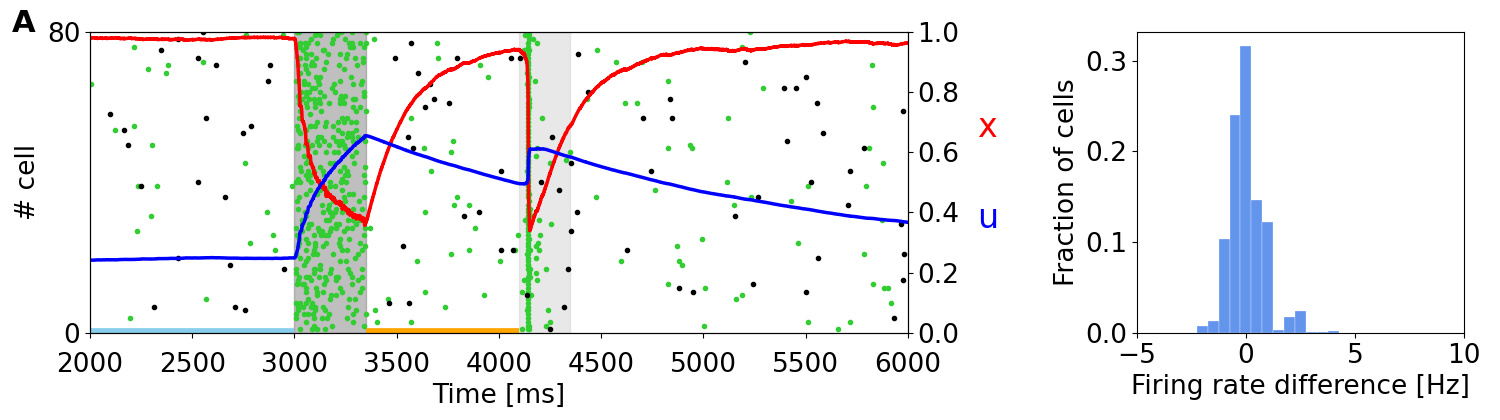
\includegraphics[width=0.9\columnwidth]{figures/fig2A.png}
    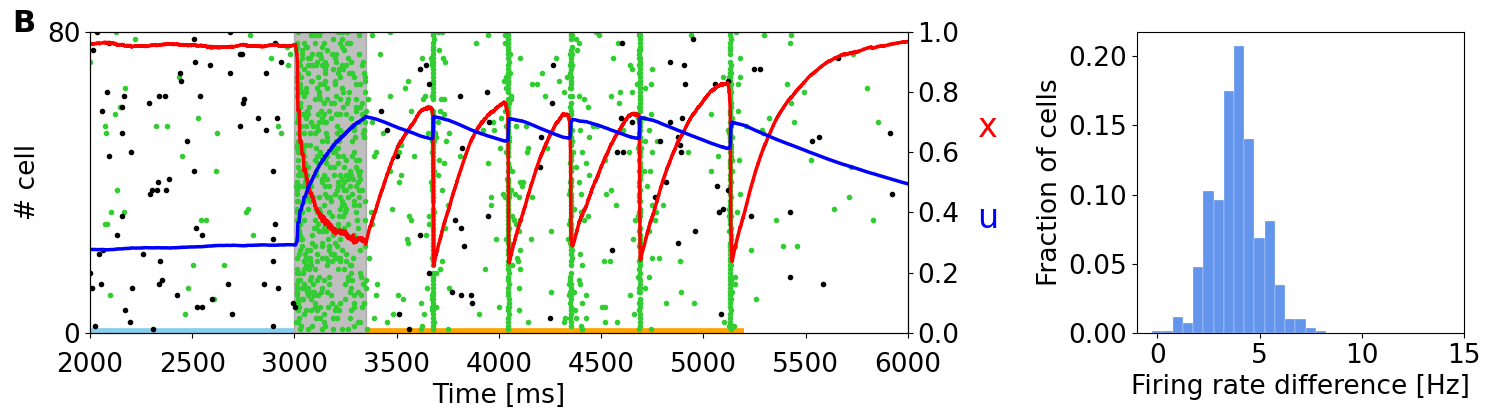
\includegraphics[width=0.9\columnwidth]{figures/fig2B.png}
    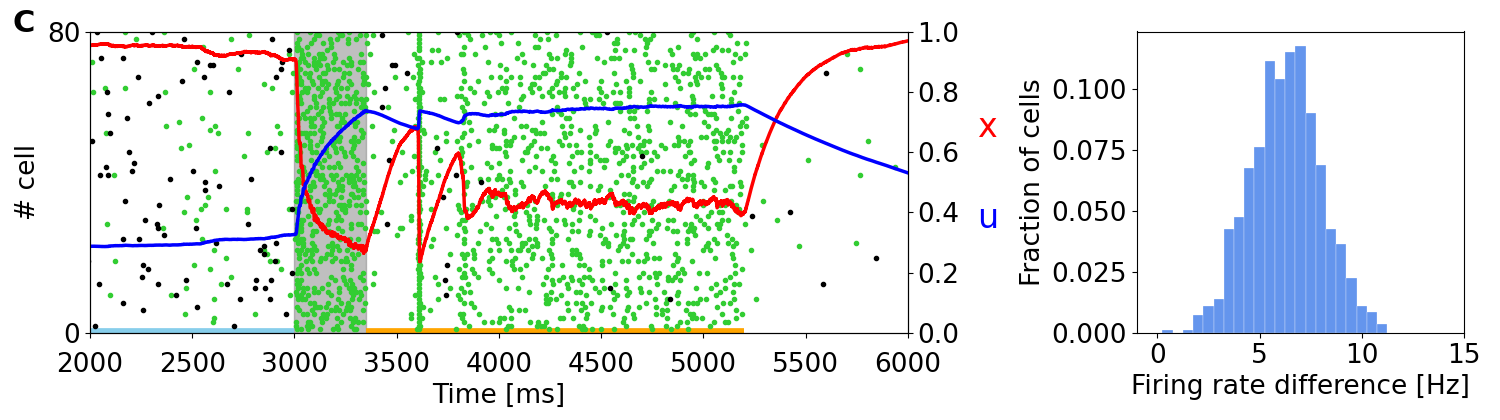
\includegraphics[width=0.9\columnwidth]{figures/fig2C.png}
    \caption{Raster plots of a subset of neurons of a targeted (green) and non-targeted (black) selective population for different values of excitatory background input. Averaged STP variables ($x$ in red and $u$ in blue) of the synaptic connections belonging to the target population are also shown. \textbf{(Left)} \textbf{(A)} The network needs the injection of a nonspecific input (lighter gray shading) to show a memory-specific response. \textbf{(B)} Increasing the background input, the network autonomously reactivates the memory by showing periodic synchronized events. \textbf{(C)} With a further increase in the background stimulus, the network shows an asynchronous enhanced spiking activity of the re-loaded memory. In (B) and (C), the network returns to its spontaneous state when background input diminishes. \textbf{(Right)} Histograms representing the difference in firing rate between the delay period (orange line at the bottom of the left panels) and the spontaneous state for the selective population targeted by the item loading signal (sky blue line at the bottom of the panels). In (A) the delay period is defined as the time between the end of item loading stimulus and the beginning of the nonspecific external input, whereas in (B) and (C) is the time between the end of item loading and the decreasing of the external background input (here at $5.2$\,s). Figure from \cite{Tiddia2022_WM}.}
    \label{fig:figure2}
\end{figure}

In Figure \ref{fig:figure2}B the targeted selective population shows an autonomous and synchronous emission of population spikes. It should be noted that after each population spike the STP variable $u$ increases and returns to similar values reached at the end of the item loading signal injection, interrupting the exponential decrease due to calcium removal mechanism and thus enabling a new population spike to emerge. This behavior, together with the fast exponential growth of available resources described by the variable $x$, lead to a new stable state for the network together with the one representing spontaneous activity. To interrupt the network persistent activity we set the excitatory background current to the value of Figure \ref{fig:figure2}A. In Figure \ref{fig:figure2}C the background input is further increased, and the network spontaneously shows an asynchronous higher rate activity. In this state the memory is maintained in a both spiking and synaptic form since the STP parameters reach stable values during the high activity state followed by a population spike. 
As in the previously described state, the network could pass from the memory specific activity state to the spontaneous state by diminishing the background input. Indeed, without the diminishing of the background input, the network would continue to behave showing the asynchronous higher rate activity or the synchronous emission of population spikes. The values of the mean excitatory background current (i.e., $\eta_{\text{X}^{\text{E}}}$) used in Figure \ref{fig:figure2} are $22.7$\,mV, $23.7$\,mV and $24.1$\,mV  respectively for the panels A, B and C.


Moreover, we quantitatively estimate the difference of firing rate for the targeted selective population between the delay period and the spontaneous activity state. The difference of firing rate for a neuron population is obtained by measuring the spike-count rate for each neuron of the population in two time intervals. Naming $r_s$ the firing rate measured during the spontaneous activity state and $r_d$ the firing rate measured during the delay period, the firing rate difference for a neuron $i$ of the population is 
\begin{equation}
    \Delta r^{(i)} = r^{(i)}_d - r^{(i)}_s = \frac{N^{(i)}_d}{\Delta t_d} - \frac{N^{(i)}_s}{\Delta t_s}
\end{equation}
where $N^{(i)}$ is the number of spikes emitted by the neuron $i$ in a certain time interval $\Delta t$. Those values are obtained for each neuron of the targeted selective population and are collected in the histograms on the right side of Figure \ref{fig:figure2}. In panel \ref{fig:figure2}A the delay period is defined as the time between the end of item loading and the beginning of the nonspecific signal, whereas in the other panels is identified between the end of the item loading and the decreasing of the external input (happening at $5.2$\,s for both panels). The time intervals related to the spontaneous activity and the delay period are indicated with horizontal lines (sky blue and orange respectively) in the left panels of Figure \ref{fig:figure2}. It is possible to notice that in panel \ref{fig:figure2}A there is no significant difference in firing rate, and a relevant part of the network shows a decrease in firing rate during the delay period. In panels \ref{fig:figure2}B and \ref{fig:figure2}C is observed an increase in firing rate of about $4$\,Hz and $7$\,Hz respectively, with an average baseline firing rate of about $0.7$\,Hz. These changes in firing rate are lower with respect to the ones shown in network models relying only to persistent activity to show working memory behavior such as \cite{Brunel2000} and they are in agreement with experimental measures on single-cell activity during delay period \cite{Shafi2007}, according to which the changes in firing rate are mostly below $5$\,Hz.


In comparison with the work of \cite{Mongillo2008}, the network simulated with NEST shows qualitatively similar results, with comparable behavior when modulating the background input targeting the excitatory neurons. However, we noticed some relevant differences with respect to the original work.
For instance, on the left side of Figure \ref{fig:figure2}B, it is possible to see that the time interval between adjacent population spikes is around $300$\,ms, whereas in \cite{Mongillo2008} this value is closer to $200$\,ms, same order of $\tau_d$. Further, while the behavior of the variable $u$ is mostly comparable to the one shown in the original article, the behavior of the variable $x$ shows a considerably higher drop of the averaged variable in correspondence to a population spike. This pronounced drop in the value of $x$ is probably the reason for the difference in the time interval between two population spikes previously mentioned. 


Since one of the main features of a working memory network is the holding of multiple information, we load two items into two different selective populations at different times to analyze the behavior of the STP variables of the targeted populations and the capacity of such a network of maintaining multiple items. In Figure \ref{fig:figure3} it is shown a subset of two selective populations targeted by the item loading signal in the single stable state regime (Figure \ref{fig:figure3}A) and in the regime showing synchronous and autonomous reactivation (Figure \ref{fig:figure3}B), obtained using the same values of background input used in Figure \ref{fig:figure2}A and Figure \ref{fig:figure2}B respectively.

Moreover, both the simulations are provided with noise, injected to a fraction of all the excitatory neurons in order to check the robustness of the network state. The noise signal is designed as the item loading one, but targets the $15$\% of the excitatory neurons randomly. In Figure \ref{fig:figure3}A the reactivation of the selective populations is enabled by a periodic nonspecific input (with a period of $300$\,ms). It can be noticed that in this framework the two targeted selective populations do not emit the population spike during the same periodic readout signal, but they alternate in order to reach suitable values of STP variables to enable the emission of a population spike in the following readout signal. This peculiar behavior can be seen also when the network autonomously shows the synchronous spiking activity (Figure \ref{fig:figure3}B). In this case, similarly to Figure \ref{fig:figure3}A, the synchronous activity of the targeted selective populations is alternated, increasing the average value of $x$ for a population when the other one is emitting the population spike. However, in Figure \ref{fig:figure3}B, this mechanism is completely autonomous. In both the network states the slow dynamics of $u$ has a key role in holding the information, in particular when another selective population shows a higher spiking activity. In addition, it can be observed that the higher spiking activity of a selective population inhibits the other populations. This is due to the network’s connectivity which enables a winner-take-all mechanism, i.e. the competition between different populations through a mechanism of global inhibition, as previously described. For this reason, it is not possible to correctly load multiple items at the same time and it is not possible to have population spikes from different selective populations at the same time. As can be seen in Figure \ref{fig:figure3}A, even if the readout signal targets all the selective populations, only the targeted selective population which has the highest STP-modulated synaptic efficacy is capable of emitting a population spike, inhibiting the excitatory neurons of the competing selecting populations.

\begin{figure}[H]
    \centering
    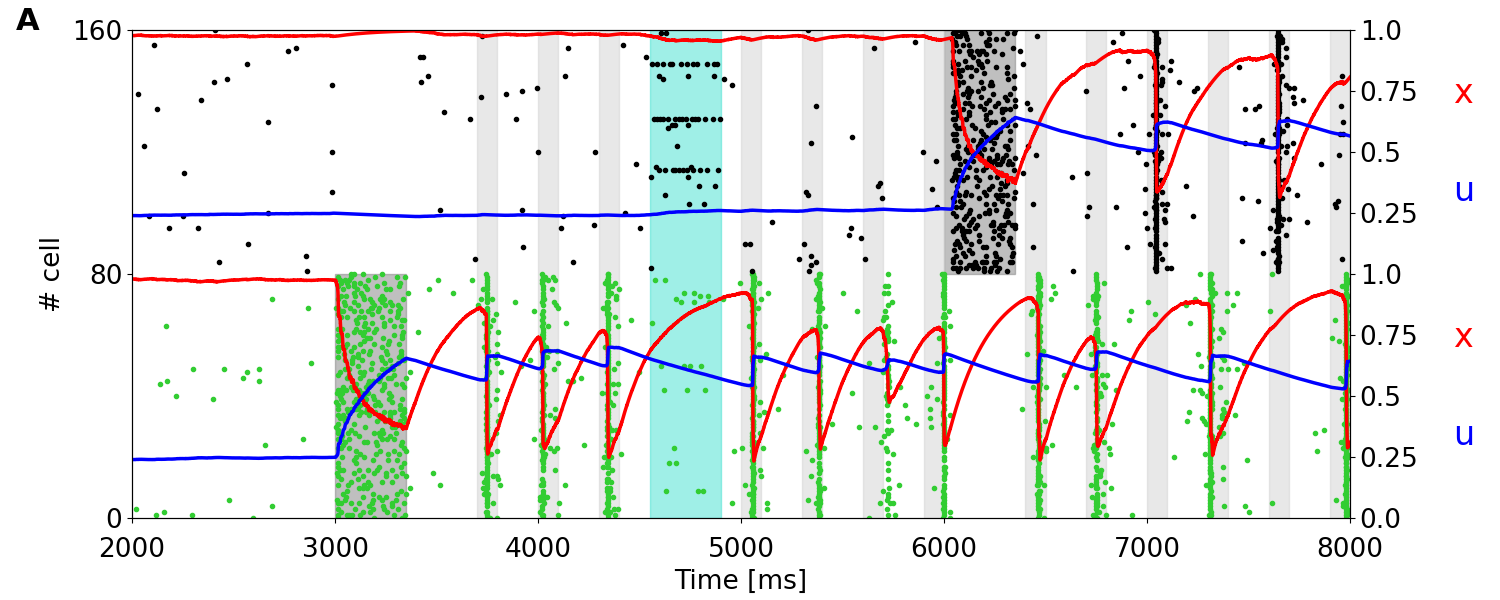
\includegraphics[width=0.9\columnwidth]{figures/fig3A.png}
    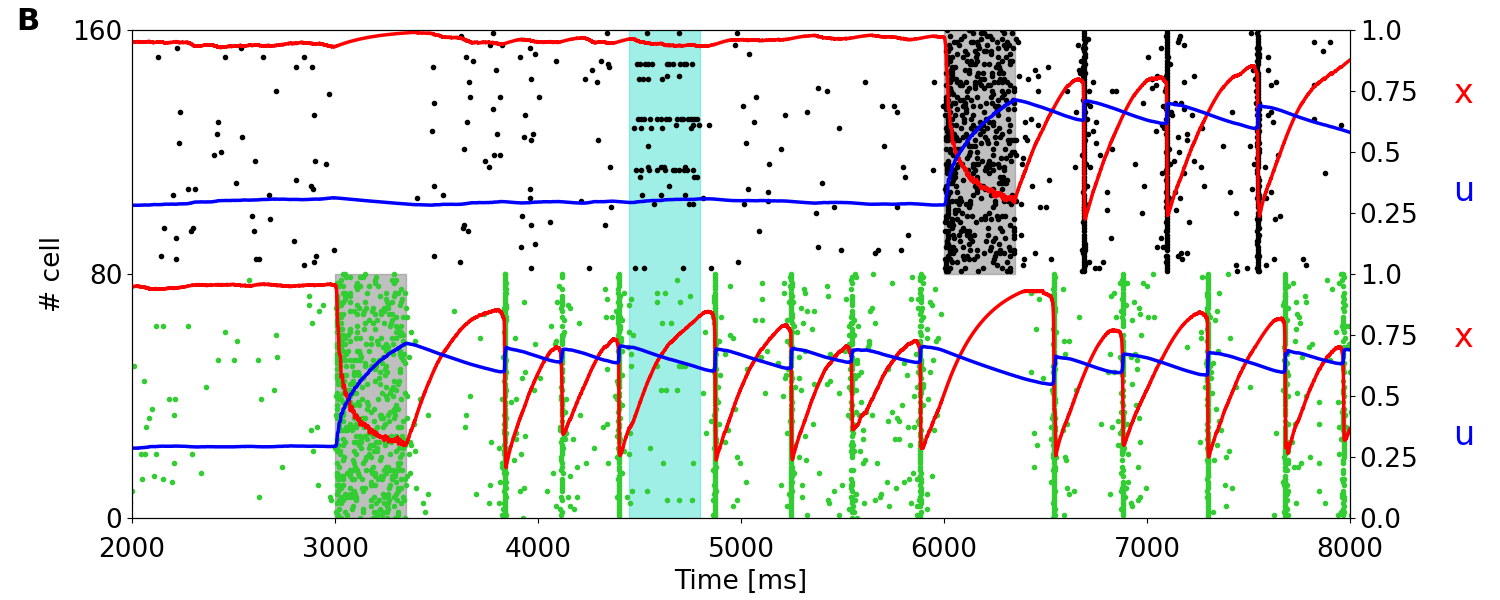
\includegraphics[width=0.9\columnwidth]{figures/fig3B.png}
    \caption{Raster plots of a subset of neurons of two targeted selective populations when two items are loaded into the network. An additional noise (cyan shading), which targets the 15\% of the excitatory neurons, is injected to test the network's robustness. \textbf{(A)} Network showing a single stable activity state injected with a periodic readout signal targeting all the excitatory neurons. After the second memory is loaded into the network, the populations show alternating population spikes. \textbf{(B)} Network in the bi-stable regime showing synchronous spiking activity. Here the network does not receive the periodic input since the synchronous activity autonomously shows up after the item loading. After the second memory is loaded the population spikes of the stimulated selective populations alternates, refreshing the synaptic variables in order to maintain the synchronous spiking activity. Figure from \cite{Tiddia2022_WM}.}
    \label{fig:figure3}
\end{figure}


The behavior of the network in Figure \ref{fig:figure3} is totally comparable with respect to the results shown in \cite{Mongillo2008}. The main differences that emerge are related, as stated before, to the dynamics of the STP variable $x$ which shows a more pronounced drop when neurons show synchronous firing activity. We slightly increased the time interval between two consecutive stimulations in Figure \ref{fig:figure3}A, from $250$\,ms to $300$\,ms, to make the STP variable $x$ recover enough to enable the synchronous activity response as in Figure \ref{fig:figure2}A. Shorter time intervals between subsequent readout signals could result in stimulation that lead to a population spike right after the end of the stimulus.

\begin{figure}[H]
    \centering
    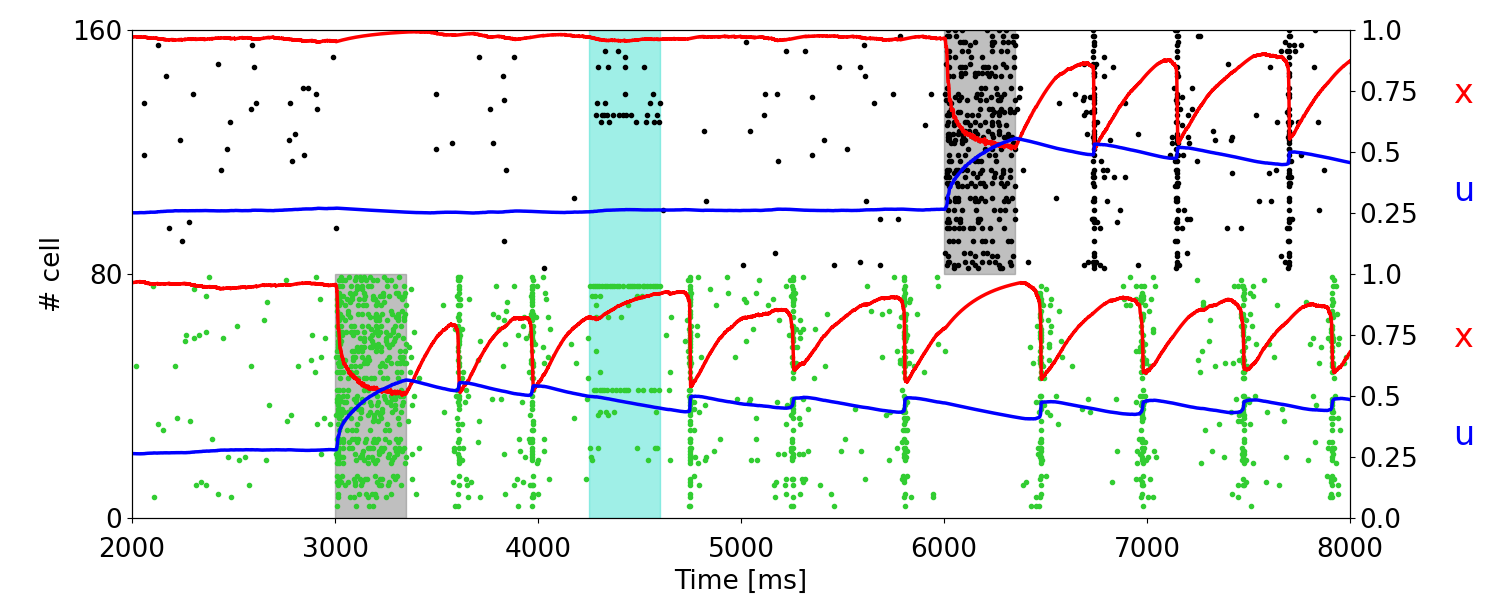
\includegraphics[width=0.9\columnwidth]{figures/fig5.png}
    \caption{Raster plot for a simulation with overlapping populations. Here only a subset of the two targeted selective populations is shown. An additional noise (cyan shading) is also injected. The network is in the bi-stable regime showing synchronous spiking activity. Figure from \cite{Tiddia2022_WM}.}
    \label{fig:figure5}
\end{figure}

Hitherto we presented the results of the simulations for the model with non-overlapping populations, ergo an excitatory neuron can only belong to a selective population at most. To verify the network's behavior in more realistic conditions we also performed simulations in which there is the possibility of having overlaps between the selective populations. In Figure \ref{fig:figure5} is shown the raster plot of a simulation with the same parameters used in Figure \ref{fig:figure3}B, but with overlapping populations. 


Here, the population spikes are less synchronized and not all the neurons belonging to the selective population emit a spike during the synchronous spiking activity. For this reason, the STP variable $x$ drops caused by the population spikes are less pronounced. To obtain a qualitatively similar behavior with respect to the network with non overlapping populations the value of the potentiated synaptic efficacy $J_p$ has been slightly increased to $0.49$\,mV.


\subsubsection{Study on network's memory capacity}

In \cite{mi_katkov_tsodyks2017} (see also \cite{Taher2020} for a similar derivation) is provided an analytical expression to estimate the maximal number of items that can be maintained in a working memory model sustained by STP. This number is determined by the ratio between $T_{\text{max}}$, i.e. the maximal period of the limit cycle of the network, and $t_s$, i.e. the time interval between two successive population spikes. Indeed, the maximal period of the limit cycle is only dependent by STP parameters and can be expressed by \cite{mi_katkov_tsodyks2017}
\begin{equation}
    T_{\text{max}} \simeq \tau_d \ln \dfrac{\tau_f/\tau_d}{1-U}
    \label{eq:Tmax_WMCapacity}
\end{equation}

This equation is then validated in \cite{mi_katkov_tsodyks2017} by performing simulations using a spiking neural network with a similar structure to the one shown in \cite{Mongillo2008}, thus we decided to perform simulations similar to the one of \cite{mi_katkov_tsodyks2017} using our implementation and test the validity of Equation \eqref{eq:Tmax_WMCapacity}. To this aim, we perform simulations with additional item loading signals targeting other selective populations for the network state showing synchronous spiking activity (same value of background input as in Figure \ref{fig:figure2}B). We noticed that the network was able, using these parameters, to keep up to three items. The raster plot, together with the averaged STP variables for the three targeted selective populations, is depicted in Figure \ref{fig:figure4}.

\begin{figure}[h]
    \centering
    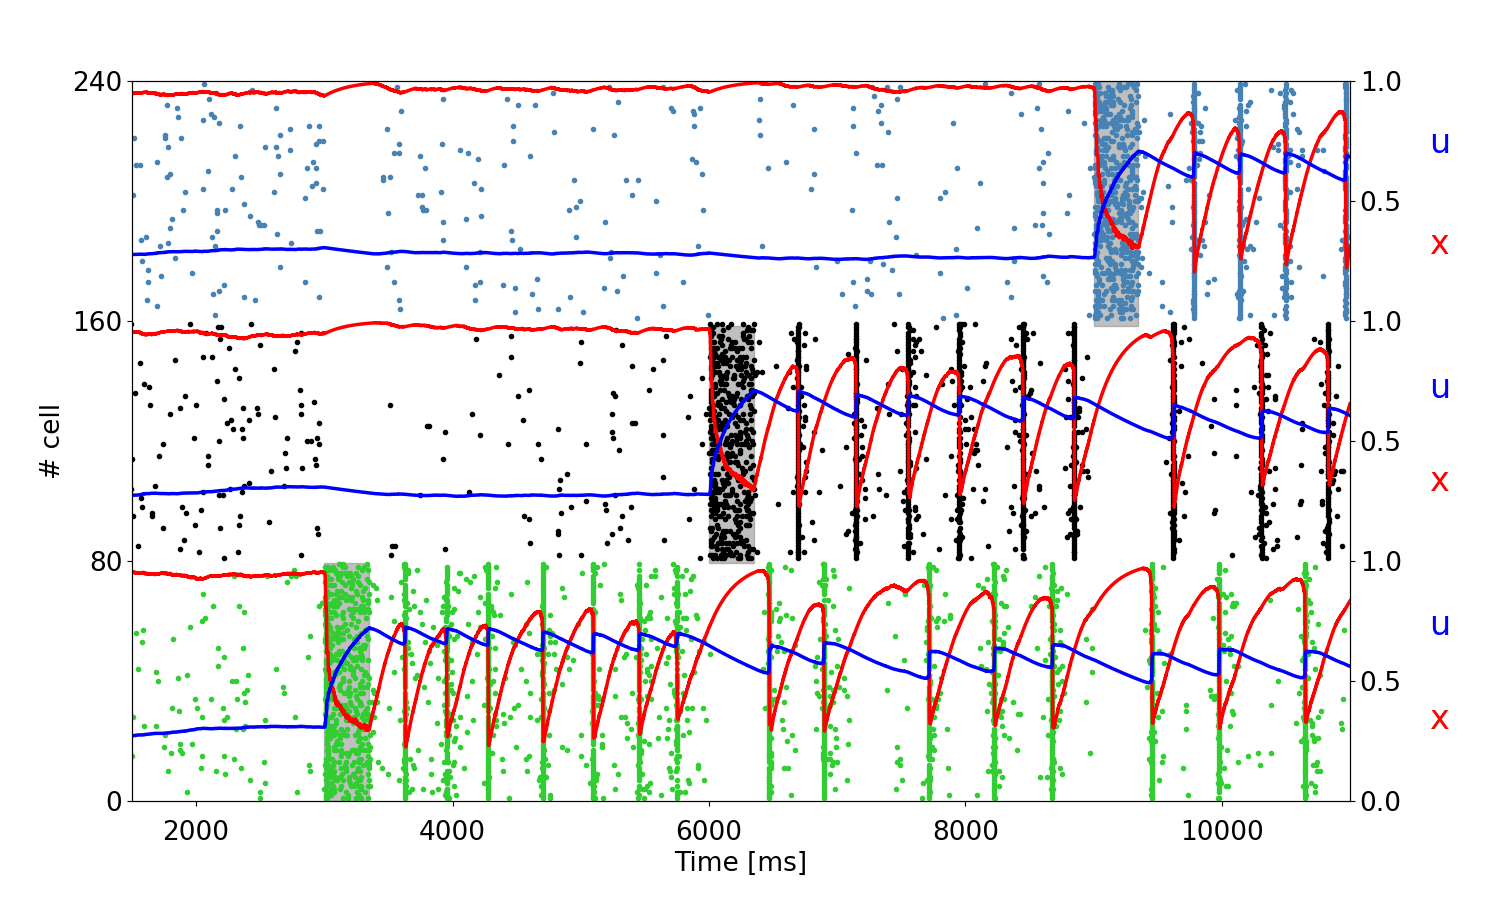
\includegraphics[width=0.9\columnwidth]{figures/fig4.png}
    \caption{Raster plot of a subset of neurons of three targeted selective populations when three items are loaded into the network. 
    The network is in the bi-stable regime showing synchronous spiking activity. Item stimuli are loaded into the network at $3000$, $6000$ and $9000$\,ms. Figure from \cite{Tiddia2022_WM}.}
    \label{fig:figure4}
\end{figure}


As shown in Figure \ref{fig:figure4}, the network is able to maintain three selective populations in the persistent activity state similarly to Figure \ref{fig:figure3}B so that, when all the items are loaded, population spikes alternate within the population keeping appropriate values for the STP variable. Moreover, it should be noted that each selective population in the synchronous spiking activity regime diminishes the average value for the STP variable $u$ when other items are loaded into the network. This behavior is clearly visible for the first selective population of Figure \ref{fig:figure4}. Indeed, this is due to the increased distance between population spikes related to the activity of the other targeted selective populations. For an increasing number of items loaded, this can lead to a loss of synchronicity, since persistent activity state needs relatively high values of $u$ to be maintained.


Using the parameters employed to produce Figure \ref{fig:figure4}, in which up to three items can be stored, $T_{\text{max}}\simeq 445$\,ms, whereas the time separation between the population spike, once the three items have been loaded into the network, is approximately $t_s \simeq 160$\,ms, with the ratio between these times being $$N_c\approx T_{\text{max}}/t_s\simeq 2.8$$ not far from the number of items stored at the same time, confirming the generality of the analytical estimation proposed in \cite{mi_katkov_tsodyks2017}.


We also performed a similar calculation for a network able to store more items. To do so, an increase in the value of $\tau_f$ is needed to enhance facilitation, thus enabling the upkeep of more items. Moreover, we decided to increase the network size. The default network model has 10000 LIF neurons and has a total of $p=5$ selective populations. Since in \cite{mi_katkov_tsodyks2017} a network of 20000 LIF neurons and ten selective populations is described, we decided to use similar parameters to perform simulations with a larger network having a higher number of selective populations. To do so, we chose $f=0.4$, $p=10$, $N_{\text{E}}=16000$, $N_{\text{I}}=4000$, $J_b = 0.05$ (as in \cite{mi_katkov_tsodyks2017}). A simulation with a single item loaded was performed to tune the external background input targeting the excitatory neurons in order to show synchronous spiking activity. We found that $\mu_{\text{ext}}=26.5$\,mV was able to show the desired behavior. We simulated the network using different values of $\tau_f$ to notice the change in the number of items which can be simultaneously maintained, and we observed a similar behavior discussed with the smaller network, so a higher value of $\tau_f$ is needed to keep a larger number of items in memory. In particular we observed that with $\tau_f = 4000$\,ms, $\tau_d = 250$\,ms seven memories can be loaded into the network at the same time. The raster plot of the selective populations in this configuration of the model is shown in Figure \ref{fig:rasterplot_7}.

\begin{figure}[h]
    \centering
    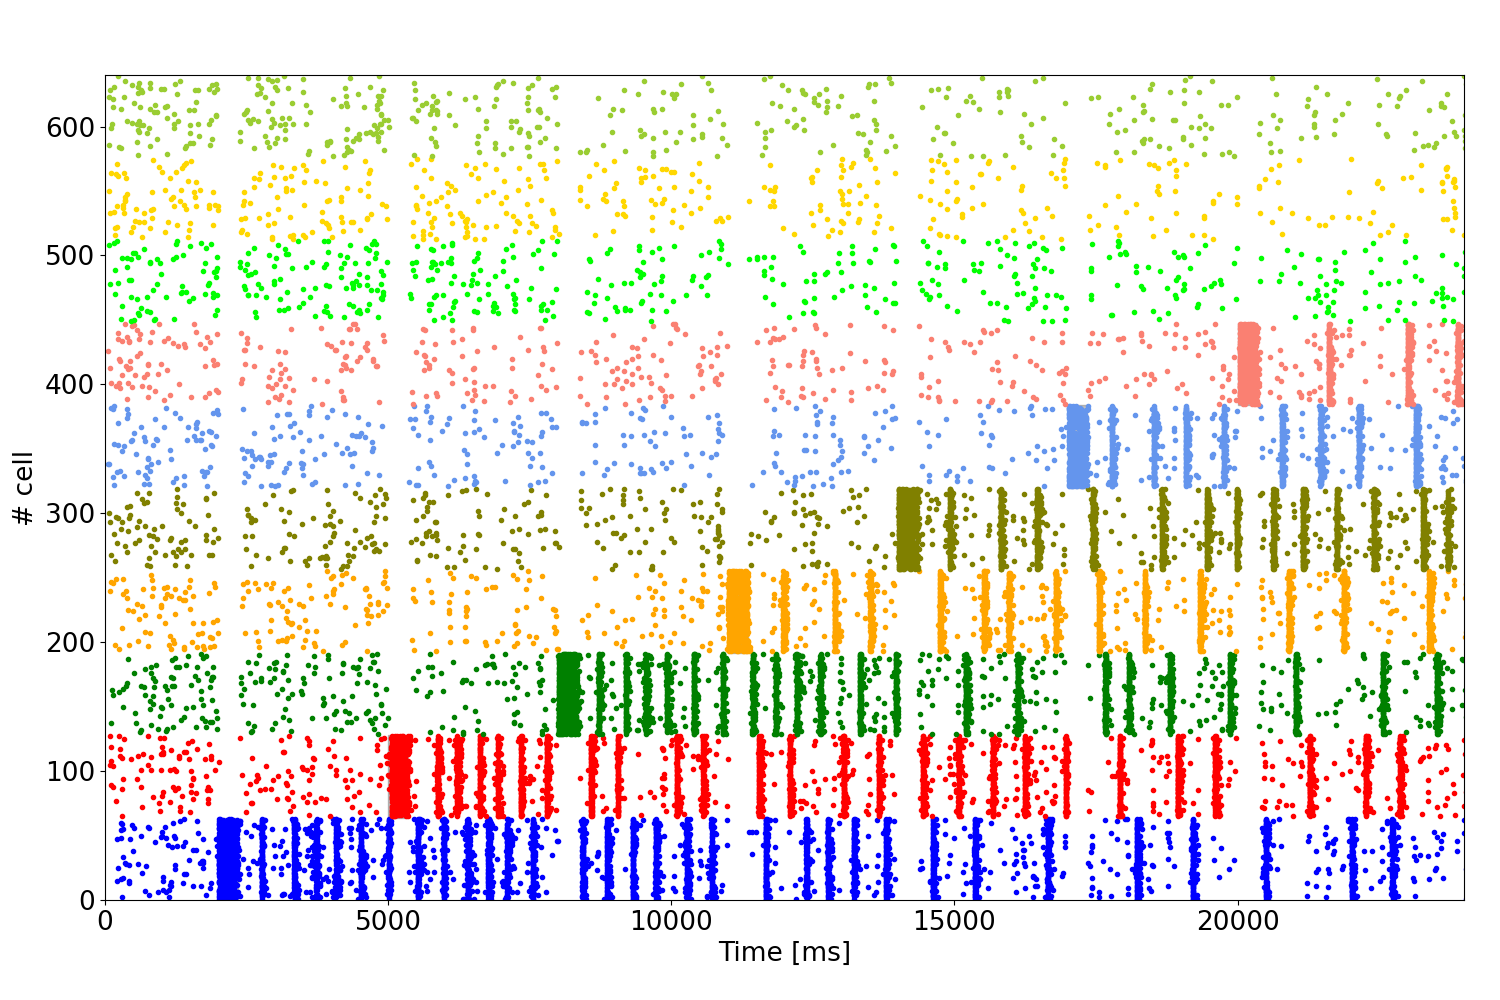
\includegraphics[width=0.9\columnwidth]{figures/raster_plot_7_items.png}
    \caption{Raster plot of a subset of the ten selective populations of the model. An item loading signal is injected every $3000$\,ms for each of the first seven selective populations starting from $2000$\,ms. The network, simulated using $\tau_f=4000$\,ms, $\tau_d=250$\,ms, is able to maintain seven targeted selective populations in the synchronous activity state. Figure from \cite{Tiddia2022_WM}.}
    \label{fig:rasterplot_7}
\end{figure}

Regarding the theoretical estimation of the working memory capacity, using the parameters employed to obtain Figure \ref{fig:rasterplot_7}, we estimate that the maximal period of the limit cycle of the network is $T_{max}\simeq 745$\,ms, whereas the time between two successive population spikes after having loaded all the seven items is $t_s=140(40)$\,ms. Those values lead to an analytical estimation of working memory capacity between $4.1$ and $7.5$, with the average estimation being equal to $5.3$, which is slightly smaller than the effective number of items kept in memory. However, it is still compatible with it considering the large uncertainty in this estimation.


\section{Discussion of the results}
\label{sec:WM_STP_discussion}

In this chapter we have shown the results of the working memory spiking network model proposed by \cite{Mongillo2008} reproduced in \cite{Tiddia2022_WM} using NEST and following the network description and the parameters shown in the original work. However, we have not limited to a reproduction of the model, and we explore the flexibility of the STP-driven mechanism through several tests.


Indeed, the spiking network model proposed here has some differences with respect to the original one of \cite{Mongillo2008}. First, we employed a LIF neuron model with exponential postsynaptic currents, whereas in the original one is used a LIF model with instantaneous rise and decay times for postsynaptic currents. Furthermore, the neuron model is integrated following the exact integration method of \cite{Rotter1999}, with synaptic variables for the neuron $i$ synapses updated when the neuron $i$ emits a spike, as mentioned in the Results section. The implementation of the STP dynamics follows Equations \eqref{eq:STP} and \eqref{eq:tsodyks3}. The implementation of the STP dynamics further differs with respect to the original work. In fact, in \cite{Mongillo2008} and \cite{mi_katkov_tsodyks2017} the absolute synaptic efficacy is modulated using the values of the variables $u$ and $x$ immediately before the emission of the spikes. As described in Equation \eqref{eq:tsodyks3}, the implementation used in this work considers the value of the variable $x$ immediately before the spike emission, but with the variable $u$ updated at the time of the emission of the spike, in agreement with \cite{tsodyks1998}. This change in the implementation leads to higher modulated synaptic efficacies for the implementation employed in this work (see also \cite{Gast2021} for a comparison of the two different implementations in a network of QIF neurons), and thus can be responsible for the more pronounced drop of the variable $x$ noticed in the spiking model presented in this work. Despite these differences, we were able to obtain a similar behavior with respect to the original model by slightly adjusting some parameters. However, other parameters were missing, like the integration time step, which we to set at $0.05$\,ms, verifying that lower or higher time steps do not entail significant changes in the network behavior. Moreover, the connection scheme in the NEST simulator opens to the possibility of having multiple connections with the same two neurons or also self connections. We thus checked that enabling or disabling this possibility does not change significantly the spiking activity, maintaining the same qualitative results to the one shown in this chapter. Furthermore, we also performed simulations with the same neuron model integrated with a different integration scheme with respect to the exact integration method of \cite{Rotter1999}. Specifically, we employed the stochastic Runge-Kutta method, more suitable in the presence of noise signals modeled as the background input employed in this network. We found that the results of the simulations are totally comparable with respect to the one presented here. The results of these studies are shown in Appendix \ref{app:wm_additional_tests}.

Figure \ref{fig:figure2}, showing the raster plot of a selective population targeted by an item loading signal and a non-targeted population, exhibits totally comparable results with respect to the original work, showing that the network can operate at relatively low firing rate and with modest (or even negligible) increase in firing rate during the delay period. These results are consistent with several experimental observations. For instance, in \cite{Wolff2015, Wolff2017} it is shown that, during the delay period, the information held in memory can be reactivated by a non-specific stimulus (as in Figure \ref{fig:figure2}A). This result is also shown by \cite{Rose2016}, in which transcranial magnetic stimulation produced a brief reactivation of the held item. Moreover, the silent dynamics can lead to interference between information from different trials \cite{Kilpatrick2018}, and the relation between STP dynamics and the so-called serial effects in WM tasks has recently been explored in \cite{Kiyonaga2017} and \cite{Barbosa2020}. Furthermore, the firing rate changes between the spontaneous state and the delay period shown in the right panels of Figure \ref{fig:figure2} are in agreement with single-cell firing rate, which are mostly below $5$\,Hz and only rarely can reach values greater than $10$\,Hz \cite{Shafi2007}. Indeed, since a higher spiking activity would be more metabolically demanding, this behavior makes the model energetically efficient underlining the importance of an activity-silent dynamics during working memory tasks, as suggested in \cite{Attwell2001} and \cite{Lennie2003}.

On the other hand, this model has some limitations, the main one being that it assumes a prior long-term Hebbian learning. The way items are encoded in selective populations is extremely simplified, as all the connections within the same population have equal synaptic strength. Furthermore, this value remains constant during the simulation. A more realistic model would be a combination of long-term and short-term plasticity, enabling the learning of new items.


In conclusion, to provide a qualitative comparison of the results, this chapter shows simulation protocols and raster plots totally similar to the ones of the original work. Indeed, the original work does not provide the code or the data of the spiking activity of the network, thus only a qualitative comparison was possible. The work of \cite{Tiddia2022_WM} has reproduced the results, with the aim of providing the simulation code and the data needed for further studies oriented towards a better understanding of working memory mechanisms and the link between short-term synaptic plasticity and long-term cognitive processes such as learning\footnote{The implementation of the model and the analysis code can be found at \url{https://github.com/gmtiddia/working_memory_spiking_network}.}.


Indeed, more studies on this model have been performed during my research stay at Institute of Neuroscience and Medicine (INM-6) of the Jülich Research Center, in the group of Computational Neurophysics under the supervision of Dr. Tom Tetzlaff. These studies are focused on a direct comparison based on specific test protocols between working memory mechanisms sustained by attractor network dynamics or synaptic mechanisms such as STP. These tests are oriented towards the applicability of such a mechanisms in hierarchical network models performing sequence learning. In \cite{Bouhadjar2022} it is shown a spiking model able to reproduce the temporal-memory part of the Hierarchical Temporal Memory (HTM) algorithm of \cite{hawkins2011cortical}, which is able to learn sequences of inputs, making predictions and autonomously replay the sequence. In order for this model to assume a hierarchical structure and being able to encode sequences of sequences, a further mechanism is needed to keep a sequence in memory for a longer time. Thus, I worked on the possible implementation of the STP-driven working memory mechanism in such a model. However, such a project is still ongoing with some preliminary results, so I decided do not report them in the main body of this thesis. Some of the preliminary results are reported in Appendix \ref{app:wm_additional_tests}.




\chapter{\textbf{Learning through structural plasticity: a theoretical framework}}
\label{chapter:structural_plasticity_theory}

\begin{tcolorbox}[colback=white,colframe=DarkRed,title=\textbf{Summary}]
This chapter presents the framework for learning with structural plasticity described also in \cite{Tiddia2023}. The chapter focuses in particular on the description of the theoretical framework and all the options that can be chosen to include some important features. In the first part of the chapter, a feed-forward network model is discusses, with the last part focusing on an extension of the latter provided with recurrent connections and additional neuron populations.
\end{tcolorbox}

\section{Model introduction}
As described in Section \ref{sec:str_pl_and_learning}, it is commonly believed that learning is influences not only by a change of synaptic efficacy of existing synapses, but also the change in the connection structure of neural circuits have a relevant role. In recent years, several computational models for structural plasticity were developed showing intriguing results regarding the relation of this mechanism in learning and other cognitive processes.\\
Here we want to propose a novel model for learning through a mechanism of structural plasticity. 
Since the biochemical and biophysical mechanisms underlying structural plasticity are extremely complex and only partially understood to date, this model exploits a relatively simple phenomenological model, including both the activity-driven and the homeostatic contributions according to what discussed in Section \ref{sec:str_pl_and_learning}. 
Despite the lower complexity, this model accounts for the effects of structural plasticity in terms of the consolidation of synaptic connections between neurons with a high activity correlation as well as those of pruning and rewiring the connections for which this correlation is lower. This approach is also justified by the requirement for a simple and effective computational model suitable for simulating networks with a relatively large number of neurons and connections and for representing learning processes with sizable numbers of training and validation patterns.


This model serves as the foundation for the creation of a mean-field-based theoretical framework for learning through synaptic plasticity capable of accounting for a variety of biological network properties. This framework is used in a training and validation procedure to characterize learning and memory capacity of plastic neuronal networks as the number of training patterns and other model parameters vary.
The proposed approach is capable of accounting for different probabilistic connection rules, firing rate probability distributions, presence of noise in stimuli, thus providing a general framework to study the impact of structural plasticity in learning on large-scale neuronal network models. Next section introduces the theoretical framework and how we implemented structural plasticity.

\section{Two neuron populations model}
Here we present the general model of two neuron populations connected feed-forwardly, and then the theoretical framework is divided into two possible approaches: a simple, discrete rate model in which neurons can only assume two possible firing rates values and a more realistic continuous rate model in which firing rates follow a continuous probability distribution. The following framework has been discussed in \cite{Tiddia2023}, and the following description entirely refers to this work.


The neuronal network model consists of two neuron populations, $\popI$ and $\popII$, of $10^5$ neurons each. This number corresponds roughly to the number of neurons in $1 \text{ mm}^2$ of cerebral cortex. The exchange of information between the two populations takes place through the connections from the population $\popI$ to the population $\popII$ (i.e. in a feed-forward fashion), which in the model are on average $5\cdot 10^3 $ per neuron of $\popII$, for a total of $5\cdot 10^8 $ connections. Each connection has an initial synaptic weight of $\Wb$. The first population ($\popI$) receives an input stimulus (e.g., visual) mimicked by the activation of the neurons with a firing rate pattern associated to it.


During the training stage, in addition to the signal from $\popI$, the second population receives another stimulus (e.g., auditory), that we identify as a \textit{contextual stimulus}. Figure \ref{fig:net_scheme} depicts a simple scheme of the network. 
Structural plasticity is modelled following the categories described in Section \ref{sec:str_pl_and_learning} and \cite{Fauth2016}, i.e., activity-dependent and homeostatic. The firing rate patterns of the two populations have a role in the activity-dependent structural plasticity.
The consolidation of a synaptic connection occurs when the firing rates of both the presynaptic and the postsynaptic neurons are concurrently above a certain threshold.
The synaptic weight of a consolidated connection increases from $\Wb$ to a value $\Wc > \Wb$. This is an effect of LTP, according to which we have the formation of new synapses, but also the growth of dendritic spines that increases synaptic efficacy of already existing synapses. Thus, the mechanism of consolidation proposed here embraces both structural and functional synaptic modifications. We flank this mechanism with synaptic rewiring, introduced later in this chapter. Once a synaptic connection has been consolidated, it will maintain the synaptic weight $\Wc$, without the possibility of returning to the initial state $\Wb$. This approach is a computationally-effective way of representing the biological structural changes that make a consolidated connection strong and durable. 

The sets of input and contextual patterns used for network training are independent firing-rate patterns of the two populations randomly generated from predefined firing rate probability distributions, which can be either discrete or continuous. The training process is performed using $\T$ independent input patterns, together with the corresponding contextual stimuli. A diagram of the training and validation processes is shown in Figure \ref{fig:net_scheme}. During training, when both input and contextual stimulus are used, a fraction of the neurons in the population $\popII$ will assume a rate above threshold.
These neurons, called {\it coding}, or {\it selective} neurons, play a vital role in input coding. The existence of neurons showing selective firing rate in response to specific stimuli is largely confirmed by experimental results. The average input signal to these neurons will be called $\langle \SII \rangle$. The non-selective neurons of $\popII$ will instead be called {\it non-coding} or {\it background} neurons, and their average input signal will be indicated with $\langle \Sb \rangle$. The proposed model accounts for the ability of the network to learn the association between input patterns and the corresponding contextual stimuli.


\begin{figure}[H]
\centering
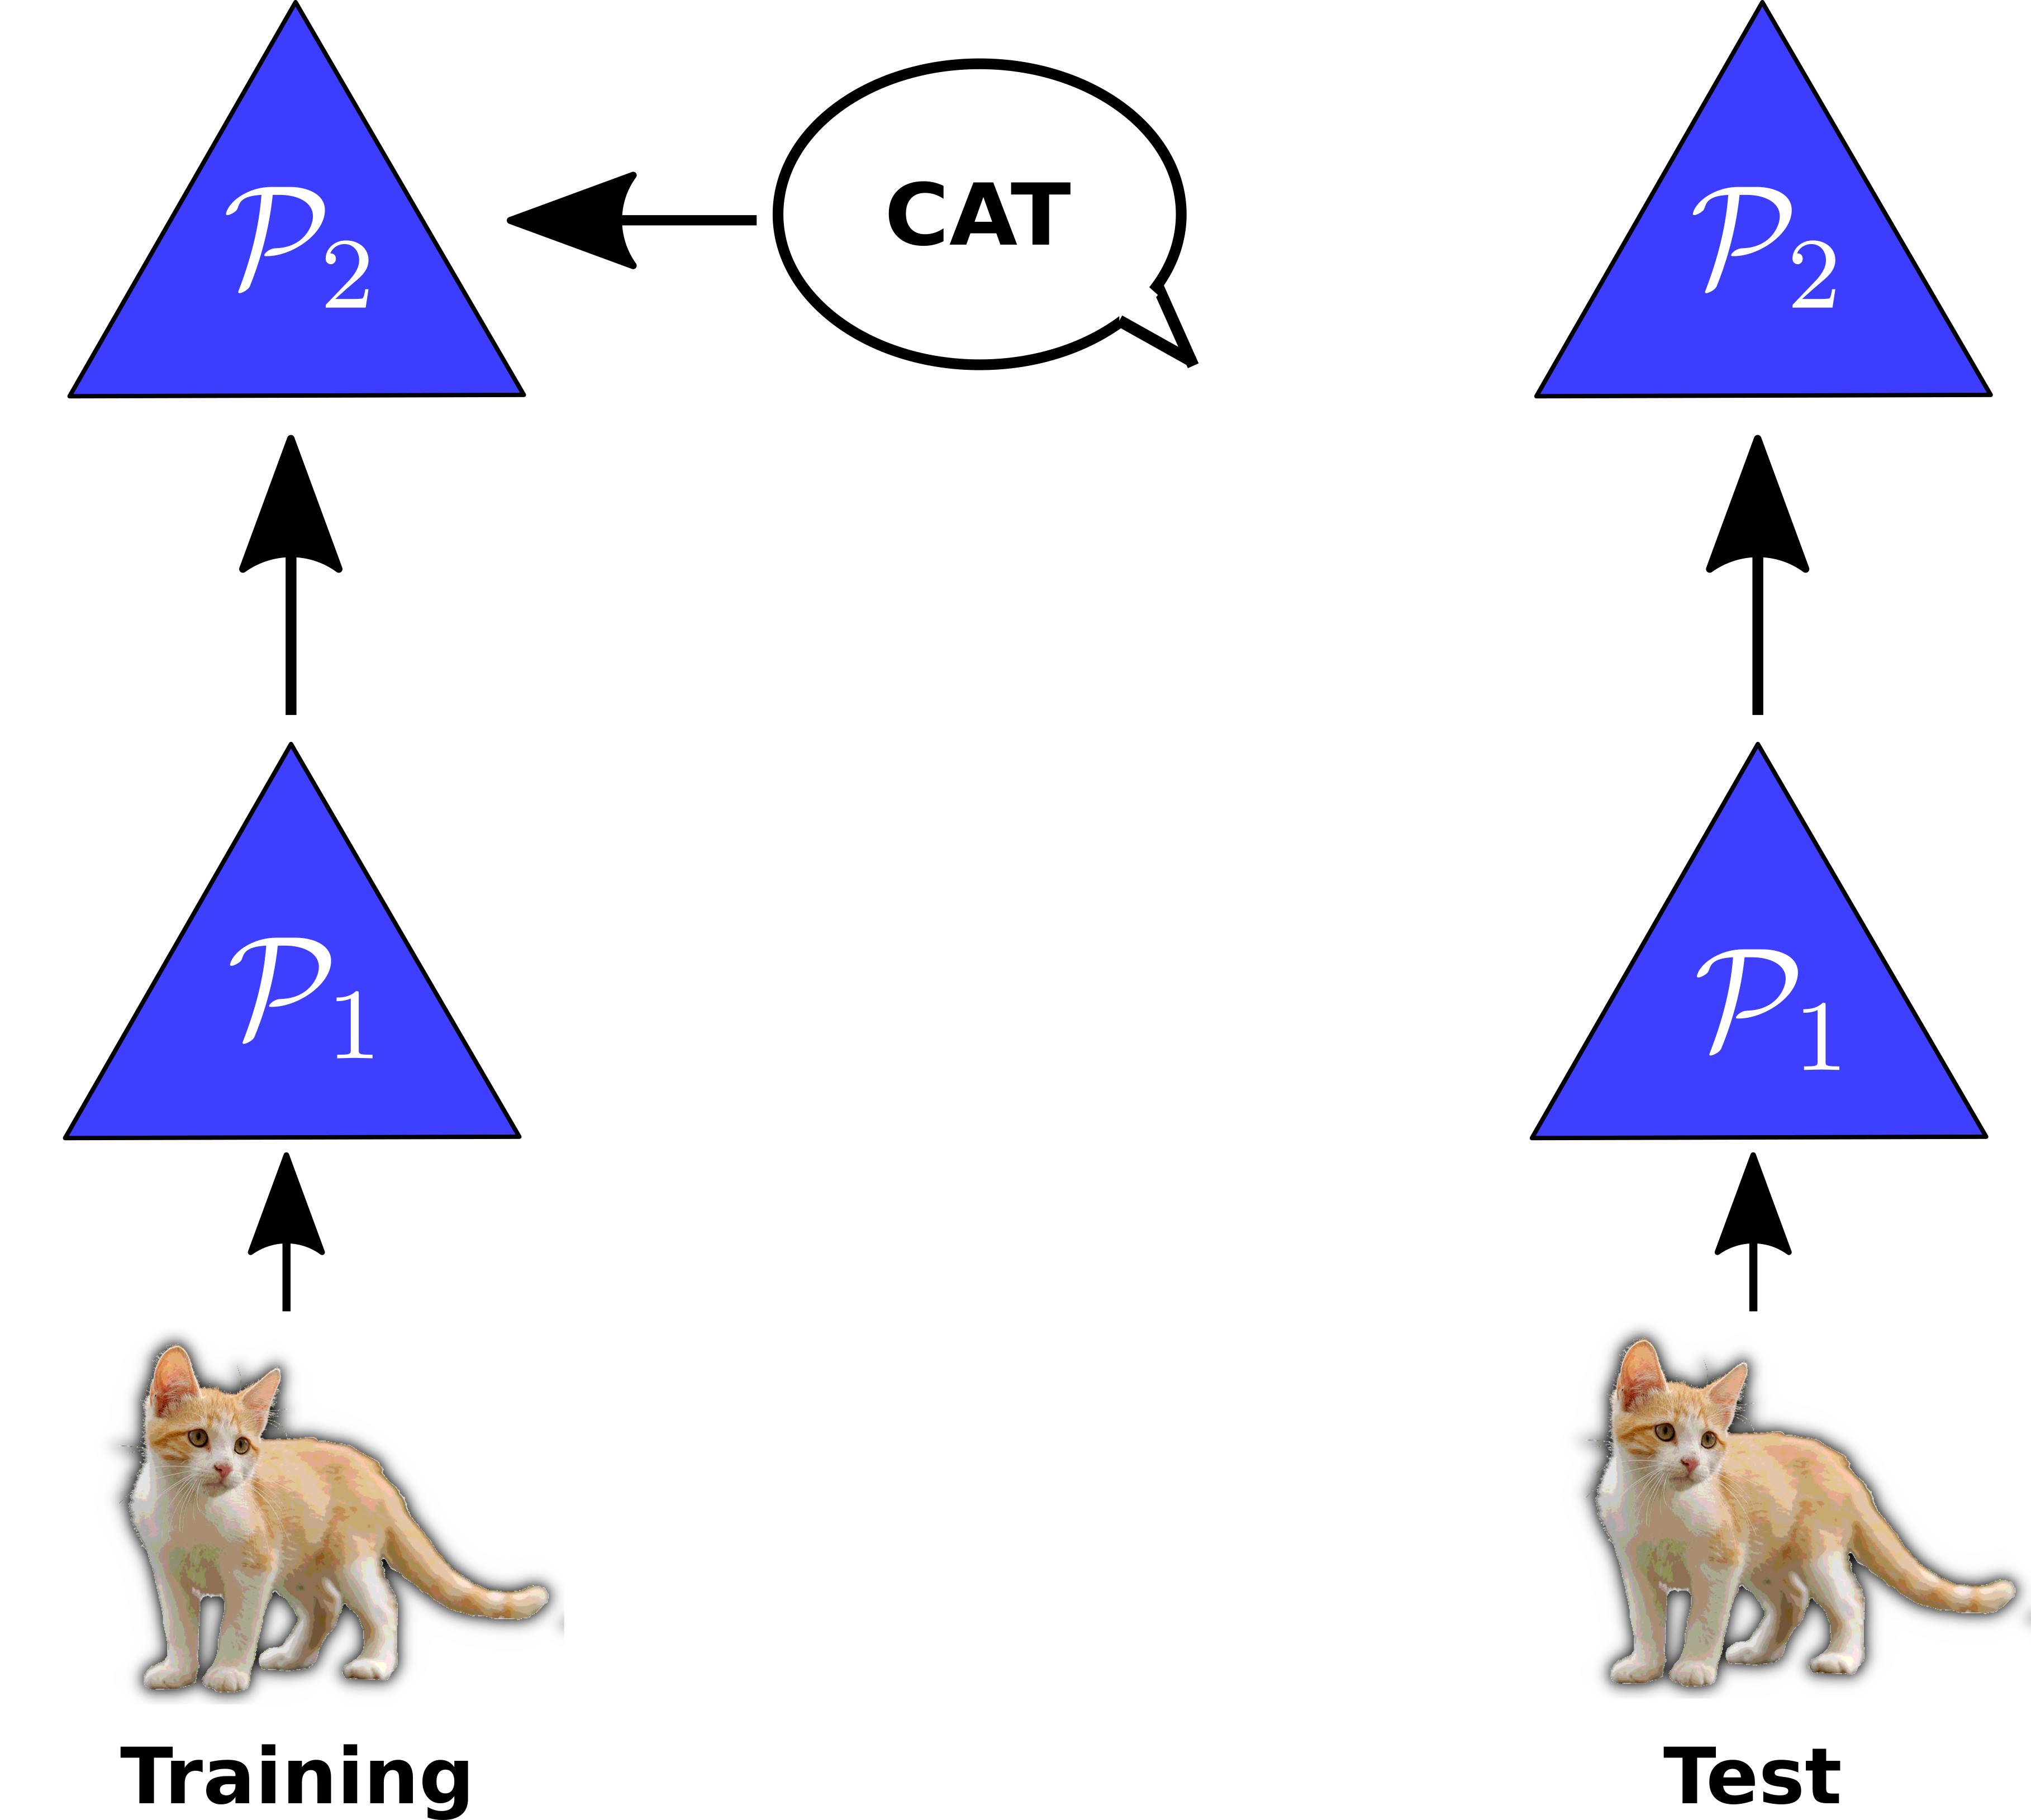
\includegraphics[scale=0.85]{figures/str_pl.png}
\caption{Schematic representation of the network model through a block diagram. During training (left), a visual stimulus is injected into $\popI$ and an auditory stimulus is injected into $\popII$ as contextual stimulus.
In test phase (right) one of the visual patterns is injected without the corresponding contextual stimulus. The cat image is adapted from \href{https://commons.wikimedia.org/wiki/File:Golden\_tabby\_and\_white\_kitten\_n01.jpg}{Golden tabby and white kitten} by Marie-Lan Nguyen / Wikimedia Commons / CC-BY 2.5. Figure from \cite{Tiddia2023}.}
\label{fig:net_scheme}
\end{figure}

We may distinguish two different types of models based on the potential values that the neuron firing rate can assume:
\begin{itemize}
     \item \textbf{Discrete model}, in which neurons rate can assume only two discrete values $\rl$ (low rate) and $\rh$ (high rate);
     \item \textbf{Continuous model}, in which neurons rate follow a continuous probability distribution (here lognormal).
\end{itemize}
In the next section we will derive the mean-field equations for these two models, which are summarized in the following tables.

\renewcommand{\arraystretch}{1.2}

\begin{table}[H]
%%%%%%%%%%%%%%%%%%%
\begin{tabular}{
  |@{\hspace*{\marg}}p{0.2\textwidth}@{\hspace*{\marg}}
  |@{\hspace*{\marg}}p{0.8\textwidth}@{\hspace*{\marg}}
  |}
  \hline 
  \multicolumn{2}{|>{\color{white}\columncolor{black}}c|}{\textbf{Summary}}\\
  %\multicolumn{2}{|c|}{\cellcolor[HTML]{000000}{\color[HTML]{FFFFFF} \textbf{Summary}}}\\
  \hline 
  \textbf{Populations} & $\popI$, $\popII$ \\
  \hline 
  \textbf{Connectivity} & sparse random connectivity\\
  \hline 
  \textbf{Neurons} & firing-rate-based models of point-like neurons
  \\
  \hline 
  \textbf{Synapses} & structural plasticity \\
  \hline 
  \textbf{Input} & firing rate pattern extracted from a discrete or continuous probability distribution  \\
  \hline 
\end{tabular}
\begin{tabular}{
  |@{\hspace*{\marg}}p{0.2\textwidth}@{\hspace*{\marg}}
  |@{\hspace*{\marg}}p{0.4\textwidth}@{\hspace*{0.0pt}}
  |@{\hspace*{\marg}}p{0.4\textwidth}@{\hspace*{0.0pt}}
  |}
  \hline 
  \multicolumn{3}{|>{\color{white}\columncolor{black}}c|}{\textbf{Populations}}\\
  \hline 
  \textbf{Name} & \textbf{Elements} & \textbf{Size}\\
  \hline 
  $\popI$  & point-like neurons & $\NI$\\
  \hline 
  $\popII$  & point-like neurons & $\NII$\\
  \hline 
\end{tabular}
\begin{tabular}{
  |@{\hspace*{\marg}}p{0.2\textwidth}@{\hspace*{\marg}}
  |@{\hspace*{\marg}}p{0.8\textwidth}@{\hspace*{\marg}}
  |}
  \hline 
  \multicolumn{2}{|>{\color{white}\columncolor{black}}c|}{\textbf{Neuron }}\\
  \hline 
  \textbf{Type} & firing-rate-based neuron model\\
  \hline 
  \textbf{Firing rate distribution} & 
    \begin{itemize}
    \item discrete model: the firing rates can assume only two discrete values $\rh$ (high rate) and $\rl$ (low rate);
    \item continuous model: the firing rates can assume values from a continuous probability distribution (here lognormal).
    \end{itemize}\\
  \hline 
\end{tabular}
%%%%%%%%%%%%%%%%%%%

\begin{tabular}{
  |@{\hspace*{\marg}}p{0.2\textwidth}@{\hspace*{\marg}}
  |@{\hspace*{\marg}}p{0.8\textwidth}@{\hspace*{\marg}}
  |}
  \hline 

  \multicolumn{2}{|>{\color{white}\columncolor{black}}c|}{
  \textbf{Synapse}
  }\\
  \hline 
  \textbf{Type} & structural plasticity\\
  \hline 
  \textbf{Description} & initial synaptic weight are set to $\Wb$ for all the instantiated connections;
  when a training pattern is used, considering a connection between a $\popI$ neuron $i$ and a $\popII$ neuron $j$:
                         \begin{itemize}
                            \item (discrete model) $\Wb \rightarrow \Wc$ if $\nu_\text{i}=\nu_\text{j}=\rh$;
                            \item (continuous model) $\Wb \rightarrow \Wc$ if $\nu_\text{i}>\rtI$ and $\nu_\text{j}>\rtII$.
                         \end{itemize}
                        Once a connection is consolidated, it cannot return to the initial weight.
  \\
  \hline 
\end{tabular}

%%%%%%%%%%%%%%%%%%% 
\caption{Description of the network model (continues on next page).}
\label{tab:model_description}
\end{table}
\addtocounter{table}{-1}
\begin{table}[H]
%%%%%%%%%%%%%%%%%%%
%%%%%%%%%%%%%%%%%%%
\begin{tabular}{
  |@{\hspace*{\marg}}p{0.1\textwidth}@{\hspace*{\marg}}
  |@{\hspace*{\marg}}p{0.1\textwidth}@{\hspace*{0.0pt}}
  |@{\hspace*{\marg}}p{0.8\textwidth}@{\hspace*{0.0pt}}
  |}
  \hline 
  \multicolumn{3}{|>{\color{white}\columncolor{black}}c|}{
  \textbf{Connectivity}
  }\\
  \hline 
  \textbf{Source} & \textbf{Target} & \textbf{Pattern}\\
  \hline
  $\popI$ & $\popII$ & %
                      \begin{itemize}
                      \item random, independent; in-degrees can be homogeneous, with a fixed number of $\C$ connections per neuron of $\popII$, or driven by a Poisson distribution;
                      \item synaptic weights are $\Wb$ for unconsolidated connections and $\Wc$ for consolidated ones, with $\Wc>\Wb$;
                      \item multiple connections between the same couple of presinaptic and postsinaptic neurons (``multapses'') are allowed by default, but they can be disabled.
                      \end{itemize}\\
  % \hline
  % all & all & no self-connections (``autapses''), multiple connections (``multapses'') are permitted\\
  \hline

\end{tabular}
%%%%%%%%%%%%%%%%%%%
\begin{tabular}{
  |@{\hspace*{\marg}}p{0.2\textwidth}@{\hspace*{\marg}}
  |@{\hspace*{\marg}}p{0.8\textwidth}@{\hspace*{\marg}}
  |}
  \hline 

  \multicolumn{2}{|>{\color{white}\columncolor{black}}c|}{
  \textbf{Connection rewiring}
  }\\
  \hline 
  \textbf{Description} & periodically, unconsolidated connections are pruned, and new connections are created: if $h$ is the number of consolidated incoming connections of a neuron of $\popII$, $\C - h$ new connections will be created, were $\C$ is a fixed number if the fixed-indegree connection rule is used, while it is extracted from a Poisson distribution if the Poisson-indegree rule is selected; in both cases, the presynaptic neurons are randomly extracted from $\popI$.
  \\
  \hline 
\end{tabular}
%%%%%%%%%%%%%%%%%%%
\begin{tabular}{
  |@{\hspace*{\marg}}p{0.2\textwidth}@{\hspace*{\marg}}
  |@{\hspace*{\marg}}p{0.8\textwidth}@{\hspace*{\marg}}
  |}
  \hline 
  \multicolumn{2}{|>{\color{white}\columncolor{black}}c|}{
  \textbf{Input stimulus}
  }\\
\hline 
\textbf{Description} & firing rate pattern of the neurons of $\popI$ selected from the training or from the test set.\\
\hline 
\end{tabular}
%%%%%%%%%%%%%%%%%%%
\begin{tabular}{
  |@{\hspace*{\marg}}p{0.2\textwidth}@{\hspace*{\marg}}
  |@{\hspace*{\marg}}p{0.8\textwidth}@{\hspace*{\marg}}
  |}
  \hline 
  \multicolumn{2}{|>{\color{white}\columncolor{black}}c|}{
  \textbf{Contextual stimulus}
  }\\
\hline 
\textbf{Description} & firing rate pattern of the neurons of $\popII$ selected from the training set; used only in the training phase.\\
\hline 
\end{tabular}
%%%%%%%%%%%%%%%
\begin{tabular}{
  |@{\hspace*{\marg}}p{0.2\textwidth}@{\hspace*{\marg}}
  |@{\hspace*{\marg}}p{0.8\textwidth}@{\hspace*{\marg}}
  |}
  \hline 
  \multicolumn{2}{|>{\color{white}\columncolor{black}}c|}{
  \textbf{Train set}
  }\\
\hline 
\textbf{Type} & set of $T$ independent firing-rate patterns of the neurons of $\popI$ (input stimulus) and $\popII$ (contextual stimulus). \\
\hline 
  \textbf{Description} &
  each pattern is randomly generated from predefined firing rate probability distributions, which can be discrete or continuous:
    \begin{itemize}
    \item discrete model: the firing rates can assume only two discrete values $\rh$ (high rate) and $\rl$ (low rate) with probabilities $p_1$ and $q_1 = 1 - p_1$ in the $\popI$ population, $p_2$ and $q_2 = 1 - p_2$ in the $\popII$ population.  
    \item continuous model: the firing rates can assume values on the basis of a continuous probability distribution; this work uses a lognormal distribution.
    \end{itemize}\\
\hline
\end{tabular}
\caption{Description of the network model (continues on next page).}
\end{table}
\addtocounter{table}{-1}
\begin{table}[H]
\begin{tabular}{
  |@{\hspace*{\marg}}p{0.2\textwidth}@{\hspace*{\marg}}
  |@{\hspace*{\marg}}p{0.8\textwidth}@{\hspace*{\marg}}
  |}
  \hline 
  \multicolumn{2}{|>{\color{white}\columncolor{black}}c|}{
  \textbf{Test set}
  }\\
\hline 
\textbf{Type} & set of $V$ firing-rate patterns of the neurons of $\popI$ (input stimulus) \\
\hline 
  \textbf{Description} &
  each pattern is randomly extracted from the train set and eventually altered by adding noise from a predefined distribution:
    \begin{itemize}
    \item discrete model: the pattern is left unchanged;
    \item continuous model: the firing rate of each neuron is modified by adding a random deviation extracted from a predefined probability distribution; in this work we used a truncated Gaussian distribution. 
    \end{itemize}\\
\hline
\end{tabular}
%%%%%%%%%%%%%%%%%%%
\caption{Description of the network model (continues on next page).}
\end{table}

\def\widthA{0.1}
\def\widthB{0.25}
\def\widthC{0.65}
\begin{table}[H]
  \begin{tabular}{
    |@{\hspace*{\marg}}p{\widthA\textwidth}@{\hspace*{\marg}}
    |@{\hspace*{\marg}}p{\widthB\textwidth}@{\hspace*{\marg}}
    |@{\hspace*{\marg}}p{\widthC\textwidth}@{\hspace*{\marg}}
    |}
    \hline 
    \multicolumn{3}{|>{\columncolor{black}}c|}{\color[HTML]{FFFFFF} \textbf{Network and connectivity}}\\
    \hline 
    \textbf{Name} & \textbf{Value } & \textbf{Description}\\
    \hline 
    $\NI$ & $100000$ & number of neurons of $\popI$\\
    \hline 
    $\NII$ & $100000$ & number of neurons of $\popII$\\
    \hline 
    $\C$ & $5000$ & number of connection in-degrees per neuron of $\popII$\\
    \hline 
    $\T$ & variable & number of training patterns\\
    \hline 
    $s$ & 100 & connection rewiring step\\
    \hline 
    \end{tabular}
  %%%%%%%%%%%%%%%%%%%%%%%%%%%%%%%%%%%%%%%%%%%%% 
  \begin{tabular}{
    |@{\hspace*{\marg}}p{\widthA\textwidth}@{\hspace*{\marg}}
    |@{\hspace*{\marg}}p{\widthB\textwidth}@{\hspace*{\marg}}
    |@{\hspace*{\marg}}p{\widthC\textwidth}@{\hspace*{\marg}}
    |}
    \hline
    \multicolumn{3}{|>{\columncolor{black}}c|}{
    \textbf{\color[HTML]{FFFFFF} Neuron}
    }\\
    \hline 
    \textbf{Name} & \textbf{Value } & \textbf{Description}\\
    \hline 
    $\rl$ & $2.0\sps$ & low firing rate\\
    \hline 
    $\rh$ & $50\sps$ & high firing rate\\
    \hline 
    \end{tabular}
  %%%%%%%%%%%%%%%%%%%%%%%%%%%%%%%%%%%%%%%%%%%%% 
  \begin{tabular}{
    |@{\hspace*{\marg}}p{\widthA\textwidth}@{\hspace*{\marg}}
    |@{\hspace*{\marg}}p{\widthB\textwidth}@{\hspace*{\marg}}
    |@{\hspace*{\marg}}p{\widthC\textwidth}@{\hspace*{\marg}}
    |}
    \hline
    \multicolumn{3}{|>{\columncolor{black}}c|}{\color[HTML]{FFFFFF} 
    \textbf{Synapse}
    }\\
    \hline 
    \textbf{Name} & \textbf{Value } & \textbf{Description}\\
    %%%%%%%%%%%%%%%%%%%%
    %% transmission
    \hline
    $\Wb$ & $0.1$\,pA & baseline synaptic weight\\
    \hline
    $\Wc$ & $1$\,pA & consolidated synaptic weight \\
    \hline
    \end{tabular}
  %%%%%%%%%%%%%%%%%%%%%%%%%%%%%%%%%%%%%%%%%%%%% 
  \begin{tabular}{
    |@{\hspace*{\marg}}p{\widthA\textwidth}@{\hspace*{\marg}}
    |@{\hspace*{\marg}}p{\widthB\textwidth}@{\hspace*{\marg}}
    |@{\hspace*{\marg}}p{\widthC\textwidth}@{\hspace*{\marg}}
    |}
    \hline
    \multicolumn{3}{|>{\columncolor{black}}c|}{\color[HTML]{FFFFFF} 
    \textbf{Stimulus}
    }\\
    \hline 
    \textbf{Name} & \textbf{Value } & \textbf{Description}\\
    %%%%%%%%%%%%%%%%%%%%
    %% transmission
    \hline
    $p_1$ & $0.001$ & probability for a neuron of $\popI$ of having high rate when an input stimulus is injected\\
    \hline
    $p_2$ & $0.001$ & probability for a neuron of $\popII$ of having high rate when a contextual stimulus is injected \\
    \hline
  \end{tabular}
  \caption{Model parameters.}
  \label{tab:model_parameters}
\end{table}

\subsection{\label{subsubseq:rate-discr} Discrete rate model}
As previously mentioned, in this model the input and contextual stimuli are represented by discrete firing-rate patterns of the two populations, $\popI$ and $\popII$ respectively, in which the firing rate of each neuron can assume only two possible values, $\rh$ (high rate) or $\rl$ (low rate). Each training example consists of two patterns, one representing the input stimulus to the population $\popI$,
the other representing the contextual stimulus to the population $\popII$. The pattern representing the input stimulus is generated by randomly extracting the firing rate of each neuron of $\popI$ from the two values, $\rh$ and $\rl$, with probabilities $p_1$ and $q_1 = 1-p_1$, respectively. The corresponding pattern for the contextual stimulus is generated in a similar way, extracting the values of the firing rates of the $\popII$ neurons, $\rh$ or $\rl$, with probabilities $p_2$ and
$q_2 = 1-p_2$, respectively.
The mean number of high-rate neurons in the two populations will be:
\begin{equation}
\label{eq:Nh}
\begin{split}
     N_{h,1}&=\NI p_1 \\
     N_{h,2}&=\NII p_2
     \end{split}
\end{equation}
where $\NI$ and $\NII$ indicate the number of neurons of $\popI$ and $\popII$, respectively.
A connection will be consolidated in a training example if both the presynaptic and the postsynaptic neuron assume a high firing rate $\rh$.
The probability that a generic connection is consolidated in a single example is $p_1 p_2$, and thus the probability that it is not consolidated after $\T$ training examples is
$(1-p_1p_2)^{\T}$.
The probability $p$ that a connection is consolidated in at least one of the $\T$ training examples is given by the complement of the previous expression:
\begin{equation}
\label{eq:p}
     p= 1-(1-p_1 p_2)^\T
\end{equation}
The product of this expression by the number of incoming connections per neuron $\C$ gives us the average number of consolidated connections per neuron:
\begin{equation}
\label{eq:av_k}
     \langle k \rangle=\C \Bigl[ 1 - (1-p_1p_2)^{\T} \Bigr] = \C p
\end{equation}
For each neuron we will therefore have on average $\langle k \rangle$ consolidated connections with synaptic weight $\Wc$ and $\C- \langle k \rangle$ unconsolidated connections with synaptic weight $\Wb$.

The test set consists of $V$ firing-rate patterns of the neurons of $\popI$, randomly extracted from the $\T$ input patterns of the train set. In the discrete rate model, the pattern are unaltered, thus each input patter of the test set is identical to an input pattern of the train set.
The contextual stimuli are not used in the validation phase.

The average rate of the neurons in the population  $\popI$ is
\begin{equation}
\label{eq:av_r}
    \langle \nu \rangle = p_1\rh + (1-p_1)\rl
\end{equation}
The input signal targeting a non-coding neuron of $\popII$ (i.e., a background neuron) is equal to the weighted sum of the signals coming from the $\C$ connections:
\begin{equation}
\label{eq:Sb}
   \Sb = \Wc \sum_{i=1}^{ k}\nu_i +\Wb \sum_{i=1}^{\C- k } \xi_i
\end{equation}
where $\C$ is the number of incoming connections, $k$ is the number of consolidated connections, $\nu_i$ are the firing rates of the neurons connected to the consolidated connections and $\xi_i$ are the firing rates of the neurons connected to the unconsolidated connections.
From the linearity of $\Sb$ with respect to $\nu_i$ and $\xi_i$ and from the fact that the rates of presynaptic neurons have the same mean value $\langle \nu \rangle$, it follows that
\begin{equation}
\label{eq:av_sb}
    \langle \Sb \rangle = [ \Wc \langle k \rangle 
    +  \Wb (\C - \langle k \rangle) ] \langle \nu \rangle
\end{equation}
In this equation, we can clearly observe two distinct contributions: one related to consolidated connections, which depends on the mean value $\langle k \rangle$, and the other related to unconsolidated connections, which depends on $\C - \langle k \rangle$.
From this result we can now calculate the variance on the background signal, which is defined as:
\begin{equation}
     \sigma_{b}^{2}=\langle (\Sb-\langle \Sb \rangle)^2 \rangle
\end{equation}
Using Equations \eqref{eq:Sb} and \eqref{eq:av_sb}, we can compute the variance as:
\begin{equation}\label{eq:discrprelim}
    \sigma_{b}^{2}= \langle \Bigl[ \Wc \sum_{i=1}^{k}\nu_i +\Wb \sum_{i=1}^{\C-k} \xi_i 
    - [ \Wc \langle k \rangle 
    +  \Wb (\C - \langle k \rangle) ] \langle \nu \rangle \Bigr]^2 \rangle
\end{equation}
Taking advantage of the equality $\langle k \rangle=k+(\langle k \rangle-k)$, we can rewrite:
\begin{equation}
   \Wc \langle k \rangle
    + \Wb (\C - \langle k \rangle)
    = \Wc k + \Wc (\langle k \rangle - k) + \Wb \Bigl[(\C-k) + (k-\langle k \rangle ) \Bigr] =
\end{equation}
\begin{equation*}
     =\Wc k + \Wb (\C- k) + \Wc (\langle k \rangle - k)  + \Wb (k - \langle k \rangle)
\end{equation*}
Inserting this last expression in Equation \eqref{eq:discrprelim} and rewriting the terms with the multiplicative factors $k$ and $\C - k$ with summations, such as for example $\Wc k \langle \nu \rangle = \Wc \sum_{i=1}^{k} \langle \nu \rangle$, we obtain:
\begin{equation}
\label{eq:var_sb2}
     \sigma_{b}^2 = \langle \Bigl[ \Wc \sum_{i=1}^k (\nu_i - \langle \nu \rangle) +\Wb \sum_{i=1}^ {\C-k} (\xi_i - \langle \nu \rangle) + (k-\langle k \rangle)(\Wc-\Wb)\langle \nu \rangle \Bigr]^2 \rangle
\end{equation}
Taking into account that the mixed terms go to zero since $\sum_{i} \langle(x_i - \langle x \rangle) \rangle=0$, setting $\sum_{i} (x_i - \langle x \rangle)^ 2=\sigma^{2}_{x}$, we will have that:
\begin{equation}
\label{variance_sigmab}
     \sigma_{b}^2= \Bigl[\Wc^2 \langle k \rangle + \Wb^2 (\C - \langle k \rangle)\Bigr] \sigma_{\nu}^2 + (\Wc - \Wb)^2 \sigma_{k}^2 \langle \nu \rangle ^2
\end{equation}
where $\sigma_{k}^2 = \langle (k- \langle k\rangle )^2 \rangle$.
In the previous formula we note two contributions depending respectively on the variance of the firing rate and on the variance of the number of consolidated connections.
The value of the variance of $k$ is not shown here, but is derived in Appendix \ref{app:var_k}, whereas the variance of the rate is, by definition, $\sigma^2_{\nu}=\langle\nu^2\rangle - \langle\nu\rangle^2$. \\
Now we estimate the average input to a coding neuron of $\popII$. The neuron receives signals from neurons of $\popI$ coming from both consolidated and unconsolidated connections.
If $\C$ is the number of incoming connections, the average number of high-rate presynaptic neurons will be $p_1 \C$, while those with low rate will be on average $\C' = \C (1 - p_1)$.
Since the input pattern used for validation is identical to the corresponding training pattern, the $p_1 \C$ connections coming from high rate neurons will certainly be consolidated.
The remaining $\C'$ connections come from neurons of $\popI$ at low rate, however they may have been consolidated in other training examples.
The average number of consolidated connections
from low-rate neurons can be calculated using Equation \eqref{eq:av_k}:
\begin{equation}
\label{eq:av_k1}
    \langle k' \rangle = \C' p = \C(1-p_1) p = \langle k \rangle (1 - p_1)
\end{equation}

For a better understanding, the following scheme represents an example of coding and non coding neurons during test phase. 

\begin{figure}[H]
    \centering
    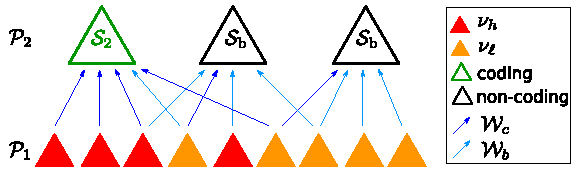
\includegraphics[width=\columnwidth]{figures/test_str_pl.pdf}
    \caption{Scheme of a subset of the network during test phase. Red and amber triangles represent single neurons of $\popI$ having high or low rate, respectively. Dark and light blue arrows represent consolidated and unconsolidated connections, whereas green and black triangles represent coding or non-coding neuron of $\popII$.}
    \label{fig:test_str_pl}
\end{figure}

As we can see, a coding neuron receives, from high rate neurons of $\popI$ only consolidated connections, but it can have consolidated or unconsolidated connections from low rate neurons. Summing up all the contributions, the average value of $\SII$ is

\begin{equation}
\label{eq:s2}
\begin{split}
    \langle \SII \rangle &= \Wc \C p_1 \rh + \Wc \langle k' \rangle \rl + \Wb (\C' - \langle k' \rangle) \rl =\\
    &= \Wc \C p_1 \rh + \Wc \langle k \rangle (1-p_1) \rl + \Wb (\C - \langle k \rangle) (1-p_1) \rl =\\
    &= \Wc \C p_1 \rh + \Bigl[ (\Wc - \Wb) \langle k \rangle + \C \Wb  \Bigr] (1-p_1)\rl
\end{split}
\end{equation}

The previous formula does not consider the rewiring of the connections; the effect of rewiring will be described in Section \ref{subseq:rewiring}, where we will derive the expression of $\SII$ that takes it into account.
We identify this case as "with rewiring" to distinguish it from the case in which unconsolidated connections are not pruned and rewired. Indeed, this distinction is useful to estimate the contribution of this mechanism on the input signal on coding neurons of $\popII$.

Now, it is possible to obtain the signal-difference-to-noise-ratio (SDNR) using the formula
\begin{equation}
\label{eq:SDNR}
    \text{SDNR} = \dfrac{|\langle \SII \rangle - \langle \Sb \rangle |}{\sigma_b}
\end{equation}

Here the SDNR is calculated on the input signal to the coding and non-coding neurons of the $\popII$ population due to the connections coming from the $\popII$ population, rather than on the firing rates of the $\popII$ neurons.
This choice is justified by the need to evaluate the memory capacity associated with the plasticity of the connections from $\popI$ to $\popII$.
In general, in addition to the signal from the $\popI$ population, the $\popII$ neurons will receive other excitatory and inhibitory signals in input.
As described in Section \ref{sec:firing_rate_models}, in rate-based models, the response of neurons to the overall input signal is generally described by an activation function that expresses the firing rate as a function of that signal.
A common choice is the threshold-linear (or ReLU) function described also in Equation \eqref{eq:ReLu}:

\begin{equation}
\Phi(x) = \alpha \text{max}\{ 0, x\}
\end{equation}

where $\alpha$ is a multiplicative coefficient. With this choice,
the average rates of coding and non-coding neurons of $\popII$ can be written as

\begin{equation}
\begin{split}
\langle\nu_\text{c}\rangle &=
    \Phi(\langle\SII\rangle + \langle S_\text{o}\rangle - S_\text{thresh}) \\
\langle\nu_\text{nc}\rangle &=
    \Phi(\langle\Sb\rangle + \langle S_\text{o}\rangle - S_\text{thresh})
\end {split}
\end{equation}

where $\langle S_\text{o}\rangle$ is the average input signal from (excitatory and/or inhibitory) neuron populations
different from $\popI$ and $S_\text{thresh}$ is the activation threshold.
Assuming that the total input signal is above the threshold for both coding and non-coding neurons, the average rates will be linear functions of the input signals:

\begin{equation}
\begin{split}
\langle\nu_\text{c}\rangle &=
    \alpha(\langle\SII\rangle + \langle S_\text{o}\rangle - S_\text{thresh}) \\
\langle\nu_\text{nc}\rangle &=
    \alpha(\langle\Sb\rangle + \langle S_\text{o}\rangle - S_\text{thresh})
\end {split}
\end{equation}

while the variance of the non-coding neuron rate will be

\begin{equation}
\sigma_\text{nc}^2 = \alpha^2 (\sigma_\text{b}^2 + \sigma_\text{o}^2)
\end{equation}

The SDNR calculated on the rate will therefore be

\begin{equation}
\label{eq:SDNRnu}
    \text{SDNR}_\nu = 
    \dfrac{|\langle\nu_\text{c}\rangle - \langle\nu_\text{nc}\rangle|}
    {\sigma_\text{nc}} =
        \dfrac{|\langle \SII \rangle - \langle \Sb \rangle |}
        {\sqrt{\sigma_\text{b}^2 + \sigma_\text{o}^2}}
\end{equation}

which has an expression similar to that reported in Equation \eqref{eq:SDNR}, with the only difference that there is an additional contribution to the noise due to the signal coming from other populations.

Note also that the definitions of SDNR reported in Equations \eqref{eq:SDNR} and \eqref{eq:SDNRnu} refer to the mean signal difference between single coding and non-coding neurons. However, the overall memory capacity of the synaptic connections between the two populations can be best quantified by the SDNR evaluated on the total input signal to coding neurons and to an equivalent number of non-coding neurons.
Calling $N_{h,2}$ the mean number of coding neurons in the population $\popII$, we can define

\begin{equation}
\label{eq:SDNRpop}
\text{SDNR}_\text{pop} = 
    \dfrac{|
    N_{h,2}
    \langle \SII \rangle - N_{h,2}
    \langle \Sb \rangle |}
        {\sqrt{N_{h,2}}
        \sigma_\text{b}} =
    \dfrac{\sqrt{p_2 \NII}
    |\langle \SII \rangle -
    \langle \Sb \rangle |}
        {\sigma_\text{b}}
\end{equation}

where we used Equation \eqref{eq:Nh} and $\sqrt{N_{h,2}}\sigma_\text{b}$ is the standard deviation of the total input signal to $N_{h,2}$ non-coding neurons.
Thus, $\text{SDNR}_\text{pop}$ scales with the square root of $p_2 N_2$.

Table \ref{tab:discrete_model} summarizes the equations of the discrete rate model.

\begin{table}[H]
    \centering
    \renewcommand\arraystretch{1.5}
    \begin{tabular}{
  |@{\hspace*{\marg}}m{0.3\textwidth}@{\hspace*{\marg}}
  |@{\hspace*{\marg}}m{0.1\textwidth}@{\hspace*{\marg}}
  |@{\hspace*{\marg}}m{0.6\textwidth}@{\hspace*{\marg}}
  |}
  \hline 
  \multicolumn{3}{|>{\color{white}\columncolor{black}}c|}{
  \textbf{Discrete rate model}
  }\\
  \hline 
  \textbf{Name} & \textbf{Symbol} & \textbf{Equation}\\
  \hline
  Rate mean & $\langle \nu \rangle$ & $p_1\rh + (1-p_1)\rl$\\
    \hline
  Rate variance & $\sigma_{\nu}^2$ & $\Big( p_1\rh^2 + (1-p_1)\rl^2 \Big)-\Big(p_1\rh + (1-p_1)\rl\Big)^2$\\
  \hline
  Average background signal & $\langle \Sb \rangle$ & $\langle k \rangle \Wc \langle \nu \rangle + (\C - \langle k \rangle) \Wb \langle \nu \rangle$\\
  \hline
  Variance of background signal & $\varSb$ & $\Bigl[\Wc^2 \langle k \rangle + \Wb^2 (\C - \langle k \rangle)\Bigr] \sigma_{\nu}^2 + (\Wc - \Wb)^2 \sigma_{k}^2 \langle \nu \rangle ^2$\\
  \hline
  Average coding neuron signal (without rewiring) & $\langle \SII \rangle$ &$\Wc \C p_1 \rh + \Bigl[ (\Wc - \Wb) \langle k \rangle + \C \Wb  \Bigr] (1-p_1)\rl$\\
  \hline
\end{tabular}
    \caption{Summary of the equations for the discrete model.}
    \label{tab:discrete_model}
\end{table}


\subsection{\label{subsubseq:rate-cont} Continuous model}
In this model the firing rate patterns are generated from a continuous probability distribution, $\rho(\nu)$.
The distinction between high-rate and low-rate neurons
is based on two rate thresholds, $\rtI$ for the population $\popI$ and $\rtII$ for the population $\popII$. The values of these thresholds are related to the fraction of neurons above the threshold for the two populations, $p_1$ and $p_2$, respectively, by the equations:
\begin{equation}
    \begin{split}
    p_1 &= \int_{\rtI}^{\infty} \rho (\nu) d\nu\\
    p_2 &= \int_{\rtII}^{\infty} \rho (\nu) d\nu\\
    \end{split}
\end{equation}
The average rates of the neurons of $\popI$ below and above threshold,
$\langle \rlI \rangle$ and $\langle \rhI \rangle$,
can be computed from the firing rate distribution as:
\begin{equation}
    \label{eq:av_rate_cont}
    \begin{split}
        \langle \rlI \rangle &= \int_{0}^{\rtI} \nu \rho (\nu) d\nu \Big/ \int_{0}^{\rtI} \rho (\nu) d\nu = \frac{1}{q_1}\int_{0}^{\rtI} \nu \rho (\nu) d\nu\\
        \langle \rhI \rangle &= \int_{\rtI}^{\infty} \nu \rho (\nu) d\nu \Big/ \int_{\rtI}^{\infty} \rho (\nu) d\nu = \frac{1}{p_1} \int_{\rtI}^{\infty} \nu \rho (\nu) d\nu
    \end{split}
\end{equation}
where $q_1 = 1- p_1$.
Similar equations can be used to compute
$\langle \rlII \rangle$ and $\langle \rhII \rangle$.
From these equations
the average firing rate of $\popII$ can be expressed as
\begin{equation}
    \langle \nu \rangle= 
    \int_{0}^{\infty} \nu \rho (\nu) d\nu
    = q_1 \langle \rlI \rangle + p_1 \langle \rhI \rangle 
    = q_2 \langle \rlII \rangle + p_2 \langle \rhII \rangle 
\end{equation}
In a training example, a connection will be consolidated if both the presynaptic and the postsynaptic neuron assume a firing rate above threshold.
Figure \ref{fig:lognormal} depicts an example of firing rate distribution, with the threshold and the average values of low and high firing rate. Adopting such a threshold mechanism, we are able to identify high and low rate neurons as in the discrete case, resembling thus the scheme shown in Figure \ref{fig:test_str_pl} for the discrete model during test phase. The only difference is that, since in this case the rate are not discrete, instead of having $\rh$ or $\rl$ we have $\langle \rh \rangle$ and $\langle \rl \rangle$.

\begin{figure}[t]
    \centering
    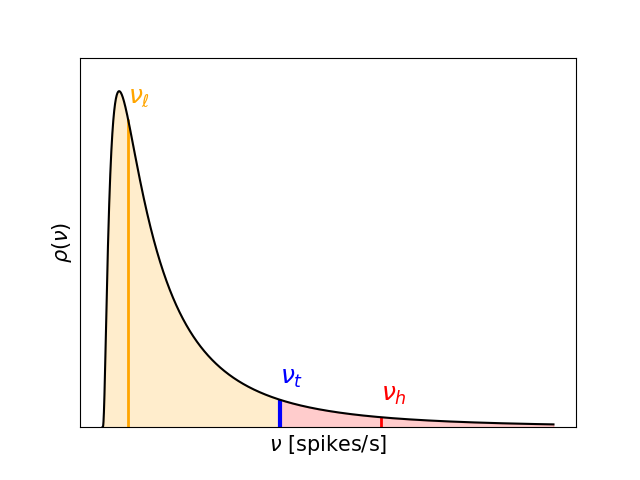
\includegraphics[scale=0.7]{figures/lognormal_dist.png}
    \caption{Lognormal distribution of firing rate. The black solid line indicates the probability distribution, which is divided into two sections by the rate threshold $\rt$ (blue, vertical line). The amber band represents the distribution of rate below the threshold, whose mean is $\rl$ (amber, vertical line). The red band represents the distribution of neurons whose rate is above threshold. Here the average of this section is $\rh$ (red, vertical line). Figure from \cite{Tiddia2023}.}
    \label{fig:lognormal}
\end{figure}

As in the discrete model, the test set consists of $V$ firing-rate patterns of the neurons of $\popI$, randomly extracted from the $\T$ input patterns of the train set.
Here we consider the case where the patterns are unchanged, thus each input patter of the test set is identical to an input pattern of the train set. In a later section we will discuss the effect of altering these patterns by adding noise.
To estimate the values of $\langle\SII\rangle$, $\langle\Sb\rangle$ and $\varSb$ we proceed in a similar way as for the discrete model.
First of all, we calculate the input signal to a generic non-coding neuron of $\popII$.
Let $\C$ be the number of incoming connections to this neuron,
$P(k)$ the probability that $k$ of these connections are consolidated, $\nu_1, \dotsi, \nu_k$ the firing rates of the
presynaptic neurons of the consolidated connections
and $\xi_1, \dotsi, \xi_{\C - k}$ the firing rates of the
presynaptic neurons of the unconsolidated connections.
The probability of having $k$ consolidated connections and rates in the range $(\nu_1, \nu_1+d\nu_1), \dotsi, (\nu_k, \nu_k + d\nu_k)$, $(\xi_1, \xi_1+d\xi_1), \dotsi, (\xi_{\C-k}, \xi_{\C-k} + d\xi_{\C-k})$ is $P(k)\rho (\nu_1)\dotsi \rho (\nu_k) \rho (\xi_1) \dotsi \rho (\xi_{\C-k})
d\nu_1 \dotsi d\nu_k d\xi_1 \dotsi d\xi_{\C-k}$.
To calculate the average background signal we should average the expression of $\Sb$, given by Equation \eqref{eq:Sb}, over all the possible values of $k$ and of the firing rates, thus 
\begin{equation}
\label{eq:av_sb_cont}
\begin{split}
    \langle \Sb \rangle &= \sum_{k} P(k) \int d\nu_1 \dotsi \int d\nu_k \int d\xi_1 \dotsi \int d\xi_{\C - k} \rho (\nu_1) \dotsi \rho (\nu_k) \rho (\xi_1) \dotsi \rho (\xi_{\C - k}) \cdot \\
    &\cdot\Bigl[ \Wc (\nu_1 + \dotsi + \nu_k) + \Wb (\xi_1 + \dotsi + \xi_{\C-k})\Bigr] = \\
    &= \sum_{k} P(k) \Bigl[ \Wc k \langle \nu \rangle + \Wb (\C-k) \langle \nu \rangle \Bigr]
    = [ \Wc \langle k \rangle 
    +  \Wb (\C - \langle k \rangle) ] \langle \nu \rangle
\end{split}
\end{equation}

where we used the fact that $\int \nu \rho(\nu) d\nu = \int \xi \rho(\xi) d\xi = \langle \nu \rangle$. Note that the result obtained in Equation \eqref{eq:av_sb_cont} is the same as the one obtained for the discrete model (see Equation \eqref{eq:av_sb}).

The variance of the background signal can be similarly derived:
\begin{equation}
\label{eq:var_sb_cont}
\begin{split}
    \varSb &=\langle(\Sb - \langle \Sb \rangle)^2\rangle = \sum_k P(k) \int d\nu_1  \dotsi \int d\nu_k \int d\xi_1 \dotsi \int d\xi_{\C-k} \rho(\nu_1) \dotsi \rho(\xi_{\C-k}) \cdot \\
    &\cdot \Bigl[ \Wc \sum_{i=1}^{k}\nu_i
    +\Wb \sum_{i=1}^{\C-k} \xi_i 
    - [ \Wc \langle k \rangle 
    +  \Wb (\C - \langle k \rangle) ] \langle \nu \rangle \Bigr]^2 = \\
    &= \sum_k P(k) \int d\nu_1 \dotsi \int d\xi_{\C-k} \rho(\nu_1) \dotsi \rho(\xi_{\C-k})
    \Bigl[ \Wc \sum_{i=1}^k (\nu_i - \langle \nu \rangle) +\Wb \sum_{i=1}^ {\C-k} (\xi_i - \langle \nu \rangle) + \\ 
    & + (k-\langle k \rangle)(\Wc-\Wb)\langle \nu \rangle \Bigr]^2
\end{split}
\end{equation}
    
Where in the last line we used the substitution $\langle k \rangle=k+(\langle k \rangle - k)$ as done for Equation \eqref{eq:var_sb2}.
The mixed terms of the equation above are null because $\int \rho (x) (x-\langle x \rangle)dx = 0$, ergo we can write the variance of the background signal as follows:

\begin{equation}
\label{eq:var_sb2_cont}
\begin{split}
    \varSb &= \sum_k P(k) \int d\nu_1 \dotsi \int d\xi_{\C-k} \rho(\nu_1) \dotsi \rho(\xi_{\C-k}) \Bigl[ \Wc^2 k \langle (\nu - \langle \nu \rangle)^2 \rangle + \Wb^2 (\C - k) \langle (\nu - \langle \nu \rangle)^2 \rangle +\\
    & + (\Wc - \Wb)^2 (k - \langle k \rangle)^2 \langle \nu \rangle ^2 \Bigr] = \Bigl[ \Wc^2 \langle k \rangle + \Wb^2 (\C - \langle k \rangle)\Bigr] \sigma_{\nu}^2 + (\Wc - \Wb)^2 \sigma_{k}^2 \langle \nu \rangle ^2
\end{split}
\end{equation}
The variance of $k$ has the same expression as for the discrete case, and is derived in  Appendix \ref{app:var_k}.
$\SII$ can be derived similarly to the discrete case as well.
We have a contribution from $p_1\C$ neurons of $\popI$ at high rate connected by consolidated connections.
The remaining $\C'= \C - p_1\C$ neurons have a low rate
and can be connected either by unconsolidated connections or by connections that have been consolidated in input patterns different from the current one.
Calling $\langle k' \rangle$ the average number of 
consolidated connections outgoing from the $\C'$ low-rate neurons and using the definition of $\langle \rl \rangle$ and $\langle \rh \rangle$ given by Equation \eqref{eq:av_rate_cont} we can write
\begin{equation}
\label{eq:s2_cont}
\begin{split}
    \langle \SII \rangle &= \Wc p_1 \C \langle \rh \rangle + (\Wc - \Wb) \langle k' \rangle \langle \rl \rangle + \Wb \C(1-p_1)\langle \rl \rangle =\\
    &= \Wc p_1 \C \langle \rh \rangle + \Bigl[ (\Wc - \Wb) \langle k \rangle + \C \Wb \Bigr] (1-p_1) \langle \rl \rangle
\end{split}
\end{equation}
where we used the expression of $\langle k' \rangle$
from Equation \eqref{eq:av_k1}.
As can be seen, Equation \eqref{eq:s2_cont} differs from \eqref{eq:s2} only because the rates are not discrete but can assume continuous values, thus the discrete values
$\rh$ and $\rl$ are replaced by the averages
$\langle \rh \rangle$ and $\langle \rl \rangle$.
The modified formula of $\SII$ that takes into account
connection rewiring will be derived in Section \ref{subseq:rewiring}.

In this work we use a lognormal distribution of the firing rates for the continuous model.
Indeed, it is known that rate distribution in the cortex are long-tailed and skewed with a lognormal shape 
\cite{Roxin2011}.
The lognormal distribution is a continuous probability distribution of a random variable $\nu$ whose logarithm 
$\ln(\nu)$ is normally distributed.
The probability density function of this distribution is
\begin{equation}
\label{eq:lognormal}
 \rho_\text{LN}(\nu) = \frac{1}{\sqrt{2\pi} \sigma \nu} \cdot \exp\Bigl( -\frac{(\ln(\nu)-\mu)^2}{2\sigma^2}\Bigr)
\end{equation}
where $\mu$ and $\sigma$ are the mean and standard deviation of $\ln(\nu)$.
The expressions of the mean value and standard deviation of $\rho_\text{LN}(\nu)$ will be derived in Appendix \ref{app:distr_fr}.

\subsubsection{\label{subsubseq:poiss-indegree} Poisson distribution of incoming connections per neuron}

Hitherto we considered a model in which each neuron of $\popII$ has a fixed number of incoming connections, i.e., a fixed in-degree, $\C$. However, a more general and more realistic approach would consider $\C$ as variable across the neurons of $\popII$
according to an appropriate probability distribution
$P(\C)$.
In this work we will focus on the case where the number of incoming connections follows a Poisson distribution (i.e. a Poisson-indegree connection rule), however the approach we will present can be easily extended to other distributions.
The values of $\langle \SII \rangle$ and $\langle \Sb \rangle$, previously averaged over the rate $\nu$ and the number of consolidated connections $k$, should be also averaged over the number of incoming connections, so that

\begin{equation}
    \begin{split}
        \langle \langle \Sb \rangle_{\nu,k} \rangle_{\C} &= \sum_{c} P(\C) \langle \Sb \rangle_{\nu,k}\\
        \langle \langle \SII \rangle_{\nu,k} \rangle_{\C} &= \sum_{\C} P(\C) \langle \SII \rangle _{\nu,k}
    \end{split}
    \label{eq:averaging_over_C}
\end{equation}

where $\langle \SII \rangle_{\nu,k}$ is given by Equation \eqref{eq:s2_cont} and $\langle \Sb \rangle _{\nu,k}$ is given by Equation \eqref{eq:av_sb_cont}. Since these equations are linear in $\C$ and since $\sum_{\C} \C P(\C) = \langle\C\rangle$, Equations \eqref{eq:s2_cont} and \eqref{eq:av_sb_cont} would show $\langle\C\rangle$ instead of $\C$ when averaged over the number of incoming connections per neuron.\\
The variance can be obtained from the equation: 
\begin{equation}
    \text{Var}(\langle \langle \Sb \rangle_{\nu,k}\rangle_{\C})= \sigma^2_{\nu,k,\C} =\langle\langle\Sb^2\rangle_{\nu,k}\rangle_{\C}-\langle\langle\Sb\rangle_{\nu,k}\rangle_{\C}^2
\end{equation}
Knowing that $\langle \varSb\rangle_{\C}=\langle \langle
\Sb^2\rangle_{\nu_k}-\langle\Sb\rangle_{\nu,k}^2\rangle_{\C}
=\langle\langle\Sb^2\rangle_{\nu,k}\rangle_{\C}-\langle\langle\Sb\rangle_{\nu,k}^2\rangle_{\C}$ and that $\langle k \rangle = p\C$ we can write
\begin{equation}
\begin{split}
    \sigma^2_{\nu,k,\C} &= \langle\varSb\rangle_{\C} + \langle\langle\Sb\rangle_{\nu,k}^2\rangle_{\C}-\langle\langle\Sb\rangle_{\nu,k}\rangle_{\C}^2=\\
    &= \langle\varSb\rangle_{\C} + \Bigl\{ \langle\nu\rangle \Bigl[ \Wb + p(\Wc-\Wb) \Bigr] \Bigr\}^2 \Bigl[ \langle\C^2\rangle - \langle\C\rangle^2 \Bigr] =\\
    &= \langle\varSb\rangle_{\C} + \langle\nu\rangle^2 \Bigl[ \Wb + p(\Wc-\Wb) \Bigr]^2 \sigma_{\C}^2
\end{split}
\label{eq:var_sb_c_variable}
\end{equation}

This equation is also valid for the discrete model.

\subsubsection{\label{subseq:rewiring} Connection Rewiring}
In the proposed approach, rewiring is implemented by periodically pruning unconsolidated connections and creating new ones. Indeed, the former resembles the LTD effects of pruning synapses from neurons with uncorrelated activity and the process of connections redistribution is related to the homeostatic mechanism. These procedures are performed with a fixed step on the number of training examples, which we will call {\it rewiring step}, denoted by the letter $s$.
The creation of the new connections is made in such a way as to keep the distribution of the number of incoming connections per neuron unchanged.
If $h$ is the number of consolidated incoming connections of a neuron of $\popII$, after pruning all the unconsolidated connections, $\C - h$ new connections will be created. $\C$ is a fixed number if the fixed-indegree connection rule is used, while it is extracted from a Poisson distribution if the Poisson-indegree rule is selected; in both cases, the presynaptic neurons are randomly extracted from $\popI$. For this reason, rewiring leaves the expressions of the background signal and of the variance on this signal unchanged, while, as we will see, it modifies the input signal to coding neurons.
A diagram of the rewiring process is shown in Figure \ref{fig:rewiring}, which illustrates the activity of a high-rate neuron of $\popII$ and of the presynaptic neurons of its incoming connections in a training example, and the effect of connection rewiring. 

\begin{figure}[H]
\centering
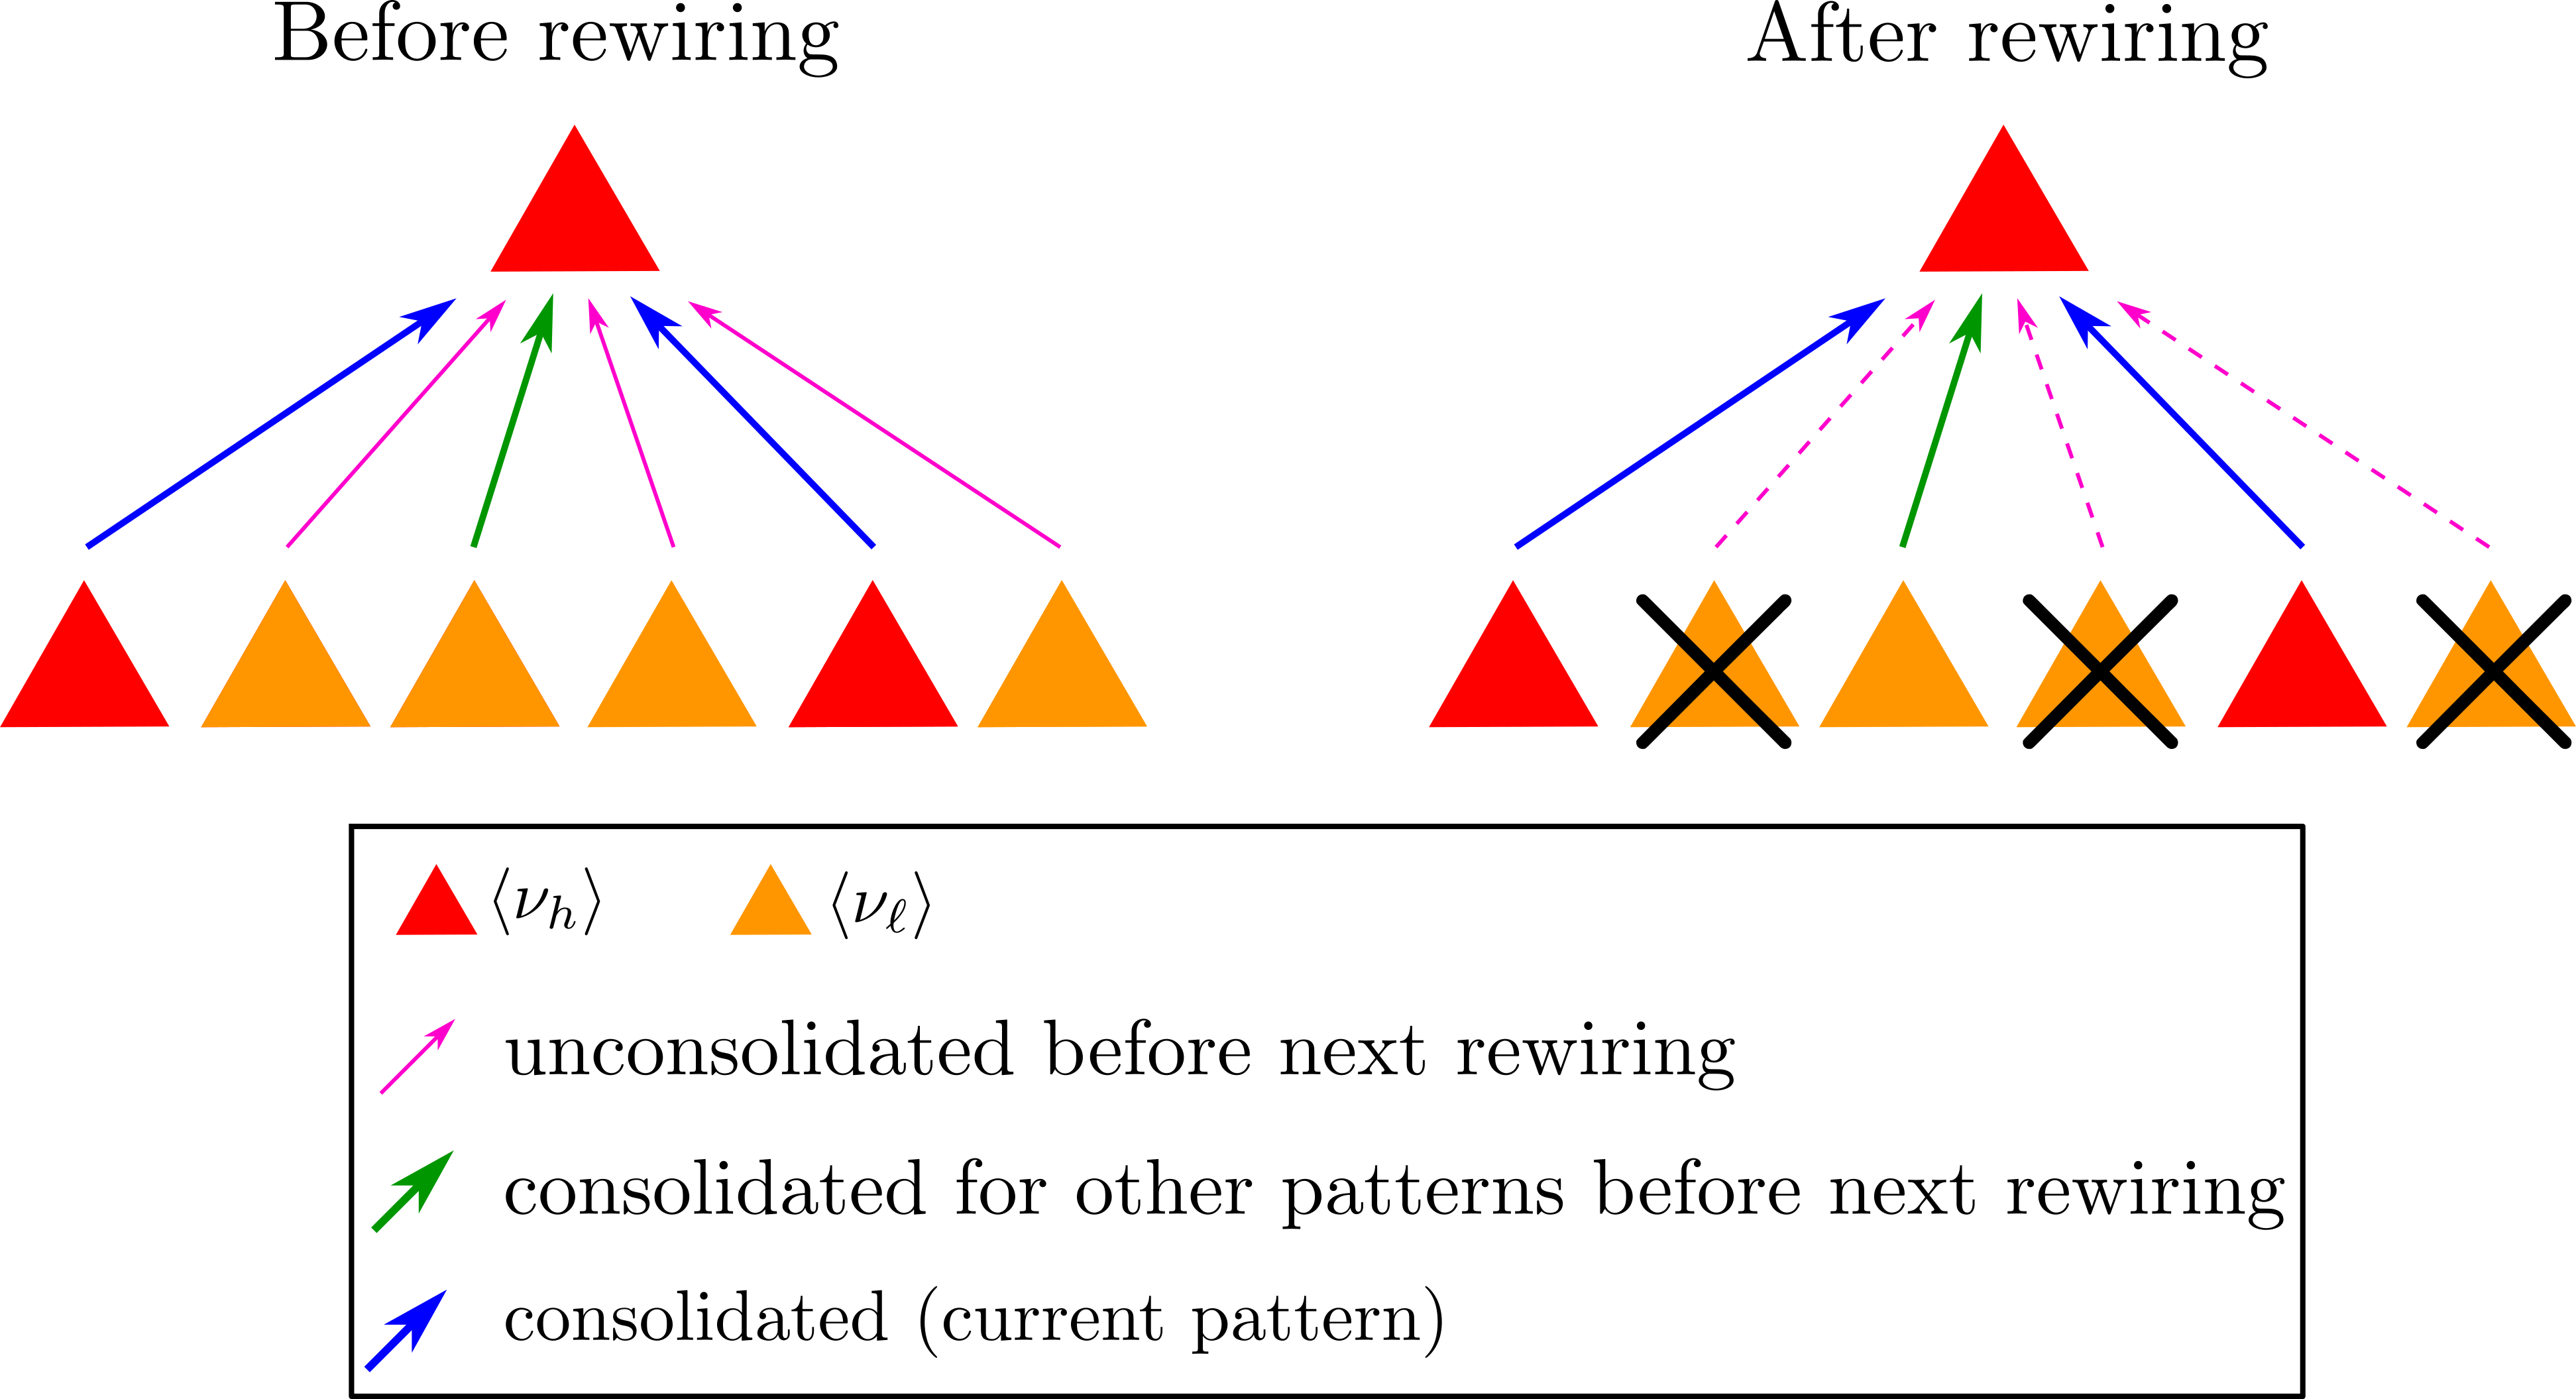
\includegraphics[width=0.8\columnwidth]{figures/rewiring.png}
\caption{
     Scheme of the rewiring process and of its effect on the average signal in input to coding neurons of the population $\popII$. Red and amber triangles represent high and low rate neurons respectively. Blue and green connections are consolidated for the current example and for a previous example, whereas pink connections are not consolidated. After rewiring these connections are pruned (here indicated with a dotted arrow), thus the relative presynaptic neurons do not project anymore to the postsynaptic neuron in exam. Figure from \cite{Tiddia2023}.
\label{fig:rewiring}}
\end{figure}

The average number of incoming connections that are consolidated in the current example (blue lines) is equal to the average number of high-rate presynaptic neurons,
$p_1 \C$.
The average number of incoming connections that are consolidated in other examples after the entire training,
$\langle k' \rangle$, is given by equation \eqref{eq:av_k1}:
\begin{equation}
    \langle k' \rangle = p \C(1-p_1)
\end{equation}
Let $t$ be the next training index for which rewiring will be applied, and $k'_t$ the number of connections from low-rate neurons that are consolidated before $t$ (green lines in the figure).
These connections will not be affected by rewiring, so even in the test phase with the same input pattern they will have low-rate presynaptic neurons.
The average value of $k'_t$ is
\begin{equation}
\label{eq:avg_k1t}
\langle k'_t \rangle = p_t \C ( 1 - p_1 )
\end{equation}
where $p_t$ is given by an expression analogous to the one obtained for $p$ (Equation \eqref{eq:p})
\begin{equation}
\label{eq:pt}
p_t = 1 - (1 - p_1 p_2)^t
\end{equation}
On the other hand, there will be $k' - k'_t$ connections displaced by rewiring and consolidated in training examples of index greater than $t$.
Putting all the contributions together, we obtain the following expression for $\SII$:

\begin{equation}
\label{eq:s2_cont_rewiring}
\begin{split}
    \langle \SII \rangle &=
    p_1 \C \Wc \langle \rh \rangle +
    ( \langle k' \rangle - \langle k'_t \rangle )
    \Wc \langle \nu \rangle
    + \langle k'_t \rangle \Wc \langle \rl \rangle
    + \Wb (\C - p_1 \C - \langle k' \rangle)
    \langle \nu \rangle =\\
    &= p_1 \C \Wc \langle \rh \rangle +
    \langle k' \rangle \Wc \langle \nu \rangle +
    \Wb [ \C (1 - p_1) - \langle k' \rangle ]
    \langle \nu \rangle
    - \langle k'_t \rangle \Wc
    ( \langle \nu \rangle - \langle \rl \rangle )
\end{split}
\end{equation}
To obtain the average value of $\SII$ over all examples, $\langle k'_t \rangle$ must be averaged over all values of the index $t$ for which rewiring is done.
This calculation is shown in Appendix \ref{app:avg_k1t}.
Equation \eqref{eq:s2_cont_rewiring} is also valid in the case for which neurons can assume discrete values of firing rate. In that case, $\langle \rl \rangle$, $\langle \rh \rangle$ and $\langle \nu \rangle$ have to be replaced with the discrete values $\rl$, $\rh$ and the average rate $\langle \nu \rangle$ shown in Table \ref{tab:discrete_model}.

\subsubsection{\label{subseq:noise} Introduction of noise into input patterns}
In a realistic learning model, the test patterns will never be exactly the same as the training ones. The ability of a learning model to generalize is linked to the ability to recognize which training pattern or patterns are most similar to a given test pattern, according to appropriate metrics.
To study the generalization capacity of the model proposed in this work, the test input patterns were generated starting from the corresponding training input patterns by adding
noise, which is represented by a deviation extracted from a given probability distribution with assigned standard deviation.
In Appendix \ref{app:noise} we describe the effect that a noise with a truncated Gaussian distribution has on the firing rates and on the variables $\Sb$, $\SII$, $\varSb$ and SDNR, and we derive the modified equations.

\subsubsection{\label{subseq:summary} Summary of theoretical model equations}
Table \ref{tab:continuous_model} summarizes the equations of the continuous rate model in case of fixed number of incoming connections per neuron. As mentioned before, when the value of $\C$ follows a Poisson distribution, $\langle\Sb\rangle$ and $\langle\SII\rangle$ are given by the same expression obtained for the fixed in-degree connection rule with $\C$ replaced by $\langle\C\rangle$. The variance of the background signal has an additional term in that case and is given by Equation \eqref{eq:var_sb_c_variable}.

\begin{table}[H]
    \centering
    \renewcommand\arraystretch{1.5}
    \begin{tabular}{
  |@{\hspace*{\marg}}m{0.3\textwidth}@{\hspace*{\marg}}
  |@{\hspace*{\marg}}m{0.1\textwidth}@{\hspace*{\marg}}
  |@{\hspace*{\marg}}m{0.6\textwidth}@{\hspace*{\marg}}
  |}
  \hline 
  \multicolumn{3}{|>{\color{white}\columncolor{black}}c|}{
  \textbf{Continuous rate model}
  }\\
  \hline 
  \textbf{Name} & \textbf{Symbol} & \textbf{Equation}\\
  \hline
  Rate distribution & $\rho(\nu)$ & $\frac{1}{\sqrt{2\pi} \sigma \nu} \cdot \exp\Bigl( -\frac{(\ln(\nu)-\mu)^2}{2\sigma^2}\Bigr)$ \\
  \hline
  Mean of the normal distribution of $\ln(\nu)$ & $\mu$ & $\ln(\langle \nu \rangle) - \frac{\sigma^2}{2}$\\
  \hline
  Standard deviation of the normal distribution of $\ln(\nu)$ & $\sigma$ & $\text{erf}^{-1}(q_1) - \text{erf}^{-1}\Big( \frac{q_1 \langle \rl \rangle}{\langle \nu \rangle} \Big)$\\
  \hline
  Rate threshold & $\rt$ & $\exp \Big(\text{erf}^{-1}(q_1)\sigma + \mu\Big)$\\
  \hline
  Average high rate & $\langle \rh \rangle$ & $\frac{1}{p_1} \int_{\rt}^{\infty} \nu \rho (\nu) d\nu$\\
  \hline
  Average low rate & $\langle \rl \rangle$ & $\frac{1}{q_1}\int_{0}^{\rt} \nu \rho (\nu) d\nu$\\
  \hline
  Average rate & $\langle \nu \rangle$ & $q_1 \langle \rl \rangle + p_1 \langle \rh \rangle $\\
    \hline
  Rate standard deviation & $\sigma_{\nu}^2$ & $\Big( e^{\sigma^2} - 1 \Big)e^{2\mu + \sigma^2}$\\
  \hline
  Average background signal & $\langle \Sb \rangle$ & $(\Wc - \Wb) \langle k \rangle \langle \nu \rangle + \Wb \C \langle \nu \rangle$\\
  \hline
  Variance of background signal & $\varSb$ & $\Bigl[ \Wc^2 \langle k \rangle + \Wb^2 (\C - \langle k \rangle)\Bigr] \sigma_{\nu}^2 + (\Wc - \Wb)^2 \sigma_{k}^2 \langle \nu \rangle ^2$\\
  \hline
  Average coding-neuron signal (without rewiring) & $\langle \SII \rangle$ & $\Wc p_1 \C \langle \rh \rangle + \Bigl[ (\Wc - \Wb) \langle k \rangle + \C \Wb \Bigr] (1-p_1) \langle \rl \rangle$ \\
  \hline
  Average coding-neuron signal (with rewiring) & $\langle \SII \rangle$ & $\Wc p_1 \C \langle \rh \rangle + \Bigl[ (\Wc - \Wb) \langle k \rangle + \C \Wb \Bigr] (1-p_1) \langle \nu \rangle - \langle k'_t \rangle \Wc
    ( \langle \nu \rangle - \langle \rl \rangle )$ \\
  \hline
  
\end{tabular}
    \caption{Summary of the equations for the continuous model. Equations shown here refers to the case in which the number of incoming connections per neuron $\C$ is constant.}
    \label{tab:continuous_model}
\end{table}


\section{Recurrent neuron model}
\label{sec:recurrent_model}
Here we describe the recurrent network model, in which population $\popII$ shows recurrent connections and projects to an inhibitory population $\popinh$ from which it receives a global inhibitory signal\footnote{N.B. this theoretical framework is still on development, additional work is required to provide an appropriate framework to be compared with computational simulations.}. Indeed, self-connections and an inhibitory feedback are fundamental ingredients to realize realistic networks oriented towards the study of learning process \cite{Coultrip1992}, and several other spiking learning models are based on a similar structure to the one depicted in Figure \ref{fig:recurrent_str_pl} (see, for example, \cite{Golosio2021-ThaCo, DeLuca2023}). Next figure depicts a scheme of the network.

\begin{figure}[h]
    \centering
    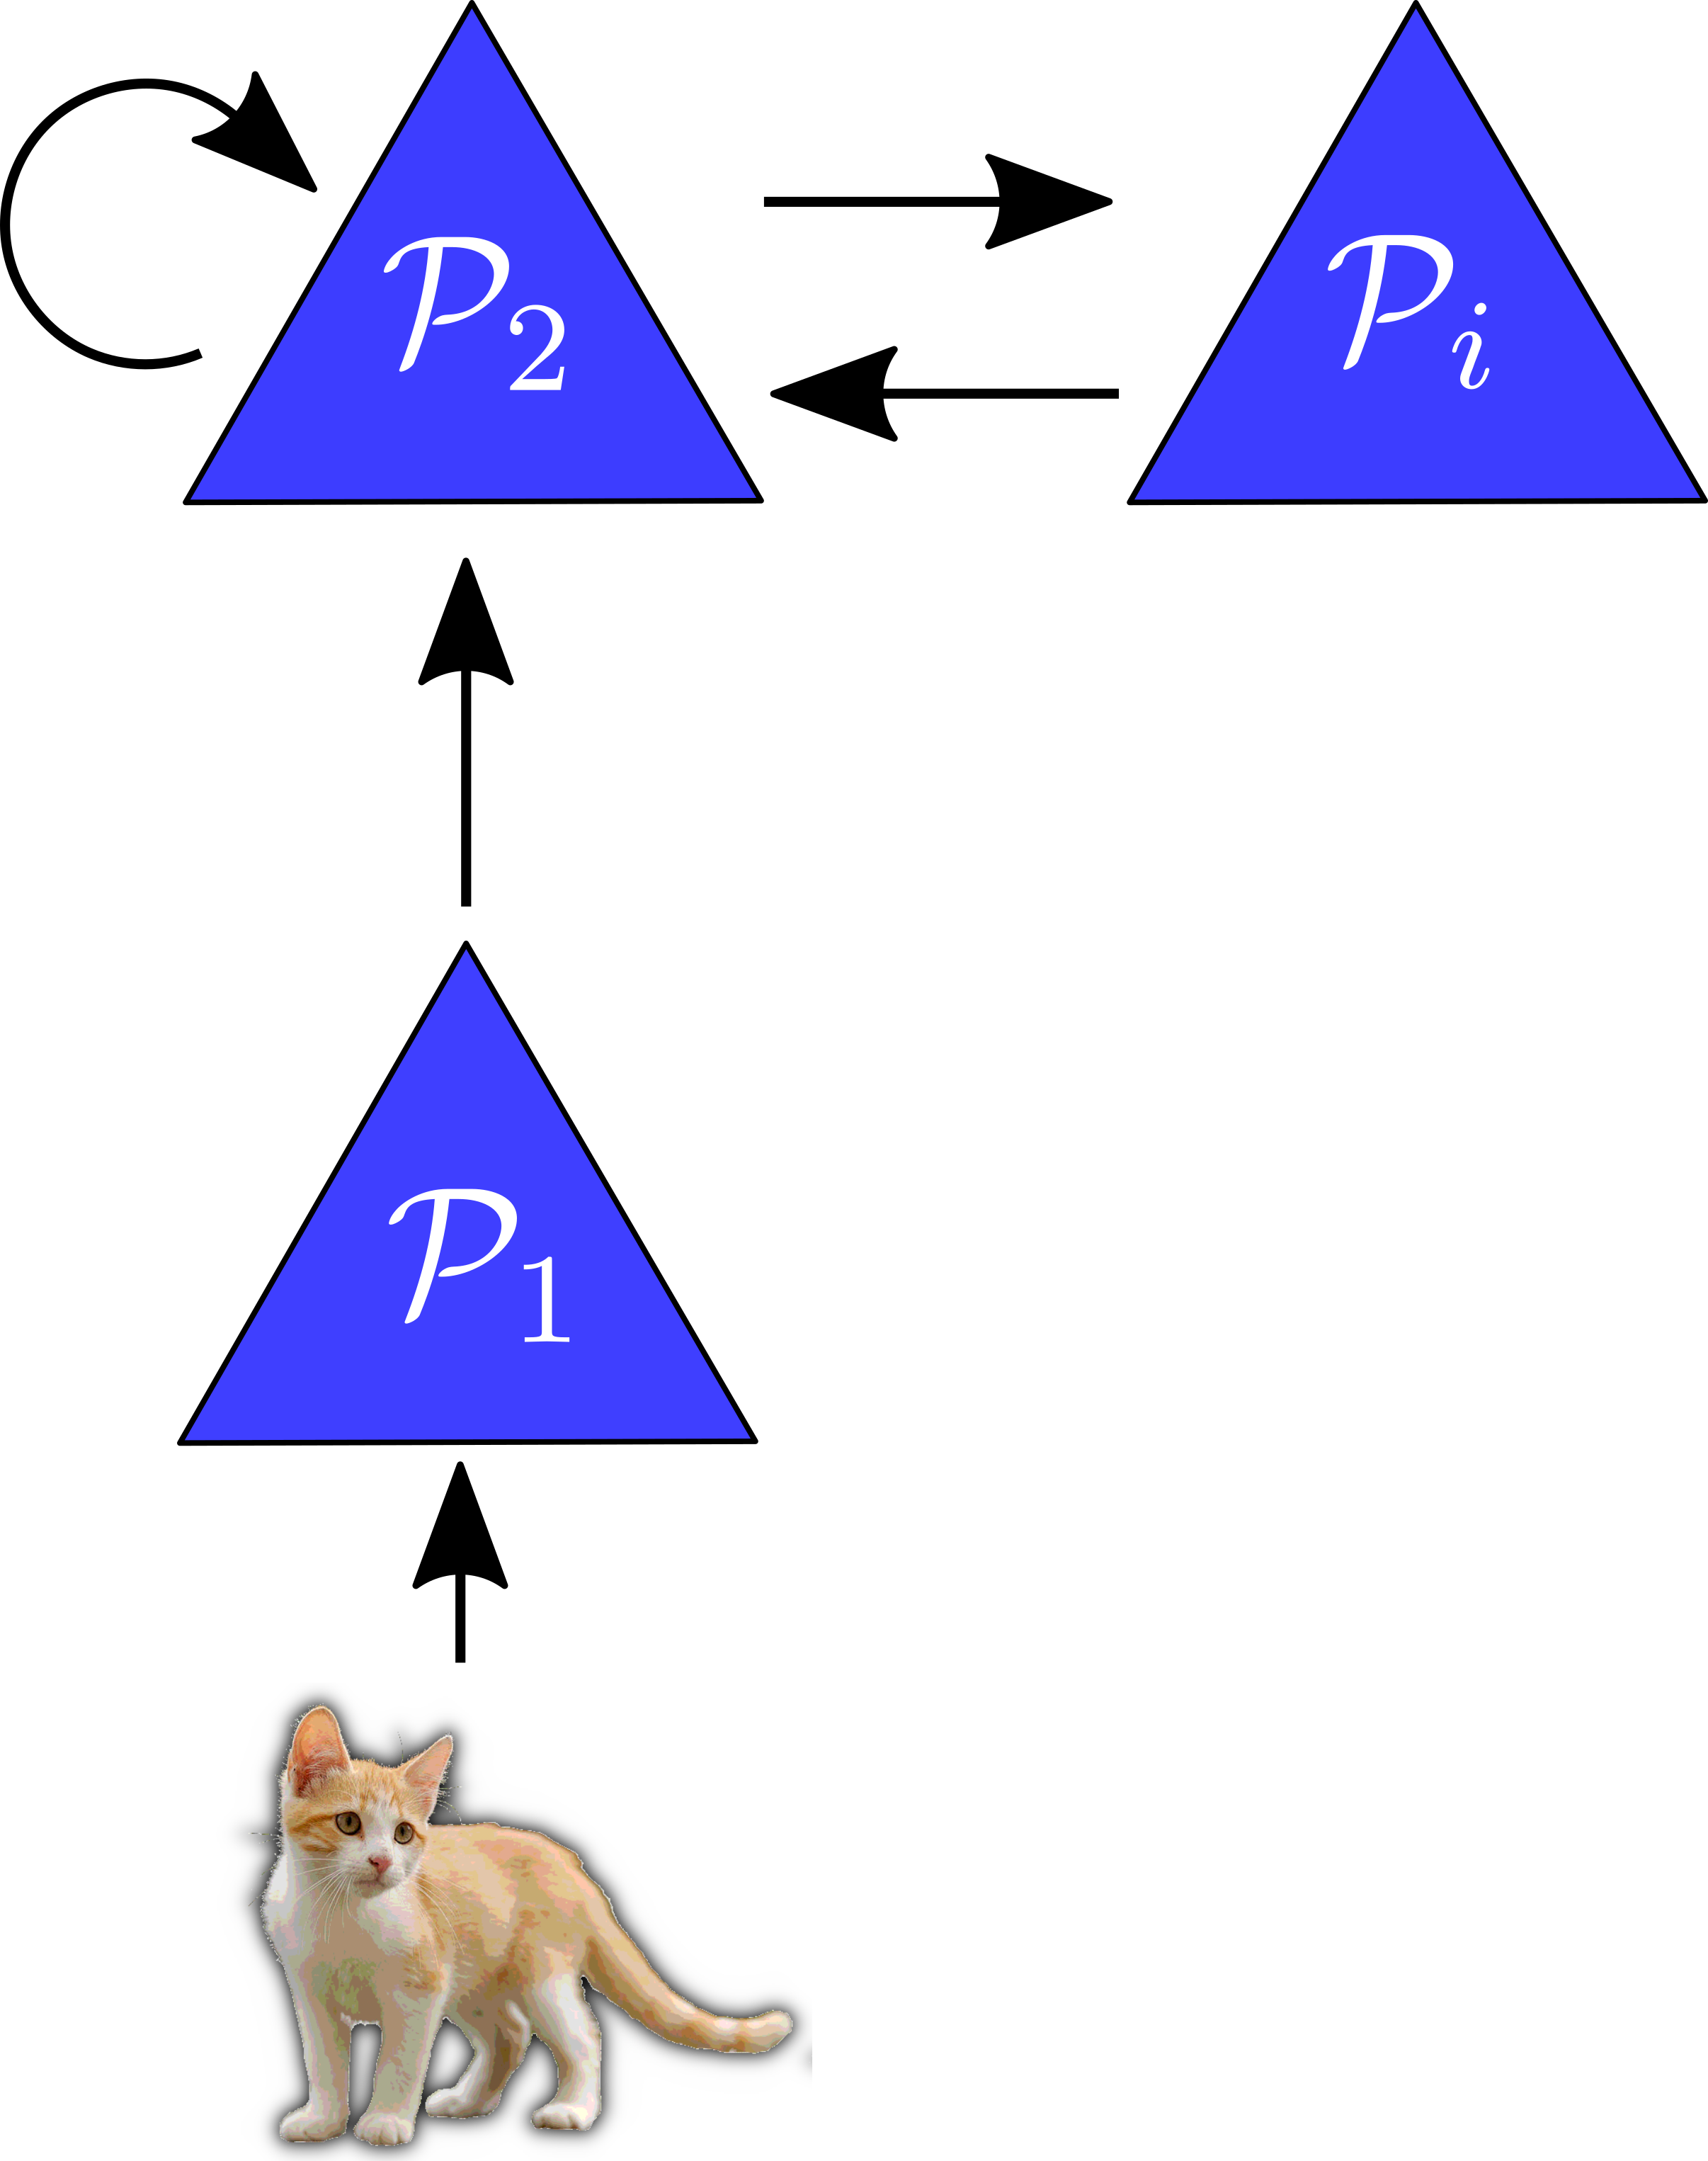
\includegraphics[width=0.4\columnwidth]{figures/recurrent.png}
    \caption{Schematic representation of the recurrent network model through a block diagram.}
    \label{fig:recurrent_str_pl}
\end{figure}

In this case, we follow an approach similar to the one proposed in Section \ref{sec:firing_rate_models}, in particular describing each population with a differential equation of the average rate similar to Equations \eqref{eq:feed_forward} and \eqref{eq:recurrent}, in which every population is provided with time constant $\tau$ needed to describe the time needed for the population to reach a steady state firing rate. In this case, only the time constant between excitatory and inhibitory population is distinguished. 


In this section we derive the expressions for the background signal $\Sb$ and coding neuron signal $\SII$ to the neurons of population $\popII$. To this aim, several input average rates $y_i$ have to be considered:

\begin{itemize}
    \item $y_0$: average input rate from non-coding neurons and non consolidated connections;
    \item $y_1$: average input rate from non-coding neurons and consolidated connections;
    \item $y_2$: average input rate from coding neurons and non consolidated connections;
    \item $y_3$: average input rate from coding neurons and consolidated connections;
    \item $y_4$: average input rate from inibitory neurons.
\end{itemize}

The reason for such an input grouping will be clear with the following derivation of the equations for $\Sb$ and $\SII$. The differential equations describing the listed average rates is, accordingly to Section \ref{sec:firing_rate_models}

\begin{equation}
\label{eq:eq_diff_campo_medio}
    \tau_i \dfrac{d y_i}{dt}= -y_i + \mathcal{F}\Bigl( \sum_{j=0}^{4} W_{ij} y_j+E_i-S_{\text{th},i}\Bigr)
\end{equation}

Where $\tau_i$ is the time constant for the input $i$, $W_{ij}$ is the matrix of the synaptic weights multiplied by the average number of indegrees from the population $j$ to population $i$, $E_i$ is the input rate from other populations, including the input coming from $\popI$, and $S_{\text{th},i}$ represent the activation threshold for the neuron population $i$ and, eventually, $\mathcal{F}$ is the activation function. Choosing the ReLU (see Equation \eqref{eq:ReLu}) as activation function, a reasonable assumption we can do is considering to be over threshold for every neuron population, since both excitatory and inhibitory neurons show a significant activity also during rest. Thus, the ReLu can be reduced to a linear function
\begin{equation}
     \mathcal{F}(x)= \alpha x H(x) = \alpha x  \qquad \text{with} \quad x=\sum_{j=0}^{4} W_{ij} y_j+E_i-S_{\text{th},i} \quad \text{and} \quad x>0
\end{equation}

Hence, Equation \eqref{eq:eq_diff_campo_medio} becomes

\begin{equation}
    \tau_i \frac{d y_i}{dt}= -y_i + \alpha \Bigl( \sum_{j=0}^{4} W_{ij} y_j+E_i-S_{\text{th},i}\Bigr)
\end{equation}

Now we can rewrite the equation in a matrix form. Given $C_{ij}= \frac{1}{\tau_i} ( - \delta_{ij} + \alpha W_{ij})$ and $b_i= \frac{\alpha}{\tau_i} (E_i - S_{\text{th},i})$ we have

\begin{equation}
   \dfrac{d y_i}{dt}=  \sum_{j=0}^{4} C_{ij} y_j+b_i
\end{equation}

which can be written as follows
\begin{equation}
    \frac{d \vec{y}}{dt} = C \vec{y}+ \vec{b}
\end{equation}

Here we focus on the study of the steady state of the previous equation, in which the average firing rates of the different neuron populations do not change anymore over time. Thus, we can set the derivative of Equation \eqref{eq:eq_diff_campo_medio} to zero, obtaining

\begin{equation}
\label{eq:asintotic_condition}
    0= - y_i + \alpha( \sum_{j=0}^{4} W_{ij} y_j+E_i-S_{\text{th},i})
\end{equation}

from which we can obtain a matrix equation in which we have to solve for the average rates $y_i$:

\begin{equation}
\begin{gathered}
y_i-\alpha \sum_{j=0}^{4} W_{ij} y_j = \alpha (E_i- S_{\text{th},i})\\
                                    (I-A) \vec{y}=\vec{b} \qquad  \Longrightarrow \qquad \vec{y}= M^{-1} \vec{b}  \\ 
\text{with} \qquad A_{ij}=\alpha  W_{ij}    \quad \text{and} \quad b_{i}=\alpha (E_i-S_{\text{th},i}) \quad \text{and} \quad M=I-A
\end{gathered}
\end{equation}

Thus, we can solve this equation by computing $M^{-1}$. Before obtaining the equations for $\langle\Sb\rangle$ and $\langle\SII\rangle$ we should motivate the introduction of the four different rates $y_i$ instead of having neurons with only high or low rates $\rh$ and $\rl$. The distinction between these four input rates is necessary because of self connections. Indeed, there is a correlation between connection consolidation and average input rate. We present an example to make this clear. 


Let us considering some neurons of population $\popII$ when the network is trained with $\T=10^5$ patterns. Having a probability $p_2= 10^{-3}$ for a neuron to be representative for a pattern, this means that, on average, a neuron will be representative for $\langle m \rangle = 10$ patterns. The variable $m$ will have a variance $\sigma^2_{m}\propto \sqrt{m}$, hence some neurons can be representative for more than 10 patterns, and consequently these neurons will have more consolidated connections both in input and output due to the self-connections. Thus, neurons with higher $m$ have more consolidated connections, ergo they are likely to show a higher firing rate. This way a correlation between average rate and number of synaptic connections takes place, and the theoretical framework should take account of such a correlation. In order to show that, we need to do some calculations similar to the ones reported in Appendix \ref{app:var_k} in which we compute the variance of the number of consolidated connections $k$ for the feed-forward model. In particular, we need to remember that $Q(m,h)$ (see Equation \eqref{eq:Q_mk}) represents the probability that a neuron of $\popII$ is representative for $m$ patterns and has $h$ consolidated indegrees from neurons of $\popI$. Analogously, we can derive an expression to represent the probability for a neuron of $\popI$ to be representative for $m$ patterns and with $h$ consolidated outdegree to neurons of $\popII$. 
In the following we call $C_{12}^\text{in}$ the average number of connections in input for a neuron of $\popII$ coming from population $\popI$, and $C_{12}^\text{out}$ the number of outcoming connections to neurons of $\popII$ from each neuron of $\popI$. Generally speaking, $C_{12}^\text{in} \neq C_{12}^\text{out}$ since the number of neurons of the two populations might differ. However, the outcoming connections from $\popI$ to $\popII$ should equate the incoming connections to $\popII$ from $\popI$, hence

\begin{equation}
\NII C_{12}^\text{in} = \NI C_{12}^\text{out}
\end{equation}

Similarly, we can define $C_{22}^\text{in}$ and $C_{22}^\text{out}$, but since input and output population is the same we should have

\begin{equation}
C_{22}^\text{in} = C_{22}^\text{out} = C_{22} 
\end{equation}

Now let us define $Q_{12}^\text{out}(m,h)$ the probability that a neuron of $\popI$ is selective for $m$ patterns over $\T$ and with $h$ outcoming consolidated connections over $C_{12}^\text{out}$ to $\popII$, and $Q_{12}^\text{in}(m,h)$ the probability for a neuron of $\popII$ to be selective for $m$ patterns over $\T$ and with $h$ incoming consolidated connections over $C_{12}^\text{in}$ from $\popI$. Self-connections of $\popII$ will be discussed considering that input and output populations are the same.

The number of outcoming connections from neurons of $\popI$ representative for $m$ patterns over $\T$ is

\begin{equation}
     H_{12}^\text{out}(m) = \NI \sum_{h} h Q_{12}^\text{out}(m,h)
     = N_1 \xi_{12}^\text{out} (m) 
\end{equation}

where

\begin{equation}
\xi_{12}^\text{out} (m) = 
 \sum_{h} \hspace{1mm}  h \hspace{1mm} Q_{12}^\text{out}(m,h)
\end{equation}

The total number of consolidated connections is thus

\begin{equation}
     H_{12}^\text{tot} = \sum_{m} H_{12}^\text{out}(m) = N_1 \sum_{m,h} h  Q_{12}^\text{out}(m,h) = \NI \langle h_{12}^\text{out} \rangle
\end{equation}

This way, we can compute the probability $p_{12}^\text{out}(m)$ that a consolidated connection has a presynaptic neuron which is representative for $m$ patterns

\begin{equation}
    p_{12}^\text{out}(m) = \frac{H_{12}^\text{out}(m)}{H_{12}^\text{tot}} =
    \frac{\NI \xi_{12}^\text{out} (m)}{N_1 \langle h_{12}^\text{out} \rangle}= \frac{\xi_{12}^\text{out} (m)}{\langle h_{12}^\text{out} \rangle}
\end{equation}

Similarly, the number of non consolidated connections outgoing from neurons of $\popI$ representative for $m$ patterns is

\begin{equation}
     Z_{12}^\text{out}(m) 
     = \NI \sum_{h}  
     (C_{12}^\text{out} - h) Q_{12}^\text{out}(m,h) 
     = \NI \zeta_{12}^\text{out} (m) 
\end{equation}

where

\begin{equation}
     \zeta_{12}^\text{out} (m) =
     \sum_{h}  
     (C_{12}^\text{out} - h)Q_{12}^\text{out}(m,h) 
\end{equation}

The total number of connections is 

\begin{equation}
     Z_{12}^\text{tot} = \sum_{m} Z_{12}^\text{out}(m) = \NI \sum_{m,h} (C_{12}^\text{out} - h) Q_{12}^\text{out}(m,h) = \NI (C_{12}^\text{out} - \langle h_{12}^\text{out} \rangle)
\end{equation}

and thus the probability $q_{12}^\text{out}(m)$ that a non consolidated connection is outgoing from a neuron representative for $m$ patterns is

\begin{equation}
    q_{12}^\text{out}(m) = \frac{Z_{12}^\text{out}(m)}{Z_{12}^\text{tot}} =
    \frac{\NI \zeta_{12}^\text{out} (m)}{N_1 (C_{12}^\text{out}-\langle h_{12}^\text{out} \rangle)}= \frac{\zeta_{12}^\text{out} (m)}{C_{12}^\text{out}-\langle h_{12}^\text{out} \rangle}
\end{equation}

The probability that a neuron of $\popI$ is selective for $m$ patterns is

\begin{equation}
    G_1(m) = \sum_{h=0}^{C_{12}^\text{out}} Q_{12}^\text{out}(m,h)
\end{equation}

and multiplying the latter to $\NI$ we get the total number of neurons of $\popI$ representative for $m$ patterns. Remembering that $\NI \xi_{12}^\text{out}(m)$ represents the total number of consolidated connections from neurons of $\popI$ representative for $m$ patterns, the average number of consolidated connections outcoming from a neuron of $\popI$ representative for $m$ patterns is

\begin{equation}
\label{eq:kout_m_T}
    \kappa_{12}^\text{out} (m)= \frac{\NI \xi_{12}^\text{out}(m)}{\NI G_1(m)}
    = \frac{\xi_{12}^\text{out}(m)}{G_1(m)}
\end{equation}

The equation above can be reduced to the following

\begin{equation}
    \kappa_{12}^\text{out} (m)=C_{12}^\text{out} \Bigl[ 1- (1-p_2)^m\Bigr]
\end{equation}

where $p_2$ represents the probability for a neuron of $\popII$ of being selective for a pattern.


Using a similar procedure, it is possible to obtain the average number of consolidated connections incoming to a neuron of $\popII$ representative for $m$ patterns from neurons of $\popI$:

\begin{equation}
\label{eq:kin_m}
    \kappa_{12}^\text{in} (m)=C_{12}^\text{in} \Bigl[ 1- (1-p_1)^m\Bigr]
\end{equation}

and the average number of consolidated connections to neurons of $\popII$ coding for $m$ patterns and coming from neurons of the same population is

\begin{equation}
\label{eq:k22_m}
    \kappa_{22} (m)=C_{22} \Bigl[ 1- (1-p_2)^m\Bigr]
\end{equation}

Notice that in this case the average number of incoming or outcoming consolidated connections is the same.

Previous expressions show that the average number of consolidated connections, both incoming and outcoming, is higher for neurons representative for more patterns (i.e., higher $m$), as anticipated.


Now that we have an expression for the average number of consolidated connections coming from different neuron populations, we can derive the values of $\Sb$ and $\SII$. We use the following notation to refer to the average input rates for the self connections of $\popII$:

\begin{itemize}
    \item $r_{l,2}^{\text{nc}}$: average input rate to non consolidated connections outgoing from non representative neurons for the current pattern;
    \item $r_{l,2}^{\text{c}}$: average input rate to consolidated connections outgoing from non representative neurons for the current pattern;
    \item $r_{h,2}^{\text{nc}}$: average input rate to non consolidated connections outgoing from representative neurons for the current pattern;
    \item $r_{h,2}^{\text{c}}$: average input rate to consolidated connections outgoing from representative neurons for the current pattern;
    \item $r_\text{I}$: average input rate of inhibitory neurons.
\end{itemize}

The average input to a non representative neuron of $\popII$ having $\kappa_{22}$ consolidated indegrees from the same population and $\kappa_{12}$ consolidated indegrees from neurons of $\popI$ can be computed as discussed in the feed-forward model. The only difference here is the addition of the different average rates for consolidated or non consolidated connections. Thus, we can compute the background signal $\Sb$ in input to a neuron of $\popII$ as follows:

\begin{equation}
\label{eq:sb_selfconnected}
\begin{split}
    \mathcal{S}_{b,2} (\kappa_{12}, \kappa_{22}) &=
    \Wc \kappa_{22} r_{\text{av},2}^{\text{c}}+ \Wb (C_{22}-\kappa_{22}) r_{\text{av},2}^{\text{nc}} +\\ &+
    \Wc \kappa_{12} r_{\text{av},1} 
    + \Wb (C_{12}^\text{in}-\kappa_{12}) r_{\text{av},1} +
    \WIE C_\text{IE} r_\text{I} + E \\
\end{split}
\end{equation}

where $r_{\text{av},1}$ is the average rate of the neurons of $\popI$, and $r_{\text{av},2}^{\text{c}}$ is the average rate from other neurons of $\popII$ that are representative for the current pattern and connected with consolidated connections. Similarly, $r_{\text{av},2}^{\text{nc}}$ is the average rate from neurons of $\popII$ connected with non consolidated connections. $\WIE$ is the synaptic weight for the inhibitory-to-excitatory connections, and 
$C_\text{IE}$ is the average number of connections to a neuron of $\popII$ coming from the inhibitory population $\popinh$. Finally, $E$ is the average input signal from other populations. The first two terms of Equation \eqref{eq:sb_selfconnected} represent the contribution due to the self connections, whereas the third and the fourth are the contributions of $\popI$ to the input, ergo the same expression that represented $\Sb$ in the feed-forward model. Eventually, the last two terms are related to external stimulation and inhibitory feedback.


The two average rates $r_{\text{av},2}^{\text{c}}$ and $r_{\text{av},2}^{\text{nc}}$ can be written in term of the rate previously listed (i.e., $r_{h,2}^{\text{c}}$, $r_{l,2}^{\text{c}}$ ,$r_{h,2}^{\text{nc}}$ and $r_{l,2}^{\text{nc}}$) following the expression:

\begin{equation}
    \begin{cases}
     r_{\text{av},2}^{\text{c}}= p_2 r_{h,2}^{\text{c}}+ (1-p_2)r_{l,2}^{\text{c}}\\
     r_{\text{av},2}^{\text{nc}}= p_2 r_{h,2}^{\text{nc}}+ (1-p_2)r_{l,2}^{\text{nc}}
    \end{cases}
\end{equation}

The average rates have a linear dependence from $\kappa_{12}$ and $\kappa_{22}$ because of the fact that in Equation \eqref{eq:asintotic_condition} we have a term like $\mathcal{S}_{b,2}(\kappa_{12},\kappa_{22}) - S_{\text{th},i}$. The linearity enables us to write the different rates as

\begin{equation}
\begin{cases}
    r_{l,2}^{\text{c}}  =   
        r_{l,2} (\langle \kappa_{12} {\rangle}_\text{cons},
        \langle \kappa_{22} {\rangle}_\text{cons}) \\
    r_{h,2}^{\text{c}}  =
        r_{h,2} (\langle \kappa_{12} {\rangle}_\text{cons},
        \langle \kappa_{22} {\rangle}_\text{cons})  \\
    r_{l,2}^{\text{nc}}  =
        r_{l,2} (\langle \kappa_{12} {\rangle}_\text{nocons},
        \langle \kappa_{22} {\rangle}_\text{nocons}) \\
    r_{h,2}^{\text{nc}}  =
        r_{h,2} (\langle \kappa_{12} {\rangle}_\text{nocons},
        \langle \kappa_{22} {\rangle}_\text{nocons})  \\
\end{cases}
\end{equation}

where expectation values refers to presynaptic neurons of consolidated or non consolidated self connections of $\popII$.


To compute $\langle \kappa_{12}{\rangle}_\text{cons}$ we can refer to Equation \eqref{eq:kin_m} for 
$\kappa_{12}^\text{in}(m)$,
representing the average number of consolidated connections from neurons of $\popI$ to a neuron of $\popII$ representative for $m$ patterns. Starting from that equation, we have to do a weighted average over $m$ taking account of the probability that a consolidated self connection of $\popII$ comes from a representative neurons for $m$ patterns, to that

\begin{equation}
    \langle \kappa_{12} \rangle_{\text{cons}} = \sum_{m=0}^{\T} p_{22}(m)
    \kappa_{12}^\text{in}(m)
    = \sum_{m=0}^{\T} \frac{\xi_{22}(m)}{\langle h_{22} \rangle}
    \kappa_{12}^\text{in}(m)
\end{equation}

Analogously, we can derive the expectation value of $\kappa_{12}$ for presynaptic neurons of non consolidated self connections

\begin{equation}
    \langle \kappa_{12} \rangle_{\text{nocons}} =  \sum_{m=0}^{\T} q_{22}(m)
    \kappa_{12}^\text{in}(m)
    = \sum_{m=0}^{\T} \frac{\zeta_{22}(m)}{C_{22} -\langle h_{22} \rangle}
    \kappa_{12}^\text{in}(m)
\end{equation}

The expressions for
$\langle \kappa_{22} \rangle_{\text{cons}}$ and $\langle \kappa_{22} \rangle_{\text{nocons}}$ can be obtained in a similar way:

\begin{equation}
    \langle \kappa_{22} \rangle_{\text{cons}} = 
    \sum_{m=0}^{\T} \frac{\xi_{22}(m)}{\langle h_{22} \rangle}
    \kappa_{22}(m)
\end{equation}

\begin{equation}
    \langle \kappa_{22} \rangle_{\text{nocons}} =   \sum_{m=0}^{\T} \frac{\zeta_{22}(m)}{C_{22} -\langle h_{22} \rangle}
    \kappa_{22}(m)
\end{equation}

After a few calculations (not reported here) it is possible to obtain the expressions for
$\langle \kappa_{12} \rangle_{\text{cons}}$,
$\langle \kappa_{12} \rangle_{\text{nocons}}$,
$\langle \kappa_{22} \rangle_{\text{cons}}$ e
$\langle \kappa_{22} \rangle_{\text{nocons}}$
as a function of the probability of being representative for a pattern as a neuron of $\popI$ or $\popII$, i.e., $p_1$ and $p_2$:

\begin{equation}
\begin{gathered}
    \langle \kappa_{12} \rangle_{\text{cons}}= C_{12}^\text{in} \frac{
    1 - (1-p_{1} p_{2})^\T
    -(1-p_{2}^2)^\T
    +(1 - p_{1} p_{2} - p_{2}^2
    + p_{1} p_{2}^{2})^\T}
    {1-(1-p_{2}^2)^\T} \\
    \langle \kappa_{12} \rangle_{\text{nocons}}= C_{12}^\text{in} \Bigl[1-\Bigl(\frac
    {1- p_{1} p_{2} - p_{2}^2 + p_{1} p_{2}^{2}}{1-p_{2}^2} \Bigr)^\T \Bigr] \\
    \langle \kappa_{22} \rangle_{\text{cons}}= C_{22} \frac{1-2(1-p_{2}^2)^\T+(1-2p_{2}^2+p_{2}^{3})^\T}{1-(1-p_{2}^2)^\T} \\
    \langle \kappa_{22} \rangle_{\text{nocons}}= C_{22} \Bigl[1-\Bigl(\frac{1-2p_{2}^2+p_{2}^{3}}{1-p_{2}^2} \Bigr)^\T \Bigr]
\end{gathered}
\end{equation}

These expressions should replace the term $\kappa_{12}$ and $\kappa_{22}$ in Equation \eqref{eq:sb_selfconnected} for $\mathcal{S}_{b,2}$ to find the average input signal for non representative neurons of $\popII$. The calculation for the average input signal to representative neurons of $\popII$, i.e., $\mathcal{S}_{2,2}$ can be obtained using similar techniques and properly replacing the rate contributions due to the self connections of $\popII$.





\chapter{\textbf{Learning through structural plasticity: firing rate-based network simulations}}
\label{chapter:structural_plasticity_simulation}

\begin{tcolorbox}[colback=white,colframe=DarkRed,title=\textbf{Summary}]
This chapter presents the simulations of the network of firing-rate-based neurons designed following the theoretical framework described in the previous chapter with the aim of validating the theoretical estimations. The simulation framework has been formalized by Bruno Golosio, me and Luca Sergi, a Master student. Luca Sergi and me performed the simulations and cured the data analysis.
\end{tcolorbox}

The validation of the equations derived in the previous chapter is done through simulations with firing-rate-based neuronal network models.
The code of the simulator was written in the C++ programming language and was compiled with GCC (\url{https://github.com/gcc-mirror/gcc}) (version 10.2.0) and with GSL (\url{https://www.gnu.org/software/gsl/}) (version 2.7) scientific libraries.
The simulations have been performed using the supercomputers Galileo 100 and JUSUF \cite{JUSUF}.
The networks used for the simulations are generated according to the selected connection rule. In particular, in the case of the fixed-indegree rule, $\C$ incoming connections are created for each neuron of the $\popII$ population, where $\C$ has a fixed value.
In the case of the Poisson-indegree rule, for each neuron of the population $\popII$ the number of incoming connections $C$ is extracted from a Poisson distribution with mean $\langle C \rangle$.
In both cases, the indexes of the presynaptic neurons are randomly extracted on the $\popI$ population. 
The connection weights are initially set to the baseline value, $\Wb$.
Each training input patterns of the discrete model is generated by extracting, for each neuron of $\popI$, a random number $r$ from a uniform distribution in the interval $[0, 1]$; if $r<p_1$ the rate of the neuron is set to the high level, $\rh$, otherwise it is set to $\rl$.
An analogous procedure is used to generate the corresponding contextual stimulus pattern on the neurons of the population $\popII$.
A connection is consolidated in a training example if both the presynaptic and the postsynaptic neuron are in the high-rate level, $\rh$.
In the continuous case, the firing rates of the input pattern and those of the contextual pattern are extracted from a log-normal distribution. In this case, a connection is consolidated if the firing rates of both the presynaptic and postsynaptic neurons are above the thresholds $\nu_{t,1}$ and $\nu_{t,2}$, respectively.
Connection rewiring is performed every $s$ training steps, as described in Section \ref{subseq:rewiring}.
The test set is generated by randomly extracting $V$ input patterns from the train set. In the discrete case, the patterns are not modified. In the continuous case, the patterns of the test set are altered by adding noise extracted from a truncated Gaussian distribution.


To estimate $\langle\Sb\rangle$ and $\langle\SII\rangle$ we compute the input of each $\popII$ neuron as the sum of the rate of the presynaptic neurons of its incoming connections multiplied by the synaptic weights (i.e., $\Wc$ or $\Wb$). 
The variance $\varSb$ is evaluated by the formula

\begin{equation}
    \varSb = \langle\Sb^2\rangle - \langle\Sb\rangle^2
\end{equation}

where the mean values are calculated over the input signals to all non-coding neurons of $\popII$.

\section{Two neuron population simulations}
This section, presented also in \cite{Tiddia2023}, compares the results of the simulations of the firing rate model with the theoretical predictions described in the previous chapter. Since we proposed several versions of the model, with different features implemented, the section is divided into different parts that sum up the main characteristics of the model.
We present the results of the approaches employing discrete and continuous values for neuron firing rates, comparing the theoretical values of the average input signal to background neurons $\langle\Sb\rangle$, the average input signal to coding neurons $\langle\SII\rangle$, the variance of the background input signal $\varSb$ and the signal-difference-to-noise ratio with the values obtained from the simulations.
This way, we are able to assess the capacity of the population $\popII$, and thus of the network, to recognize a pattern memorized in the training phase.
Here, we present simulation results with a Poisson-driven number of incoming connections, with $\langle\C\rangle=5000$. We opted for such an approach since it is more realistic for biological neural circuits with respect to a fixed amount of connections per neuron. Each simulation is repeated $10$ times using a different seed for random number generation to ensure the robustness of the simulation results. The values shown in the plots are a result of averaging over the different seeds.

\subsection{Comparison between continuous and discrete firing rate}
As previously mentioned, the main difference in calculating
$\langle\Sb\rangle$ and $\langle\SII\rangle$ with the continuous rate model versus the discrete model is that the discrete values of $\nu_l$ and $\nu_h$ are replaced, respectively, by the average values of the rate below and above threshold, calculated on the continuous probability distribution.
On the other hand, the variance of the background signal differs in the two models, because it depends on the variance of the rate, $\sigma^2_{\nu}$, which is different in the two cases.\\
The first study we present is oriented towards the estimation of these parameters as a function of the number of training patterns $\T$.
As the number of training patterns increases, so does the number of patterns encoded by each individual neuron.
Since $p_2$ is the probability that a neuron of $\popII$ is in a high-rate level for a single training pattern, on average such neuron will encode $p_2 \T$ patterns of the entire training set.
This multiple selectivity of individual neurons is also present in biological neural networks, in which the same neuron can be selective for several stimuli \cite{Rigotti2013}.\\
The test set consists of $V = 1000$ input patterns, generated as described in the Materials and Methods section.
Thus, the simulation outcome used for our analysis is an average over the entire test set of the $\Sb$, $\SII$, $\varSb$ and SDNR values obtained for each test pattern.
Figure \ref{fig:discr_vs_contin} shows the comparison of the simulation outcomes using discrete and continuous rate values.

\begin{figure}[H]
\centering
	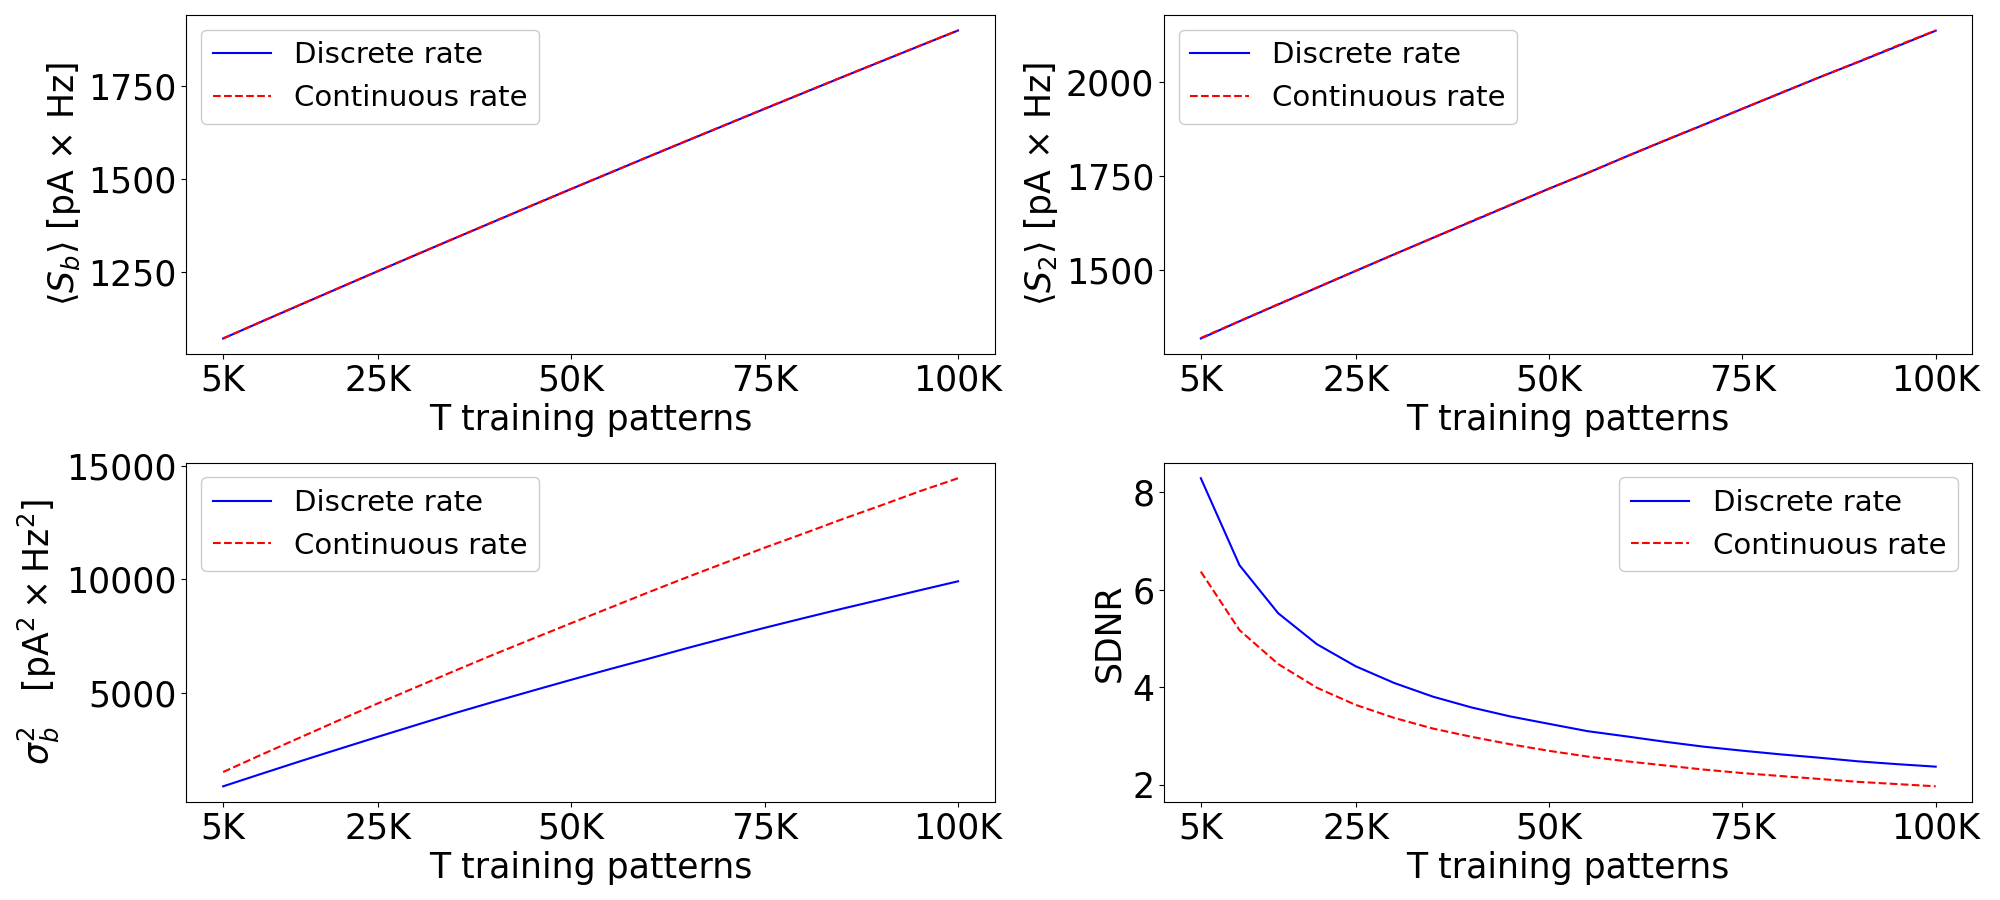
\includegraphics[width=\columnwidth]{figures/discrete_vs_continuous.png}
	\caption{ 
	Comparison between $\langle\Sb\rangle$, $\langle\SII\rangle$, $\varSb$ and SDNR obtained from simulations using discrete (blue line) or continuous (red dotted line) firing rate distribution. The values are given as a function of the number of training patterns $\T$.
	\label{fig:discr_vs_contin}}
\end{figure}

We can see that the curves of $\langle\Sb\rangle$ and $\langle\SII\rangle$ obtained from the simulations using the continuous firing rate distribution are superimposed
on those obtained using the discrete model; this is due to the fact that the choice of the threshold on the log-normal distribution is done so that the average values for low and high rate, $\langle \nu_l \rangle$ and 
$\langle \nu_h \rangle$, correspond to the values adopted in the discrete rate model.
On the other hand, the variance of the background signal $\varSb$ differs in the two models, because it depends on the variance of the firing rate,
$\sigma_\nu$, which is different in the two cases.
This leads also to the different behavior of the SDNR.

\subsection{Comparison between theoretical predictions
and simulation results}
The results shown in the previous section are obtained from simulations. This section presents a comparison between simulation results and theoretical expectations.
To provide a quantitative estimation of the discrepancy between the theoretical predictions and the simulations, we evaluate their relative error, using the theoretical values as a reference.

\begin{figure}[H]
\centering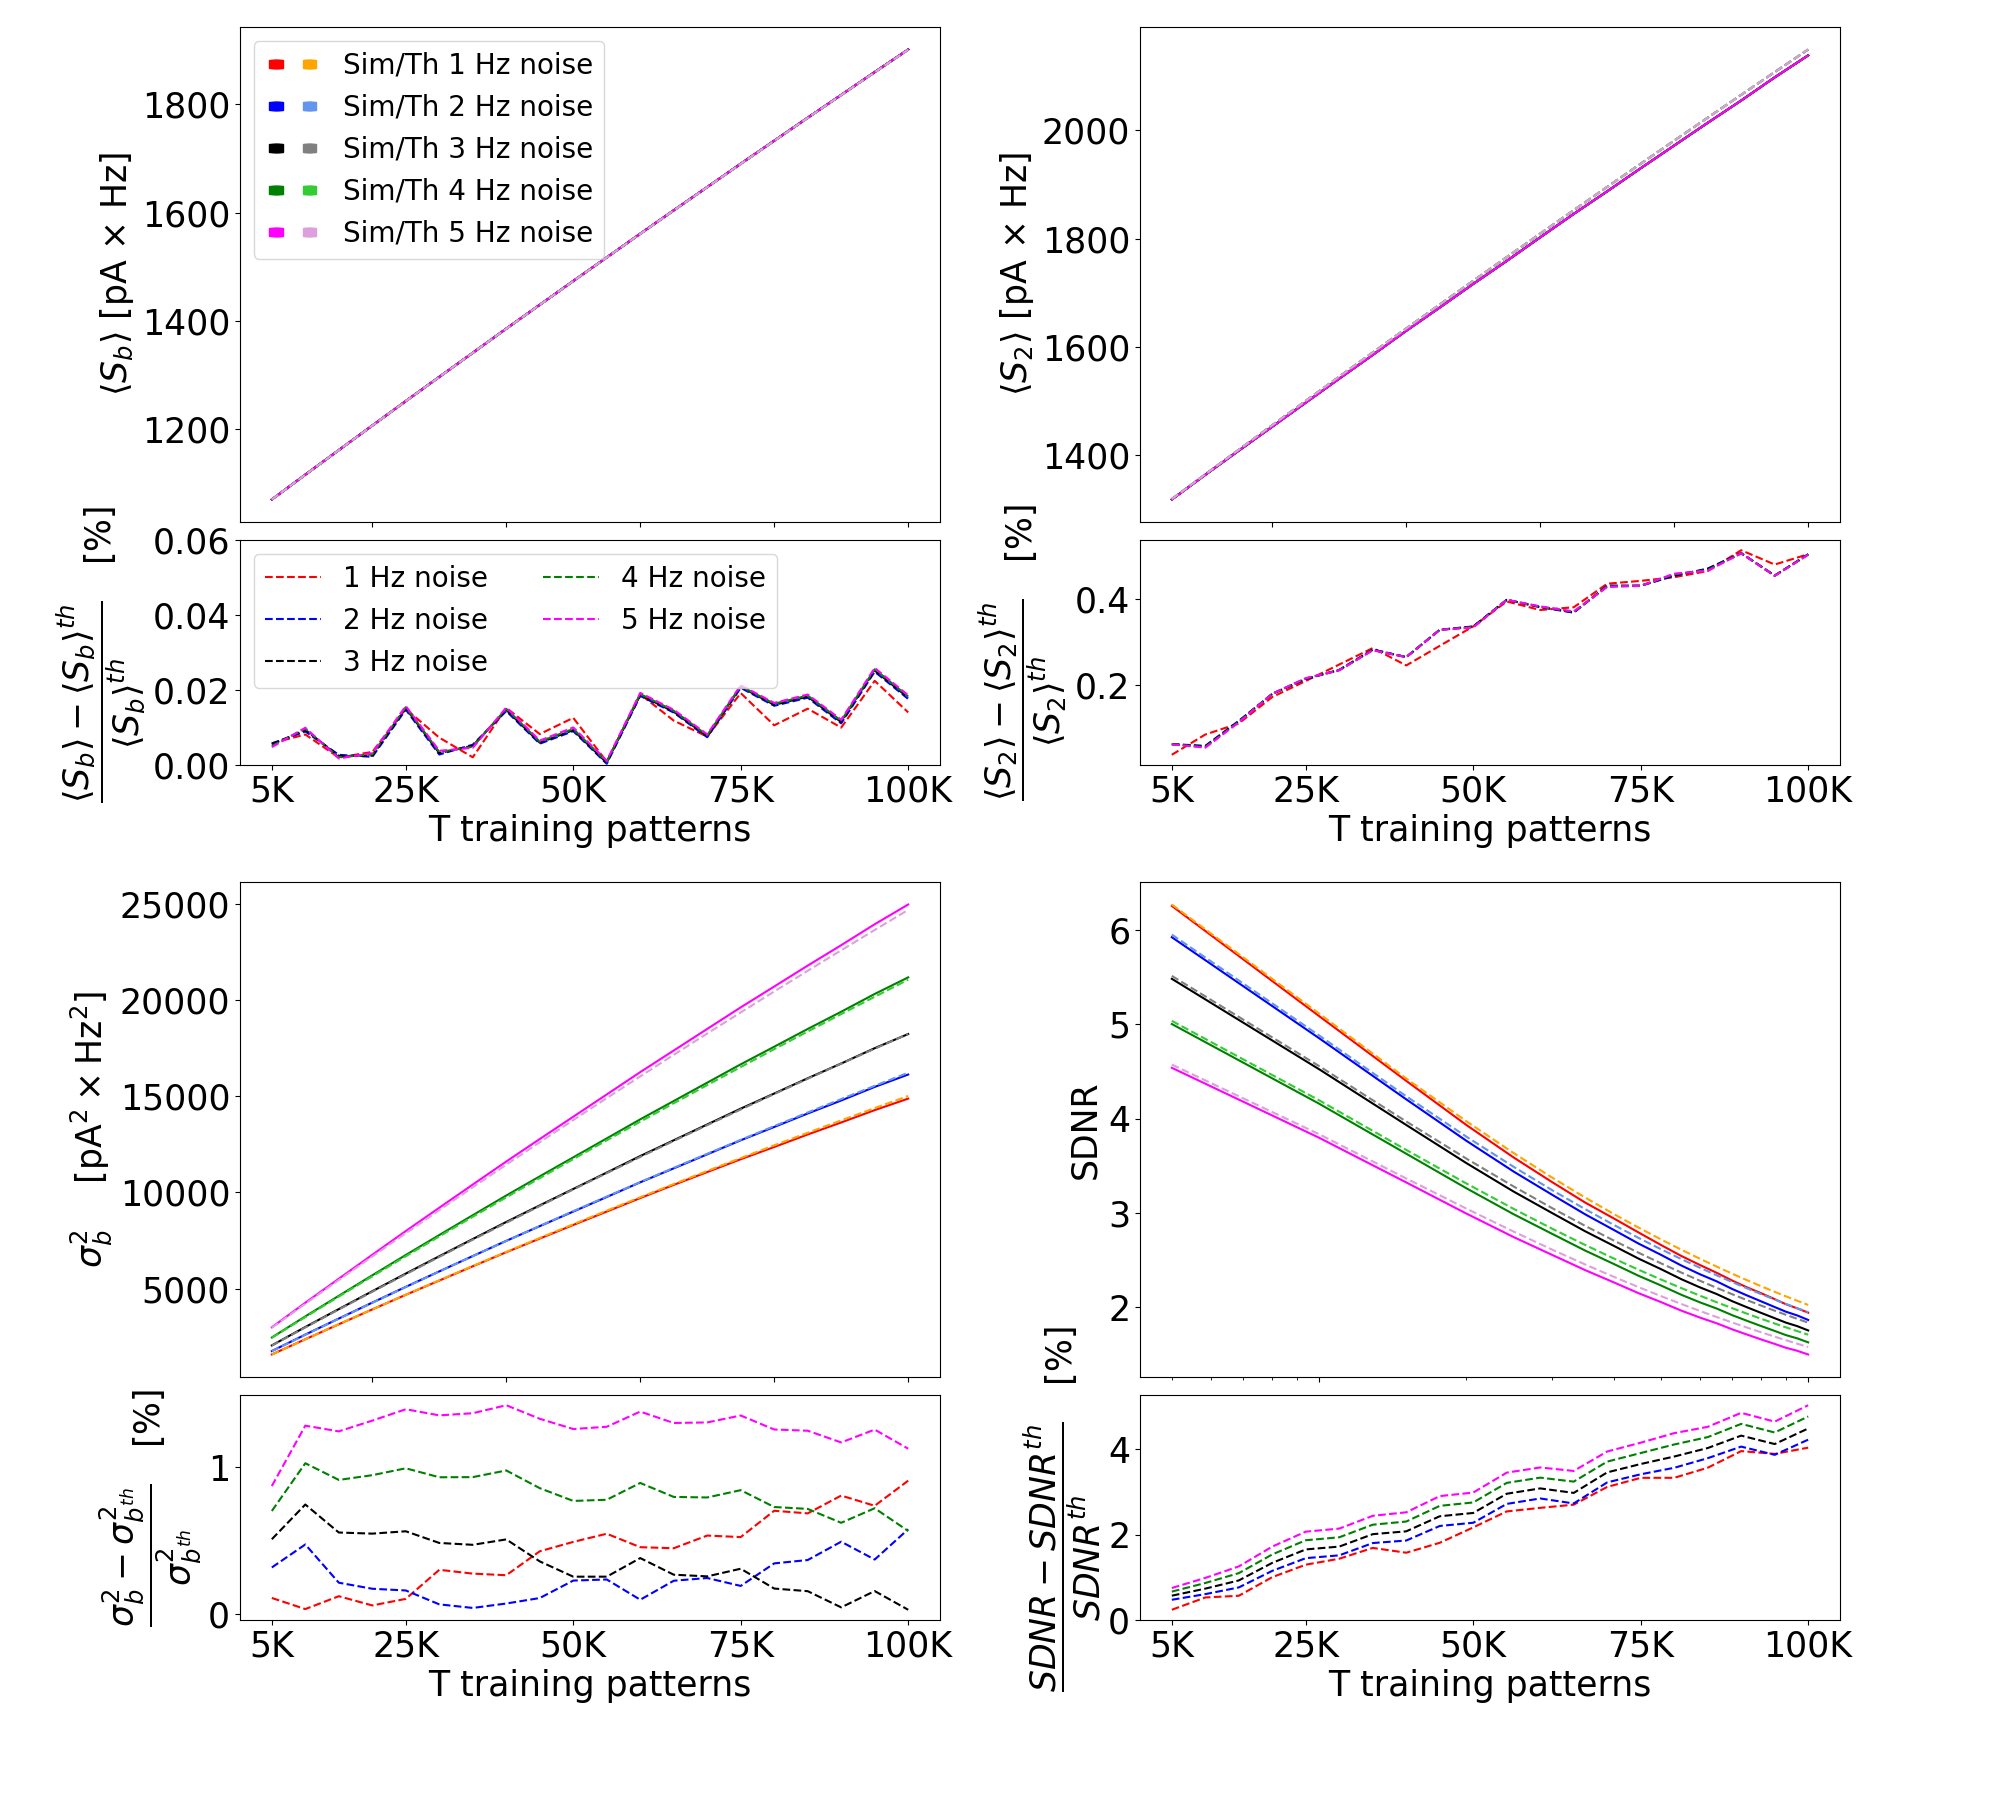
\includegraphics[width=\columnwidth]{figures/lognormal.png}
\caption{Values of $\langle\Sb\rangle$, $\langle\SII\rangle$, $\varSb$ and the SDNR and percent error with respect to the theoretical prediction, as a function of the number of training patterns $\T$. 
Bigger subplots represent the values of the quantities considered as a function of $\T$ for different noise levels, whereas each smaller subplot represent the percentage error of the values shown in the upper subplot. The different color families identify the simulation and theory results when having a noise standard deviation of $1$\,Hz (red-orange), $2$\,Hz (blue-light blue), $3$\,Hz (black-grey), $4$\,Hz (green-light green) and $5$\,Hz (magenta-pink).
\label{fig:relative-error}}
\end{figure}

As described previously, the test input patterns used in the continuous rate model are altered from the corresponding training input patterns by adding noise extracted from a truncated Gaussian distribution, with assigned standard deviation. In this section, we present simulation results and comparisons with theoretical predictions for standard deviation values ranging from $1$\,Hz to $5$\,Hz.
These values are relatively high in relation to the average firing rate of $\popI$, which is slightly higher than $2$\,Hz.\\
Figure \ref{fig:relative-error} shows the curves obtained for the continuous rate model using different values for the standard deviation of the noise, together with the relative error with respect to theoretical predictions.

It can be observed that the curves obtained from the simulations are compatible with the theoretical ones for all the noise levels.


Regarding $\langle\Sb\rangle$ and $\langle\SII\rangle$, the curves corresponding to different noise levels appear perfectly superimposed.
This is due to the fact that the noise is driven by a distribution with zero mean, and thus the addition of noise to the quantities represented in the curves does not alter their average (see Appendix \ref{app:noise} for the details). Regarding $\varSb$, the values corresponding to
different noise levels
differ from each other and increase with the standard deviation of the noise, in agreement with the theoretical model.\\
The relative error between simulation results and theoretical prediction is quite small: for $\langle\Sb\rangle$ and $\langle\SII\rangle$ the errors span between $0.01$\% and $0.4$\%, whereas $\varSb$ shows a relative error of around $1$\% for all the simulations performed with different number of training patterns.


The addition of noise with fluctuations greater than or comparable to the average firing rate can
produce negative rate values for a fraction of the neurons.
Considering that negative rate values are not physically possible, this behavior can be corrected in the simulations by simply  replacing negative values of the firing rates with zero, i.e. saturating negative rates
to zero.
This correction is equivalent to having a different noise distribution, with an average value greater than zero.
However, the current theoretical model is not able to take this effect into account. Since negative values are replaced by zeros,
we would expect the average values of $\Sb$ and $\SII$ evaluated by the simulations that exploit saturation to be greater than the values
predicted by the theoretical model.
Figure \ref{fig:relative-error-saturation} shows the behavior of the model with this correction on the neurons firing rate.



As can be seen from the figure, the discrepancies between simulations and theoretical predictions are much higher and can arrive to $40$\%. This is due to the fact that the current theoretical framework is not able to take this correction into account.
However it should be considered, as discussed above, that the considered noise levels are relatively high when compared with the average rate used in these simulations.
Indeed, a different choice for the values of $\langle \rl \rangle$ and $\langle \rh \rangle$ (and thus a different average rate of the whole distribution) would have an impact on the discrepancies shown here.
In particular, a higher average rate would strongly diminish the amount of neurons having
negative firing rate as a result of the noise addition.

The relative error of $\varSb$ is greater than that shown for $\langle \Sb \rangle$ and $\langle \SII \rangle$ in Figure \ref{fig:relative-error}; this is due to a simplification used in the theoretical model to derive the expression of the variance.
The values of $\Sb$ from which we compute the variance are obtained by incoming connections 
from neurons of $\popI$, but since connections are created randomly, different neurons of the $\popII$ population may have presynaptic neurons in common, and therefore their input signals are correlated.
The theoretical model does not take this correlation into account.
The average number of presynaptic neurons in common to two arbitrary neurons of
$\popII$ depends on the total number of neurons of $\popI$ and on the number of incoming connections per neuron of $\popII$.

\begin{figure}[H]
\centering\includegraphics[width=\columnwidth]{figures/lognormal_saturation.png}
	\caption{ 
	Values of $\langle\Sb\rangle$, $\langle\SII\rangle$, $\varSb$ and SDNR, and percent error with respect to the theoretical predictions, as a function of the number of training patterns $\T$ when negative rates due to noise addition are saturated to zero.
    The different color families identify the simulation and theory results when having a noise standard deviation of $1$\,Hz (red-orange), $2$\,Hz (blue-light blue), $3$\,Hz (black-grey), $4$\,Hz (green-light green) and $5$\,Hz (magenta-pink).
	\label{fig:relative-error-saturation}}
\end{figure}

Calling $\NI=\mathcal{N}$, we can state that the bias due to this simplification becomes more and more relevant when the ratio $\mathcal{C}/\mathcal{N}$ increases.
In order to estimate this bias as a function of the $\mathcal{C}/\mathcal{N}$ ratio,
we performed a series of simulations with a fixed
number of training patterns, $\T=5000$, changing the $\mathcal{C}/\mathcal{N}$ ratio.
Figure \ref{fig:c_n_comparison} shows the results of this analysis.

\begin{figure}[t]
    \centering
	\includegraphics[width=\columnwidth]{figures/cn_plot.png}
	\caption{ 
    Values of $\varSb$ as a function of the $\mathcal{C}/\mathcal{N}$ ratio for different values of $\mathcal{N}$. On left panel, lines represent the theoretical prediction (Th), whereas dots represent the values obtained from the simulation (Sim). On the right panel, dotted lines represent the relative error between simulation results and theoretical prediction.
	\label{fig:c_n_comparison}}
\end{figure}

As can be seen in the right panel of Figure \ref{fig:c_n_comparison}, a greater value of $\mathcal{C}/\mathcal{N}$ leads to a higher discrepancy between theoretical prediction and simulation. However, such a ratio, for natural density circuits in the brain, is very far from values of $\mathcal{C}/\mathcal{N}$ near unity. Indeed, a plausible value of the ratio would be less than $0.1$, resulting in negligible relative errors.


\subsection{Impact of synaptic rewiring}
In the simulations discussed so far, the rewiring mechanism was always performed with
a rewiring step $s=100$.
This means that every $100$ training patterns,
all the unconsolidated connections are removed, and new connections are created.
This operation represents the effect of homeostatic structural plasticity, that aims at keeping the network balanced by reorganizing connections, while activity-dependent structural plasticity focuses on the consolidation of connections.\\
To motivate the choice of this step for connection rewiring, we show here the results for networks trained for $\T=5000$ patterns with a different rewiring step $s$.
We also show the results of a simulation that does not perform rewiring, in order to highlight
the different behavior of a network that combines connection consolidation with periodic rewiring and that of a network that exploits only connection consolidation.
Figure \ref{fig:t_study} shows the results obtained by these simulations using different rewiring intervals. 

\begin{figure}[t]
    \centering\includegraphics[width=\columnwidth]{figures/t_study.png}
	\caption{ 
    Values of $\langle\Sb\rangle$, $\langle\SII\rangle$, $\varSb$ and SDNR
    for a network trained with $5000$ patterns as a function of the rewiring step $s$. 
    The simulations used a continuous rate distribution and a noisy input driven by truncated Gaussian distribution with standard deviation of $1$\,Hz. The red dot indicates the simulation outcome when connection rewiring is disabled, whereas the blue line shows the simulation results with connection rewiring, using different values of $s$. Blue shading represents the standard deviation of the mean obtained from $10$ simulations using different seeds for random number generation.
	\label{fig:t_study}}
\end{figure}

As can be noticed, the values of $\Sb$, $\SII$, $\varSb$ and SDNR do not change significantly as the rewiring step varies.
This means that the value of the step $s$ chosen for the connection rewiring has no impact in the results of the simulations.
On the other hand, significant differences emerge when comparing the results of simulations
with or without connection rewiring; it can be observed that the signal-difference-to-noise ratio has a lower value  when the rewiring is disabled. This confirms that connection rewiring grants a higher capability of recognising an input pattern among the several patterns
for which the network was trained.\\
We also applied a similar protocol for simulations enabling or disabling connection rewiring as a function of the number of training patterns $\T$. The results are shown in Figure \ref{fig:rew_vs_norew}.\\
We can say that the performance of the model are improved when connection rewiring is enabled, and the relative difference between a rewired or just consolidated connectivity increases when increasing the number of training patterns.\\
The effect of rewiring can become more relevant when a greater number of connections is consolidated at every step (i.e., with greater values of $p_1$ and $p_2$).
Furthermore, the importance of the rewiring mechanisms can significantly change 
when the average number of connections is not constant, but increases or decreases as a result of rewiring itself. This aspect will be explored in a future work.

\begin{figure}[t]
    \centering
	\includegraphics[width=\columnwidth]{figures/no_rewiring.png}
	\caption{ 
    Comparison between simulations exploiting the
    connection rewiring mechanism performed every $100$ training patterns (blue lines) and simulations without rewiring (red lines) for a network trained with a variable number of training patterns $\T$. Green lines in the sub-panels show the difference between the values obtained with connections rewired or not rewired (indicated with $nr$) as percentage error.
	\label{fig:rew_vs_norew}}
\end{figure}



\fancyfoot[C]{\thepage}
\fancyfoot[L]{Gianmarco Tiddia}
\fancyfoot[R]{Discussion}

\part*{Discussion}
\addcontentsline{toc}{part}{Discussion}

This thesis covers several aspects of computational neuroscience, from simulation technology to a better understanding of the synaptic mechanisms underlying high-level cognitive processes. To better organize the discussion of the results presented in this thesis, different topics are presented in different sections.

\section*{GPU-based simulations using NEST GPU}
\addcontentsline{toc}{section}{GPU-based simulations using NEST GPU}
In Part \ref{part:I} of this thesis we focused on the simulation of spiking networks accelerated by the GPU simulation code NEST GPU. In the context of this thesis, we implemented network models such as the cortical microcircuit of \cite{Potjans2012} and the multi-area model of \cite{Schmidt2018,Schmidt2018b} and we validated the results of the network activity with the ones of the spiking network simulator NEST through the comparison of some relevant statistical distributions. The validation protocol is described in Chapter \ref{chapter:models_and_validation} and the results of the validation of these models are shown in Chapter \ref{chapter:comparison_NEST_NGPU}, showing optimal compatibility between NEST GPU and NEST. In particular, the validation protocol aims to perform a statistical comparison between the fluctuation in some distributions of the spiking activity, which have been employed in several other works (see, for example, \cite{VanAlbada2018, Knight2018, Dasbach2021, Heittmann2022}).
First, the fluctuations within NEST simulations (i.e., when different seeds for random number generation are employed) and with NEST and NEST GPU are evaluated. A comparability of these fluctuations would lead to the conclusion that the simulation on a different simulator does not add additional variability in the simulation of the neural activity. The results shown in Chapter \ref{chapter:comparison_NEST_NGPU} show an optimal compatibility with the statistical distributions of the neural activity of NEST, both in the simulation of the cortical microcircuit model and in the simulations of the multi-area model. This is a theme of fundamental importance for better integration of NEST GPU in the software of the NEST Initiative. Indeed, this work focuses also on the integration of neuron, synapse models and connection rules already integrated in NEST. Furthermore, to enable the users to take advantage of all the features of the library, a documentation similar to the one of NEST has been written and periodically updated.\\
Another relevant topic is the evaluation of the performance of NEST GPU. To better study the different simulation stages, we divided the total time-to-solution into two phases: network construction (i.e., the time needed to create and organize the network before the simulation of the dynamics) and simulation (i.e., the actual simulation of the network dynamics). Indeed, these phases can be further divided into different stages, as described in Chapter \ref{chapter:performance_evaluation}. Regarding network construction time, this thesis and \cite{Golosio2023} presented a novel algorithm for network construction, which dynamically creates the network exploiting the high degree of parallelism of GPU devices. In the first version of the library (see \cite{Golosio2021}), connections were first created on the CPU side and then copied from the RAM to GPU memory. This approach benefited from the standard C++ libraries and, particularly, the dynamic allocation of container classes of the C++ Standard Template Library. However, it had the drawback of relatively long network construction times, not only due to the costly copying of connections and other CPU-side initialization, but also because the connection creation process was performed serially. The new approach, so far applied to single-GPU simulations, enables much faster connection creation, initialization, and organization while preserving the advantages of dynamic connection building, particularly the ability to create and initialize the model at run-time without the need for compilation. With the current version, it is possible to construct a network such as the cortical microcircuit model of \cite{Potjans2012} in around half of a second, two orders of magnitude less than the previous method. Comparing this result with other simulation codes, NEST GPU network construction times are also shorter compared to the CPU version of NEST and the code generation framework GeNN (see Figure \ref{fig:network_construction_ngpu_nest_genn}); if code generation and compilation are not required in GeNN, the results of NEST GPU and GeNN are compatible. We also verified that the time to simulate the network dynamics after network construction is not compromised by the novel approach. Regarding the network dynamics, in Figure \ref{fig:cm_rtf_old_new} it can be observed the improvement in the simulation of the full-scale cortical microcircuit model of \cite{Potjans2012} between the first version of the GPU library (i.e., NeuronGPU \cite{Golosio2021}) and the most recent version of the library employed in \cite{Golosio2023} using both data center and consumer GPUs. We can notice that the optimization performed on the library on many aspects of the code led to an improvement in the simulation performance spanning from $55\%$ to $75\%$ depending on the GPU hardware employed. In particular, the best result is achieved with the NVIDIA RTX 4090, with a real-time factor, averaged over 10 simulations with different seeds, of $0.4707\pm 0.0008$ \cite{Golosio2023}. This result is obtained with the external drive of the model being a Poisson signal generator, however, Figure \ref{fig:cm_overall_RTF} shows the real-time factor when a DC input is given to the network instead of the Poisson stimulation, obtaining a real-time factor of $0.386\pm 0.001$ when employing the same GPU. We can thus notice that in both the configurations, NEST GPU can perform sub-realtime simulation of this model, even outperforming the CPU simulator NEST in an optimal parallelization configuration (see Figure \ref{fig:cm_overall_RTF}A and \cite{Kurth2022} for additional details). Moreover, the same Figure shows the results for the simulation of the same model performed using the GPU code GeNN (version 4.8.0), which mimics the incoming Poisson spike trains via a current directly applied to each neuron. Thus, the implementation of the external stimulation is not the same as the one of NEST or NEST GPU. However, it can be seen that GeNN currently simulates faster than NEST GPU. Indeed, this indicates that there is room for improvement, which could be exploited via further parallelizations of the simulation kernel of NEST GPU. Moreover, the algorithm for runtime network construction directly on GPU devices is being extended in order to be exploited into multi-GPU simulations. This would lead to a further increase in NEST GPU performance on network construction for large-scale models that have to be simulated on MPI-GPU clusters.\\
Indeed, NEST GPU was also designed to perform an efficient algorithm for spike delivery and communication across different compute nodes via MPI-GPU clusters. Moreover, NEST GPU distributes neurons across MPI processes exploiting their locality, i.e., an entire neuron population is created and simulated on a single MPI process, to be specified by the user.
In this regard, in \cite{Tiddia2022} we validated NEST GPU with the simulation of the multi-area model of \cite{Schmidt2018,Schmidt2018b} describing the dynamics of the vision-related areas of the macaque cortex. The results of the validation (see Chapter \ref{chapter:comparison_NEST_NGPU} and Appendix \ref{app:mam_validation}) show optimal compatibility with the results obtained with the NEST simulator, both for the ground and in the metastable state of the model. Moreover, Figure \ref{fig:mam_benchmark} shows the real-time factor of the CPU and GPU code of NEST in both the ground and metastable state, noticing that the locality exploitation of NEST GPU is one of the major contributors to the better performance of NEST GPU with respect to NEST, in which neurons are distributed in a round-robin fashion. Indeed, both these approaches show advantages and disadvantages: in NEST every MPI process handles the same amount of compute load, whereas in NEST GPU the compute load differs (see for example Figure \ref{fig:mam_relative_contrib_sim_time}). However, in the case of the multi-area model, the locality exploitation is a more efficient approach since the vast majority of the spikes emitted in a simulation of the network is exchanged between neurons belonging to the same area, i.e., the same MPI process according to the NEST GPU approach. This way, only a fraction of the spikes have to be delivered remotely. 
In summary, NEST GPU is able to perform simulations of spiking networks taking advantage of both data center and consumer GPUs. The library grants network construction times comparable to or shorter than those obtained with other state-of-the-art simulation technologies while still meeting the flexibility of runtime network construction. The library is able to take advantage of multi-GPU systems and thanks to an efficient algorithm for spike delivery and network locality exploitation, it is particularly suitable in the simulation of modular large-scale models that can not be simulated on a single GPU card.\\
To be thorough, in \cite{Knight2021b}, it is shown that GeNN was able to simulate the multi-area model previously mentioned on a single GPU by exploiting the procedural connectivity approach mentioned in Chapter \ref{chapter:intro_simulators}. With this method, the network generates the network connectivity on the go, without saving data on the GPU memory and thus being able of simulating a larger network on a single card. However, such a network would not be suitable when plastic connections have to be employed, thus is not applicable in cases in which learning or the interplay between synaptic changes and brain dynamics are of interest (e.g., in \cite{Capone2019,Golosio2021-ThaCo,DeLuca2023}).\\


Without any doubt, NEST GPU has room for improvement in several aspects, from additional optimization of the simulation phase (e.g. increasing the level of parallelization of several subtasks) to further integration of the library into the NEST Initiative. A further alignment to the NEST simulator is needed to enable the same code to be run on both the CPU and GPU simulators, and also additional neuron, synapse models and connection rules have to be implemented on NEST GPU to have an appropriate variety and flexibility. Moreover, the support of NESTML, a domain-specific language that allows the modification or the creation of neuron or synapse models, would be fundamental for implementing new models in a simple format. In addition, to fully benefit from the features of the library, an updated documentation is needed to guide the user in the choice of the most appropriate neuron, synapse models and parallelization approaches.


Finally, from a general perspective, recent advancements in GPU technology and the development of exascale MPI-GPU clusters would surely contribute to an increase in the performance on the simulation of large-scale spiking network models, but most importantly would open to the development of even larger network models, with several millions of neurons and billions of synapses. In this regard, with NEST GPU we provided a tool able to exploit the most recent technology, paving the way for more and more detailed network models, that could be able to explore, with a neuron resolution, the dynamics of brain networks handling high-level cognitive processes. 

\section*{Short-term plasticity and working memory}
\addcontentsline{toc}{section}{Short-term plasticity and working memory}

In Part \ref{part:II} of this thesis we focused on the study of synaptic mechanisms underlying cognitive processes. In Chapter \ref{chapter:STP_WM_model} we present a spiking network model able to show a typical working memory behavior only by implementing short-term synaptic plasticity in the excitatory-to-excitatory synapses. The hypothesis of a synaptic theory of working memory was initially presented in the work of Mongillo \cite{Mongillo2008}, together with the simulations of a spiking network that we reproduce in the context of this thesis to provide a well-documented spiking model implemented on a widely used spiking network simulator (i.e., NEST). To this aim, we edited the implementation of the short-term plasticity model of NEST (more details on Appendix \ref{app:STP_implementation}) and we propose a similar network model based on the instructions provided in the original work. Despite some differences in the implementation and in the value of the parameters, we were able to correctly reproduce the results of \cite{Mongillo2008}, and we were also able to estimate the working memory capacity according to the work of \cite{mi_katkov_tsodyks2017}, in which a similar network model was employed to estimate the working memory capacity as a function of synaptic and neuron parameters. As discussed in \ref{sec:WM_STP_discussion}, this work aims to pave the way for further studies on the relation between synaptic processes such as short-term plasticity and working memory. In this regard, such studies can shed light on the mechanisms that contribute to high-level cognitive processes.


Furthermore, the model reproduced in this thesis, in which the only ingredient to obtain a memory-specific response is an STP-modulated synaptic efficacy and prior long-term Hebbian learning, has several limitations. For instance, the previously mentioned prior learning process is needed, and the synapses can assume only two values of absolute synaptic efficacy (i.e., $J_b$ or $J_p$). A more realistic network would implement a proper training protocol in order to mimic a realistic learning process, with connections having heterogeneous synaptic strengths. Additionally, the STP variables $u$ and $x$ have the same initial values for all the connections of the network. An interesting work would thus add heterogeneity to synapse parameters, from synaptic weights to STP time constants and variables, to provide the results of a more realistic network able to underlie working memory. Indeed, a study related to a different model relying on persistent activity, revealed that heterogeneity in neurons and synapse parameters is able to prevent the appearance of persistent activity \cite{Hass2022}, showing that persistent activity regime can be restored when some compensating mechanisms are added (e.g., homeostatic synaptic plasticity, an increase in the number of neurons or in the external input). A similar study can thus be interesting for our model, in particular adding heterogeneity to synaptic efficacies and STP parameters.


Another limit of the model reproduced in this thesis is related to the fact that once the network enters the regime of persistent population spikes or higher-rate activity (see panels B and C of Figure \ref{fig:figure2}) it can return to the lower activity state only with a decrease of the background current. Thus, for such an activity to have a selected duration, another mechanism has to be added to the network. Recent work of \cite{DePitta2022} suggests that, together with neurons, astrocytes can modulate neural activity. Thus, interactions between glia and synapses contribute to synaptic transmission and can underlie multiple forms of working memory. Another interesting work on astrocytes involved in working memory was able to show that astrocytic mechanisms are involved in the duration modulation of the persistent activity state \cite{Becker2022}. In particular, this work employed the model of Mongillo \cite{Mongillo2008} with the addition of an astrocytic mechanism with a proper time constant and a parameter that influences the calcium dynamics described by the variable $u$. This way the network is able to show the population spike or the high-asynchronous activity regime for a limited time, determined by the dynamics of the astrocytic mechanism. 


As we can see, the quest to account for synaptic mechanisms in working memory is leading to several models in which many processes should be taken into account to better model a high-level cognitive process such as working memory. Indeed, the synaptic theory of working memory suggests that activity-silent processes take place to encode chunks for a limited time, whereas the theory proposed at the beginning relied on persistent activity as the key mechanism underlying working memory. Several experimental findings support both these hypotheses, and the idea that both regimes coexist has also been proposed \cite{Masse2019, Kamiski2019}. Novel experiments will be needed to shed light on the neural and synaptic mechanisms underlying this high-level cognitive process, and more detailed computational modeling of different processes that can contribute to working memory will be of fundamental importance to flank experiments and provide tools to further analyze the impact of these mechanisms in working memory.


\section*{Structural plasticity and learning}
\addcontentsline{toc}{section}{Structural plasticity and learning}

The last chapters of Part \ref{part:II} presented a theoretical framework for learning through a structural plasticity mechanism, described also in \cite{Tiddia2023}. The predictions of the theoretical framework, based on a mean-field approach, have been compared with the results of simulations performed using firing-rate-based neuronal networks.
The comparison shows that the proposed framework is able to accurately predict the values of various quantities relevant for assessing learning and memory capacity in the presence of structural plasticity mechanisms, taking into account numerous characteristics of biological neuronal networks.
The rates of neurons in the training and test patterns can be distributed according to an arbitrary probability distribution. Here, two cases have been considered: a simplified one in which the rates can assume only two values, high rate and low rate, and a more realistic one in which the rates follow a log-normal distribution in agreement with \cite{Roxin2011}.
Connectivity between regions can be achieved through different connection rules, with a fixed number of connections per target neuron or, more realistically,
with random connectivity in which the number of incoming connections of each target neuron follows a Poisson distribution.\\
Since the biochemical and biophysical mechanisms underlying structural plasticity are multiple and extremely complex, we opted for a phenomenological approach to capture their main aspects. This way, we exploited a simple model of structural plasticity able to represent plasticity processes driven by neuronal activity as well as mechanisms that leads to homeostasis, in agreement with \cite{Fauth2016}, which divides structural plasticity mechanisms into these two categories.
Structural plasticity driven by neuronal activity is achieved through the consolidation of synapses connecting neurons that are concurrently at a high-rate level.
This process can be triggered by other forms of plasticity that modify synaptic efficacy, such as STDP, followed by 
mechanisms involving cytoarchitectural changes, such as the creation of novel connections next to the already existing ones.\\
The homeostatic form of structural plasticity involves a balance between pruning connections that are not utilized over time and the creation of novel connections.
This is achieved in the simulations through periodic connection rewiring, which consists of a removal of unconsolidated connections followed by the creation of new connections.
The results show that connection rewiring leads to an increase in SDNR, conducting to a higher capability of recognizing the input patterns when this mechanism is enabled.\\
In order to evaluate the generalization capability of the framework with the continuous firing-rate distribution model, the test patterns were generated by altering the training input patterns through the addition of noise from a given probability distribution and assigned standard deviation. In particular, a truncated Gaussian distribution has been used for the noise.
The results of the simulations are compatible with the theoretical predictions, with differences in the order of $1-2$\%, which is a remarkable result for our purpose.\\
However, such an approach can lead to a fraction of the neurons with a negative firing rate as a result of noise addition. Since negative firing rates are not physically possible, a more realistic model would apply a saturation to zero for these rates. Saturation can be activated in the neuronal network simulations, but the current version of the theoretical framework is still unable to account for it. This leads to a discrepancy between the simulations with saturation turned on and the theoretical predictions, which grows as the noise increases and becomes relevant when the noise gets significantly greater than the average firing rate.
Future work on this model should be devoted to the development of a theoretical framework capable of taking into account the saturation of negative firing rates.\\
Another limitation of the framework comes from a simplification in the calculation of the background signal variance, which does not take into account the correlations between the contributions of presynaptic neurons to the input signals to distinct neurons of the target population.
However, the results show that the impact of this simplification is very small, at most in the order of a few percent.


The theoretical model can be surely extended. It can potentially provide a powerful tool to describe the impact of structural plasticity in cognitive processes such as learning in a large-scale model of the cortex with natural density and plausible characteristics. For instance, the consolidation mechanism can be probability-driven, with a probability depending on the rate of pre- and postsynaptic neurons. This would replace the current deterministic mechanism that requires a firing rate threshold to be exceeded by both neurons to have synaptic consolidation. Moreover, the probability could depend on other variables not necessarily related to the firing rate.
In particular, it has been hypothesized that plasticity mechanisms may also depend on the bursting activity of neurons \cite{Butts2007, Payeur2021}.
The consolidation probability of a connection could therefore depend, in addition to the firing rate of the presynaptic and postsynaptic neurons, also to their bursting activity. In this regard, it would be interesting to expand this work through simulations of spiking neural networks. Indeed, simulators such as NEST \cite{NEST} and its GPU implementation \cite{Tiddia2022, Golosio2023} can lead to fast and efficient simulations of large-scale models on supercomputer clusters.


In Chapter \ref{chapter:structural_plasticity_theory} we have mainly considered the connections between two distinct populations $\popI$ and $\popII$. However, the proposed framework also lends itself to the study of structural plasticity in the self-connections of population $\popII$, together with an inhibitory population in order to have a more realistic architecture of excitatory and inhibitory neurons. Indeed, it is known that the mechanisms of competition through lateral inhibition play a key role in biological learning \cite{Coultrip1992}. Section \ref{sec:recurrent_model} of this thesis is devoted to the description of such a recurrent network model. In this extended model, the theoretical framework allows to obtain the differential equations governing the dynamics of the activity of the population $\popII$ and the dependence of the coefficients of these equations on the number of training patterns and on the other model parameters \cite{Sergi2023}. Such an extension is currently under development and additional work has to be done to provide an extensive description of all the features of this model and for an appropriate choice of simulation parameters.


Another extension of the model could describe more in detail the mechanisms of synaptic pruning and rewiring. Indeed, connection rewiring as intended in the feed-forward model preserves the total number of connections over time, which is a typical behavior of a healthy adult brain \cite{Huttenlocher1979}. However, to shed light on the importance of this mechanism in neurological disorders, or to perform studies focused on this mechanism in different life stages, this mechanism should be extended to enable different "speed" for the processes embedded in structural plasticity.\\


In conclusion, this work intends to provide a sufficiently general theoretical framework for learning through structural plasticity. This framework is able to describe synaptic consolidation, pruning and rewiring, and includes several features that can be added in a modular fashion.
The validation has been performed through simulations with firing-rate-based neuronal network models, showing remarkable compatibility between the results of the simulations and theoretical predictions.


\section*{Outlook}
\addcontentsline{toc}{section}{Outlook}

This thesis makes several contributions to computational neuroscience, with a particular focus on simulation technology and the understanding of synaptic mechanisms in high-level cognitive processes.

Chapters \ref{chapter:intro_simulators}-\ref{chapter:performance_evaluation} are devoted to the validation of a new simulation code (i.e., NEST GPU) able to exploit the most recent GPU technology advancements. Indeed, GPUs, with their high degree of parallelism, are particularly suitable to handle the simulation of spiking neural networks and the rapid growth of the GPU industry is leading to more performing cards and, most importantly, gradual improvements in the GPU memory. Moreover, supercomputers are entering the exascale era and entrust GPUs with a significant part of their computing power. In this framework, a simulator able to take advantage of this technology is fundamental to open to more detailed simulations of the neuronal dynamics of large-scale networks. Most importantly, this simulator should be easily accessible to the neuroscientific community and the compatibility of the results with respect to affirmed and widely used simulators should be ensured. In this context, the integration of the simulator in the NEST Initiative and the work performed in \cite{Golosio2021, Tiddia2022, Golosio2023} go in this direction, by assessing the compatibility of NEST and NEST GPU for different models running both on high-end PCs and MPI-GPU clusters with competitive simulation performance both on network construction and simulation of the network dynamics.


Chapters \ref{chapter:STP_WM_model}-\ref{chapter:structural_plasticity_simulation} focuses on two synaptic mechanisms that are able to underlie high-level cognitive processes: short-term synaptic plasticity and structural synaptic plasticity. The works described in this thesis can be intended as starting points for future works devoted to clarifying the relationship between these mechanisms and brain functioning. The first of the two aforementioned chapters analyzes the relation between short-term plasticity and working memory through spiking network model simulations, whereas the second sheds light on the role of structural plasticity during learning through a theoretical framework based on a mean-field approach supported by simulations of firing-rate based neuronal networks.


In conclusion, this thesis aims to provide the instruments needed to face the challenge of the study of high-level cognitive processes through simulations of large-scale neuronal networks. In the near future, simulation codes such as NEST GPU will be able to simulate network models of substantial portions of the brain that have never been studied on a single neuron scale, and a better understanding of the role of synaptic scale mechanisms will be needed to evaluate their impact on such a large-scale perspective, or the impact of their inhibition. In this regard, neural scale simulation frameworks could be seen as virtual tools able to be employed for testing novel treatments or to evaluate the large-scale effect of a drug able to affect a certain brain mechanism. For this reason, it is fundamental to benefit from the novel technological progress and pave the way for an era in which computational neuroscience can develop network models and theoretical frameworks able to flank experiments and advance our knowledge of brain functioning.


\fancyfoot[C]{\thepage}
\fancyfoot[L]{Gianmarco Tiddia}
\fancyfoot[R]{}

\bibliography{bibliography.bib}
\bibliographystyle{ieeetr}


\newpage
\null
\thispagestyle{empty}
\newpage
\chapter*{Acknowledgements}

I am deeply grateful to all those who have contributed to the successful completion of this thesis\footnote{including myself}. Their support and guidance have been invaluable throughout this research journey.

First and foremost, I extend thanks to my supervisor, Bruno Golosio, for his support, expert guidance, and invaluable mentorship not only for the PhD, but for my whole academic path. Your dedication to my academic and professional growth has been fundamental, and I think a simple acknowledgement section wouldn't be enough to express my gratitude. I would also like to express my sincere thanks to Pier Stanislao Paolucci, my co-supervisor, for his insightful feedback and support.

I want to thank the rest of NEST GPU team for the continuous collaboration during these years. In this regard, a special thank goes to Jose, for his support during my stay in Germany and for the fruitful collaboration that led to the totally-doable-within-March work (i.e., \cite{Golosio2023}, submitted in June) and for all the time spent together first remotely and then in person, especially when discussing the questionability of pineapple pizza.

A special thank goes also to the ones that made my period abroad just great. First of all, I want to thank Tom for his supervision and the numerous insights, and together with him I want to deeply thank Markus, Johanna, Melissa, Anno and Jasper for welcoming me into their group, in which I spent one of the best times of my PhD.

Coming back to Cagliari, I want to deeply thank my PhD colleagues and Luca Sergi for sharing lunches, coffees and lots of nonsense. Without you all, I wouldn't have been able to bear all the stress of these years, and I hope I helped you as well as you all helped me to get this far. In particular, I want to thank my office mates Camilla and Riccardo for all the time spent supporting each other, and, last but not least, Nicola. We started together as Bachelor students, we continued as Master students and we ended up as office mates during the PhD. I hope this is not the last time for us to work side by side, also because we share a coffee machine and cannot split it into two working parts. However, I am sure that even if things do not go as we hope, our friendship will stand the test of time. I thank also Nicola Deiosso and Luca Delussu; although our paths parted some time ago, we have always stayed in touch by supporting each other and giving each other advice.

Tightening up the circle, I want to thank my longtime friends, starting from Federico, Giacomo, Nicola, Fabio, Daniele, Luca (Manca), Jacopo and ending with Alessandro, Matteo and Luca (Spada). Our friendship lasts for as long as I can remember and I am grateful that, despite we took different life paths over the years, we can always count on each other.

I would also like to express my deepest gratitude to someone who has been my constant source of support, encouragement, and love: my girlfriend Sara. Your presence provided me with enough balance to navigate the challenges of this endeavor and, as you like to tell, you brought colors into my grey-scale life. Thanks to you, I can say that I'm happily RGB.

Last but not least, I thank my parents for their constant support during these years.









\appendix

\fancyfoot[C]{\thepage}
\fancyfoot[L]{Gianmarco Tiddia}
\fancyfoot[R]{Appendix}

\chapter{Additional information for the balanced network model}
\label{app:balanced_network}

Here are reported the tables that describe the balanced network model of Section \ref{sec:balanced_network}. The tables follow the guidelines of \cite{Nordlie2009} to provide all the information that can be needed for the reproducibility of the model. The neuron model, i.e., the adaptive-exponential integrate-and-fire with conductance-based synapses can be described by the following equations

\begin{equation}
\begin{split}
    C_{\text{m}} \frac{dV}{dt} &= -g_{\text{L}}(V-E_{\text{L}}) + g_{\text{L}}\Delta _{\text{T}} \exp\left( \frac{V-V_{\text{th}}}{\Delta _{\text{T}}} \right) + g_{\text{ex}}(t) (V - E_{\text{rev\_ex}}) +\\
    &+ g_{\text{in}}(t) (V - E_{\text{rev\_in}}) - w + I_{\text{e}}
\end{split}
\label{eq:adex1}
\end{equation}

\begin{equation}
    \tau_w \frac{dw}{dt} = a(V - E_{\text{L}}) - w
\label{eq:adex2}
\end{equation}

where $g_{\text{ex}}$ and $g_{\text{in}}$ are the excitatory and inhibitory conductances, modeled as an alpha function as described in Equation \eqref{eq:cond_alpha}. The behavior of the \textit{adaptation current} $w$ is described in Equation \eqref{eq:adex2} and as soon as the neuron emits a spike the membrane potential resets to a value $V_{\text{reset}}$ and $w\rightarrow w+b$.
 
After the description of the model, the table of network and neuron parameters will be presented.

\renewcommand{\arraystretch}{1.2}

\begin{table}[H]
\centering
\begin{tabular}{
  |@{\hspace*{\marg}}p{0.2\textwidth}@{\hspace*{\marg}}
  |@{\hspace*{\marg}}p{0.8\textwidth}@{\hspace*{\marg}}
  |}
\hline
\multicolumn{2}{|c|}{\cellcolor[HTML]{000000}{\color[HTML]{FFFFFF} \textbf{Model Summary}}} \\ \hline
\textbf{Populations} & excitatory neurons (E), inhibitory neurons (I), external input (P) \\ \hline
\textbf{Connectivity} & Random connectivity \\ \hline
\textbf{Neuron model} & adaptive exponential integrate-and-fire (AdEx) neuron model \\ \hline
\textbf{Synapse model} & conductance-based synapses, conductance modeled by an alpha function \\ \hline
\textbf{Plasticity} & -- \\ \hline
\textbf{Input} & Independent fixed-rate Poisson spike trains to all neurons \\ \hline
\textbf{Measurements} & Spiking activity and average firing rate \\ \hline
\end{tabular}
%%%%%%%%%%%%%%%%%%%
\begin{tabular}{
  |@{\hspace*{\marg}}p{0.2\textwidth}@{\hspace*{\marg}}
  |@{\hspace*{\marg}}p{0.5\textwidth}@{\hspace*{0pt}}
  |@{\hspace*{\marg}}p{0.3\textwidth}@{\hspace*{0pt}}
  |}
\multicolumn{3}{|c|}{\cellcolor[HTML]{000000}{\color[HTML]{FFFFFF} \textbf{Populations}}} \\ \hline
 \textbf{Name} & \textbf{Elements} & \textbf{Size} \\ \hline
 E & AdEx neurons & $N_{\text{E}}=4N_{\text{I}}$ \\ \hline
 I & AdEx neurons & $N_{\text{I}}$ \\ \hline
 P & Poisson generator & $N_{\text{E}} + N_{\text{I}}$ \\ \hline

\end{tabular}


%%%%%%%%%%%%%%%%%%% 
\begin{tabular}{
  |@{\hspace*{\marg}}p{0.1\textwidth}@{\hspace*{\marg}}
  |@{\hspace*{\marg}}p{0.1\textwidth}@{\hspace*{\marg}}
  |@{\hspace*{\marg}}p{0.8\textwidth}@{\hspace*{\marg}}
  |}
\hline
\multicolumn{3}{|c|}{\cellcolor[HTML]{000000}{\color[HTML]{FFFFFF} \textbf{Connectivity}}} \\ \hline
\textbf{Source} & \textbf{Target} & \textbf{Pattern} \\ \hline
P & E $\cup$ I & 
\begin{itemize}
    \item \texttt{one\_to\_one} connectivity (each neuron receives an independent Poisson spike train);
    \item synaptic weights $W_{\text{poisson}}$.
\end{itemize}
 \\ \hline
E & E $\cup$ I & 
\begin{itemize}
    \item random, independent; homogeneous indegree $\mathcal{C}_{\text{E}}$;
    \item static synaptic weights $W_{\text{ex}}$;
    \item normally distributed delay with mean $\mu_{d}$ and standard deviation $\sigma_d$.
\end{itemize} \\ \hline
I & E $\cup$ I & 
\begin{itemize}
    \item random, independent; homogeneous indegree $\mathcal{C}_{\text{I}}$;
    \item static synaptic weights $W_{\text{in}}$;
    \item normally distributed delay with mean $\mu_{d}$ and standard deviation $\sigma_d$.
\end{itemize} \\ \hline
\end{tabular}

\caption{Description of the network model.}
\label{tab:balanced_network_model_description}
\end{table}


\begin{table}[H]
\centering
\begin{tabular}{
  |@{\hspace*{\marg}}p{0.1\textwidth}@{\hspace*{\marg}}
  |@{\hspace*{\marg}}p{0.2\textwidth}@{\hspace*{0pt}}
  |@{\hspace*{\marg}}p{0.7\textwidth}@{\hspace*{0pt}}
  |}
\multicolumn{3}{|c|}{\cellcolor[HTML]{000000}{\color[HTML]{FFFFFF} \textbf{Network and connectivity}}} \\ \hline
 \textbf{Name} & \textbf{Value} & \textbf{Description} \\ \hline
 $N_{\text{E}}$ & Variable & Number of excitatory neurons \\ \hline
 $N_{\text{I}}$ & $N_{\text{E}}/4$ & Number of inhibitory neurons \\ \hline
 $\mathcal{C}_{\text{E}}$ & 4000 & Number of excitatory indegrees per neuron \\ \hline
 $\mathcal{C}_{\text{I}}$ & 1000 & Number of inhibitory indegrees per neuron \\ \hline
\end{tabular}

%%%%%%%%%%%%%%%%%%% 
\begin{tabular}{
  |@{\hspace*{\marg}}p{0.1\textwidth}@{\hspace*{\marg}}
  |@{\hspace*{\marg}}p{0.2\textwidth}@{\hspace*{0pt}}
  |@{\hspace*{\marg}}p{0.7\textwidth}@{\hspace*{0pt}}
  |}
\multicolumn{3}{|c|}{\cellcolor[HTML]{000000}{\color[HTML]{FFFFFF} \textbf{Neuron}}} \\ \hline
\textbf{Name} & \textbf{Value} & \textbf{Description} \\ \hline
C & $281$\,pF & Membrane capacitance \\ \hline
$g_{\text{L}}$ & $30$\,nS & Leak conductance \\ \hline
$E_{\text{L}}$ & $-70.6$\,mV & Leak reversal potential \\ \hline
$V_{\text{th}}$ & $-50.4$\,mV & Spike initiation threshold \\ \hline
$\Delta_{\text{T}}$ & $2$\,mV & Slope factor \\ \hline
$\tau_{\text{w}}$ & $144$\,ms & Adaptation time constant \\ \hline
a & $4$\,nS & Subthreshold adaptation \\ \hline
b & $80.5$\,pA & Spike-triggered adaptation \\ \hline
$V_{\text{reset}}$ & $-60$\,mV & Reset value of the membrane potential after a spike \\ \hline
$E_{\text{rev\_ex}}$ & $0$\,mV & Excitatory reversal potential \\ \hline
$E_{\text{rev\_in}}$ & $-85$\,mV & Inhibitory reversal potential \\ \hline
$\tau_{\text{syn}}$ & $1$\,ms & Synaptic time constant \\ \hline
\end{tabular}

\begin{tabular}{
  |@{\hspace*{\marg}}p{0.1\textwidth}@{\hspace*{\marg}}
  |@{\hspace*{\marg}}p{0.2\textwidth}@{\hspace*{0pt}}
  |@{\hspace*{\marg}}p{0.7\textwidth}@{\hspace*{0pt}}
  |}
\multicolumn{3}{|c|}{\cellcolor[HTML]{000000}{\color[HTML]{FFFFFF} \textbf{Synapses and external stimuli}}} \\ \hline
\textbf{Name} & \textbf{Value} & \textbf{Description} \\ \hline
$W_{\text{ex}}$ & $0.05$\,pA & Excitatory connection weight \\ \hline
$W_{\text{in}}$ & $0.35$\,pA & Inhibitory connection weight \\ \hline
$W_{\text{poisson}}$ & $0.37$\,pA & Poisson spiking devices connection weight \\ \hline
$\mu_{\text{d}}$ & $0.5$\,ms & Mean synaptic delay \\ \hline
$\sigma_{\text{d}}$ & $0.25$\,ms & Standard deviation of synaptic delay \\ \hline
$\nu_{\text{ext}}$ & $20000$\,Hz & Fixed Poisson spike rate \\ \hline

\end{tabular}
\caption{Model parameters.}
\label{tab:balanced_network_parameters}
\end{table}


\chapter{Validation of the multi-area model}
\label{app:mam_validation}
In this appendix are depicted the violin plots of distributions and the EMD box plots for all the populations and the areas of the multi-area model. The model is provided with $32$ areas with $8$ populations each (except for the last area, which lacks layer $4$). The following plots indicate the area and the relative label as a subplot title, with each subplot obtained using the same framework needed for Figure \ref{fig:mam_sample_dist} and Figure \ref{fig:mam_sample_emd}.

Figure \ref{fig:mam_gs_dist} represent the violin plots of firing rate, CV ISI and Pearson correlation obtained from a simulation of the ground state of the multi-area model using NEST and NEST GPU for each area of the model. Figure \ref{fig:mam_ms_dist} represents, instead, the violin plots of the same distributions obtained simulating the metastable state of the model with NEST and NEST GPU. Similarly, Figures \ref{fig:emd_gs} and \ref{fig:emd_ms} represent the EMD metric when comparing two sets of NEST simulations or a set of NEST and NEST GPU simulations. 

\begin{figure}[H]
    \centering
    \includegraphics[width=\columnwidth]{figures/dist_violinplot_vert_gs_firing_rate.pdf}
\end{figure}
\begin{figure}[H]
    \centering
    \includegraphics[width=\columnwidth]{figures/dist_violinplot_vert_gs_CV_ISI.pdf}
\end{figure}
\begin{figure}[H]
    \centering
    \includegraphics[width=\columnwidth]{figures/dist_violinplot_vert_gs_correlation.pdf}
    \caption{Violin plot of the distributions of firing rate, CV ISI and Pearson correlation extracted during a simulation of the ground state of the multi-area model performed on NEST (orange distributions) and NEST GPU (sky blue distributions). Central dashed line represent the median of the distributions, the other two dashed lines represent the interquartile range.}
    \label{fig:mam_gs_dist}
\end{figure}

\begin{figure}[H]
    \centering
    \includegraphics[width=\columnwidth]{figures/dist_violinplot_vert_ms_firing_rate.pdf}
\end{figure}
\begin{figure}[H]
    \centering
    \includegraphics[width=\columnwidth]{figures/dist_violinplot_vert_ms_CV_ISI.pdf}
\end{figure}
\begin{figure}[H]
    \centering
    \includegraphics[width=\columnwidth]{figures/dist_violinplot_vert_ms_correlation.pdf}
    \caption{Violin plot of the distributions of firing rate extracted during a simulation of the metastable state of the multi-area model performed on NEST (orange distributions) and NEST GPU (sky blue distributions). Central dashed line represent the median of the distributions, the other two dashed lines represent the interquartile range.}
    \label{fig:mam_ms_dist}
\end{figure}

\begin{figure}[H]
    \centering
    \includegraphics[width=\columnwidth]{figures/emd_boxplot_vert_gs_firing_rate.pdf}
\end{figure}
\begin{figure}[H]
    \centering
    \includegraphics[width=\columnwidth]{figures/emd_boxplot_vert_gs_CV_ISI.pdf}
\end{figure}
\begin{figure}[H]
    \centering
    \includegraphics[width=\columnwidth]{figures/emd_boxplot_vert_gs_correlation.pdf}
    \caption{Earth Mover’s Distance between distributions of firing rate, CV ISI and correlation of the spike trains obtained from all the areas of the model in the ground state simulated with NEST and NEST GPU. EMD boxes obtained comparing NEST using different seeds (NEST-NEST, orange) and NEST and NEST GPU (NEST-NEST GPU, sky blue) are placed side by side.}
    \label{fig:emd_gs}
\end{figure}

\begin{figure}[H]
    \centering
    \includegraphics[width=\columnwidth]{figures/emd_boxplot_vert_ms_firing_rate.pdf}
\end{figure}
\begin{figure}[H]
    \centering
    \includegraphics[width=\columnwidth]{figures/emd_boxplot_vert_ms_CV_ISI.pdf}
\end{figure}
\begin{figure}[H]
    \centering
    \includegraphics[width=\columnwidth]{figures/emd_boxplot_vert_ms_correlation.pdf}
    \caption{Earth Mover’s Distance between distributions of firing rate, CV ISI and correlation of the spike trains obtained from all the areas of the model in the metastable state simulated with NEST and NEST GPU. EMD boxes obtained comparing NEST using different seeds (NEST-NEST, orange) and NEST and NEST GPU (NEST-NEST GPU, sky blue) are placed side by side.}
    \label{fig:emd_ms}
\end{figure}



\chapter{Implementation of STP model}
\label{app:STP_implementation}

The STP model of \cite{tsodyks1998, tsodyks2000} describes the behavior of the amount of available resources in the presynaptic terminal by using a system of three differential equations, together with the differential equation describing the behavior of the utilization factor $u$:
\begin{equation}
    \label{eq:STP_tosdyks98}
    \begin{split}
    \dfrac{dx}{dt} &= \dfrac{z}{\tau_d} - u(t_s)x(t_s -\epsilon) \delta (t-t_s) \\
    \dfrac{dy}{dt} &= -\dfrac{y}{\tau_{syn}} + u(t_s)x(t_s-\epsilon) \delta (t-t_s) \\
    \dfrac{dz}{dt} &= \dfrac{y}{\tau_{syn}} - \dfrac{x}{\tau_{d}} \\
    \dfrac{du}{dt} &= -\dfrac{u}{\tau_f} + U(1-u)\delta (t-t_s)
    \end{split}
\end{equation}
where $x$, $y$ and $z$ are respectively the (normalized) amount of resources in the recovered, active state and inactive state. Here, the synaptic modulation is driven by the variable $y(t)$. In this equation and in the following, for simplicity, we neglect the indexed $i,j$ indicating the presynaptic and the postsynaptic neuron.
The model is already implemented in the NEST simulator under the name of \texttt{tsodyks\_synapse} and it exactly solves Equation \eqref{eq:STP_tosdyks98}. As mentioned in Section \ref{sec:STP}, this model can be simplified by adopting a system of two differential equations which describe the behavior of the synaptic resources ($x$) and the one of the utilization factor ($u$) \cite{tsodyks1998} so that 
\begin{equation}
    \label{eq:STP_app}
    \begin{split}
    \dfrac{du}{dt} &= -\dfrac{u-U}{\tau_f} + U(1-u)\delta (t-t_s) \\
    \dfrac{dx}{dt} &= \dfrac{1-x}{\tau_d} - ux \delta (t-t_s)
    \end{split}
\end{equation}

The model described in Equation \eqref{eq:STP_app} is the same adopted in \cite{barak_tsodyks2007} and \cite{Mongillo2008} (see Equations 5 and 6 of the Supporting Material of \cite{Mongillo2008}). Further, such a model is included in NEST as well under the name of \texttt{tsodyks2\_synapse}. In the NEST implementation, Equation \eqref{eq:STP_app} is not integrated at every time step, but the values of the variables $x_{i,j}$ and $u_{i,j}$ are analytically obtained whenever a spike is emitted by the presynaptic neuron $i$. Thus, it performs the temporal evolution from $t_{s-1}$ and $t_s$. 


Indeed, the model used in \cite{Tiddia2022_WM} to describe STP dynamics is a modification of the latter NEST synapse model, which we named \texttt{tsodyks3\_synapse}. 
The modification involves only the order of the variables updates, in agreement with Equation (3.1) of \cite{tsodyks1998}, which leads to a difference in synaptic modulation. 


In particular, having two consecutive spikes emitted at times $t_s$ and $t_{s+1}$ and knowing $x(t_s)$ and $u(t_s)$, the variables evolution is computed as follows:
\begin{equation}
\begin{split}
    x(t_{s+1}^-) &= 1 + \bigl(x(t_s^+) - 1\bigr)e^{-(t_{s+1}-t_{s})/\tau_d}\\
    u(t_{s+1}^-) &= U + \bigl(u(t_s^+) - U\bigr)e^{-(t_{s+1}-t_{s})/\tau_f}\\
    u(t_{s+1}^+) &= u(t_{s+1}^-) + U \bigl(1 - u(t_{s+1}^-)\bigr)\\
    x(t_{s+1}^+) &= x(t_{s+1}^-) - u(t_{s+1}^+)x(t_{s+1}^-)
    \label{eq:tsodyks3}
\end{split}
\end{equation}
where $t_s$ represents the spike time, while $t_s^-$ and $t_s^+$ represent the times immediately before and immediately after the spike emission, respectively. More formally, $x(t_s^-)$ and $u(t_s^-)$ can be intended as the left-side limits:
\begin{equation}
\begin{split}
    x(t_s^-) &= \lim_{\epsilon\rightarrow 0} x(t_s - \epsilon) \quad \text{with}\, \epsilon \in \mathbb{R}^+ \\
     u(t_s^-) &= \lim_{\epsilon\rightarrow 0} u(t_s - \epsilon) \quad \text{with}\, \epsilon \in \mathbb{R}^+
\end{split}
\end{equation}
while $x(t_s^+)$ and $u(t_s^+)$ can be intended as the right-side limits:
\begin{equation}
\begin{split}
    x(t_s^+) &= \lim_{\epsilon\rightarrow 0} x(t_s + \epsilon) \quad \text{with}\, \epsilon \in \mathbb{R}^+ \\
     u(t_s^+) &= \lim_{\epsilon\rightarrow 0} u(t_s + \epsilon) \quad \text{with}\, \epsilon \in \mathbb{R}^+
\end{split}
\end{equation}
Because of the discontinuity due to the spike emission, in general the left-side and right-side limits differ from each other for the variables $x$ and $u$. On the other hand, the exponential functions appearing in the first two lines of Equation \eqref{eq:tsodyks3} are continuous everywhere, therefore the left and right limits are equal to each other for these functions. Therefore, the modulation led by short-term plasticity shown in Equation \eqref{eq:Jupdate} is given by $u(t_{s+1}^+)x(t_{s+1}^-)$, so considering variable $x$ immediately before the spike emission and the variable $u$ updated at the time of the spike emission as described in \cite{tsodyks1998}. Only after spike emission, the variable $x$ is decreased because of neurotransmitter release. This order of update stems from the fact that the presynaptic spike triggers facilitation (i.e. the increasing of the variable $u$) just before the spike emission to the postsynaptic neuron. Equation \eqref{eq:tsodyks3} is implemented in the NEST simulator with the \texttt{tsodyks3\_synapse} model, a modified version of the NEST synapse model \texttt{tsodyks2\_synapse} model, which describes the STP dynamics according to Equation \eqref{eq:STP} as well, but modulating the synaptic efficacy using the term $u(t_{s+1}^-)x(t_{s+1}^-)$. Indeed, such a difference in the implementation can be relevant, especially with neurons having low firing rates \cite{Gast2021}, with \texttt{tsodyks3\_synapse} model showing higher modulated synaptic efficacies than \texttt{tsodyks2\_synapse} model.


To verify the reliability of \texttt{tsodyks3\_synapse} model, we compare it with the NEST models \texttt{tsodyks\_synapse} and \texttt{tsodyks2\_synapse}. To do so, we simulate four LIF neurons with exponential postsynaptic currents (same model as the one used in the network): the first (presynaptic) neuron is injected with a constant current able to induce the emission of spikes during the first $500$\,ms and the last $500$\,ms of simulation. Between the two current injections a time interval of $1000$\,ms is simulated without injecting any current to observe the weight change after a short period of inactivity. The neuron is then connected to the other neurons using one of the three synaptic models with the same parameters. Then, the membrane potential of the three postsynaptic neurons is recorded to analyze the differences in the peak amplitude (i.e. of the modulated synaptic weight). The postsynaptic potentials are shown in Figure \ref{fig:tsodyks_comparison}.

\begin{figure}[h]
    \centering
    \includegraphics[width =\columnwidth]{figures/tsodyks_models_comparison.png}
    \caption{Excitatory postsynaptic potential of neurons connected to the same presynaptic neurons using different STP synapses. The blue line is obtained using the NEST synapse model \texttt{tsodyks\_synapse}, the red dashed line is obtained using the \texttt{tsodyks2\_synapse} and the orange line is obtained with \texttt{tsodyks3\_synapse}. The time axis has been adjusted to show only the time intervals in which the presynaptic neuron is stimulated.}
    \label{fig:tsodyks_comparison}
\end{figure}

It is possible to notice that the difference in peak amplitude between the neurons is significant only for the first spikes, after which the models modulate the synaptic weights producing totally comparable postsynaptic potentials. The differences that arise between \texttt{tsodyks2\_synapse} and its modification used in this work are only due to the difference in the order of update of the variable $u$ and the synaptic weight. Moreover, the differences between such a model and the \texttt{tsodyks\_synapse} are less significant and can be justified by the different behavior of $u$ dynamics. In fact, the only relevant difference between these models can be observed after a relatively long-lasting time (in the order of $\tau_f$) during which the STP variable $u$ can evolve and reach values near to the resting ones, which differs within the two models. In this regard, the first postsynaptic potential after the second of biological time during which the presynaptic neuron does not emit spikes shows the mentioned difference.

In summary, we decided to make this modification in order to be consistent with the order of variables update shown in Equation (3.1) of \cite{tsodyks1998}. The modifications made of the \texttt{tsodyks2\_synapse} model go in this direction, leading to a more comparable behavior with respect to the \texttt{tsodyks\_synapse} model. 


\chapter{Additional tests on the working memory spiking model}
\label{app:wm_additional_tests}

\section{Changes of simulation time step and connectivity}
The working memory spiking network model described in Chapter \ref{chapter:STP_WM_model} is designed in order to be similar as the one proposed in the original work of \cite{Mongillo2008}, however some information regarding the network was missing. For instance, it is not known the simulation time step employed in the original work, in which both neuron and synaptic dynamics is integrated using the Euler scheme. In this work, the neuron model employed is integrated using the exact integration method of \cite{Rotter1999}. We decided to perform network simulations using a time step of $dt=0.05$\,ms, but we performed some tests in order to see whether a change in the value of the time step would have entailed significant difference in the network dynamics. In particular, we performed simulations with $dt=0.1$\,ms and $dt=0.01$\,ms. In the following Figure \ref{fig:figure2b_different_dt} it will be shown a similar simulation to the one proposed in Figure \ref{fig:figure2}B, when the network is able to show an autonomous and synchronous spiking activity (i.e. the population spikes) using $dt=0.1$\,ms, $dt=0.05$\,ms and $dt=0.01$\,ms.
\begin{figure}[h]
    \centering
    \includegraphics[width=0.8\columnwidth]{figures/fig2_0.1ms.png}
    \includegraphics[width=0.8\columnwidth]{figures/fig2_0.05ms.png}
    \includegraphics[width=0.8\columnwidth]{figures/fig2_0.01ms.png}
    \caption{\textbf{(Left)} Raster plots of a subset of neurons of a targeted selective population (green) and a non-targeted one (black) for different values of simulation time step $dt$. \textbf{(Right)} Histograms representing the difference in firing rate between the delay period and the spontaneous state for the selective population targeted by the item loading signal. The external background input diminishes at $7.2$\,s. Figure from \cite{Tiddia2022_WM}.}
    \label{fig:figure2b_different_dt}
\end{figure}

As can be noticed, the behavior of the network using different simulation time steps is almost identical, with small differences regarding the time at which the population spikes occur. Also the histograms of the firing rate difference between the spontaneous activity and the delay period are totally comparable.

Regarding the connectivity, in NEST it is possible to have more than one connection between two neurons (called \textit{multapses}) and self-connections (called \textit{autapses}). We performed all the simulations enabling them (as it is the default option in the NEST simulator), however in the original model the possibility of having such connections was not specified. In the next figure it will be shown that, also disabling this option when building the model connectivity, the results are totally comparable.

\begin{figure}[h]
    \centering
    \includegraphics[width=0.9\columnwidth]{figures/fig2_siM_siA.png}
    \includegraphics[width=0.9\columnwidth]{figures/fig2_noM_noA.png}
    \caption{\textbf{(Left)} Raster plots of a subset of neurons of a targeted selective population (green) and a non-targeted one (black) enabling or disabling the possibility of having multiple connections between two neurons and self connections (called multapses and autapses respectively). \textbf{(Right)} Histograms representing the difference in firing rate between the delay period and the spontaneous state for the selective population targeted by the item loading signal. The external background input diminishes at $7.2$\,s. Figure from \cite{Tiddia2022_WM}.}
    \label{fig:figure2b_different_connectivity}
\end{figure}


\section{Stochastic integration methods for neuronal dynamics integration: a results' comparison}
As reported in Section \ref{sec:wm_model_description}, the LIF neuron model employed in the network is described by the ODE system:
\begin{equation}
\begin{split}
    \tau_m \frac{dV_j}{dt} &=-V_j + R_m ( I_{j}^{\text{exc}}+I_{j}^{\text{inh}} + I_{\text{ext},j}) \\
    \tau_{\text{exc}}\dfrac{d I_{j}^{\text{exc}}}{dt} &= - I_{j}^{\text{exc}} + \sum_i \alpha J_{i,j}(t) \sum_s \delta (t-t_s ^{(i)}-\hat{\delta}_{i,j}) \\
    \tau_{\text{inh}}\dfrac{d I_{j}^{\text{inh}}}{dt} &= - I_{j}^{\text{inh}} + \sum_i \alpha J_{i,j} \sum_s \delta (t-t_s ^{(i)}-\hat{\delta}_{i,j})
    \label{eq:lif}
\end{split}
\end{equation}
where $\tau_m$ is the membrane time constant, $V_j$ is the neuron's membrane potential, $R_m$ is the membrane resistance, $I_j^{\text{exc}}$ and $I_j^{\text{inh}}$ the excitatory and inhibitory synaptic current received as input from the connections within the other neurons of the network and $I_{\text{ext},j}$ represents the external input to the network, modeled as a Gaussian white noise. The ODE system \eqref{eq:lif} is integrated following the exact integration scheme of \cite{Rotter1999}, assuming that the external current $I_{\text{ext},j}$ is piecewise constant over time intervals of width $\Delta t_{\text{ng}}$. An alternative approach can be developed by exploiting the theory of stochastic differential equations and the methods for their numerical solution.

Stochastic differential equations are generally defined as:
\begin{equation}
    dX=a(t,X)dt + b(t,X) dW
    \label{eq:sde}
\end{equation}
where $dW$ represents the stochastic term and refers to the infinitesimal increment of the random walk of a Wiener process $W$, so that $dW = \sqrt{dt}G_n$, with $G_n$ random number extracted from a Gaussian standard distribution. Terms $a(t, X)$ and $b(t, X)$ are respectively called drift coefficient and diffusion coefficient.

Indeed, the LIF model sub-threshold dynamics shown in Equation \eqref{eq:lif} can be described with a sum between a stochastic term (i.e. the Gaussian fluctuation of the external input) and a non-stochastic term. Expanding the term $I_{\text{ext},j}$ and taking the finite difference of $V_j$ over a small time step $\Delta t$, the first equation of the system \eqref{eq:lif} can be rewritten as:
\begin{equation}
    \tau_m \Delta V_j=(-V_j + R_m I_j^{\text{exc}} + R_m I_j^{\text{inh}} + R_m \mu_{\text{ext}})\Delta t
    +R_m \sigma_{\text{ext}}G_n\Delta t
    \label{eq:lif_sde}
\end{equation}
where $G_n$ is a random number extracted from a standard Gaussian distribution, whereas $\mu_{\text{ext}}$ and $\sigma_{\text{ext}}$ are respectively mean and standard deviation of the external input signal. Defining $\sigma_{\text{ext}} = \kappa_{\text{ext}}/\sqrt{\Delta t}$,
the last term in the left side of Equation \eqref{eq:lif_sde} can be written as:
\begin{equation}
    R_m \kappa_{\text{ext}} \Delta W_n
\end{equation}
where $\Delta W_k$ is the variation of a Wiener process
\begin{equation}
    \Delta W_n = \sqrt{ \Delta t } G_n
\end{equation}
Within each time step, equations for $I_j^{\text{exc}}$ and $I_j^{\text{inh}}$ can be solved analytically:
\begin{equation}
\begin{split}
    I_{j}^{\text{exc}} (t) &= I_{j}^{\text{exc}} (t_n) e^{-(t-t_n)/\tau_{\text{exc}}} \quad \text{for}\,  t_n<t<t_{n+1}\\
    I_{j}^{\text{inh}} (t)&= I_{j}^{\text{inh}} (t_n) e^{-(t-t_n)/\tau_{\text{inh}}} \quad \text{for}\,  t_n<t<t_{n+1}
\end{split}
\end{equation}
By substituting the solutions for $I_{j}^{\text{exc}}(t)$ and $I_{j}^{\text{inh}}(t)$, Equation \eqref{eq:lif_sde} assumes the form of Equation \eqref{eq:sde} with $a(V_j,t)=(-V_j+R_mI_{j}^{\text{exc}}+R_m I_j^{\text{inh}}+R_m \mu_{\text{ext}})/\tau_m$ and $b = R_m \kappa_{\text{ext}} / \tau_m$.

Indeed, Equation \eqref{eq:lif_sde} is a stochastic differential equation (SDE), which can be numerically integrated using  specifically-designed numerical techniques. In this Section we present the comparison of the network behavior integrated following the exact scheme of \cite{Rotter1999} (as in Chapter \ref{chapter:STP_WM_model}) with respect to the behavior observed by using a specific SDE numerical integration technique, which will be presented in the next few lines.

Such a differential equation can be numerically integrated using the Euler-Maruyama method, which is an extension of the Euler method for SDE. According to this method, the solution for $X$ in Equation \eqref{eq:sde} is defined as follows:
\begin{equation}
    X(t_{n+1})= X(t_{n}) + a(t_n, X(t_{n}))\Delta t + b(t_n, X(t_{n})) \Delta W_{n}
    \label{eq:sde_euler_maruyama}
\end{equation}
where $\Delta W_{n} = \sqrt{\Delta t}G_n$, and the time interval $[0,T]$ in which the equation is integrated is divided into $N$ equal intervals $t_n$, so that $t_{n+1}-t_n = \Delta t = T/N$. As can be noticed from Equation \eqref{eq:sde_euler_maruyama}, this integration method leads to a systematic error, since drift and diffusion coefficient are considered constant over each time interval $[t_n, t_{n+1}]$ with the values that they have at the beginning of the interval $t_n$. This error can be mitigated by reducing the time step, at the expense of the computational cost of the simulations. The Euler–Maruyama method has weak order of convergence $1$, however it has strong order of convergence $1/2$ \cite{Machevicisu2011}.

A more precise class of methods has been derived through extensions of the Runge-Kutta method. In particular, \cite{Roberts2012} proposes an implementation of the Runge-Kutta method for SDEs which has both weak and strong order of convergence $1$, and does not produce the systematic error of the Euler–Maruyama method mentioned above. Given a SDE as the one of Equation \eqref{eq:sde}, a time step $\Delta t$ so that $t_{n+1} = t_{n} + \Delta t$ and the value $X(t_{n})=X_n$, the value for the subsequent time step $X(t_{n+1})=X_{n+1}$ is determined by:
\begin{equation}
    X_{n+1} = X_{n} + \frac{1}{2}(K_1 + K_2)
    \label{eq:sde_RK_1}
\end{equation}
where
\begin{equation}
\begin{split}
    K_{1} &=  a(t_n, X_n) \Delta t + (\Delta W - S_n \sqrt{h})b(t_n, X_n)\\
    K_{2} &=  a(t_{n+1}, X_{n} + K1) \Delta t + (\Delta W - S_n \sqrt{h})b(t_{n+1}, X_{n} + K1)
    \label{eq:sde_RK_2}
\end{split}
\end{equation}
where $\Delta W_n = \sqrt{\Delta t} G_n$, with $G_n$ random number extracted from a standard normal distribution  and $S_n$ is a coefficient whose value depends on the SDE integration scheme. In particular, the Itô integration scheme can be achieved by assigning $S_n$ the values $+1$ and $-1$ with equal probability, while the Stratonovich integration scheme is obtained by setting $S_n = 0$ \cite{Roberts2012}. In this work we used the Stratonovich scheme, which is more appropriate for systems with external noise \cite{vanKampen1981}.

In Figure \ref{fig:figure2b_different_integration} the raster plot for the network simulation using SDE Runge-Kutta scheme is compared with respect to the simulation obtained using the exact integration method of \cite{Rotter1999}. In particular, the simulation is performed using the background current needed to show the synchronous spiking activity during the delay period (as the one shown in Figure \ref{fig:figure2}B).

\begin{figure}[h]
    \centering
    \includegraphics[width=0.9\columnwidth]{figures/fig2_SDE_RK.png}
    \includegraphics[width=0.9\columnwidth]{figures/fig2_rotter99.png}
    \caption{Simulations of the network using different numerical integration techniques. \textbf{(Left)} Raster plots of a subset of neurons of a targeted selective population (green) and a non-targeted one (black). \textbf{(Right)} Histograms representing the difference in firing rate between the delay period and the spontaneous state for the selective population targeted by the item loading signal. Figure from \cite{Tiddia2022_WM}.}
    \label{fig:figure2b_different_integration}
\end{figure}

As can be noticed, the network behavior observed using the SDE Runge-Kutta integration method (top panel of Figure \ref{fig:figure2b_different_integration}) is totally comparable to the behavior of the network obtained using the exact integration method of \cite{Rotter1999} (bottom panel of Figure \ref{fig:figure2b_different_integration}), which is the method used for all the simulations presented in Chapter \ref{chapter:STP_WM_model}.


\section{Applicability of this model on a sequence learning network}

As discussed in Chapter \ref{chapter:STP_WM_model}, during my research stay at the Jülich Research Center I worked on a possible implementation of a working memory spiking network such as the one described in this thesis on a hierarchical spiking model of sequence learning. Indeed, such a model (see \cite{Bouhadjar2022}) is based on some biological assumptions: elements of the sequence are learned through a form of structural Hebbian plasticity and neurons are able to predict the following element of a sequence through a mechanism of nonlinear synaptic integration mimicking the generation of dendritic action potentials (dAPs) which, together with a winner-take-all mechanism, enables the neuron encoding the following element to be the only ones showing a synchronous event of spiking activity. 


For this model to be able to process sequences of sequences, a further mechanism able to encode an entire sequence for a limited time is needed. In this regard, we provide here a biologically plausible simulation protocol according to which the STP mechanism for working memory can be employed. In Figure \ref{fig:figure2}A it is shown that a memory-specific response can be triggered by a readout signal (i.e., a small nonspecific excitatory signal). Furthermore, the a dAP can last for around $100$\,ms and can be used as a mechanism to predict the next element of a sequence (or the next sequence, depending on the hierarchy). 


Let us assume that in the neurons of the working memory model the dAP mechanism is implemented\footnote{Currently, the neurons of the working memory model are not provided with the dAP mechanism, and all the simulations shown here are based on the model described in Chapter \ref{chapter:STP_WM_model}.}. By injecting a readout signal in the working memory model, we have a memory specific response that can lead to the formation of dAPs. If we load an element or sequence right after, the dAP previously created can lead to the emission of spikes from specific neurons that represent the following element of the sequence (or the following sequence, depending on the hierarchical level), providing a prediction. To better explain the mechanism, Figure \ref{fig:TM_STP} shows a schematic representation of the simulation protocol for a sequence of two elements.

\begin{figure}[h]
    \centering
    \includegraphics[width=\columnwidth]{figures/TM-STP.png}
    \caption{Schematic representation of the usage of the STP-driven mechanism in a sequence learning model. Let us consider a sequence of two elements (A, B). The element \textit{A} is injected into the network at the beginning of the simulation and the network can retrieve a memory-specific response when a readout signal in injected. When the element \textit{B} is injected, a first unspecific excitatory signal targets all the network, triggering the memory specific response (playing the role of a readout signal). This activates the dAP (sky blue lines) for the neurons of the selective population representing \textit{B} connected with neurons representing the previous element. Thus, when the specific signal arrives to the neurons encoding the element \textit{B}, the subset of neurons is able to emit a spike before the rest of the population, winning the WTA-like competition.}
    \label{fig:TM_STP}
\end{figure}

This mechanism can be explained by the fact that attention control might be of thalamic origin. According to \cite{Noudoost2010}, which focused on visual attention, a visual stimuli is projected, from the thalamus, not only to the visual area V1 (i.e., the first hierarchical level), but also to the visual area V2 (i.e., the second hierarchical level). Thus V2 receives a fast unspecific excitatory signal from the thalamus, and a slow specific excitatory stimulus from V1 (elaborated from the thalamic stimulus of V1). These signals can serve, respectively, as readout signal that activated the population encoding the current element of a sequence and item loading signal for the following element.


In order to make the working memory spiking network suitable for such a process, we have to adapt it to the TM model presented in \cite{Bouhadjar2022}. For instance, the model should be targeted by a sequence-like item loading signal to mimic the encoding of a sequence of elements. Further, the TM model is able to encode an item in populations of few tens of neurons, which implies that the size of the selective populations of the working memory model has to be strongly diminished. Next sections will discuss the results of the tests performed in this regard.


\subsection{Sequential stimulation}
Here selective populations are targeted with "sequential" item loading signals. Thus, having an item as a set of $N$ sequences, the item loading time is divided into $N$ intervals during which only a fraction of $1/N$ neurons of the population are targeted with the stimulus. Right after the time interval, the targeted neurons stop having the additional current and another subset of neurons is targeted, until the very end of the time dedicated to the item loading signal. Figure \ref{fig:sequence_item} shows how the new item loading is designed.

\begin{figure}[H]
\centering
\includegraphics[scale=0.3]{figures/sequence.png}
\caption{Item loading signal using a sequential stimulus of 4 elements. The standard item loading signal (left), targets all the neurons of the selective population. The sequential input (right) targets subset of neurons at different times. The total duration of the input is the same as the standard item loading signal.}
\label{fig:sequence_item}
\end{figure}

This way, looking at the average values of the STP variables $u$ and $x$, the value of $u$ of the first set of targeted neurons rises only during the injection of the signal \textit{A} (see Figure \ref{fig:sequence_item}), and so on. This means that the amplitude of the sequence signal can need to be increased to grant an enhancement of the synaptic efficacy suitable for triggering the memory-specific response. The next figures shows an example of sequence-like item loading.

\begin{figure}[H]
    \centering
    \includegraphics[width=0.9\columnwidth]{figures/seq_item_A.png}
    \includegraphics[width=0.9\columnwidth]{figures/seq_item_B.png}
    \caption{Network behaviour using a sequence-like item loading stimulus. Bottom-left and right panels are the same as Figure \ref{fig:figure2}, whereas top-left panel indicate the firing rate of each selective population. \textbf{(A)} Simulation where the readout signal is needed. Here, having a lower background input current, the sequential input is clearly visible. We used $\mathcal{A}_{\text{cue}}=1.6$. \textbf{(B)} Simulation where the population spikes show up autonomously. Here,  $\mathcal{A}_{\text{cue}}=1.15$.}
    \label{fig:seq_item_loading}
\end{figure}

For $5$ elements per item loading signal, the results would be almost identical. Generally, when increasing the number of elements, it should be increased the total time of the item loading, or the amplitude, or both.


We also studied the case in which a sequence element is missing. First of all, we verified that the position of the missing element does not have an influence in the final result. Indeed, the prediction mechanism of the TM model is sensitive to the element position, but the only STP mechanism should not have an order-dependent response. Here is an example of the network behaviour when the third element is missing.

\begin{figure}[H]
    \centering
    \includegraphics[width=\columnwidth]{figures/missing_element.png}
    \caption{Network behaviour using a sequence-like item loading stimulus with a missing element of the sequence.}
    \label{fig:missing_element}
\end{figure}


Interestingly, even if an element is missing, and thus part of the neurons is not stimulated by the item loading signal, the whole neuron population retrieves the memory when triggered by a readout signal. Indeed, the a further missing element is not able to properly encode the sequence in the selective population. We thus decided to evaluate the readout performance. 5-elements item loading signal are given with a variable number of missing elements. The missing elements are at random position, since it was previously verified that the order of the element is independent from the final response. We change slightly the duration of the total stimulus in order to see how much its length can be relevant, and we performed 10 simulations using different seeds for random number generation to see how many simulations shows the memory-specific response. The next plot shows the results obtained.

\begin{figure}[H]
    \centering
    \includegraphics[scale=0.2]{figures/readout_performance.png}
    \caption{Readout performance of the network when giving sequences of 5 elements as input with a different number of elements of the sequence actually loaded. The two lines are obtained by simulating the network using 10 different seeds for random number generation and using different element duration.}
    \label{fig:readout_performance}
\end{figure}


As we can expect, a shorter stimulation leads to a minor stimulation of the selective population, leading to a lower readout performance. Indeed, these performance can change as a function of the duration of a sequence element stimulus, the number of elements of the sequence and the amplitude of the stimulus, and further tests will be needed to measure the readout performance with parameters similar to the ones of the TM model.


\subsection{Selective populations down-scaling}
We were also worked on the down-scaling of the selective populations. The TM model encodes a sequence element using a population of around 20-30 neurons. Since the working memory network has a total of 10000 neurons, with 800 excitatory neurons per selective population, the idea is to fix the total size of the network and diminish the size of the selective populations gradually until we reach a few tens of neurons. This choice leads to encoding a larger number of items and also to retrieve a memory using even less neurons, resulting in a more efficient mechanism.


Together with this change, we also decided to shorten the duration of the item loading and readout stimuli (i.e., $\mathcal{T}_{\text{cue}}$ and $\mathcal{T}_{\text{reac}}$ respectively), compensating this change by increasing the contrast factors (ergo the amplitude of the external stimuli). This was done to use parameters more similar to the one of the TM model, which receives shorter but stronger inputs. To do so, we tried fixing the same amount of charge deposited when injecting the external signal, to keep constant the product of duration and contrast factor.


The network described in Chapter \ref{chapter:STP_WM_model} has $p=5$ selective populations, so that using the parameters of \cite{Tiddia2022_WM}, half of the excitatory population is part of selective populations, with the other half being non-selective. However, even when increasing the number of selective populations, the network works in a similar same way. In order to proper downscaling the selective populations, we adjusted the following parameters:

\begin{itemize}
    \item potentiated and baseline excitatory-to excitatory synaptic weights, usually increasing $J_{\text{p}}$;
    \item synaptic time constant (default $\tau_s=2$\,ms), to be increased to enhance the effect on the postsynaptic potential from a single spike;
    \item excitatory background current, to be increased;
    \item contrast factors for item loading and readout signals, to be increased.
\end{itemize}

Basically, since this model relies on WTA mechanism and population spikes are led to random fluctuation of spiking activity, increasing the excitatory drive to the selective populations is fundamental. This can be achieved both by increasing the background and the external signals and increasing the weight of the spikes coming from neurons belonging to the same population, since a decrease in the number of neurons leads to a decrease of the in-degrees from the same selective population. To this end, another potentially useful parameter is the connectivity level, that can be changed from 0.2 (i.e., the default value) to 1.0 (i.e., an all-to-all connectivity for the selective population).


The following figure shows the raster plot of the network when selective populations have a size of 50 neurons. To obtain such a result, we used the following parameters: $\eta_{\ext}^{\exc}=26.5$\,mV, $\tau_{\text{syn}}=(5.0, 5.0, 2.0)$\,ms (respectivelty, synaptic time constant for intra and inter population excitatory-to-excitatory connections, and connections between excitatory and inhibitory neurons), $J_{\text{b}}=0.01$\,mV, $J_{\text{p}}=1.15$\,mV.

\begin{figure}[H]
    \centering
    \includegraphics[width=\columnwidth]{figures/50neurons.png}
    \caption{Raster plot of the spiking activity for a network with selective populations of 50 neurons. Readout signal starts at $3750.0$\,ms.}
    \label{fig:50neurons}
\end{figure}

Such a result can also be obtained by increasing the connectivity level, that in this example has not been changed. Moreover, although the STP parameters have not been changed, the memory specif response here start showing up around $550$\,ms after the item loading signal, instead of the usual $900$\,ms.




\chapter{Lognormal distribution of the firing rate}
\label{app:distr_fr}
The theoretical treatment of the continuous model proposed in this thesis is valid for a generic firing rate probability distribution. However, the model validation presented in the result section is focused on a lognormal distribution, which is a continuous probability distribution of a random variable $\nu$ whose logarithm 
$\ln(\nu)$ is normally distributed.
The probability density function of this distribution is
\begin{equation}
\label{eq:lognormal_app}
 \rho_\text{LN}(\nu) = \frac{1}{\sqrt{2\pi} \sigma \nu} \cdot \exp\Bigl( -\frac{(\ln(\nu)-\mu)^2}{2\sigma^2}\Bigr)
\end{equation}
where $\mu$ and $\sigma$ are the mean and standard deviation of $\ln(\nu)$.
Expanding Equation \eqref{eq:av_rate_cont} using Equation \eqref{eq:lognormal_app} we have

\begin{equation}
\begin{split}
    \langle \rl \rangle &=\frac{1}{q_1}\int_{-\infty}^{y_t} \nu(y)G_{\sigma, \mu}(y) dy=\frac{1}{q_1}\int_{-\infty}^{y_t} e^y \frac{1}{\sqrt{2\pi \sigma^2}}e^{\frac{-(y-\mu)^2}{2\sigma^2} } dy\\
    \langle \rh \rangle &= \frac{1}{p_1}\int_{y_{t}}^\infty \nu(y) G_{\sigma, \mu}(y) dy= \frac{1}{p_1}\int_{y_{t}}^\infty e^y \frac{1}{\sqrt{2\pi \sigma^2}} e^{\frac{-(y-\mu)^2}{2\sigma^2} } dy 
\end{split}
\label{eq:av_rate_cont2}
\end{equation}

where $y$ is a variable representing the logarithm of the firing rate, $y=\ln(\nu)$, and follows a normal distribution $G_{\sigma, \mu}(y)$, while $y_t$ represents the value linked to the threshold value on the rate $\nu_t$ ($y_t=\ln(\nu_t)$).

In the logarithmic representation the area of the portion of the Gaussian $G_{\sigma, \mu}(y)$ having $y<y_t$ corresponds to the probability that a neuron has a low rate, $q_1 $. Therefore we can write:

\begin{equation}
    q_1= \int_{-\infty}^{y_t} G_{\sigma, \mu}(y) dy= \frac{1}{2}+ \int_{\mu}^{y_t} \frac{1}{\sqrt{2 \pi \sigma^2}} e^{- \frac{(y-\mu)^2}{2 \sigma^2}} dy
\end{equation}

Substituting $x= \frac{y-\mu}{\sqrt{2} \sigma}$ we obtain:

\begin{equation}
    q_1=\frac{1}{2}+ \int_{0}^{\frac{y_t-\mu}{\sqrt{2} \sigma}} \frac{1}{\sqrt{\pi}} e^{-x^2} dx = \frac{1}{2}+\frac{1}{2} \text{erf}\Bigl(\frac{y_t-\mu}{\sqrt{2}\sigma}\Bigr)
\end{equation}

where with $\text{erf}(x)$ we indicate the error function, defined as:

\begin{equation}
    \text{erf}(x)= \frac{2}{\sqrt{\pi}} \int_{0}^x e^{-t^2} dt
\end{equation}

and then

\begin{equation}
 %\frac{y_t-\mu}{\sqrt{2}\sigma} = \text{erf}^{-1}(2q_1-1) 
 y_t=\mu+\sqrt{2}\sigma \text{erf}^{-1}(2q_1-1)
\end{equation}

where $\text{erf}^{-1}$ is the inverse of the $\text{erf}$ function. By substituting $z=y-\mu$ we can rewrite $\nu_h$ from Equation \eqref{eq:av_rate_cont2} as:

\begin{equation}
\begin{split}
 \langle \nu_h \rangle=&  
  \frac{1}{p_1}\int_{y_{t}-\mu}^\infty  \frac{1}{\sqrt{2\pi \sigma^2}} e^{z+\mu-\frac{z^2}{2\sigma^2} } dz =   \frac{1}{p_1} \frac{e^\mu}{\sqrt{2\pi \sigma^2}}  \int_{y_{t}-\mu}^\infty e^{-\frac{z^2 -2\sigma^2z}{2\sigma^2} } dz= \\
 =&\frac{1}{p_1} \frac{e^\mu}{\sqrt{2\pi \sigma^2}}  \int_{y_{t}-\mu}^\infty e^{-\frac{(z -\sigma^2)^2-\sigma^4}{2\sigma^2} } dz =
     \frac{1}{\sqrt{2\pi}}\frac{e^{\mu+\frac{\sigma^2}{2}}}{\sigma p_1} \int_{y_{t} -\mu}^\infty e^{\frac{-(z-\sigma^2)^2}{2 \sigma^2}}dz
    \end{split}
\end{equation}

Making a further substitution $\xi=\frac{z-\sigma^2}{ \sqrt{2} \sigma}$ finally we find:

\begin{equation}
\begin{split}
    \langle \nu_h \rangle&= \frac{1}{\sqrt{\pi}} \frac{e^{\mu + \frac{1}{2}\sigma^2}}{p_1} \int_{\frac{y_{t} -\mu-\sigma^2}{\sqrt{2}\sigma}}^\infty e^{-\xi^2}d\xi=\\
     &= \frac{1}{\sqrt{\pi}} \frac{e^{\mu + \frac{1}{2}\sigma^2}}{p_1} \Bigl(\int_{0}^\infty e^{-\xi^2}d\xi- \int_{0}^{\frac{y_{t} -\mu-\sigma^2}{\sqrt{2}\sigma}} e^{-\xi^2}d\xi \Bigr)=\\
     &=\frac{e^{\mu + \frac{1}{2}\sigma^2}}{p_1}\Bigl[\frac{1}{2}- \frac{1}{2} \text{erf} \Bigl(\frac{y_{t} -\mu-\sigma^2}{\sqrt{2}\sigma} \Bigr) \Bigr]=\\
     &=\frac{\langle \nu \rangle }{2 p_1}\Bigl[1- \text{erf} \Bigl(\text{erf}^{-1}(2q_1-1) -\frac{\sigma}{\sqrt{2}}\Bigr) \Bigr]
    \end{split}
\end{equation}

with $\langle \nu \rangle$ indicating the average rate, which for the lognormal distribution is given by the known expression

\begin{equation}
\label{eq:avg_nu_lognormal}
\langle \nu \rangle = e^{\mu + \frac{1}{2}\sigma^2}
\end{equation}

With similar steps we obtain the expression of
$\langle \nu_l \rangle$

\begin{equation}
    \langle \nu_l \rangle= \frac{\langle \nu \rangle }
    {2 q_1}\Bigl[1- \text{erf} \Bigl(\text{erf}^{-1}(2p_1-1) -\frac{\sigma}{\sqrt{2}}\Bigr) \Bigr] 
\end{equation}

From these two equations we can finally derive the relationships between $\sigma$, $q_1$, $\nu$ and $\nu_h$ or $\nu_l$ respectively:

\begin{equation}
    \sigma= \sqrt{2} \Bigl[ \text{erf}^{-1} ( 2 q_1 - 1) -
    \text{erf}^{-1} \Bigl( 1 -
    {\frac{2 p_1 \langle \nu_h \rangle}
    {\langle \nu \rangle}} \Bigr) \Bigr]
\end{equation}

\begin{equation}
    \sigma= \sqrt{2} \Bigl[ \text{erf}^{-1} ( 2 p_1 - 1) -
    \text{erf}^{-1} \Bigl( 1 -
    {\frac{2 q_1 \langle \nu_l \rangle}
    {\langle \nu \rangle}} \Bigr) \Bigr]
\end{equation}


Using the equation \eqref{eq:avg_nu_lognormal} we can rewrite $\mu$ as:

\begin{equation}
    \mu= \ln(\langle \nu \rangle) -\frac{\sigma^2}{2}
\end{equation}

The average rate $\langle \nu \rangle$
can also be expressed as a function of
$\langle \rh \rangle$ and $\langle \rl \rangle$:

\begin{equation}
    \langle \nu \rangle = p_1 \langle \rh \rangle +
    q_1 \langle \rl \rangle
\end{equation}

The latter equations allow us to express the parameters of the lognormal distribution $\sigma$ and $\mu$ as a function of the parameters of the model,
$p_1$,  $\langle \rh \rangle$ and $\langle \rl \rangle$.


\chapter{Estimation of the variance of $k$}
\label{app:var_k}
In this appendix we compute the variance of the number of consolidated connections in input to a neuron of $\popII$ (i.e., $\sigma^2_{k}$) which, as we have seen previously, enters the formula for the variance on the background signal. For the calculation we use the table below which represents the two states, rate high (1) or rate low (0), for a single neuron of the population $\popII$ and for the presynaptic neurons of its input connections in a complete simulation over $\T$ patterns.

\begin{table}[H]
\centering
\resizebox{8cm}{3cm}{%
\begin{tabular}{|| c | c | c | c| c | c | c | c | c ||} 
 \hline
 t & $\mathcal{O}$ & $\mathcal{I}_0$ & $\mathcal{I}_1$ & .... & $\mathcal{I}_{k-1}$ & $\mathcal{I}_{k}$ & .... & $\mathcal{I}_{\C-1}$\\ [0.5ex] 
\hline\hline 
 0 & 1& $x_{00}$& & &  $x_{k-1,0}$& 0& & 0   \\
\hline 
 1 & 1&.. & & & ..&0 & & 0   \\ 
 \hline
 2 & 1&.. & & & ..&0 & & 0 \\
\hline
 .. & .. & ..& & & ..& .. & & ..\\
\hline
 m-1 & 1& $x_{0m}$ & & &  $x_{k-1,m-1}$&0 & & 0\\

\hline
.. &0 & & & & & & & \\
\hline
.. & ..& & & & & & & \\

 \hline
$\T-1$ &0 & & & & & & & \\ [1ex] 
\hline
\end{tabular}}
\vspace{2mm}
    \caption{Table representing
    %the rate in input to a single neuron of $\popII$. 
    the two states rate high (1) or rate low (0) for a single neuron of the population $\popII$ and for the presynaptic neurons of its input connections in a complete simulation.    
    Each row represents a training pattern, with index ranging from 0 to $\T-1$. 
    The first two columns represent the training pattern index $t$ and the rate level $\mathcal{O}$, high or low, of the $\popII$ neuron.
    The other columns $\mathcal{I}_j$ represent the rate level, high or low, of the presynaptic neurons connected to the neuron of $\popII$ through its $C$ incoming connections. The entries for rate levels can be 0 or 1 for low rate and for high rate respectively; in case of continuous distribution of the rate, the two levels correspond to a rate over or under the threshold $\nu_{\text{t}}$. 
    The table shows the case in which the $\popII$ neuron is in the high-rate level for the first $m$ examples and in the low-rate level for $\T -m$ examples, while the last $\C - k$ presynaptic neurons
    are in the low-rate level for the first $m$ examples.
}
    \label{fig:rate_matrix}
\end{table}

Given the scheme of Table \ref{fig:rate_matrix}, we call:
\begin{itemize}
    \item $p_1$: probability that a neuron of $\popI$ is in the high-rate level, i.e. probability that a cell of a column $\mathcal{I}_j$ is equal to one;
    \item $p_2$: probability that the neuron of $\popII$ is in the high-rate level for a given example, i.e., probability that a cell of the column $\mathcal{O}$ is equal to one;
    \item $p_2^m$: probability that the neuron of $\popII$ is in the high-rate level for the first $m$ patterns;
    \item $(1-p_2)^{\T - m}$: probability that the neuron of $\popII$ is in the low-rate level for the remaining $\T - m$ patterns;
    \item $(1-p_1)^m$: probability that a neuron of $\popI$ is in the low-rate level for the first $m$ patterns;
    \item $1-(1-p_1)^m$: probability that a neuron of $\popI$ is in the high-rate level for at least one pattern out of the first $m$;
    \item $[1-(1-p_1)^m]^{k}$: probability that every neuron of $\popI$ of the columns
    $\mathcal{I}_0$, ...., $\mathcal{I}_{k-1}$
    is above threshold for at least one pattern among the first $m$;
    \item $(1-p_1)^{m(\C-k)}$: probability that every neuron of $\popI$ of the last $\C - k$ columns is below threshold for the first $m$ patterns.
\end{itemize}

Now we can combine all these results to calculate the probability that one neuron of $\popII$ and $k$ presynaptic neurons of its input connections are high level for $m$ generic patterns (i.e., not necessarily the first $m$). To do this we have to take into account that the neuron of $\popII$ will not necessarily be at the high level in the first $m$ examples and that the neurons of $\popI$ at the high level will not necessarily be the first $k$ ( as in the case shown in the table). 
For this we have to use binomial coefficients that will take into account all possible combinations
in the choice of $m$ patterns out of all possible $\T$ patterns and in the choice of $k$ presynaptic neurons out of a total of $\C$ connections:

\begin{equation}
\label{eq:Q_mk}
    Q(m,k) = \binom{\T}{m} p_{2}^m (1-p_2)^{\T-m}
    \binom{\C}{k}  \hspace{2mm} [1-(1-p_1)^m]^k  \hspace{2mm} (1-p_1)^{m(\C-k)} 
\end{equation}

The probability that $k$ connections of a generic neuron of $\popII$ are consolidated can be calculated by adding $Q(m,k)$ over all possible values of $m$:

\begin{equation}
    P(k) = \sum_{m=0}^\T Q(m,k)
\end{equation}

and the average number of consolidated connections can be calculated as:

\begin{equation}
\begin{split}
    \langle k \rangle &= \sum_{m,k}  k Q(m,k) = \sum_m \binom{\T}{m} p_{2}^m (1-p_2)^{\T-m} \sum_{k=0}^{\C} k \binom{\C}{k} (1-q_1^m)^k q_1^{m (\C-k)} =\\
    &= \sum_m \binom{\T}{m} p_{2}^m (1-p_2)^{\T-m} \C(1-q_1^m)
    =\\
    &= \C \Bigl[\hspace{0.2cm}\sum_m \binom{\T}{m} p_{2}^m (1-p_2)^{\T-m}
    - \sum_m \binom{\T}{m} (p_2 q_1)^m (1-p_2)^{\T-m} \Bigr]
    =\\
    &= \C \Bigl[\hspace{0.2cm}
    1 - \sum_m \binom{\T}{m} (p_2 - p_1 p_2)^m (1-p_2)^{\T-m} \Bigr]
    \end{split}
\end{equation}

where $q_1 = 1 - p_1$ and we have used the formula for the mean value of a binomial distribution:

\begin{equation}
\sum_{k=0}^{n} k \binom{n}{k} p^k (1-p)^{n-k}= np
\end{equation}

Using the relationship:

\begin{equation}
    (a+b)^n=\sum_{k=0}^n \binom{n}{k} a^k b^{n-k}
\end{equation}

we can get the expression of $\langle k \rangle$:

\begin{equation}
\label{eq:avg_k}
    \langle k \rangle = \C [1-(1-p_1 p_2)^\T]
\end{equation}

To calculate $\sigma_{k}^2$ we must also calculate $\langle k^2 \rangle$:

\begin{equation}
\begin{split}
    \langle k^2 \rangle= \sum_{m,n} Q(m,k) k^2 \hspace{2.5cm}\\
    \langle k^2 \rangle= \sum_m \binom{\T}{m} p_{2}^m (1-p_2)^{T-m} \cdot \sum_{k=0}^C \binom{\C}{k} (1-q_1^m)^k q_1^{m (C-k)} k^2
    \end{split}
\end{equation}

After some calculations, analogous to the case of
$\langle k \rangle $, we obtain the following formula:

\begin{equation}
\label{eq:avg_k2}
    \langle k^2 \rangle= C(C-1) [1+ p_1 p_2 (p_1 - 2)]^T
    - C (2C - 1) (1 - p_1 p_2)^T + C^2
\end{equation}

Finally, the variance can be calculated from equations
\eqref{eq:avg_k} and \eqref{eq:avg_k2} as

\begin{equation}
    \sigma_{k}^{2} = \langle k^2 \rangle 
    - \langle k \rangle^2 
\end{equation}

\chapter{Noise addition during test phase}
\label{app:noise}
As anticipated in Section \ref{subseq:noise}, in order to assess the generalization capacity of the model proposed in this theoretical framework, the test input patterns were generated starting from the corresponding training input patterns by adding noise with a given probability distribution.
More specifically, each test pattern is generated by adding to the rate of the corresponding training pattern the contribution of a further extraction from
a truncated Gaussian distribution
$G(\eta)_{\mu_{\text{T}}, \sigma_{\text{T}}}$.
 Therefore the single neuron rate in a test pattern will be given by the following formula:

\begin{equation}
    \nu_{\text{tot}} = \nu + \eta
\end{equation}

where $\eta$ is a rate driven by the distribution $G(\eta)_{\mu_{\text{T}}, \sigma_{\text{T}}}$.
The input signal to a neuron of the population $\popII$ can be expressed as the scalar product between the vector 
$\vec{\mathcal{W}}$ of the weights and the vector
$\vec{\nu}_{\text{tot}}$ of the rates of the presynaptic neurons:

\begin{equation}
    \vec{\mathcal{W}}\cdot\vec{\nu}_{\text{tot}} = \vec{\mathcal{W}}\cdot\vec{\nu} + \vec{\mathcal{W}}\cdot\vec{\eta}
\end{equation}
Since the noise distribution has zero mean, 
its contribution to the average values of the signals
in input to the coding and non-coding neurons,
$\langle\SII\rangle$ and $\langle\Sb\rangle$, is zero.
On the other hand, it affects the variance
of the background signal, $\varSb$.
Since $\nu$ and $\eta$ are independent and random variables, the overall variance will be equal to the sum of the variance in the absence of noise $\varSb$ 
(see Equation \eqref{eq:var_sb2_cont})
plus the variance due to noise.
Thus
\begin{equation}
\label{eq:noisy_varSb}
    \sigma^{*2}_{\text{b}} =
    \varSb +
    \langle k \rangle
  (\Wc \sigma_{\eta})^2
  + (C - \langle k \rangle)
    (\Wb \sigma_{\eta})^2 =
    \varSb + \sigma^2_{\eta} \C \Bigl[ p \Wc^2 + (1-p)\Wb^2 \Bigr]
\end{equation}
where
$\sigma^2_{\eta} = \sigma^2_{\text{T}}$
is the variance of $G(\eta)_{\mu_{\text{T}}, \sigma_{\text{T}}}$.
Truncating the Gaussian distribution in the symmetric interval $[-2\sigma, 2\sigma]$, the mean is zero, whereas the variance is

\begin{equation}
    \sigma^{2}_{\text{T}}= \sigma^2 \Bigl[1- \frac{4\cdot e^{-2}}{\sqrt{2\pi}\text{erf}(\sqrt{2})} \Bigr]
\end{equation}

\section{Calculation of the mean value of $k'_t$ over the rewiring steps}
\label{app:avg_k1t}
In Section \ref{subsubseq:rate-cont} we obtained the expression of $\SII$ in the presence of rewiring and we observed that this depends on the parameter $k'_t$, given by (Equation \eqref{eq:avg_k1t}):

\begin{equation}
\label{eq:avg_k1t1}
\langle k'_t \rangle = p_t \C ( 1 - p_1 )
\end{equation}

 where, according to Eq. \eqref{eq:pt}, $p_t$ is given by

\begin{equation}
p_t = 1 - (1 - p_1 p_2)^t
\end{equation}

In order to calculate the mean value of $\SII$ for all patterns, $k'_t$ should be averaged over all the values of the training index $t$ for which the rewiring is performed, i.e.

\begin{equation}
\label{eq:t_rewiring}
t = s i \qquad i = 0, \dots , \frac{\T}{s}
\end{equation}

where $s$ is the rewiring step and for simplicity we assume that $\T$ is a multiple of $s$ and that there is a final rewiring after the last training step.
The average of $p_t$ over the rewiring values of $t$ is

\begin{equation}
\langle p_t \rangle =
\frac{\sum_{i=0}^{\T/s} 1 - [(1 - p_1 p_2)^s]^i }
{\frac{\T}{s} + 1} =
1 - \frac{\sum_{i=0}^{\T/s} [(1 - p_1 p_2)^s]^i }
{\frac{\T}{s} + 1}
= 1 - \frac{b s}{\T + s}
\end{equation}

where we introduced a parameter $b$ defined as

\begin{equation}
b = \sum_{i=0}^{T/s} [(1 - p_1 p_2)^s]^i
= \frac{1 - [(1 - p_1 p_2)^s]^{T/s + 1}}
{1 - (1 - p_1 p_2)^s}
= \frac{1 - (1 - p_1 p_2)^{T + s}}
{1 - (1 - p_1 p_2)^s}
\end{equation}















\end{document}

